\documentclass[twoside]{book}

% Packages required by doxygen
\usepackage{fixltx2e}
\usepackage{calc}
\usepackage{doxygen}
\usepackage[export]{adjustbox} % also loads graphicx
\usepackage{graphicx}
\usepackage[utf8]{inputenc}
\usepackage{makeidx}
\usepackage{multicol}
\usepackage{multirow}
\PassOptionsToPackage{warn}{textcomp}
\usepackage{textcomp}
\usepackage[nointegrals]{wasysym}
\usepackage[table]{xcolor}

% Font selection
\usepackage[T1]{fontenc}
\usepackage[scaled=.90]{helvet}
\usepackage{courier}
\usepackage{amssymb}
\usepackage{sectsty}
\renewcommand{\familydefault}{\sfdefault}
\allsectionsfont{%
  \fontseries{bc}\selectfont%
  \color{darkgray}%
}
\renewcommand{\DoxyLabelFont}{%
  \fontseries{bc}\selectfont%
  \color{darkgray}%
}
\newcommand{\+}{\discretionary{\mbox{\scriptsize$\hookleftarrow$}}{}{}}

% Page & text layout
\usepackage{geometry}
\geometry{%
  a4paper,%
  top=2.5cm,%
  bottom=2.5cm,%
  left=2.5cm,%
  right=2.5cm%
}
\tolerance=750
\hfuzz=15pt
\hbadness=750
\setlength{\emergencystretch}{15pt}
\setlength{\parindent}{0cm}
\setlength{\parskip}{3ex plus 2ex minus 2ex}
\makeatletter
\renewcommand{\paragraph}{%
  \@startsection{paragraph}{4}{0ex}{-1.0ex}{1.0ex}{%
    \normalfont\normalsize\bfseries\SS@parafont%
  }%
}
\renewcommand{\subparagraph}{%
  \@startsection{subparagraph}{5}{0ex}{-1.0ex}{1.0ex}{%
    \normalfont\normalsize\bfseries\SS@subparafont%
  }%
}
\makeatother

% Headers & footers
\usepackage{fancyhdr}
\pagestyle{fancyplain}
\fancyhead[LE]{\fancyplain{}{\bfseries\thepage}}
\fancyhead[CE]{\fancyplain{}{}}
\fancyhead[RE]{\fancyplain{}{\bfseries\leftmark}}
\fancyhead[LO]{\fancyplain{}{\bfseries\rightmark}}
\fancyhead[CO]{\fancyplain{}{}}
\fancyhead[RO]{\fancyplain{}{\bfseries\thepage}}
\fancyfoot[LE]{\fancyplain{}{}}
\fancyfoot[CE]{\fancyplain{}{}}
\fancyfoot[RE]{\fancyplain{}{\bfseries\scriptsize Generated by Doxygen }}
\fancyfoot[LO]{\fancyplain{}{\bfseries\scriptsize Generated by Doxygen }}
\fancyfoot[CO]{\fancyplain{}{}}
\fancyfoot[RO]{\fancyplain{}{}}
\renewcommand{\footrulewidth}{0.4pt}
\renewcommand{\chaptermark}[1]{%
  \markboth{#1}{}%
}
\renewcommand{\sectionmark}[1]{%
  \markright{\thesection\ #1}%
}

% Indices & bibliography
\usepackage{natbib}
\usepackage[titles]{tocloft}
\setcounter{tocdepth}{3}
\setcounter{secnumdepth}{5}
\makeindex

% Hyperlinks (required, but should be loaded last)
\usepackage{ifpdf}
\ifpdf
  \usepackage[pdftex,pagebackref=true]{hyperref}
\else
  \usepackage[ps2pdf,pagebackref=true]{hyperref}
\fi
\hypersetup{%
  colorlinks=true,%
  linkcolor=blue,%
  citecolor=blue,%
  unicode%
}

% Custom commands
\newcommand{\clearemptydoublepage}{%
  \newpage{\pagestyle{empty}\cleardoublepage}%
}

\usepackage{caption}
\captionsetup{labelsep=space,justification=centering,font={bf},singlelinecheck=off,skip=4pt,position=top}

%===== C O N T E N T S =====

\begin{document}

% Titlepage & ToC
\hypersetup{pageanchor=false,
             bookmarksnumbered=true,
             pdfencoding=unicode
            }
\pagenumbering{alph}
\begin{titlepage}
\vspace*{7cm}
\begin{center}%
{\Large A\+V\+T7 }\\
\vspace*{1cm}
{\large Generated by Doxygen 1.8.13}\\
\end{center}
\end{titlepage}
\clearemptydoublepage
\pagenumbering{roman}
\tableofcontents
\clearemptydoublepage
\pagenumbering{arabic}
\hypersetup{pageanchor=true}

%--- Begin generated contents ---
\chapter{Hierarchical Index}
\section{Class Hierarchy}
This inheritance list is sorted roughly, but not completely, alphabetically\+:\begin{DoxyCompactList}
\item \contentsline{section}{A\+Material}{\pageref{struct_a_material}}{}
\item \contentsline{section}{V\+S\+Shader\+Lib\+:\+:block\+Uniforms}{\pageref{struct_v_s_shader_lib_1_1block_uniforms}}{}
\item \contentsline{section}{Bounding\+Box}{\pageref{class_bounding_box}}{}
\item \contentsline{section}{Camera}{\pageref{class_camera}}{}
\begin{DoxyCompactList}
\item \contentsline{section}{Camera\+Orthogonal}{\pageref{class_camera_orthogonal}}{}
\item \contentsline{section}{Camera\+Perspective}{\pageref{class_camera_perspective}}{}
\begin{DoxyCompactList}
\item \contentsline{section}{Camera\+Perspective\+Moving}{\pageref{class_camera_perspective_moving}}{}
\end{DoxyCompactList}
\end{DoxyCompactList}
\item \contentsline{section}{Game\+Manager}{\pageref{class_game_manager}}{}
\item \contentsline{section}{Game\+Manager\+Wrapper}{\pageref{struct_game_manager_wrapper}}{}
\item \contentsline{section}{Game\+Object}{\pageref{class_game_object}}{}
\begin{DoxyCompactList}
\item \contentsline{section}{Collidable\+Game\+Object}{\pageref{class_collidable_game_object}}{}
\begin{DoxyCompactList}
\item \contentsline{section}{Dynamic\+Game\+Object}{\pageref{class_dynamic_game_object}}{}
\begin{DoxyCompactList}
\item \contentsline{section}{Bus}{\pageref{class_bus}}{}
\begin{DoxyCompactList}
\item \contentsline{section}{Car}{\pageref{class_car}}{}
\end{DoxyCompactList}
\item \contentsline{section}{Log}{\pageref{class_log}}{}
\item \contentsline{section}{Player}{\pageref{class_player}}{}
\item \contentsline{section}{Scene\+Collider}{\pageref{class_scene_collider}}{}
\item \contentsline{section}{Target}{\pageref{class_target}}{}
\item \contentsline{section}{Test\+Cube\+Collision}{\pageref{class_test_cube_collision}}{}
\item \contentsline{section}{Turtle}{\pageref{class_turtle}}{}
\end{DoxyCompactList}
\item \contentsline{section}{River}{\pageref{class_river}}{}
\end{DoxyCompactList}
\item \contentsline{section}{Coordinates}{\pageref{class_coordinates}}{}
\item \contentsline{section}{Ground}{\pageref{class_ground}}{}
\item \contentsline{section}{Light}{\pageref{class_light}}{}
\begin{DoxyCompactList}
\item \contentsline{section}{Directional\+Light}{\pageref{class_directional_light}}{}
\item \contentsline{section}{Point\+Light}{\pageref{class_point_light}}{}
\item \contentsline{section}{Spot\+Light}{\pageref{class_spot_light}}{}
\end{DoxyCompactList}
\item \contentsline{section}{Road}{\pageref{class_road}}{}
\item \contentsline{section}{Sidewalls}{\pageref{class_sidewalls}}{}
\end{DoxyCompactList}
\item \contentsline{section}{Material}{\pageref{struct_material}}{}
\item \contentsline{section}{My\+Mesh}{\pageref{struct_my_mesh}}{}
\item \contentsline{section}{Shader\+Indices}{\pageref{struct_shader_indices}}{}
\item \contentsline{section}{V\+S\+Shader\+Lib\+:\+:Uniform\+Block}{\pageref{class_v_s_shader_lib_1_1_uniform_block}}{}
\item \contentsline{section}{V\+S\+Shader\+Lib\+:\+:uniforms}{\pageref{struct_v_s_shader_lib_1_1uniforms}}{}
\item \contentsline{section}{Vector3}{\pageref{class_vector3}}{}
\item \contentsline{section}{V\+S\+Shader\+Lib}{\pageref{class_v_s_shader_lib}}{}
\end{DoxyCompactList}

\chapter{Class Index}
\section{Class List}
Here are the classes, structs, unions and interfaces with brief descriptions\+:\begin{DoxyCompactList}
\item\contentsline{section}{\hyperlink{struct_a_material}{A\+Material} }{\pageref{struct_a_material}}{}
\item\contentsline{section}{\hyperlink{struct_v_s_shader_lib_1_1block_uniforms}{V\+S\+Shader\+Lib\+::block\+Uniforms} \\*Stores information for block uniforms }{\pageref{struct_v_s_shader_lib_1_1block_uniforms}}{}
\item\contentsline{section}{\hyperlink{class_bounding_box}{Bounding\+Box} }{\pageref{class_bounding_box}}{}
\item\contentsline{section}{\hyperlink{class_bus}{Bus} }{\pageref{class_bus}}{}
\item\contentsline{section}{\hyperlink{class_camera}{Camera} }{\pageref{class_camera}}{}
\item\contentsline{section}{\hyperlink{class_camera_orthogonal}{Camera\+Orthogonal} }{\pageref{class_camera_orthogonal}}{}
\item\contentsline{section}{\hyperlink{class_camera_perspective}{Camera\+Perspective} }{\pageref{class_camera_perspective}}{}
\item\contentsline{section}{\hyperlink{class_camera_perspective_moving}{Camera\+Perspective\+Moving} }{\pageref{class_camera_perspective_moving}}{}
\item\contentsline{section}{\hyperlink{class_car}{Car} }{\pageref{class_car}}{}
\item\contentsline{section}{\hyperlink{class_collidable_game_object}{Collidable\+Game\+Object} }{\pageref{class_collidable_game_object}}{}
\item\contentsline{section}{\hyperlink{class_coordinates}{Coordinates} }{\pageref{class_coordinates}}{}
\item\contentsline{section}{\hyperlink{class_directional_light}{Directional\+Light} }{\pageref{class_directional_light}}{}
\item\contentsline{section}{\hyperlink{class_dynamic_game_object}{Dynamic\+Game\+Object} }{\pageref{class_dynamic_game_object}}{}
\item\contentsline{section}{\hyperlink{class_game_manager}{Game\+Manager} }{\pageref{class_game_manager}}{}
\item\contentsline{section}{\hyperlink{struct_game_manager_wrapper}{Game\+Manager\+Wrapper} }{\pageref{struct_game_manager_wrapper}}{}
\item\contentsline{section}{\hyperlink{class_game_object}{Game\+Object} }{\pageref{class_game_object}}{}
\item\contentsline{section}{\hyperlink{class_ground}{Ground} }{\pageref{class_ground}}{}
\item\contentsline{section}{\hyperlink{class_light}{Light} }{\pageref{class_light}}{}
\item\contentsline{section}{\hyperlink{class_log}{Log} }{\pageref{class_log}}{}
\item\contentsline{section}{\hyperlink{struct_material}{Material} }{\pageref{struct_material}}{}
\item\contentsline{section}{\hyperlink{struct_my_mesh}{My\+Mesh} }{\pageref{struct_my_mesh}}{}
\item\contentsline{section}{\hyperlink{class_player}{Player} }{\pageref{class_player}}{}
\item\contentsline{section}{\hyperlink{class_point_light}{Point\+Light} }{\pageref{class_point_light}}{}
\item\contentsline{section}{\hyperlink{class_river}{River} }{\pageref{class_river}}{}
\item\contentsline{section}{\hyperlink{class_road}{Road} }{\pageref{class_road}}{}
\item\contentsline{section}{\hyperlink{class_scene_collider}{Scene\+Collider} }{\pageref{class_scene_collider}}{}
\item\contentsline{section}{\hyperlink{struct_shader_indices}{Shader\+Indices} }{\pageref{struct_shader_indices}}{}
\item\contentsline{section}{\hyperlink{class_sidewalls}{Sidewalls} }{\pageref{class_sidewalls}}{}
\item\contentsline{section}{\hyperlink{class_spot_light}{Spot\+Light} }{\pageref{class_spot_light}}{}
\item\contentsline{section}{\hyperlink{class_target}{Target} }{\pageref{class_target}}{}
\item\contentsline{section}{\hyperlink{class_test_cube_collision}{Test\+Cube\+Collision} }{\pageref{class_test_cube_collision}}{}
\item\contentsline{section}{\hyperlink{class_turtle}{Turtle} }{\pageref{class_turtle}}{}
\item\contentsline{section}{\hyperlink{class_v_s_shader_lib_1_1_uniform_block}{V\+S\+Shader\+Lib\+::\+Uniform\+Block} \\*Stores information for a block and its uniforms }{\pageref{class_v_s_shader_lib_1_1_uniform_block}}{}
\item\contentsline{section}{\hyperlink{struct_v_s_shader_lib_1_1uniforms}{V\+S\+Shader\+Lib\+::uniforms} \\*Stores information for uniforms }{\pageref{struct_v_s_shader_lib_1_1uniforms}}{}
\item\contentsline{section}{\hyperlink{class_vector3}{Vector3} }{\pageref{class_vector3}}{}
\item\contentsline{section}{\hyperlink{class_v_s_shader_lib}{V\+S\+Shader\+Lib} }{\pageref{class_v_s_shader_lib}}{}
\end{DoxyCompactList}

\chapter{File Index}
\section{File List}
Here is a list of all files with brief descriptions\+:\begin{DoxyCompactList}
\item\contentsline{section}{/\+Users/matya/\+A\+V\+T7/src/\hyperlink{_bounding_box_8h}{Bounding\+Box.\+h} }{\pageref{_bounding_box_8h}}{}
\item\contentsline{section}{/\+Users/matya/\+A\+V\+T7/src/\hyperlink{_camera_8h}{Camera.\+h} }{\pageref{_camera_8h}}{}
\item\contentsline{section}{/\+Users/matya/\+A\+V\+T7/src/\hyperlink{_camera_orthogonal_8h}{Camera\+Orthogonal.\+h} }{\pageref{_camera_orthogonal_8h}}{}
\item\contentsline{section}{/\+Users/matya/\+A\+V\+T7/src/\hyperlink{_camera_perspective_8h}{Camera\+Perspective.\+h} }{\pageref{_camera_perspective_8h}}{}
\item\contentsline{section}{/\+Users/matya/\+A\+V\+T7/src/\hyperlink{_camera_perspective_moving_8h}{Camera\+Perspective\+Moving.\+h} }{\pageref{_camera_perspective_moving_8h}}{}
\item\contentsline{section}{/\+Users/matya/\+A\+V\+T7/src/\hyperlink{_collidable_game_object_8h}{Collidable\+Game\+Object.\+h} }{\pageref{_collidable_game_object_8h}}{}
\item\contentsline{section}{/\+Users/matya/\+A\+V\+T7/src/\hyperlink{_dynamic_game_object_8h}{Dynamic\+Game\+Object.\+h} }{\pageref{_dynamic_game_object_8h}}{}
\item\contentsline{section}{/\+Users/matya/\+A\+V\+T7/src/\hyperlink{_game_manager_8h}{Game\+Manager.\+h} }{\pageref{_game_manager_8h}}{}
\item\contentsline{section}{/\+Users/matya/\+A\+V\+T7/src/\hyperlink{_game_object_8h}{Game\+Object.\+h} }{\pageref{_game_object_8h}}{}
\item\contentsline{section}{/\+Users/matya/\+A\+V\+T7/src/\hyperlink{main_8cpp}{main.\+cpp} }{\pageref{main_8cpp}}{}
\item\contentsline{section}{/\+Users/matya/\+A\+V\+T7/src/\hyperlink{_shader_indices_8h}{Shader\+Indices.\+h} }{\pageref{_shader_indices_8h}}{}
\item\contentsline{section}{/\+Users/matya/\+A\+V\+T7/src/\hyperlink{_vector3_8h}{Vector3.\+h} }{\pageref{_vector3_8h}}{}
\item\contentsline{section}{/\+Users/matya/\+A\+V\+T7/src/\hyperlink{_vertex_attr_def_8h}{Vertex\+Attr\+Def.\+h} }{\pageref{_vertex_attr_def_8h}}{}
\item\contentsline{section}{/\+Users/matya/\+A\+V\+T7/src/libs/\hyperlink{_a_v_tmath_lib_8cpp}{A\+V\+Tmath\+Lib.\+cpp} }{\pageref{_a_v_tmath_lib_8cpp}}{}
\item\contentsline{section}{/\+Users/matya/\+A\+V\+T7/src/libs/\hyperlink{_a_v_tmath_lib_8h}{A\+V\+Tmath\+Lib.\+h} }{\pageref{_a_v_tmath_lib_8h}}{}
\item\contentsline{section}{/\+Users/matya/\+A\+V\+T7/src/libs/\hyperlink{basic__geometry_8cpp}{basic\+\_\+geometry.\+cpp} }{\pageref{basic__geometry_8cpp}}{}
\item\contentsline{section}{/\+Users/matya/\+A\+V\+T7/src/libs/\hyperlink{basic__geometry_8h}{basic\+\_\+geometry.\+h} }{\pageref{basic__geometry_8h}}{}
\item\contentsline{section}{/\+Users/matya/\+A\+V\+T7/src/libs/\hyperlink{vs_shader_lib_8cpp}{vs\+Shader\+Lib.\+cpp} }{\pageref{vs_shader_lib_8cpp}}{}
\item\contentsline{section}{/\+Users/matya/\+A\+V\+T7/src/libs/\hyperlink{vs_shader_lib_8h}{vs\+Shader\+Lib.\+h} }{\pageref{vs_shader_lib_8h}}{}
\item\contentsline{section}{/\+Users/matya/\+A\+V\+T7/src/materials/\hyperlink{_a_material_8h}{A\+Material.\+h} }{\pageref{_a_material_8h}}{}
\item\contentsline{section}{/\+Users/matya/\+A\+V\+T7/src/materials/\hyperlink{_materials_8h}{Materials.\+h} }{\pageref{_materials_8h}}{}
\item\contentsline{section}{/\+Users/matya/\+A\+V\+T7/src/objects/\hyperlink{_bus_8h}{Bus.\+h} }{\pageref{_bus_8h}}{}
\item\contentsline{section}{/\+Users/matya/\+A\+V\+T7/src/objects/\hyperlink{_car_8h}{Car.\+h} }{\pageref{_car_8h}}{}
\item\contentsline{section}{/\+Users/matya/\+A\+V\+T7/src/objects/\hyperlink{_coordinates_8h}{Coordinates.\+h} }{\pageref{_coordinates_8h}}{}
\item\contentsline{section}{/\+Users/matya/\+A\+V\+T7/src/objects/\hyperlink{_directional_light_8h}{Directional\+Light.\+h} }{\pageref{_directional_light_8h}}{}
\item\contentsline{section}{/\+Users/matya/\+A\+V\+T7/src/objects/\hyperlink{_ground_8h}{Ground.\+h} }{\pageref{_ground_8h}}{}
\item\contentsline{section}{/\+Users/matya/\+A\+V\+T7/src/objects/\hyperlink{_light_8h}{Light.\+h} }{\pageref{_light_8h}}{}
\item\contentsline{section}{/\+Users/matya/\+A\+V\+T7/src/objects/\hyperlink{_log_8h}{Log.\+h} }{\pageref{_log_8h}}{}
\item\contentsline{section}{/\+Users/matya/\+A\+V\+T7/src/objects/\hyperlink{_player_8h}{Player.\+h} }{\pageref{_player_8h}}{}
\item\contentsline{section}{/\+Users/matya/\+A\+V\+T7/src/objects/\hyperlink{_point_light_8h}{Point\+Light.\+h} }{\pageref{_point_light_8h}}{}
\item\contentsline{section}{/\+Users/matya/\+A\+V\+T7/src/objects/\hyperlink{_river_8h}{River.\+h} }{\pageref{_river_8h}}{}
\item\contentsline{section}{/\+Users/matya/\+A\+V\+T7/src/objects/\hyperlink{_road_8h}{Road.\+h} }{\pageref{_road_8h}}{}
\item\contentsline{section}{/\+Users/matya/\+A\+V\+T7/src/objects/\hyperlink{_scene_collider_8h}{Scene\+Collider.\+h} }{\pageref{_scene_collider_8h}}{}
\item\contentsline{section}{/\+Users/matya/\+A\+V\+T7/src/objects/\hyperlink{_sidewalls_8h}{Sidewalls.\+h} }{\pageref{_sidewalls_8h}}{}
\item\contentsline{section}{/\+Users/matya/\+A\+V\+T7/src/objects/\hyperlink{_spot_light_8h}{Spot\+Light.\+h} }{\pageref{_spot_light_8h}}{}
\item\contentsline{section}{/\+Users/matya/\+A\+V\+T7/src/objects/\hyperlink{_target_8h}{Target.\+h} }{\pageref{_target_8h}}{}
\item\contentsline{section}{/\+Users/matya/\+A\+V\+T7/src/objects/\hyperlink{_test_cube_collision_8h}{Test\+Cube\+Collision.\+h} }{\pageref{_test_cube_collision_8h}}{}
\item\contentsline{section}{/\+Users/matya/\+A\+V\+T7/src/objects/\hyperlink{_turtle_8h}{Turtle.\+h} }{\pageref{_turtle_8h}}{}
\item\contentsline{section}{/\+Users/matya/\+A\+V\+T7/src/primitives/\hyperlink{cube_8h}{cube.\+h} }{\pageref{cube_8h}}{}
\end{DoxyCompactList}

\chapter{Class Documentation}
\hypertarget{struct_a_material}{}\section{A\+Material Struct Reference}
\label{struct_a_material}\index{A\+Material@{A\+Material}}


{\ttfamily \#include $<$A\+Material.\+h$>$}

\subsection*{Public Member Functions}
\begin{DoxyCompactItemize}
\item 
\hyperlink{struct_a_material_a87e3187b25f18708503f464b85292446}{A\+Material} (float $\ast$n\+\_\+amb, float $\ast$n\+\_\+diff, float $\ast$n\+\_\+spec, float $\ast$n\+\_\+emmisive, float n\+\_\+shininess, int n\+\_\+tex\+Count)
\end{DoxyCompactItemize}
\subsection*{Public Attributes}
\begin{DoxyCompactItemize}
\item 
float $\ast$ \hyperlink{struct_a_material_a7d78da6f12281285ff0e674420ee0cef}{amb}
\item 
float $\ast$ \hyperlink{struct_a_material_a7511ed9b31c619c784f0b8f8f82da173}{diff}
\item 
float $\ast$ \hyperlink{struct_a_material_a34adf01d2a83a57f707a4e1f230f3aa9}{spec}
\item 
float $\ast$ \hyperlink{struct_a_material_a5d3d52b9923b946b2050e7753b39a471}{emissive}
\item 
float \hyperlink{struct_a_material_a392b66356673ad7beb4964a353c93429}{shininess}
\item 
int \hyperlink{struct_a_material_a188a4f0c36c5a95beaa4d99f38ee098f}{texcount}
\end{DoxyCompactItemize}


\subsection{Constructor \& Destructor Documentation}
\mbox{\Hypertarget{struct_a_material_a87e3187b25f18708503f464b85292446}\label{struct_a_material_a87e3187b25f18708503f464b85292446}} 
\index{A\+Material@{A\+Material}!A\+Material@{A\+Material}}
\index{A\+Material@{A\+Material}!A\+Material@{A\+Material}}
\subsubsection{\texorpdfstring{A\+Material()}{AMaterial()}}
{\footnotesize\ttfamily A\+Material\+::\+A\+Material (\begin{DoxyParamCaption}\item[{float $\ast$}]{n\+\_\+amb,  }\item[{float $\ast$}]{n\+\_\+diff,  }\item[{float $\ast$}]{n\+\_\+spec,  }\item[{float $\ast$}]{n\+\_\+emmisive,  }\item[{float}]{n\+\_\+shininess,  }\item[{int}]{n\+\_\+tex\+Count }\end{DoxyParamCaption})\hspace{0.3cm}{\ttfamily [inline]}}



\subsection{Member Data Documentation}
\mbox{\Hypertarget{struct_a_material_a7d78da6f12281285ff0e674420ee0cef}\label{struct_a_material_a7d78da6f12281285ff0e674420ee0cef}} 
\index{A\+Material@{A\+Material}!amb@{amb}}
\index{amb@{amb}!A\+Material@{A\+Material}}
\subsubsection{\texorpdfstring{amb}{amb}}
{\footnotesize\ttfamily float$\ast$ A\+Material\+::amb}

\mbox{\Hypertarget{struct_a_material_a7511ed9b31c619c784f0b8f8f82da173}\label{struct_a_material_a7511ed9b31c619c784f0b8f8f82da173}} 
\index{A\+Material@{A\+Material}!diff@{diff}}
\index{diff@{diff}!A\+Material@{A\+Material}}
\subsubsection{\texorpdfstring{diff}{diff}}
{\footnotesize\ttfamily float$\ast$ A\+Material\+::diff}

\mbox{\Hypertarget{struct_a_material_a5d3d52b9923b946b2050e7753b39a471}\label{struct_a_material_a5d3d52b9923b946b2050e7753b39a471}} 
\index{A\+Material@{A\+Material}!emissive@{emissive}}
\index{emissive@{emissive}!A\+Material@{A\+Material}}
\subsubsection{\texorpdfstring{emissive}{emissive}}
{\footnotesize\ttfamily float$\ast$ A\+Material\+::emissive}

\mbox{\Hypertarget{struct_a_material_a392b66356673ad7beb4964a353c93429}\label{struct_a_material_a392b66356673ad7beb4964a353c93429}} 
\index{A\+Material@{A\+Material}!shininess@{shininess}}
\index{shininess@{shininess}!A\+Material@{A\+Material}}
\subsubsection{\texorpdfstring{shininess}{shininess}}
{\footnotesize\ttfamily float A\+Material\+::shininess}

\mbox{\Hypertarget{struct_a_material_a34adf01d2a83a57f707a4e1f230f3aa9}\label{struct_a_material_a34adf01d2a83a57f707a4e1f230f3aa9}} 
\index{A\+Material@{A\+Material}!spec@{spec}}
\index{spec@{spec}!A\+Material@{A\+Material}}
\subsubsection{\texorpdfstring{spec}{spec}}
{\footnotesize\ttfamily float$\ast$ A\+Material\+::spec}

\mbox{\Hypertarget{struct_a_material_a188a4f0c36c5a95beaa4d99f38ee098f}\label{struct_a_material_a188a4f0c36c5a95beaa4d99f38ee098f}} 
\index{A\+Material@{A\+Material}!texcount@{texcount}}
\index{texcount@{texcount}!A\+Material@{A\+Material}}
\subsubsection{\texorpdfstring{texcount}{texcount}}
{\footnotesize\ttfamily int A\+Material\+::texcount}



The documentation for this struct was generated from the following file\+:\begin{DoxyCompactItemize}
\item 
/\+Users/matya/\+A\+V\+T7/src/materials/\hyperlink{_a_material_8h}{A\+Material.\+h}\end{DoxyCompactItemize}

\hypertarget{struct_v_s_shader_lib_1_1block_uniforms}{}\section{V\+S\+Shader\+Lib\+:\+:block\+Uniforms Struct Reference}
\label{struct_v_s_shader_lib_1_1block_uniforms}\index{V\+S\+Shader\+Lib\+::block\+Uniforms@{V\+S\+Shader\+Lib\+::block\+Uniforms}}


stores information for block uniforms  




{\ttfamily \#include $<$vs\+Shader\+Lib.\+h$>$}

\subsection*{Public Attributes}
\begin{DoxyCompactItemize}
\item 
G\+Lenum \hyperlink{struct_v_s_shader_lib_1_1block_uniforms_aa7fea6a1df08d26149653874b42cc0b7}{type}
\item 
G\+Luint \hyperlink{struct_v_s_shader_lib_1_1block_uniforms_a5f981214db7220f3558119d3a1db0278}{offset}
\item 
G\+Luint \hyperlink{struct_v_s_shader_lib_1_1block_uniforms_a252c695efa6bda9a954e597766fdaa70}{size}
\item 
G\+Luint \hyperlink{struct_v_s_shader_lib_1_1block_uniforms_aeb76274b0260eece999a4307b06338ef}{array\+Stride}
\end{DoxyCompactItemize}


\subsection{Detailed Description}
stores information for block uniforms 

\subsection{Member Data Documentation}
\mbox{\Hypertarget{struct_v_s_shader_lib_1_1block_uniforms_aeb76274b0260eece999a4307b06338ef}\label{struct_v_s_shader_lib_1_1block_uniforms_aeb76274b0260eece999a4307b06338ef}} 
\index{V\+S\+Shader\+Lib\+::block\+Uniforms@{V\+S\+Shader\+Lib\+::block\+Uniforms}!array\+Stride@{array\+Stride}}
\index{array\+Stride@{array\+Stride}!V\+S\+Shader\+Lib\+::block\+Uniforms@{V\+S\+Shader\+Lib\+::block\+Uniforms}}
\subsubsection{\texorpdfstring{array\+Stride}{arrayStride}}
{\footnotesize\ttfamily G\+Luint V\+S\+Shader\+Lib\+::block\+Uniforms\+::array\+Stride}

\mbox{\Hypertarget{struct_v_s_shader_lib_1_1block_uniforms_a5f981214db7220f3558119d3a1db0278}\label{struct_v_s_shader_lib_1_1block_uniforms_a5f981214db7220f3558119d3a1db0278}} 
\index{V\+S\+Shader\+Lib\+::block\+Uniforms@{V\+S\+Shader\+Lib\+::block\+Uniforms}!offset@{offset}}
\index{offset@{offset}!V\+S\+Shader\+Lib\+::block\+Uniforms@{V\+S\+Shader\+Lib\+::block\+Uniforms}}
\subsubsection{\texorpdfstring{offset}{offset}}
{\footnotesize\ttfamily G\+Luint V\+S\+Shader\+Lib\+::block\+Uniforms\+::offset}

\mbox{\Hypertarget{struct_v_s_shader_lib_1_1block_uniforms_a252c695efa6bda9a954e597766fdaa70}\label{struct_v_s_shader_lib_1_1block_uniforms_a252c695efa6bda9a954e597766fdaa70}} 
\index{V\+S\+Shader\+Lib\+::block\+Uniforms@{V\+S\+Shader\+Lib\+::block\+Uniforms}!size@{size}}
\index{size@{size}!V\+S\+Shader\+Lib\+::block\+Uniforms@{V\+S\+Shader\+Lib\+::block\+Uniforms}}
\subsubsection{\texorpdfstring{size}{size}}
{\footnotesize\ttfamily G\+Luint V\+S\+Shader\+Lib\+::block\+Uniforms\+::size}

\mbox{\Hypertarget{struct_v_s_shader_lib_1_1block_uniforms_aa7fea6a1df08d26149653874b42cc0b7}\label{struct_v_s_shader_lib_1_1block_uniforms_aa7fea6a1df08d26149653874b42cc0b7}} 
\index{V\+S\+Shader\+Lib\+::block\+Uniforms@{V\+S\+Shader\+Lib\+::block\+Uniforms}!type@{type}}
\index{type@{type}!V\+S\+Shader\+Lib\+::block\+Uniforms@{V\+S\+Shader\+Lib\+::block\+Uniforms}}
\subsubsection{\texorpdfstring{type}{type}}
{\footnotesize\ttfamily G\+Lenum V\+S\+Shader\+Lib\+::block\+Uniforms\+::type}



The documentation for this struct was generated from the following file\+:\begin{DoxyCompactItemize}
\item 
/\+Users/matya/\+A\+V\+T7/src/libs/\hyperlink{vs_shader_lib_8h}{vs\+Shader\+Lib.\+h}\end{DoxyCompactItemize}

\hypertarget{class_bounding_box}{}\section{Bounding\+Box Class Reference}
\label{class_bounding_box}\index{Bounding\+Box@{Bounding\+Box}}


{\ttfamily \#include $<$Bounding\+Box.\+h$>$}

\subsection*{Public Member Functions}
\begin{DoxyCompactItemize}
\item 
\hyperlink{class_bounding_box_a06eeefc2e788138dc5e9f5da7a7c8a94}{Bounding\+Box} (\hyperlink{class_vector3}{Vector3} min, \hyperlink{class_vector3}{Vector3} max)
\item 
void \hyperlink{class_bounding_box_a49c72d3d0840294305fbf498050147db}{set\+Min} (\hyperlink{class_vector3}{Vector3} pos)
\item 
void \hyperlink{class_bounding_box_aa219028cad7432dcee337418bc4af118}{set\+Max} (\hyperlink{class_vector3}{Vector3} pos)
\item 
bool \hyperlink{class_bounding_box_ad8d240571651b64a2965f202d8ed99bd}{is\+Colliding} (const \hyperlink{class_bounding_box}{Bounding\+Box} b, \hyperlink{class_vector3}{Vector3} deltaA=\hyperlink{class_vector3}{Vector3}(), \hyperlink{class_vector3}{Vector3} deltaB=\hyperlink{class_vector3}{Vector3}()) const
\item 
bool \hyperlink{class_bounding_box_a7b9ce0524d009475a0616e96288b5f11}{is\+Inside} (const \hyperlink{class_bounding_box}{Bounding\+Box} b, \hyperlink{class_vector3}{Vector3} deltaA=\hyperlink{class_vector3}{Vector3}(), \hyperlink{class_vector3}{Vector3} deltaB=\hyperlink{class_vector3}{Vector3}()) const
\end{DoxyCompactItemize}
\subsection*{Public Attributes}
\begin{DoxyCompactItemize}
\item 
\hyperlink{class_vector3}{Vector3} \hyperlink{class_bounding_box_aa8c7acb6b1bd2ddb83473cf35e53156e}{vec\+Min}
\item 
\hyperlink{class_vector3}{Vector3} \hyperlink{class_bounding_box_a989d472955b679844ea9e48e888c5136}{vec\+Max}
\end{DoxyCompactItemize}


\subsection{Constructor \& Destructor Documentation}
\mbox{\Hypertarget{class_bounding_box_a06eeefc2e788138dc5e9f5da7a7c8a94}\label{class_bounding_box_a06eeefc2e788138dc5e9f5da7a7c8a94}} 
\index{Bounding\+Box@{Bounding\+Box}!Bounding\+Box@{Bounding\+Box}}
\index{Bounding\+Box@{Bounding\+Box}!Bounding\+Box@{Bounding\+Box}}
\subsubsection{\texorpdfstring{Bounding\+Box()}{BoundingBox()}}
{\footnotesize\ttfamily Bounding\+Box\+::\+Bounding\+Box (\begin{DoxyParamCaption}\item[{\hyperlink{class_vector3}{Vector3}}]{min,  }\item[{\hyperlink{class_vector3}{Vector3}}]{max }\end{DoxyParamCaption})\hspace{0.3cm}{\ttfamily [inline]}}



\subsection{Member Function Documentation}
\mbox{\Hypertarget{class_bounding_box_ad8d240571651b64a2965f202d8ed99bd}\label{class_bounding_box_ad8d240571651b64a2965f202d8ed99bd}} 
\index{Bounding\+Box@{Bounding\+Box}!is\+Colliding@{is\+Colliding}}
\index{is\+Colliding@{is\+Colliding}!Bounding\+Box@{Bounding\+Box}}
\subsubsection{\texorpdfstring{is\+Colliding()}{isColliding()}}
{\footnotesize\ttfamily bool Bounding\+Box\+::is\+Colliding (\begin{DoxyParamCaption}\item[{const \hyperlink{class_bounding_box}{Bounding\+Box}}]{b,  }\item[{\hyperlink{class_vector3}{Vector3}}]{deltaA = {\ttfamily \hyperlink{class_vector3}{Vector3}()},  }\item[{\hyperlink{class_vector3}{Vector3}}]{deltaB = {\ttfamily \hyperlink{class_vector3}{Vector3}()} }\end{DoxyParamCaption}) const\hspace{0.3cm}{\ttfamily [inline]}}

\mbox{\Hypertarget{class_bounding_box_a7b9ce0524d009475a0616e96288b5f11}\label{class_bounding_box_a7b9ce0524d009475a0616e96288b5f11}} 
\index{Bounding\+Box@{Bounding\+Box}!is\+Inside@{is\+Inside}}
\index{is\+Inside@{is\+Inside}!Bounding\+Box@{Bounding\+Box}}
\subsubsection{\texorpdfstring{is\+Inside()}{isInside()}}
{\footnotesize\ttfamily bool Bounding\+Box\+::is\+Inside (\begin{DoxyParamCaption}\item[{const \hyperlink{class_bounding_box}{Bounding\+Box}}]{b,  }\item[{\hyperlink{class_vector3}{Vector3}}]{deltaA = {\ttfamily \hyperlink{class_vector3}{Vector3}()},  }\item[{\hyperlink{class_vector3}{Vector3}}]{deltaB = {\ttfamily \hyperlink{class_vector3}{Vector3}()} }\end{DoxyParamCaption}) const\hspace{0.3cm}{\ttfamily [inline]}}

\mbox{\Hypertarget{class_bounding_box_aa219028cad7432dcee337418bc4af118}\label{class_bounding_box_aa219028cad7432dcee337418bc4af118}} 
\index{Bounding\+Box@{Bounding\+Box}!set\+Max@{set\+Max}}
\index{set\+Max@{set\+Max}!Bounding\+Box@{Bounding\+Box}}
\subsubsection{\texorpdfstring{set\+Max()}{setMax()}}
{\footnotesize\ttfamily void Bounding\+Box\+::set\+Max (\begin{DoxyParamCaption}\item[{\hyperlink{class_vector3}{Vector3}}]{pos }\end{DoxyParamCaption})\hspace{0.3cm}{\ttfamily [inline]}}

\mbox{\Hypertarget{class_bounding_box_a49c72d3d0840294305fbf498050147db}\label{class_bounding_box_a49c72d3d0840294305fbf498050147db}} 
\index{Bounding\+Box@{Bounding\+Box}!set\+Min@{set\+Min}}
\index{set\+Min@{set\+Min}!Bounding\+Box@{Bounding\+Box}}
\subsubsection{\texorpdfstring{set\+Min()}{setMin()}}
{\footnotesize\ttfamily void Bounding\+Box\+::set\+Min (\begin{DoxyParamCaption}\item[{\hyperlink{class_vector3}{Vector3}}]{pos }\end{DoxyParamCaption})\hspace{0.3cm}{\ttfamily [inline]}}



\subsection{Member Data Documentation}
\mbox{\Hypertarget{class_bounding_box_a989d472955b679844ea9e48e888c5136}\label{class_bounding_box_a989d472955b679844ea9e48e888c5136}} 
\index{Bounding\+Box@{Bounding\+Box}!vec\+Max@{vec\+Max}}
\index{vec\+Max@{vec\+Max}!Bounding\+Box@{Bounding\+Box}}
\subsubsection{\texorpdfstring{vec\+Max}{vecMax}}
{\footnotesize\ttfamily \hyperlink{class_vector3}{Vector3} Bounding\+Box\+::vec\+Max}

\mbox{\Hypertarget{class_bounding_box_aa8c7acb6b1bd2ddb83473cf35e53156e}\label{class_bounding_box_aa8c7acb6b1bd2ddb83473cf35e53156e}} 
\index{Bounding\+Box@{Bounding\+Box}!vec\+Min@{vec\+Min}}
\index{vec\+Min@{vec\+Min}!Bounding\+Box@{Bounding\+Box}}
\subsubsection{\texorpdfstring{vec\+Min}{vecMin}}
{\footnotesize\ttfamily \hyperlink{class_vector3}{Vector3} Bounding\+Box\+::vec\+Min}



The documentation for this class was generated from the following file\+:\begin{DoxyCompactItemize}
\item 
/\+Users/matya/\+A\+V\+T7/src/\hyperlink{_bounding_box_8h}{Bounding\+Box.\+h}\end{DoxyCompactItemize}

\hypertarget{class_bus}{}\section{Bus Class Reference}
\label{class_bus}\index{Bus@{Bus}}


{\ttfamily \#include $<$Bus.\+h$>$}

Inheritance diagram for Bus\+:\begin{figure}[H]
\begin{center}
\leavevmode
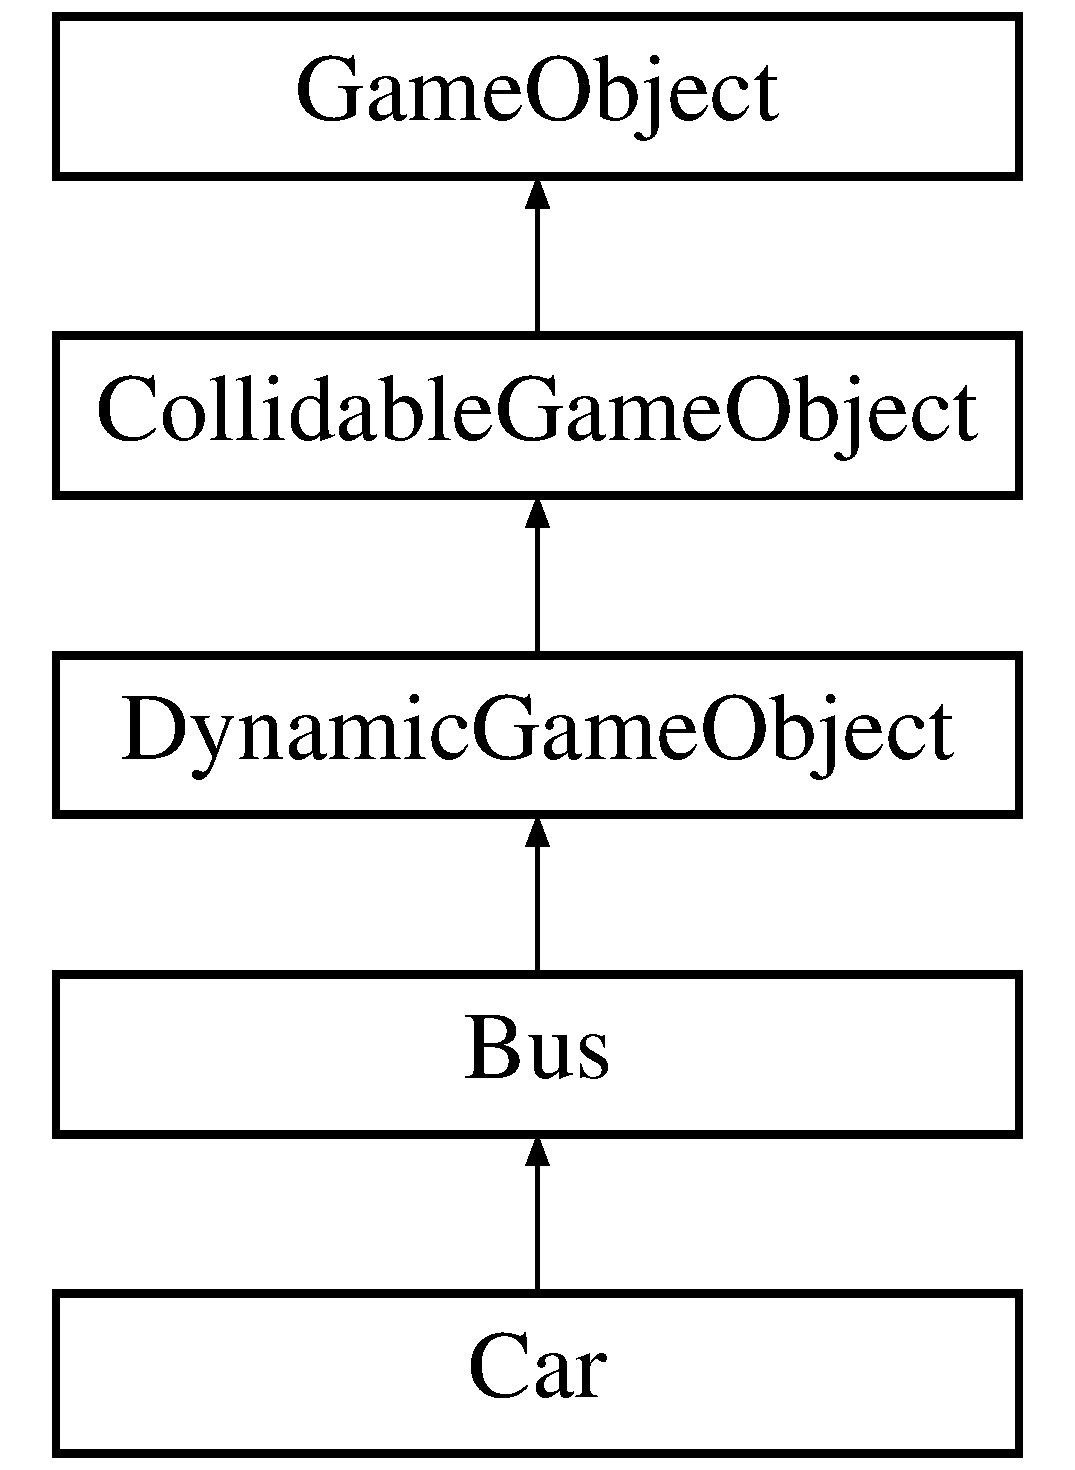
\includegraphics[height=5.000000cm]{class_bus}
\end{center}
\end{figure}
\subsection*{Public Member Functions}
\begin{DoxyCompactItemize}
\item 
\hyperlink{class_bus_a262505182585ed32d38dda38ab68147f}{Bus} (\hyperlink{class_vector3}{Vector3} pos, \hyperlink{class_vector3}{Vector3} \hyperlink{class_dynamic_game_object_a54cb8a3a5fe8314cd5751f223b2b49ae}{speed}, bool going\+Right, \hyperlink{_game_object_8h_a57678b60d65afb213d04a6b090c64a08}{Game\+Object\+Type} type=\hyperlink{_game_object_8h_a57678b60d65afb213d04a6b090c64a08a885a6a40e3fde5dfec3db7fefea61f9b}{B\+US}, \hyperlink{class_vector3}{Vector3} min=\hyperlink{class_vector3}{Vector3}(0, 0, 0), \hyperlink{class_vector3}{Vector3} max=\hyperlink{class_vector3}{Vector3}(3, 1, 1))
\item 
virtual void \hyperlink{class_bus_a4f917c97b2fc287fc9b01795250f591d}{respawn} ()
\item 
void \hyperlink{class_bus_a7bff316b767441b92f8e82f17a44fbf7}{init} () override
\item 
void \hyperlink{class_bus_ad07157ce2a50211ea599d040da7a4517}{update} (int \hyperlink{_game_manager_8h_afea6a95c7a1c119b7106a4c735eb259d}{delta\+Time}) final
\item 
void \hyperlink{class_bus_a0fe709af4b2ca86583d8647f323c231c}{render} () override
\end{DoxyCompactItemize}
\subsection*{Public Attributes}
\begin{DoxyCompactItemize}
\item 
bool \hyperlink{class_bus_ad27976dad538444f6e95212834d989a8}{is\+Going\+Right} = false
\item 
float \hyperlink{class_bus_ab2899ff7aa88eccd9ec84a79355b671b}{angle} = 0
\end{DoxyCompactItemize}
\subsection*{Additional Inherited Members}


\subsection{Constructor \& Destructor Documentation}
\mbox{\Hypertarget{class_bus_a262505182585ed32d38dda38ab68147f}\label{class_bus_a262505182585ed32d38dda38ab68147f}} 
\index{Bus@{Bus}!Bus@{Bus}}
\index{Bus@{Bus}!Bus@{Bus}}
\subsubsection{\texorpdfstring{Bus()}{Bus()}}
{\footnotesize\ttfamily Bus\+::\+Bus (\begin{DoxyParamCaption}\item[{\hyperlink{class_vector3}{Vector3}}]{pos,  }\item[{\hyperlink{class_vector3}{Vector3}}]{speed,  }\item[{bool}]{going\+Right,  }\item[{\hyperlink{_game_object_8h_a57678b60d65afb213d04a6b090c64a08}{Game\+Object\+Type}}]{type = {\ttfamily \hyperlink{_game_object_8h_a57678b60d65afb213d04a6b090c64a08a885a6a40e3fde5dfec3db7fefea61f9b}{B\+US}},  }\item[{\hyperlink{class_vector3}{Vector3}}]{min = {\ttfamily \hyperlink{class_vector3}{Vector3}(0,~0,~0)},  }\item[{\hyperlink{class_vector3}{Vector3}}]{max = {\ttfamily \hyperlink{class_vector3}{Vector3}(3,~1,~1)} }\end{DoxyParamCaption})\hspace{0.3cm}{\ttfamily [inline]}}



\subsection{Member Function Documentation}
\mbox{\Hypertarget{class_bus_a7bff316b767441b92f8e82f17a44fbf7}\label{class_bus_a7bff316b767441b92f8e82f17a44fbf7}} 
\index{Bus@{Bus}!init@{init}}
\index{init@{init}!Bus@{Bus}}
\subsubsection{\texorpdfstring{init()}{init()}}
{\footnotesize\ttfamily void Bus\+::init (\begin{DoxyParamCaption}{ }\end{DoxyParamCaption})\hspace{0.3cm}{\ttfamily [inline]}, {\ttfamily [override]}, {\ttfamily [virtual]}}



Reimplemented from \hyperlink{class_game_object_aecb2c1b9f69715d854f7604d5d7978ec}{Game\+Object}.



Reimplemented in \hyperlink{class_car_ae7d4da15bf41cc2d36465129372f2a71}{Car}.

\mbox{\Hypertarget{class_bus_a0fe709af4b2ca86583d8647f323c231c}\label{class_bus_a0fe709af4b2ca86583d8647f323c231c}} 
\index{Bus@{Bus}!render@{render}}
\index{render@{render}!Bus@{Bus}}
\subsubsection{\texorpdfstring{render()}{render()}}
{\footnotesize\ttfamily void Bus\+::render (\begin{DoxyParamCaption}{ }\end{DoxyParamCaption})\hspace{0.3cm}{\ttfamily [inline]}, {\ttfamily [override]}, {\ttfamily [virtual]}}



Reimplemented from \hyperlink{class_game_object_a484efb66a7a27c101e84c11d9905d7a6}{Game\+Object}.



Reimplemented in \hyperlink{class_car_a52c7156c403d267444de3d4813fffba2}{Car}.

\mbox{\Hypertarget{class_bus_a4f917c97b2fc287fc9b01795250f591d}\label{class_bus_a4f917c97b2fc287fc9b01795250f591d}} 
\index{Bus@{Bus}!respawn@{respawn}}
\index{respawn@{respawn}!Bus@{Bus}}
\subsubsection{\texorpdfstring{respawn()}{respawn()}}
{\footnotesize\ttfamily virtual void Bus\+::respawn (\begin{DoxyParamCaption}{ }\end{DoxyParamCaption})\hspace{0.3cm}{\ttfamily [inline]}, {\ttfamily [virtual]}}

\mbox{\Hypertarget{class_bus_ad07157ce2a50211ea599d040da7a4517}\label{class_bus_ad07157ce2a50211ea599d040da7a4517}} 
\index{Bus@{Bus}!update@{update}}
\index{update@{update}!Bus@{Bus}}
\subsubsection{\texorpdfstring{update()}{update()}}
{\footnotesize\ttfamily void Bus\+::update (\begin{DoxyParamCaption}\item[{int}]{delta\+Time }\end{DoxyParamCaption})\hspace{0.3cm}{\ttfamily [inline]}, {\ttfamily [final]}, {\ttfamily [virtual]}}



Reimplemented from \hyperlink{class_dynamic_game_object_aaa505b57d131bbbce44d500ec2ca0e83}{Dynamic\+Game\+Object}.



\subsection{Member Data Documentation}
\mbox{\Hypertarget{class_bus_ab2899ff7aa88eccd9ec84a79355b671b}\label{class_bus_ab2899ff7aa88eccd9ec84a79355b671b}} 
\index{Bus@{Bus}!angle@{angle}}
\index{angle@{angle}!Bus@{Bus}}
\subsubsection{\texorpdfstring{angle}{angle}}
{\footnotesize\ttfamily float Bus\+::angle = 0}

\mbox{\Hypertarget{class_bus_ad27976dad538444f6e95212834d989a8}\label{class_bus_ad27976dad538444f6e95212834d989a8}} 
\index{Bus@{Bus}!is\+Going\+Right@{is\+Going\+Right}}
\index{is\+Going\+Right@{is\+Going\+Right}!Bus@{Bus}}
\subsubsection{\texorpdfstring{is\+Going\+Right}{isGoingRight}}
{\footnotesize\ttfamily bool Bus\+::is\+Going\+Right = false}



The documentation for this class was generated from the following file\+:\begin{DoxyCompactItemize}
\item 
/\+Users/matya/\+A\+V\+T7/src/objects/\hyperlink{_bus_8h}{Bus.\+h}\end{DoxyCompactItemize}

\hypertarget{class_camera}{}\section{Camera Class Reference}
\label{class_camera}\index{Camera@{Camera}}


{\ttfamily \#include $<$Camera.\+h$>$}

Inheritance diagram for Camera\+:\begin{figure}[H]
\begin{center}
\leavevmode
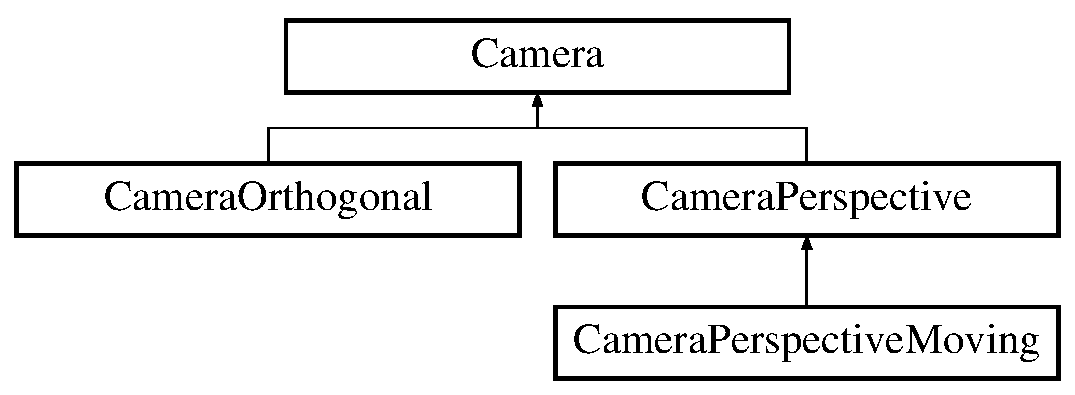
\includegraphics[height=3.000000cm]{class_camera}
\end{center}
\end{figure}
\subsection*{Public Member Functions}
\begin{DoxyCompactItemize}
\item 
\hyperlink{class_camera_a92eff4b0c0b15b38222318840552d27b}{Camera} (\hyperlink{class_vector3}{Vector3} \hyperlink{class_camera_a2c4c5bcf8f5885968d4e5ebc28074846}{pos})
\item 
virtual void \hyperlink{class_camera_a151cbf3898d114f0a8bf079a3e90e7f4}{view} ()=0
\item 
virtual void \hyperlink{class_camera_a5b50ba31455a712ec09561105c12c7c2}{project} (int w, int h)=0
\end{DoxyCompactItemize}
\subsection*{Public Attributes}
\begin{DoxyCompactItemize}
\item 
float \hyperlink{class_camera_a838139083987e3ede449183558e2bd61}{nearp} = 0.\+1f
\item 
float \hyperlink{class_camera_ae19883a49359025f85d96d20c774fe4b}{farp} = 1000.\+0f
\item 
\hyperlink{class_vector3}{Vector3} \hyperlink{class_camera_a2c4c5bcf8f5885968d4e5ebc28074846}{pos}
\end{DoxyCompactItemize}


\subsection{Constructor \& Destructor Documentation}
\mbox{\Hypertarget{class_camera_a92eff4b0c0b15b38222318840552d27b}\label{class_camera_a92eff4b0c0b15b38222318840552d27b}} 
\index{Camera@{Camera}!Camera@{Camera}}
\index{Camera@{Camera}!Camera@{Camera}}
\subsubsection{\texorpdfstring{Camera()}{Camera()}}
{\footnotesize\ttfamily Camera\+::\+Camera (\begin{DoxyParamCaption}\item[{\hyperlink{class_vector3}{Vector3}}]{pos }\end{DoxyParamCaption})\hspace{0.3cm}{\ttfamily [inline]}, {\ttfamily [explicit]}}



\subsection{Member Function Documentation}
\mbox{\Hypertarget{class_camera_a5b50ba31455a712ec09561105c12c7c2}\label{class_camera_a5b50ba31455a712ec09561105c12c7c2}} 
\index{Camera@{Camera}!project@{project}}
\index{project@{project}!Camera@{Camera}}
\subsubsection{\texorpdfstring{project()}{project()}}
{\footnotesize\ttfamily virtual void Camera\+::project (\begin{DoxyParamCaption}\item[{int}]{w,  }\item[{int}]{h }\end{DoxyParamCaption})\hspace{0.3cm}{\ttfamily [pure virtual]}}



Implemented in \hyperlink{class_camera_perspective_a841f648f4131897ec632cfcb55facf97}{Camera\+Perspective}, and \hyperlink{class_camera_orthogonal_a593df7d7b84de30d312e31ffed831d9c}{Camera\+Orthogonal}.

\mbox{\Hypertarget{class_camera_a151cbf3898d114f0a8bf079a3e90e7f4}\label{class_camera_a151cbf3898d114f0a8bf079a3e90e7f4}} 
\index{Camera@{Camera}!view@{view}}
\index{view@{view}!Camera@{Camera}}
\subsubsection{\texorpdfstring{view()}{view()}}
{\footnotesize\ttfamily virtual void Camera\+::view (\begin{DoxyParamCaption}{ }\end{DoxyParamCaption})\hspace{0.3cm}{\ttfamily [pure virtual]}}



Implemented in \hyperlink{class_camera_perspective_a6605f8288ea01b0d647213df88d2a45b}{Camera\+Perspective}, and \hyperlink{class_camera_orthogonal_aba42e2f1ce347576e6ab83e45a8d7ed9}{Camera\+Orthogonal}.



\subsection{Member Data Documentation}
\mbox{\Hypertarget{class_camera_ae19883a49359025f85d96d20c774fe4b}\label{class_camera_ae19883a49359025f85d96d20c774fe4b}} 
\index{Camera@{Camera}!farp@{farp}}
\index{farp@{farp}!Camera@{Camera}}
\subsubsection{\texorpdfstring{farp}{farp}}
{\footnotesize\ttfamily float Camera\+::farp = 1000.\+0f}

\mbox{\Hypertarget{class_camera_a838139083987e3ede449183558e2bd61}\label{class_camera_a838139083987e3ede449183558e2bd61}} 
\index{Camera@{Camera}!nearp@{nearp}}
\index{nearp@{nearp}!Camera@{Camera}}
\subsubsection{\texorpdfstring{nearp}{nearp}}
{\footnotesize\ttfamily float Camera\+::nearp = 0.\+1f}

\mbox{\Hypertarget{class_camera_a2c4c5bcf8f5885968d4e5ebc28074846}\label{class_camera_a2c4c5bcf8f5885968d4e5ebc28074846}} 
\index{Camera@{Camera}!pos@{pos}}
\index{pos@{pos}!Camera@{Camera}}
\subsubsection{\texorpdfstring{pos}{pos}}
{\footnotesize\ttfamily \hyperlink{class_vector3}{Vector3} Camera\+::pos}



The documentation for this class was generated from the following file\+:\begin{DoxyCompactItemize}
\item 
/\+Users/matya/\+A\+V\+T7/src/\hyperlink{_camera_8h}{Camera.\+h}\end{DoxyCompactItemize}

\hypertarget{class_camera_orthogonal}{}\section{Camera\+Orthogonal Class Reference}
\label{class_camera_orthogonal}\index{Camera\+Orthogonal@{Camera\+Orthogonal}}


{\ttfamily \#include $<$Camera\+Orthogonal.\+h$>$}

Inheritance diagram for Camera\+Orthogonal\+:\begin{figure}[H]
\begin{center}
\leavevmode
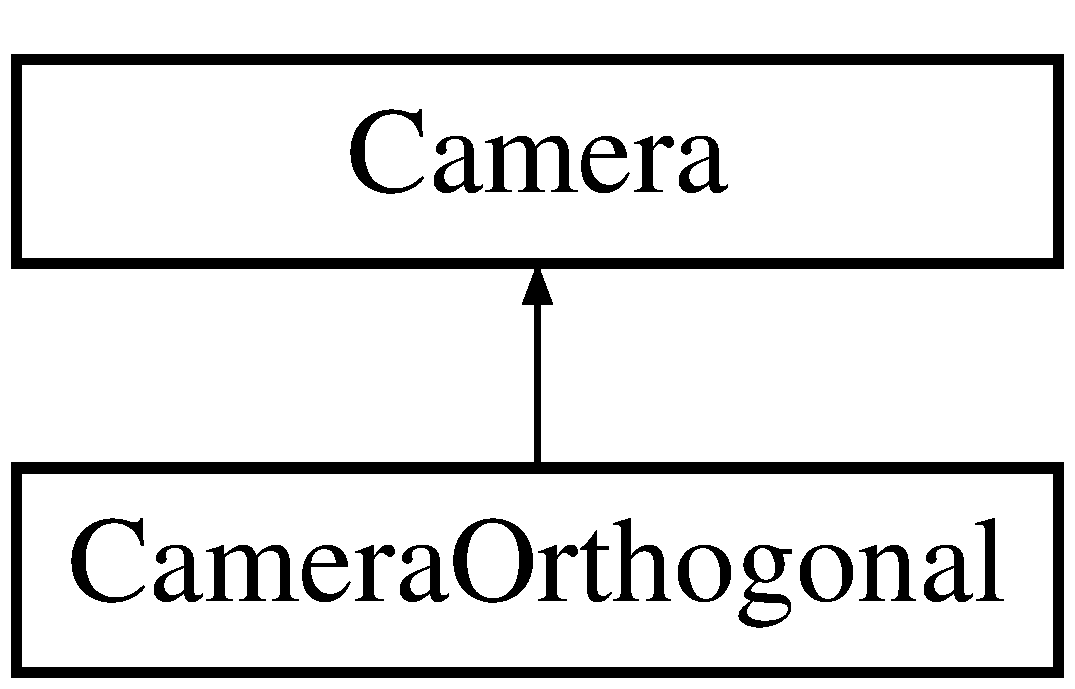
\includegraphics[height=2.000000cm]{class_camera_orthogonal}
\end{center}
\end{figure}
\subsection*{Public Member Functions}
\begin{DoxyCompactItemize}
\item 
\hyperlink{class_camera_orthogonal_aabed9106e5ae8c9661afba065f8cd6ad}{Camera\+Orthogonal} (float \hyperlink{class_camera_orthogonal_a8a6d6d01dae35b1ddb7de2e06f7a2133}{left}, float \hyperlink{class_camera_orthogonal_a7f25057c59bc911d92b99d7f649fe790}{right}, float \hyperlink{class_camera_orthogonal_a87037becad1484ffdc5cd9a051716d6e}{bottom}, float \hyperlink{class_camera_orthogonal_afb3bdd5249f1e5d690624812bac24dd7}{top})
\item 
void \hyperlink{class_camera_orthogonal_aba42e2f1ce347576e6ab83e45a8d7ed9}{view} () final
\item 
void \hyperlink{class_camera_orthogonal_a593df7d7b84de30d312e31ffed831d9c}{project} (int w, int h) final
\end{DoxyCompactItemize}
\subsection*{Public Attributes}
\begin{DoxyCompactItemize}
\item 
float \hyperlink{class_camera_orthogonal_a8a6d6d01dae35b1ddb7de2e06f7a2133}{left}
\item 
float \hyperlink{class_camera_orthogonal_a7f25057c59bc911d92b99d7f649fe790}{right}
\item 
float \hyperlink{class_camera_orthogonal_afb3bdd5249f1e5d690624812bac24dd7}{top}
\item 
float \hyperlink{class_camera_orthogonal_a87037becad1484ffdc5cd9a051716d6e}{bottom}
\end{DoxyCompactItemize}


\subsection{Constructor \& Destructor Documentation}
\mbox{\Hypertarget{class_camera_orthogonal_aabed9106e5ae8c9661afba065f8cd6ad}\label{class_camera_orthogonal_aabed9106e5ae8c9661afba065f8cd6ad}} 
\index{Camera\+Orthogonal@{Camera\+Orthogonal}!Camera\+Orthogonal@{Camera\+Orthogonal}}
\index{Camera\+Orthogonal@{Camera\+Orthogonal}!Camera\+Orthogonal@{Camera\+Orthogonal}}
\subsubsection{\texorpdfstring{Camera\+Orthogonal()}{CameraOrthogonal()}}
{\footnotesize\ttfamily Camera\+Orthogonal\+::\+Camera\+Orthogonal (\begin{DoxyParamCaption}\item[{float}]{left,  }\item[{float}]{right,  }\item[{float}]{bottom,  }\item[{float}]{top }\end{DoxyParamCaption})\hspace{0.3cm}{\ttfamily [inline]}}



\subsection{Member Function Documentation}
\mbox{\Hypertarget{class_camera_orthogonal_a593df7d7b84de30d312e31ffed831d9c}\label{class_camera_orthogonal_a593df7d7b84de30d312e31ffed831d9c}} 
\index{Camera\+Orthogonal@{Camera\+Orthogonal}!project@{project}}
\index{project@{project}!Camera\+Orthogonal@{Camera\+Orthogonal}}
\subsubsection{\texorpdfstring{project()}{project()}}
{\footnotesize\ttfamily void Camera\+Orthogonal\+::project (\begin{DoxyParamCaption}\item[{int}]{w,  }\item[{int}]{h }\end{DoxyParamCaption})\hspace{0.3cm}{\ttfamily [inline]}, {\ttfamily [final]}, {\ttfamily [virtual]}}



Implements \hyperlink{class_camera_a5b50ba31455a712ec09561105c12c7c2}{Camera}.

\mbox{\Hypertarget{class_camera_orthogonal_aba42e2f1ce347576e6ab83e45a8d7ed9}\label{class_camera_orthogonal_aba42e2f1ce347576e6ab83e45a8d7ed9}} 
\index{Camera\+Orthogonal@{Camera\+Orthogonal}!view@{view}}
\index{view@{view}!Camera\+Orthogonal@{Camera\+Orthogonal}}
\subsubsection{\texorpdfstring{view()}{view()}}
{\footnotesize\ttfamily void Camera\+Orthogonal\+::view (\begin{DoxyParamCaption}{ }\end{DoxyParamCaption})\hspace{0.3cm}{\ttfamily [inline]}, {\ttfamily [final]}, {\ttfamily [virtual]}}



Implements \hyperlink{class_camera_a151cbf3898d114f0a8bf079a3e90e7f4}{Camera}.



\subsection{Member Data Documentation}
\mbox{\Hypertarget{class_camera_orthogonal_a87037becad1484ffdc5cd9a051716d6e}\label{class_camera_orthogonal_a87037becad1484ffdc5cd9a051716d6e}} 
\index{Camera\+Orthogonal@{Camera\+Orthogonal}!bottom@{bottom}}
\index{bottom@{bottom}!Camera\+Orthogonal@{Camera\+Orthogonal}}
\subsubsection{\texorpdfstring{bottom}{bottom}}
{\footnotesize\ttfamily float Camera\+Orthogonal\+::bottom}

\mbox{\Hypertarget{class_camera_orthogonal_a8a6d6d01dae35b1ddb7de2e06f7a2133}\label{class_camera_orthogonal_a8a6d6d01dae35b1ddb7de2e06f7a2133}} 
\index{Camera\+Orthogonal@{Camera\+Orthogonal}!left@{left}}
\index{left@{left}!Camera\+Orthogonal@{Camera\+Orthogonal}}
\subsubsection{\texorpdfstring{left}{left}}
{\footnotesize\ttfamily float Camera\+Orthogonal\+::left}

\mbox{\Hypertarget{class_camera_orthogonal_a7f25057c59bc911d92b99d7f649fe790}\label{class_camera_orthogonal_a7f25057c59bc911d92b99d7f649fe790}} 
\index{Camera\+Orthogonal@{Camera\+Orthogonal}!right@{right}}
\index{right@{right}!Camera\+Orthogonal@{Camera\+Orthogonal}}
\subsubsection{\texorpdfstring{right}{right}}
{\footnotesize\ttfamily float Camera\+Orthogonal\+::right}

\mbox{\Hypertarget{class_camera_orthogonal_afb3bdd5249f1e5d690624812bac24dd7}\label{class_camera_orthogonal_afb3bdd5249f1e5d690624812bac24dd7}} 
\index{Camera\+Orthogonal@{Camera\+Orthogonal}!top@{top}}
\index{top@{top}!Camera\+Orthogonal@{Camera\+Orthogonal}}
\subsubsection{\texorpdfstring{top}{top}}
{\footnotesize\ttfamily float Camera\+Orthogonal\+::top}



The documentation for this class was generated from the following file\+:\begin{DoxyCompactItemize}
\item 
/\+Users/matya/\+A\+V\+T7/src/\hyperlink{_camera_orthogonal_8h}{Camera\+Orthogonal.\+h}\end{DoxyCompactItemize}

\hypertarget{class_camera_perspective}{}\section{Camera\+Perspective Class Reference}
\label{class_camera_perspective}\index{Camera\+Perspective@{Camera\+Perspective}}


{\ttfamily \#include $<$Camera\+Perspective.\+h$>$}

Inheritance diagram for Camera\+Perspective\+:\begin{figure}[H]
\begin{center}
\leavevmode
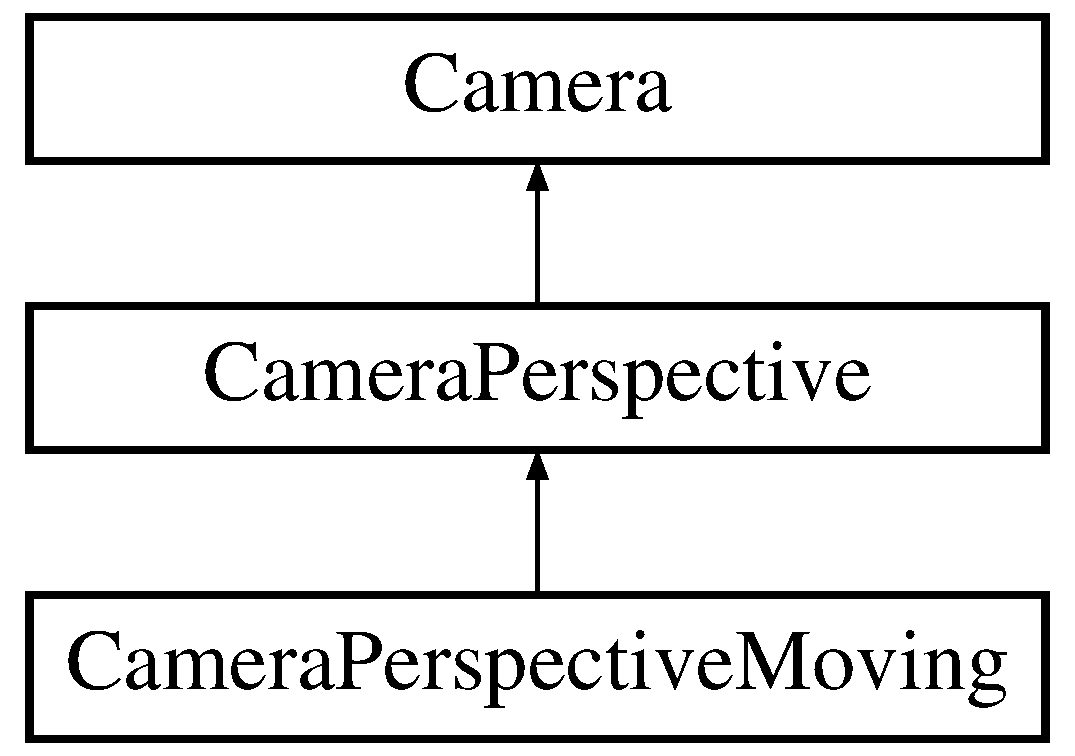
\includegraphics[height=3.000000cm]{class_camera_perspective}
\end{center}
\end{figure}
\subsection*{Public Member Functions}
\begin{DoxyCompactItemize}
\item 
\hyperlink{class_camera_perspective_a44735f45c240e39cd10dcae59dc752d3}{Camera\+Perspective} (float \hyperlink{class_camera_perspective_adb49aa14a62f537f810038351b141a36}{r}, float \hyperlink{class_camera_perspective_a93009a48069d0d671317c5d9f7d66963}{alpha}, float \hyperlink{class_camera_perspective_a3545402762e444abd3cb90ea9d2e72ca}{beta}, \hyperlink{class_vector3}{Vector3} \hyperlink{class_camera_a2c4c5bcf8f5885968d4e5ebc28074846}{pos})
\item 
void \hyperlink{class_camera_perspective_aaaa30cbae530a2d4716a3f333df2d240}{mouse\+Update} (float \hyperlink{class_camera_perspective_adb49aa14a62f537f810038351b141a36}{r}, float \hyperlink{class_camera_perspective_a93009a48069d0d671317c5d9f7d66963}{alpha}, float \hyperlink{class_camera_perspective_a3545402762e444abd3cb90ea9d2e72ca}{beta})
\item 
void \hyperlink{class_camera_perspective_a6605f8288ea01b0d647213df88d2a45b}{view} () override
\item 
void \hyperlink{class_camera_perspective_a841f648f4131897ec632cfcb55facf97}{project} (int w, int h) override
\item 
void \hyperlink{class_camera_perspective_a3e3875dbaf831674e33e5aee8d179224}{print\+Coordinates} ()
\end{DoxyCompactItemize}
\subsection*{Public Attributes}
\begin{DoxyCompactItemize}
\item 
float \hyperlink{class_camera_perspective_a53ed75a72568390a0a42c217baf07221}{fov} = 53.\+13f
\item 
float \hyperlink{class_camera_perspective_adb49aa14a62f537f810038351b141a36}{r} = 20.\+0f
\item 
float \hyperlink{class_camera_perspective_a93009a48069d0d671317c5d9f7d66963}{alpha} = 0.\+0f
\item 
float \hyperlink{class_camera_perspective_a3545402762e444abd3cb90ea9d2e72ca}{beta} = 40.\+0f
\item 
\hyperlink{class_vector3}{Vector3} \hyperlink{class_camera_perspective_afe2ca37c029acb558350b2fe1025e9c5}{local\+Pos} = \hyperlink{class_vector3}{Vector3}()
\end{DoxyCompactItemize}


\subsection{Constructor \& Destructor Documentation}
\mbox{\Hypertarget{class_camera_perspective_a44735f45c240e39cd10dcae59dc752d3}\label{class_camera_perspective_a44735f45c240e39cd10dcae59dc752d3}} 
\index{Camera\+Perspective@{Camera\+Perspective}!Camera\+Perspective@{Camera\+Perspective}}
\index{Camera\+Perspective@{Camera\+Perspective}!Camera\+Perspective@{Camera\+Perspective}}
\subsubsection{\texorpdfstring{Camera\+Perspective()}{CameraPerspective()}}
{\footnotesize\ttfamily Camera\+Perspective\+::\+Camera\+Perspective (\begin{DoxyParamCaption}\item[{float}]{r,  }\item[{float}]{alpha,  }\item[{float}]{beta,  }\item[{\hyperlink{class_vector3}{Vector3}}]{pos }\end{DoxyParamCaption})\hspace{0.3cm}{\ttfamily [inline]}}



\subsection{Member Function Documentation}
\mbox{\Hypertarget{class_camera_perspective_aaaa30cbae530a2d4716a3f333df2d240}\label{class_camera_perspective_aaaa30cbae530a2d4716a3f333df2d240}} 
\index{Camera\+Perspective@{Camera\+Perspective}!mouse\+Update@{mouse\+Update}}
\index{mouse\+Update@{mouse\+Update}!Camera\+Perspective@{Camera\+Perspective}}
\subsubsection{\texorpdfstring{mouse\+Update()}{mouseUpdate()}}
{\footnotesize\ttfamily void Camera\+Perspective\+::mouse\+Update (\begin{DoxyParamCaption}\item[{float}]{r,  }\item[{float}]{alpha,  }\item[{float}]{beta }\end{DoxyParamCaption})\hspace{0.3cm}{\ttfamily [inline]}}

\mbox{\Hypertarget{class_camera_perspective_a3e3875dbaf831674e33e5aee8d179224}\label{class_camera_perspective_a3e3875dbaf831674e33e5aee8d179224}} 
\index{Camera\+Perspective@{Camera\+Perspective}!print\+Coordinates@{print\+Coordinates}}
\index{print\+Coordinates@{print\+Coordinates}!Camera\+Perspective@{Camera\+Perspective}}
\subsubsection{\texorpdfstring{print\+Coordinates()}{printCoordinates()}}
{\footnotesize\ttfamily void Camera\+Perspective\+::print\+Coordinates (\begin{DoxyParamCaption}{ }\end{DoxyParamCaption})\hspace{0.3cm}{\ttfamily [inline]}}

\mbox{\Hypertarget{class_camera_perspective_a841f648f4131897ec632cfcb55facf97}\label{class_camera_perspective_a841f648f4131897ec632cfcb55facf97}} 
\index{Camera\+Perspective@{Camera\+Perspective}!project@{project}}
\index{project@{project}!Camera\+Perspective@{Camera\+Perspective}}
\subsubsection{\texorpdfstring{project()}{project()}}
{\footnotesize\ttfamily void Camera\+Perspective\+::project (\begin{DoxyParamCaption}\item[{int}]{w,  }\item[{int}]{h }\end{DoxyParamCaption})\hspace{0.3cm}{\ttfamily [inline]}, {\ttfamily [override]}, {\ttfamily [virtual]}}



Implements \hyperlink{class_camera_a5b50ba31455a712ec09561105c12c7c2}{Camera}.

\mbox{\Hypertarget{class_camera_perspective_a6605f8288ea01b0d647213df88d2a45b}\label{class_camera_perspective_a6605f8288ea01b0d647213df88d2a45b}} 
\index{Camera\+Perspective@{Camera\+Perspective}!view@{view}}
\index{view@{view}!Camera\+Perspective@{Camera\+Perspective}}
\subsubsection{\texorpdfstring{view()}{view()}}
{\footnotesize\ttfamily void Camera\+Perspective\+::view (\begin{DoxyParamCaption}{ }\end{DoxyParamCaption})\hspace{0.3cm}{\ttfamily [inline]}, {\ttfamily [override]}, {\ttfamily [virtual]}}



Implements \hyperlink{class_camera_a151cbf3898d114f0a8bf079a3e90e7f4}{Camera}.



\subsection{Member Data Documentation}
\mbox{\Hypertarget{class_camera_perspective_a93009a48069d0d671317c5d9f7d66963}\label{class_camera_perspective_a93009a48069d0d671317c5d9f7d66963}} 
\index{Camera\+Perspective@{Camera\+Perspective}!alpha@{alpha}}
\index{alpha@{alpha}!Camera\+Perspective@{Camera\+Perspective}}
\subsubsection{\texorpdfstring{alpha}{alpha}}
{\footnotesize\ttfamily float Camera\+Perspective\+::alpha = 0.\+0f}

\mbox{\Hypertarget{class_camera_perspective_a3545402762e444abd3cb90ea9d2e72ca}\label{class_camera_perspective_a3545402762e444abd3cb90ea9d2e72ca}} 
\index{Camera\+Perspective@{Camera\+Perspective}!beta@{beta}}
\index{beta@{beta}!Camera\+Perspective@{Camera\+Perspective}}
\subsubsection{\texorpdfstring{beta}{beta}}
{\footnotesize\ttfamily float Camera\+Perspective\+::beta = 40.\+0f}

\mbox{\Hypertarget{class_camera_perspective_a53ed75a72568390a0a42c217baf07221}\label{class_camera_perspective_a53ed75a72568390a0a42c217baf07221}} 
\index{Camera\+Perspective@{Camera\+Perspective}!fov@{fov}}
\index{fov@{fov}!Camera\+Perspective@{Camera\+Perspective}}
\subsubsection{\texorpdfstring{fov}{fov}}
{\footnotesize\ttfamily float Camera\+Perspective\+::fov = 53.\+13f}

\mbox{\Hypertarget{class_camera_perspective_afe2ca37c029acb558350b2fe1025e9c5}\label{class_camera_perspective_afe2ca37c029acb558350b2fe1025e9c5}} 
\index{Camera\+Perspective@{Camera\+Perspective}!local\+Pos@{local\+Pos}}
\index{local\+Pos@{local\+Pos}!Camera\+Perspective@{Camera\+Perspective}}
\subsubsection{\texorpdfstring{local\+Pos}{localPos}}
{\footnotesize\ttfamily \hyperlink{class_vector3}{Vector3} Camera\+Perspective\+::local\+Pos = \hyperlink{class_vector3}{Vector3}()}

\mbox{\Hypertarget{class_camera_perspective_adb49aa14a62f537f810038351b141a36}\label{class_camera_perspective_adb49aa14a62f537f810038351b141a36}} 
\index{Camera\+Perspective@{Camera\+Perspective}!r@{r}}
\index{r@{r}!Camera\+Perspective@{Camera\+Perspective}}
\subsubsection{\texorpdfstring{r}{r}}
{\footnotesize\ttfamily float Camera\+Perspective\+::r = 20.\+0f}



The documentation for this class was generated from the following file\+:\begin{DoxyCompactItemize}
\item 
/\+Users/matya/\+A\+V\+T7/src/\hyperlink{_camera_perspective_8h}{Camera\+Perspective.\+h}\end{DoxyCompactItemize}

\hypertarget{class_camera_perspective_moving}{}\section{Camera\+Perspective\+Moving Class Reference}
\label{class_camera_perspective_moving}\index{Camera\+Perspective\+Moving@{Camera\+Perspective\+Moving}}


{\ttfamily \#include $<$Camera\+Perspective\+Moving.\+h$>$}

Inheritance diagram for Camera\+Perspective\+Moving\+:\begin{figure}[H]
\begin{center}
\leavevmode
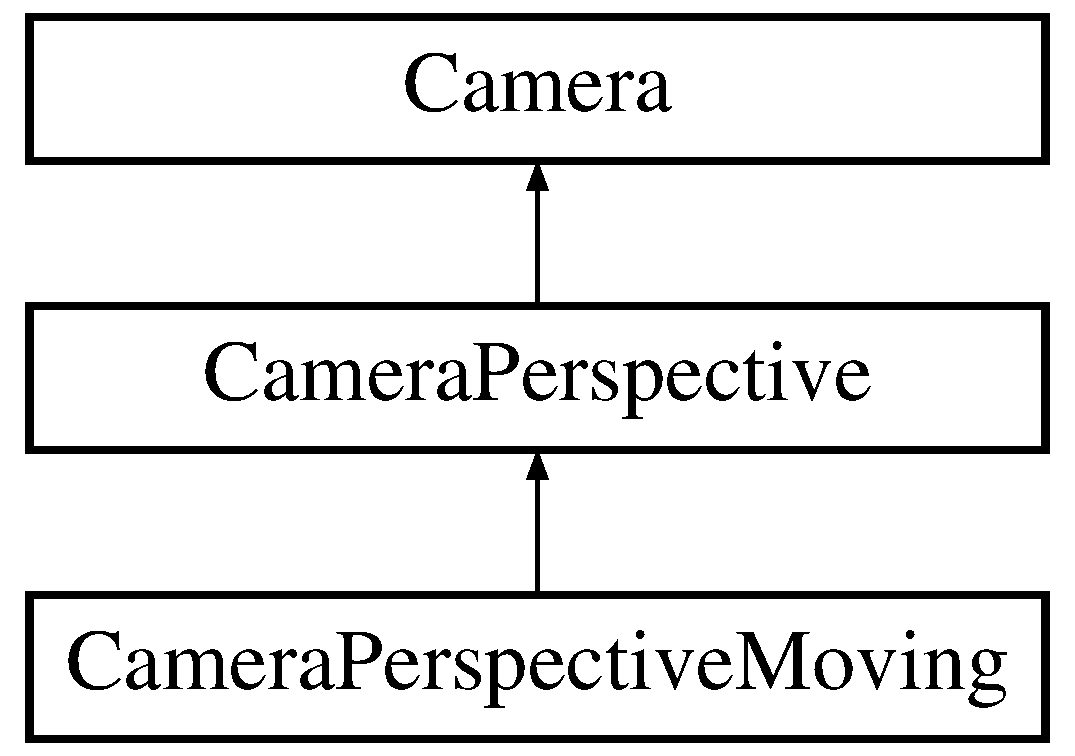
\includegraphics[height=3.000000cm]{class_camera_perspective_moving}
\end{center}
\end{figure}
\subsection*{Public Member Functions}
\begin{DoxyCompactItemize}
\item 
\hyperlink{class_camera_perspective_moving_a61a3b32e7c149c9aa7091303f831d6c1}{Camera\+Perspective\+Moving} (float \hyperlink{class_camera_perspective_adb49aa14a62f537f810038351b141a36}{r}, float \hyperlink{class_camera_perspective_a93009a48069d0d671317c5d9f7d66963}{alpha}, float \hyperlink{class_camera_perspective_a3545402762e444abd3cb90ea9d2e72ca}{beta}, \hyperlink{class_vector3}{Vector3} \hyperlink{class_camera_a2c4c5bcf8f5885968d4e5ebc28074846}{pos})
\item 
void \hyperlink{class_camera_perspective_moving_ace1cd58845d0122e284a5ebecb2528ce}{process\+Mouse\+Buttons} (int button, int state, int xx, int yy)
\item 
void \hyperlink{class_camera_perspective_moving_aacc461e1ac1912f0aefdeafcf04ccdbf}{process\+Mouse\+Motion} (int xx, int yy)
\item 
void \hyperlink{class_camera_perspective_moving_a7feb0b10588b45d72c894b1366da5811}{mouse\+Wheel} (int wheel, int direction, int x, int y)
\end{DoxyCompactItemize}
\subsection*{Public Attributes}
\begin{DoxyCompactItemize}
\item 
int \hyperlink{class_camera_perspective_moving_a69b3b2a9640c959b047efe17baea370c}{startX} = 0
\item 
int \hyperlink{class_camera_perspective_moving_a8a18360e9a24f78c32fd5e7d667a24e4}{startY} = 0
\item 
int \hyperlink{class_camera_perspective_moving_acf09c3044b76990c814adc466471a571}{tracking} = 0
\end{DoxyCompactItemize}


\subsection{Constructor \& Destructor Documentation}
\mbox{\Hypertarget{class_camera_perspective_moving_a61a3b32e7c149c9aa7091303f831d6c1}\label{class_camera_perspective_moving_a61a3b32e7c149c9aa7091303f831d6c1}} 
\index{Camera\+Perspective\+Moving@{Camera\+Perspective\+Moving}!Camera\+Perspective\+Moving@{Camera\+Perspective\+Moving}}
\index{Camera\+Perspective\+Moving@{Camera\+Perspective\+Moving}!Camera\+Perspective\+Moving@{Camera\+Perspective\+Moving}}
\subsubsection{\texorpdfstring{Camera\+Perspective\+Moving()}{CameraPerspectiveMoving()}}
{\footnotesize\ttfamily Camera\+Perspective\+Moving\+::\+Camera\+Perspective\+Moving (\begin{DoxyParamCaption}\item[{float}]{r,  }\item[{float}]{alpha,  }\item[{float}]{beta,  }\item[{\hyperlink{class_vector3}{Vector3}}]{pos }\end{DoxyParamCaption})\hspace{0.3cm}{\ttfamily [inline]}}



\subsection{Member Function Documentation}
\mbox{\Hypertarget{class_camera_perspective_moving_a7feb0b10588b45d72c894b1366da5811}\label{class_camera_perspective_moving_a7feb0b10588b45d72c894b1366da5811}} 
\index{Camera\+Perspective\+Moving@{Camera\+Perspective\+Moving}!mouse\+Wheel@{mouse\+Wheel}}
\index{mouse\+Wheel@{mouse\+Wheel}!Camera\+Perspective\+Moving@{Camera\+Perspective\+Moving}}
\subsubsection{\texorpdfstring{mouse\+Wheel()}{mouseWheel()}}
{\footnotesize\ttfamily void Camera\+Perspective\+Moving\+::mouse\+Wheel (\begin{DoxyParamCaption}\item[{int}]{wheel,  }\item[{int}]{direction,  }\item[{int}]{x,  }\item[{int}]{y }\end{DoxyParamCaption})\hspace{0.3cm}{\ttfamily [inline]}}

\mbox{\Hypertarget{class_camera_perspective_moving_ace1cd58845d0122e284a5ebecb2528ce}\label{class_camera_perspective_moving_ace1cd58845d0122e284a5ebecb2528ce}} 
\index{Camera\+Perspective\+Moving@{Camera\+Perspective\+Moving}!process\+Mouse\+Buttons@{process\+Mouse\+Buttons}}
\index{process\+Mouse\+Buttons@{process\+Mouse\+Buttons}!Camera\+Perspective\+Moving@{Camera\+Perspective\+Moving}}
\subsubsection{\texorpdfstring{process\+Mouse\+Buttons()}{processMouseButtons()}}
{\footnotesize\ttfamily void Camera\+Perspective\+Moving\+::process\+Mouse\+Buttons (\begin{DoxyParamCaption}\item[{int}]{button,  }\item[{int}]{state,  }\item[{int}]{xx,  }\item[{int}]{yy }\end{DoxyParamCaption})\hspace{0.3cm}{\ttfamily [inline]}}

\mbox{\Hypertarget{class_camera_perspective_moving_aacc461e1ac1912f0aefdeafcf04ccdbf}\label{class_camera_perspective_moving_aacc461e1ac1912f0aefdeafcf04ccdbf}} 
\index{Camera\+Perspective\+Moving@{Camera\+Perspective\+Moving}!process\+Mouse\+Motion@{process\+Mouse\+Motion}}
\index{process\+Mouse\+Motion@{process\+Mouse\+Motion}!Camera\+Perspective\+Moving@{Camera\+Perspective\+Moving}}
\subsubsection{\texorpdfstring{process\+Mouse\+Motion()}{processMouseMotion()}}
{\footnotesize\ttfamily void Camera\+Perspective\+Moving\+::process\+Mouse\+Motion (\begin{DoxyParamCaption}\item[{int}]{xx,  }\item[{int}]{yy }\end{DoxyParamCaption})\hspace{0.3cm}{\ttfamily [inline]}}



\subsection{Member Data Documentation}
\mbox{\Hypertarget{class_camera_perspective_moving_a69b3b2a9640c959b047efe17baea370c}\label{class_camera_perspective_moving_a69b3b2a9640c959b047efe17baea370c}} 
\index{Camera\+Perspective\+Moving@{Camera\+Perspective\+Moving}!startX@{startX}}
\index{startX@{startX}!Camera\+Perspective\+Moving@{Camera\+Perspective\+Moving}}
\subsubsection{\texorpdfstring{startX}{startX}}
{\footnotesize\ttfamily int Camera\+Perspective\+Moving\+::startX = 0}

\mbox{\Hypertarget{class_camera_perspective_moving_a8a18360e9a24f78c32fd5e7d667a24e4}\label{class_camera_perspective_moving_a8a18360e9a24f78c32fd5e7d667a24e4}} 
\index{Camera\+Perspective\+Moving@{Camera\+Perspective\+Moving}!startY@{startY}}
\index{startY@{startY}!Camera\+Perspective\+Moving@{Camera\+Perspective\+Moving}}
\subsubsection{\texorpdfstring{startY}{startY}}
{\footnotesize\ttfamily int Camera\+Perspective\+Moving\+::startY = 0}

\mbox{\Hypertarget{class_camera_perspective_moving_acf09c3044b76990c814adc466471a571}\label{class_camera_perspective_moving_acf09c3044b76990c814adc466471a571}} 
\index{Camera\+Perspective\+Moving@{Camera\+Perspective\+Moving}!tracking@{tracking}}
\index{tracking@{tracking}!Camera\+Perspective\+Moving@{Camera\+Perspective\+Moving}}
\subsubsection{\texorpdfstring{tracking}{tracking}}
{\footnotesize\ttfamily int Camera\+Perspective\+Moving\+::tracking = 0}



The documentation for this class was generated from the following file\+:\begin{DoxyCompactItemize}
\item 
/\+Users/matya/\+A\+V\+T7/src/\hyperlink{_camera_perspective_moving_8h}{Camera\+Perspective\+Moving.\+h}\end{DoxyCompactItemize}

\hypertarget{class_car}{}\section{Car Class Reference}
\label{class_car}\index{Car@{Car}}


{\ttfamily \#include $<$Car.\+h$>$}

Inheritance diagram for Car\+:\begin{figure}[H]
\begin{center}
\leavevmode
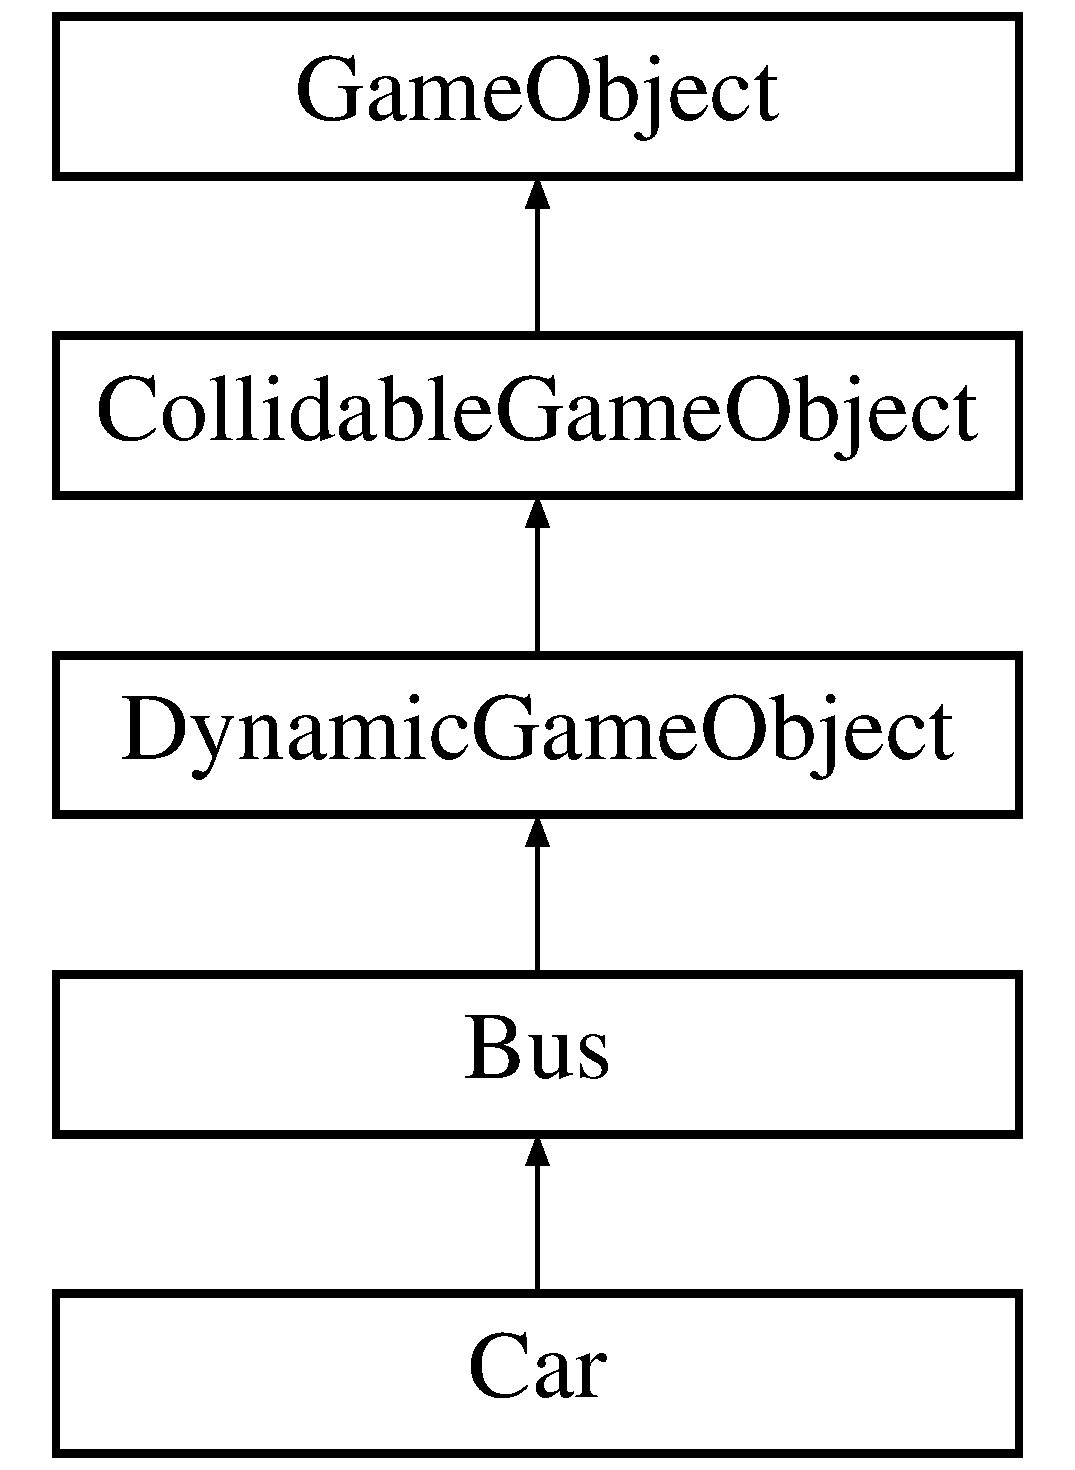
\includegraphics[height=5.000000cm]{class_car}
\end{center}
\end{figure}
\subsection*{Public Member Functions}
\begin{DoxyCompactItemize}
\item 
\hyperlink{class_car_a8eefa9ceb6ad217618cbd96c3be55aca}{Car} (\hyperlink{class_vector3}{Vector3} pos, \hyperlink{class_vector3}{Vector3} \hyperlink{class_dynamic_game_object_a54cb8a3a5fe8314cd5751f223b2b49ae}{speed}, bool going\+Right)
\item 
void \hyperlink{class_car_ae7d4da15bf41cc2d36465129372f2a71}{init} () override
\item 
void \hyperlink{class_car_a52c7156c403d267444de3d4813fffba2}{render} () override
\end{DoxyCompactItemize}
\subsection*{Additional Inherited Members}


\subsection{Constructor \& Destructor Documentation}
\mbox{\Hypertarget{class_car_a8eefa9ceb6ad217618cbd96c3be55aca}\label{class_car_a8eefa9ceb6ad217618cbd96c3be55aca}} 
\index{Car@{Car}!Car@{Car}}
\index{Car@{Car}!Car@{Car}}
\subsubsection{\texorpdfstring{Car()}{Car()}}
{\footnotesize\ttfamily Car\+::\+Car (\begin{DoxyParamCaption}\item[{\hyperlink{class_vector3}{Vector3}}]{pos,  }\item[{\hyperlink{class_vector3}{Vector3}}]{speed,  }\item[{bool}]{going\+Right }\end{DoxyParamCaption})\hspace{0.3cm}{\ttfamily [inline]}}



\subsection{Member Function Documentation}
\mbox{\Hypertarget{class_car_ae7d4da15bf41cc2d36465129372f2a71}\label{class_car_ae7d4da15bf41cc2d36465129372f2a71}} 
\index{Car@{Car}!init@{init}}
\index{init@{init}!Car@{Car}}
\subsubsection{\texorpdfstring{init()}{init()}}
{\footnotesize\ttfamily void Car\+::init (\begin{DoxyParamCaption}{ }\end{DoxyParamCaption})\hspace{0.3cm}{\ttfamily [inline]}, {\ttfamily [override]}, {\ttfamily [virtual]}}



Reimplemented from \hyperlink{class_bus_a7bff316b767441b92f8e82f17a44fbf7}{Bus}.

\mbox{\Hypertarget{class_car_a52c7156c403d267444de3d4813fffba2}\label{class_car_a52c7156c403d267444de3d4813fffba2}} 
\index{Car@{Car}!render@{render}}
\index{render@{render}!Car@{Car}}
\subsubsection{\texorpdfstring{render()}{render()}}
{\footnotesize\ttfamily void Car\+::render (\begin{DoxyParamCaption}{ }\end{DoxyParamCaption})\hspace{0.3cm}{\ttfamily [inline]}, {\ttfamily [override]}, {\ttfamily [virtual]}}



Reimplemented from \hyperlink{class_bus_a0fe709af4b2ca86583d8647f323c231c}{Bus}.



The documentation for this class was generated from the following file\+:\begin{DoxyCompactItemize}
\item 
/\+Users/matya/\+A\+V\+T7/src/objects/\hyperlink{_car_8h}{Car.\+h}\end{DoxyCompactItemize}

\hypertarget{class_collidable_game_object}{}\section{Collidable\+Game\+Object Class Reference}
\label{class_collidable_game_object}\index{Collidable\+Game\+Object@{Collidable\+Game\+Object}}


{\ttfamily \#include $<$Collidable\+Game\+Object.\+h$>$}

Inheritance diagram for Collidable\+Game\+Object\+:\begin{figure}[H]
\begin{center}
\leavevmode
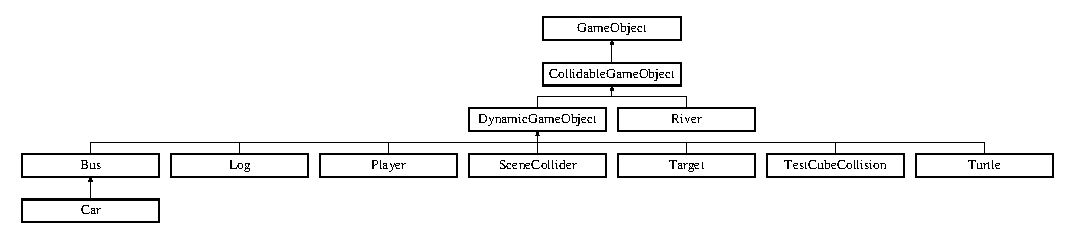
\includegraphics[height=2.758621cm]{class_collidable_game_object}
\end{center}
\end{figure}
\subsection*{Public Member Functions}
\begin{DoxyCompactItemize}
\item 
\hyperlink{class_collidable_game_object_af19a7e3e12239a38cbc076eeafcafff6}{Collidable\+Game\+Object} (\hyperlink{class_vector3}{Vector3} pos, \hyperlink{class_vector3}{Vector3} min, \hyperlink{class_vector3}{Vector3} max, \hyperlink{_game_object_8h_a57678b60d65afb213d04a6b090c64a08}{Game\+Object\+Type} type=\hyperlink{_game_object_8h_a57678b60d65afb213d04a6b090c64a08a6ce26a62afab55d7606ad4e92428b30c}{U\+N\+K\+N\+O\+WN})
\item 
virtual \hyperlink{_game_object_8h_a57678b60d65afb213d04a6b090c64a08}{Game\+Object\+Type} \hyperlink{class_collidable_game_object_a9890003d579d6318a4da31a0d540ab2f}{get\+Type} () override
\item 
virtual \hyperlink{class_bounding_box}{Bounding\+Box} \hyperlink{class_collidable_game_object_a7998e4aabd23263212e72f6a40d42036}{get\+Bounding\+Box} () const override
\item 
virtual bool \hyperlink{class_collidable_game_object_aabc837db5ee83847ad55a5f95cb106a6}{collide\+With} (const \hyperlink{class_game_object}{Game\+Object} $\ast$other) const override
\item 
virtual bool \hyperlink{class_collidable_game_object_ae972d5d27b0f9bb54e9d20f9e6c205b6}{is\+Inside\+Other} (const \hyperlink{class_game_object}{Game\+Object} $\ast$other) const
\end{DoxyCompactItemize}
\subsection*{Public Attributes}
\begin{DoxyCompactItemize}
\item 
\hyperlink{class_bounding_box}{Bounding\+Box} \hyperlink{class_collidable_game_object_a19d723799fa054bf174be196541c5f57}{bounding\+Box}
\item 
\hyperlink{_game_object_8h_a57678b60d65afb213d04a6b090c64a08}{Game\+Object\+Type} \hyperlink{class_collidable_game_object_a5c79dc25d987f169a79c2c161e1a79dd}{game\+Object\+Type}
\end{DoxyCompactItemize}
\subsection*{Additional Inherited Members}


\subsection{Constructor \& Destructor Documentation}
\mbox{\Hypertarget{class_collidable_game_object_af19a7e3e12239a38cbc076eeafcafff6}\label{class_collidable_game_object_af19a7e3e12239a38cbc076eeafcafff6}} 
\index{Collidable\+Game\+Object@{Collidable\+Game\+Object}!Collidable\+Game\+Object@{Collidable\+Game\+Object}}
\index{Collidable\+Game\+Object@{Collidable\+Game\+Object}!Collidable\+Game\+Object@{Collidable\+Game\+Object}}
\subsubsection{\texorpdfstring{Collidable\+Game\+Object()}{CollidableGameObject()}}
{\footnotesize\ttfamily Collidable\+Game\+Object\+::\+Collidable\+Game\+Object (\begin{DoxyParamCaption}\item[{\hyperlink{class_vector3}{Vector3}}]{pos,  }\item[{\hyperlink{class_vector3}{Vector3}}]{min,  }\item[{\hyperlink{class_vector3}{Vector3}}]{max,  }\item[{\hyperlink{_game_object_8h_a57678b60d65afb213d04a6b090c64a08}{Game\+Object\+Type}}]{type = {\ttfamily \hyperlink{_game_object_8h_a57678b60d65afb213d04a6b090c64a08a6ce26a62afab55d7606ad4e92428b30c}{U\+N\+K\+N\+O\+WN}} }\end{DoxyParamCaption})\hspace{0.3cm}{\ttfamily [inline]}}



\subsection{Member Function Documentation}
\mbox{\Hypertarget{class_collidable_game_object_aabc837db5ee83847ad55a5f95cb106a6}\label{class_collidable_game_object_aabc837db5ee83847ad55a5f95cb106a6}} 
\index{Collidable\+Game\+Object@{Collidable\+Game\+Object}!collide\+With@{collide\+With}}
\index{collide\+With@{collide\+With}!Collidable\+Game\+Object@{Collidable\+Game\+Object}}
\subsubsection{\texorpdfstring{collide\+With()}{collideWith()}}
{\footnotesize\ttfamily virtual bool Collidable\+Game\+Object\+::collide\+With (\begin{DoxyParamCaption}\item[{const \hyperlink{class_game_object}{Game\+Object} $\ast$}]{other }\end{DoxyParamCaption}) const\hspace{0.3cm}{\ttfamily [inline]}, {\ttfamily [override]}, {\ttfamily [virtual]}}



Reimplemented from \hyperlink{class_game_object_a9ab7d2e2beff3e91ccdc87c9fbca019e}{Game\+Object}.

\mbox{\Hypertarget{class_collidable_game_object_a7998e4aabd23263212e72f6a40d42036}\label{class_collidable_game_object_a7998e4aabd23263212e72f6a40d42036}} 
\index{Collidable\+Game\+Object@{Collidable\+Game\+Object}!get\+Bounding\+Box@{get\+Bounding\+Box}}
\index{get\+Bounding\+Box@{get\+Bounding\+Box}!Collidable\+Game\+Object@{Collidable\+Game\+Object}}
\subsubsection{\texorpdfstring{get\+Bounding\+Box()}{getBoundingBox()}}
{\footnotesize\ttfamily virtual \hyperlink{class_bounding_box}{Bounding\+Box} Collidable\+Game\+Object\+::get\+Bounding\+Box (\begin{DoxyParamCaption}{ }\end{DoxyParamCaption}) const\hspace{0.3cm}{\ttfamily [inline]}, {\ttfamily [override]}, {\ttfamily [virtual]}}



Reimplemented from \hyperlink{class_game_object_a64b37bea01266aea52a47f4a48a9cc84}{Game\+Object}.

\mbox{\Hypertarget{class_collidable_game_object_a9890003d579d6318a4da31a0d540ab2f}\label{class_collidable_game_object_a9890003d579d6318a4da31a0d540ab2f}} 
\index{Collidable\+Game\+Object@{Collidable\+Game\+Object}!get\+Type@{get\+Type}}
\index{get\+Type@{get\+Type}!Collidable\+Game\+Object@{Collidable\+Game\+Object}}
\subsubsection{\texorpdfstring{get\+Type()}{getType()}}
{\footnotesize\ttfamily virtual \hyperlink{_game_object_8h_a57678b60d65afb213d04a6b090c64a08}{Game\+Object\+Type} Collidable\+Game\+Object\+::get\+Type (\begin{DoxyParamCaption}{ }\end{DoxyParamCaption})\hspace{0.3cm}{\ttfamily [inline]}, {\ttfamily [override]}, {\ttfamily [virtual]}}



Reimplemented from \hyperlink{class_game_object_ab7ee421293a4bbe47b4102180185fbaa}{Game\+Object}.

\mbox{\Hypertarget{class_collidable_game_object_ae972d5d27b0f9bb54e9d20f9e6c205b6}\label{class_collidable_game_object_ae972d5d27b0f9bb54e9d20f9e6c205b6}} 
\index{Collidable\+Game\+Object@{Collidable\+Game\+Object}!is\+Inside\+Other@{is\+Inside\+Other}}
\index{is\+Inside\+Other@{is\+Inside\+Other}!Collidable\+Game\+Object@{Collidable\+Game\+Object}}
\subsubsection{\texorpdfstring{is\+Inside\+Other()}{isInsideOther()}}
{\footnotesize\ttfamily virtual bool Collidable\+Game\+Object\+::is\+Inside\+Other (\begin{DoxyParamCaption}\item[{const \hyperlink{class_game_object}{Game\+Object} $\ast$}]{other }\end{DoxyParamCaption}) const\hspace{0.3cm}{\ttfamily [inline]}, {\ttfamily [virtual]}}



\subsection{Member Data Documentation}
\mbox{\Hypertarget{class_collidable_game_object_a19d723799fa054bf174be196541c5f57}\label{class_collidable_game_object_a19d723799fa054bf174be196541c5f57}} 
\index{Collidable\+Game\+Object@{Collidable\+Game\+Object}!bounding\+Box@{bounding\+Box}}
\index{bounding\+Box@{bounding\+Box}!Collidable\+Game\+Object@{Collidable\+Game\+Object}}
\subsubsection{\texorpdfstring{bounding\+Box}{boundingBox}}
{\footnotesize\ttfamily \hyperlink{class_bounding_box}{Bounding\+Box} Collidable\+Game\+Object\+::bounding\+Box}

\mbox{\Hypertarget{class_collidable_game_object_a5c79dc25d987f169a79c2c161e1a79dd}\label{class_collidable_game_object_a5c79dc25d987f169a79c2c161e1a79dd}} 
\index{Collidable\+Game\+Object@{Collidable\+Game\+Object}!game\+Object\+Type@{game\+Object\+Type}}
\index{game\+Object\+Type@{game\+Object\+Type}!Collidable\+Game\+Object@{Collidable\+Game\+Object}}
\subsubsection{\texorpdfstring{game\+Object\+Type}{gameObjectType}}
{\footnotesize\ttfamily \hyperlink{_game_object_8h_a57678b60d65afb213d04a6b090c64a08}{Game\+Object\+Type} Collidable\+Game\+Object\+::game\+Object\+Type}



The documentation for this class was generated from the following file\+:\begin{DoxyCompactItemize}
\item 
/\+Users/matya/\+A\+V\+T7/src/\hyperlink{_collidable_game_object_8h}{Collidable\+Game\+Object.\+h}\end{DoxyCompactItemize}

\hypertarget{class_coordinates}{}\section{Coordinates Class Reference}
\label{class_coordinates}\index{Coordinates@{Coordinates}}


{\ttfamily \#include $<$Coordinates.\+h$>$}

Inheritance diagram for Coordinates\+:\begin{figure}[H]
\begin{center}
\leavevmode
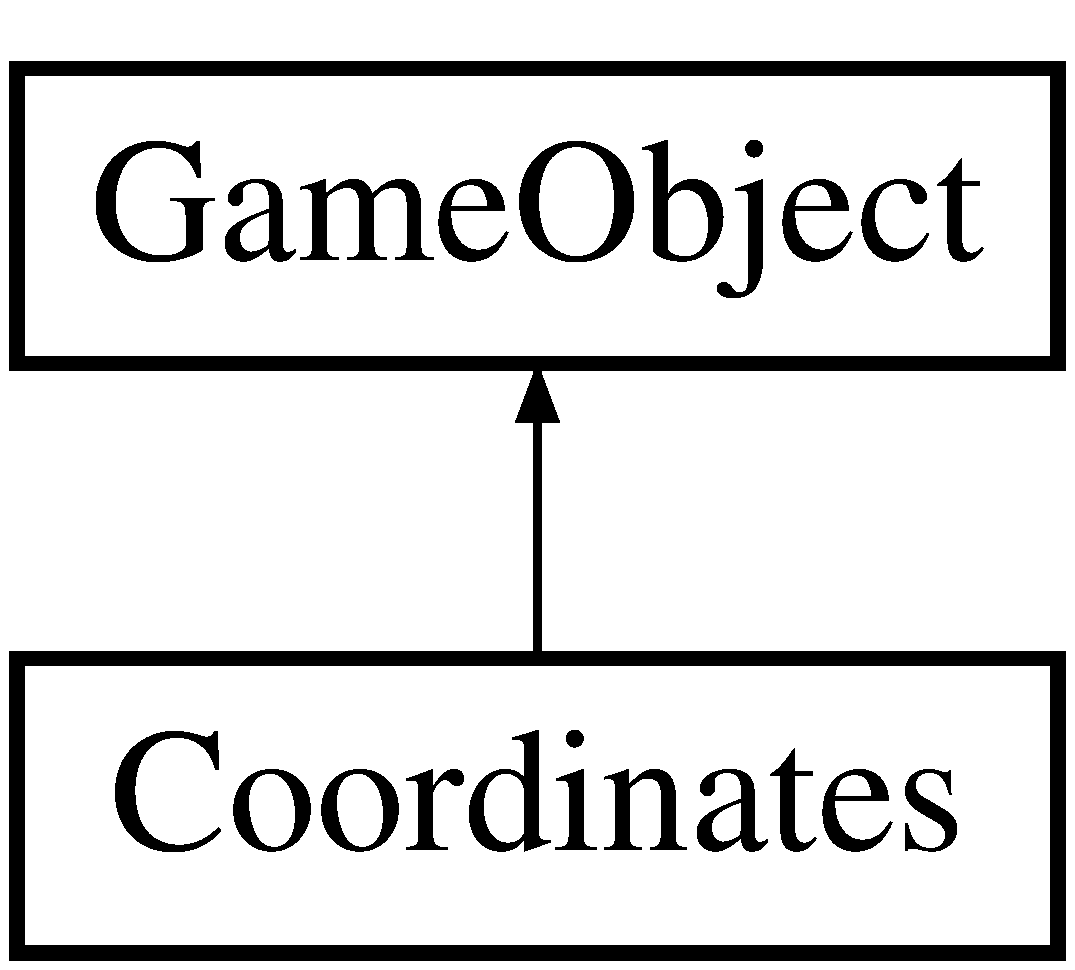
\includegraphics[height=2.000000cm]{class_coordinates}
\end{center}
\end{figure}
\subsection*{Public Member Functions}
\begin{DoxyCompactItemize}
\item 
\hyperlink{class_coordinates_a1491cf3cc0f7281978bd289a2100a16c}{Coordinates} (\hyperlink{class_vector3}{Vector3} pos)
\item 
void \hyperlink{class_coordinates_aaadf934b8f184a9e0abe504e4c2da9b1}{init} () override
\item 
void \hyperlink{class_coordinates_afa2d40b313b3b2933f9030ebfbe31045}{render} () override
\end{DoxyCompactItemize}
\subsection*{Additional Inherited Members}


\subsection{Constructor \& Destructor Documentation}
\mbox{\Hypertarget{class_coordinates_a1491cf3cc0f7281978bd289a2100a16c}\label{class_coordinates_a1491cf3cc0f7281978bd289a2100a16c}} 
\index{Coordinates@{Coordinates}!Coordinates@{Coordinates}}
\index{Coordinates@{Coordinates}!Coordinates@{Coordinates}}
\subsubsection{\texorpdfstring{Coordinates()}{Coordinates()}}
{\footnotesize\ttfamily Coordinates\+::\+Coordinates (\begin{DoxyParamCaption}\item[{\hyperlink{class_vector3}{Vector3}}]{pos }\end{DoxyParamCaption})\hspace{0.3cm}{\ttfamily [inline]}}



\subsection{Member Function Documentation}
\mbox{\Hypertarget{class_coordinates_aaadf934b8f184a9e0abe504e4c2da9b1}\label{class_coordinates_aaadf934b8f184a9e0abe504e4c2da9b1}} 
\index{Coordinates@{Coordinates}!init@{init}}
\index{init@{init}!Coordinates@{Coordinates}}
\subsubsection{\texorpdfstring{init()}{init()}}
{\footnotesize\ttfamily void Coordinates\+::init (\begin{DoxyParamCaption}{ }\end{DoxyParamCaption})\hspace{0.3cm}{\ttfamily [inline]}, {\ttfamily [override]}, {\ttfamily [virtual]}}



Reimplemented from \hyperlink{class_game_object_aecb2c1b9f69715d854f7604d5d7978ec}{Game\+Object}.

\mbox{\Hypertarget{class_coordinates_afa2d40b313b3b2933f9030ebfbe31045}\label{class_coordinates_afa2d40b313b3b2933f9030ebfbe31045}} 
\index{Coordinates@{Coordinates}!render@{render}}
\index{render@{render}!Coordinates@{Coordinates}}
\subsubsection{\texorpdfstring{render()}{render()}}
{\footnotesize\ttfamily void Coordinates\+::render (\begin{DoxyParamCaption}{ }\end{DoxyParamCaption})\hspace{0.3cm}{\ttfamily [inline]}, {\ttfamily [override]}, {\ttfamily [virtual]}}



Reimplemented from \hyperlink{class_game_object_a484efb66a7a27c101e84c11d9905d7a6}{Game\+Object}.



The documentation for this class was generated from the following file\+:\begin{DoxyCompactItemize}
\item 
/\+Users/matya/\+A\+V\+T7/src/objects/\hyperlink{_coordinates_8h}{Coordinates.\+h}\end{DoxyCompactItemize}

\hypertarget{class_directional_light}{}\section{Directional\+Light Class Reference}
\label{class_directional_light}\index{Directional\+Light@{Directional\+Light}}


{\ttfamily \#include $<$Directional\+Light.\+h$>$}

Inheritance diagram for Directional\+Light\+:\begin{figure}[H]
\begin{center}
\leavevmode
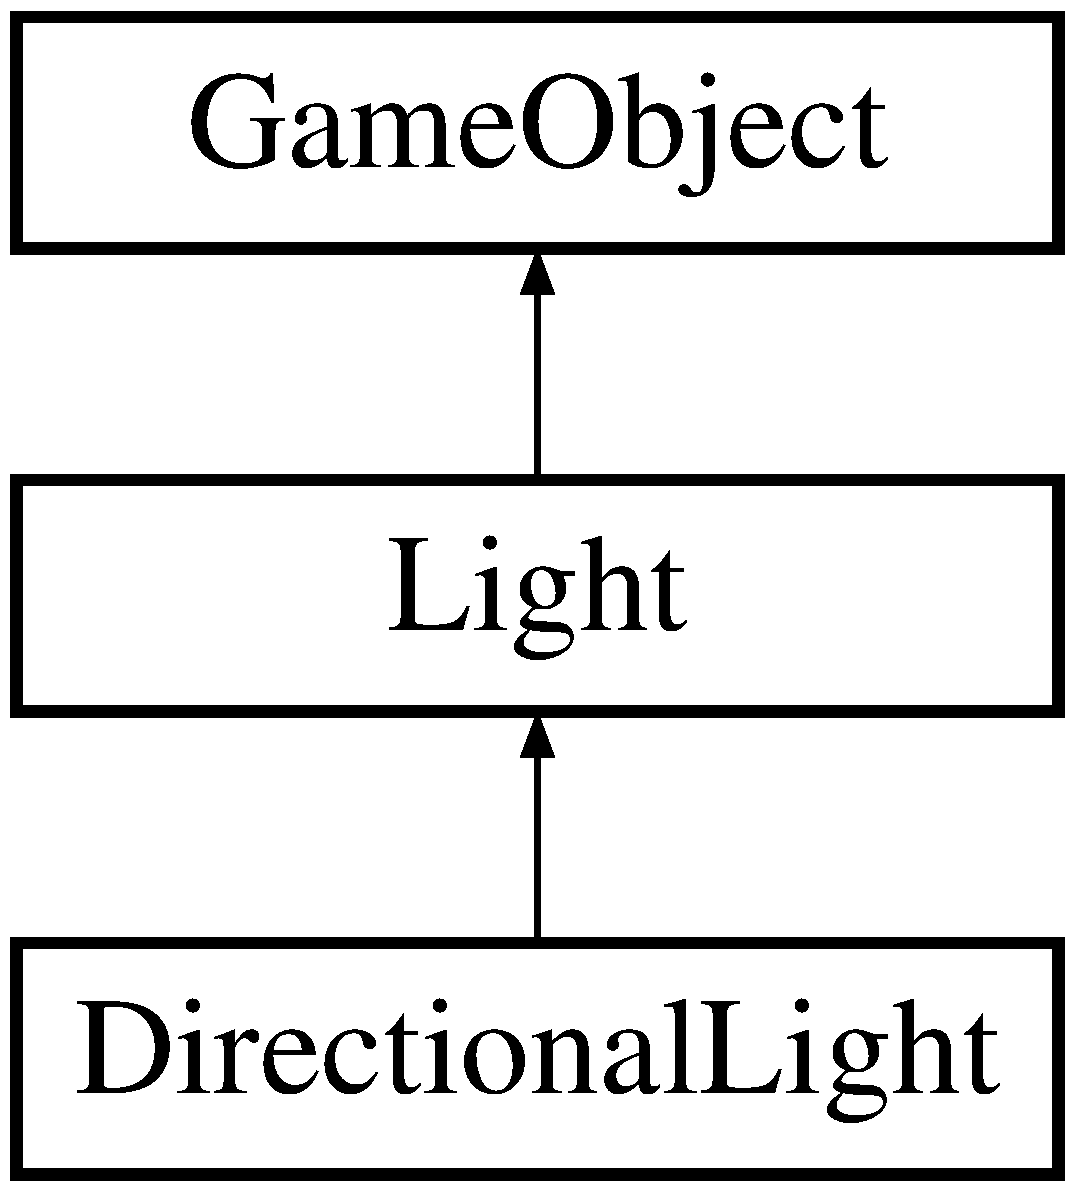
\includegraphics[height=3.000000cm]{class_directional_light}
\end{center}
\end{figure}
\subsection*{Public Member Functions}
\begin{DoxyCompactItemize}
\item 
\hyperlink{class_directional_light_a15e97766ae5a5fdd50c9429a79d37292}{Directional\+Light} (\hyperlink{class_vector3}{Vector3} pos, int \hyperlink{class_light_ae0028340ad3a9f2e196b68365d5fe972}{light\+\_\+id}, bool light\+\_\+active=true)
\item 
void \hyperlink{class_directional_light_aa56c9af208dd1bc66967d219297b6e67}{render} () final
\end{DoxyCompactItemize}
\subsection*{Additional Inherited Members}


\subsection{Constructor \& Destructor Documentation}
\mbox{\Hypertarget{class_directional_light_a15e97766ae5a5fdd50c9429a79d37292}\label{class_directional_light_a15e97766ae5a5fdd50c9429a79d37292}} 
\index{Directional\+Light@{Directional\+Light}!Directional\+Light@{Directional\+Light}}
\index{Directional\+Light@{Directional\+Light}!Directional\+Light@{Directional\+Light}}
\subsubsection{\texorpdfstring{Directional\+Light()}{DirectionalLight()}}
{\footnotesize\ttfamily Directional\+Light\+::\+Directional\+Light (\begin{DoxyParamCaption}\item[{\hyperlink{class_vector3}{Vector3}}]{pos,  }\item[{int}]{light\+\_\+id,  }\item[{bool}]{light\+\_\+active = {\ttfamily true} }\end{DoxyParamCaption})\hspace{0.3cm}{\ttfamily [inline]}}



\subsection{Member Function Documentation}
\mbox{\Hypertarget{class_directional_light_aa56c9af208dd1bc66967d219297b6e67}\label{class_directional_light_aa56c9af208dd1bc66967d219297b6e67}} 
\index{Directional\+Light@{Directional\+Light}!render@{render}}
\index{render@{render}!Directional\+Light@{Directional\+Light}}
\subsubsection{\texorpdfstring{render()}{render()}}
{\footnotesize\ttfamily void Directional\+Light\+::render (\begin{DoxyParamCaption}{ }\end{DoxyParamCaption})\hspace{0.3cm}{\ttfamily [inline]}, {\ttfamily [final]}, {\ttfamily [virtual]}}



Reimplemented from \hyperlink{class_game_object_a484efb66a7a27c101e84c11d9905d7a6}{Game\+Object}.



The documentation for this class was generated from the following file\+:\begin{DoxyCompactItemize}
\item 
/\+Users/matya/\+A\+V\+T7/src/objects/\hyperlink{_directional_light_8h}{Directional\+Light.\+h}\end{DoxyCompactItemize}

\hypertarget{class_dynamic_game_object}{}\section{Dynamic\+Game\+Object Class Reference}
\label{class_dynamic_game_object}\index{Dynamic\+Game\+Object@{Dynamic\+Game\+Object}}


{\ttfamily \#include $<$Dynamic\+Game\+Object.\+h$>$}

Inheritance diagram for Dynamic\+Game\+Object\+:\begin{figure}[H]
\begin{center}
\leavevmode
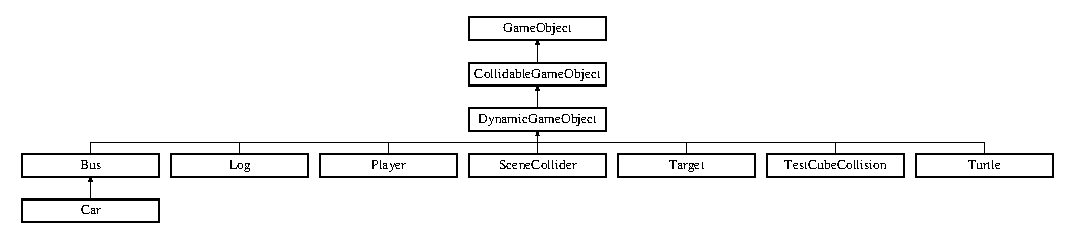
\includegraphics[height=2.758621cm]{class_dynamic_game_object}
\end{center}
\end{figure}
\subsection*{Public Member Functions}
\begin{DoxyCompactItemize}
\item 
\hyperlink{class_dynamic_game_object_ab7d7036c283760e0035d39713a82016a}{Dynamic\+Game\+Object} (\hyperlink{class_vector3}{Vector3} pos, \hyperlink{class_vector3}{Vector3} min, \hyperlink{class_vector3}{Vector3} max, \hyperlink{_game_object_8h_a57678b60d65afb213d04a6b090c64a08}{Game\+Object\+Type} type, \hyperlink{class_vector3}{Vector3} \hyperlink{class_dynamic_game_object_a54cb8a3a5fe8314cd5751f223b2b49ae}{speed})
\item 
\hyperlink{class_vector3}{Vector3} \hyperlink{class_dynamic_game_object_a22d2cededc50901db950ac23b46e4d42}{get\+Speed} () final
\item 
void \hyperlink{class_dynamic_game_object_aaa505b57d131bbbce44d500ec2ca0e83}{update} (int \hyperlink{_game_manager_8h_afea6a95c7a1c119b7106a4c735eb259d}{delta\+Time}) override
\item 
virtual float \hyperlink{class_dynamic_game_object_a677f4bdcd11800fee831a13234382619}{get\+Speed\+Multiplier} () const
\item 
virtual void \hyperlink{class_dynamic_game_object_a7bf254357b0d2491044d175afdc36ca4}{set\+Speed\+Multiplier} (float new\+Speed\+Mult)
\end{DoxyCompactItemize}
\subsection*{Public Attributes}
\begin{DoxyCompactItemize}
\item 
\hyperlink{class_vector3}{Vector3} \hyperlink{class_dynamic_game_object_a54cb8a3a5fe8314cd5751f223b2b49ae}{speed}
\item 
\hyperlink{class_vector3}{Vector3} \hyperlink{class_dynamic_game_object_a43bcea908ce101c1060dfec7eb3099a9}{init\+Speed}
\item 
\hyperlink{class_vector3}{Vector3} \hyperlink{class_dynamic_game_object_a3bb99e52ae5e37dd3b309e80c2262c82}{init\+Pos}
\item 
float \hyperlink{class_dynamic_game_object_a0816663ea0effab6d4b441600aa38b59}{environment\+Speed\+Multiplier} = 1.\+0f
\end{DoxyCompactItemize}
\subsection*{Additional Inherited Members}


\subsection{Constructor \& Destructor Documentation}
\mbox{\Hypertarget{class_dynamic_game_object_ab7d7036c283760e0035d39713a82016a}\label{class_dynamic_game_object_ab7d7036c283760e0035d39713a82016a}} 
\index{Dynamic\+Game\+Object@{Dynamic\+Game\+Object}!Dynamic\+Game\+Object@{Dynamic\+Game\+Object}}
\index{Dynamic\+Game\+Object@{Dynamic\+Game\+Object}!Dynamic\+Game\+Object@{Dynamic\+Game\+Object}}
\subsubsection{\texorpdfstring{Dynamic\+Game\+Object()}{DynamicGameObject()}}
{\footnotesize\ttfamily Dynamic\+Game\+Object\+::\+Dynamic\+Game\+Object (\begin{DoxyParamCaption}\item[{\hyperlink{class_vector3}{Vector3}}]{pos,  }\item[{\hyperlink{class_vector3}{Vector3}}]{min,  }\item[{\hyperlink{class_vector3}{Vector3}}]{max,  }\item[{\hyperlink{_game_object_8h_a57678b60d65afb213d04a6b090c64a08}{Game\+Object\+Type}}]{type,  }\item[{\hyperlink{class_vector3}{Vector3}}]{speed }\end{DoxyParamCaption})\hspace{0.3cm}{\ttfamily [inline]}}



\subsection{Member Function Documentation}
\mbox{\Hypertarget{class_dynamic_game_object_a22d2cededc50901db950ac23b46e4d42}\label{class_dynamic_game_object_a22d2cededc50901db950ac23b46e4d42}} 
\index{Dynamic\+Game\+Object@{Dynamic\+Game\+Object}!get\+Speed@{get\+Speed}}
\index{get\+Speed@{get\+Speed}!Dynamic\+Game\+Object@{Dynamic\+Game\+Object}}
\subsubsection{\texorpdfstring{get\+Speed()}{getSpeed()}}
{\footnotesize\ttfamily \hyperlink{class_vector3}{Vector3} Dynamic\+Game\+Object\+::get\+Speed (\begin{DoxyParamCaption}{ }\end{DoxyParamCaption})\hspace{0.3cm}{\ttfamily [inline]}, {\ttfamily [final]}, {\ttfamily [virtual]}}



Reimplemented from \hyperlink{class_game_object_ac08043ba5563ecbd118e522169f7f919}{Game\+Object}.

\mbox{\Hypertarget{class_dynamic_game_object_a677f4bdcd11800fee831a13234382619}\label{class_dynamic_game_object_a677f4bdcd11800fee831a13234382619}} 
\index{Dynamic\+Game\+Object@{Dynamic\+Game\+Object}!get\+Speed\+Multiplier@{get\+Speed\+Multiplier}}
\index{get\+Speed\+Multiplier@{get\+Speed\+Multiplier}!Dynamic\+Game\+Object@{Dynamic\+Game\+Object}}
\subsubsection{\texorpdfstring{get\+Speed\+Multiplier()}{getSpeedMultiplier()}}
{\footnotesize\ttfamily virtual float Dynamic\+Game\+Object\+::get\+Speed\+Multiplier (\begin{DoxyParamCaption}{ }\end{DoxyParamCaption}) const\hspace{0.3cm}{\ttfamily [inline]}, {\ttfamily [virtual]}}



Reimplemented from \hyperlink{class_game_object_a577ca32504b1551f75e1724219c4f6cf}{Game\+Object}.

\mbox{\Hypertarget{class_dynamic_game_object_a7bf254357b0d2491044d175afdc36ca4}\label{class_dynamic_game_object_a7bf254357b0d2491044d175afdc36ca4}} 
\index{Dynamic\+Game\+Object@{Dynamic\+Game\+Object}!set\+Speed\+Multiplier@{set\+Speed\+Multiplier}}
\index{set\+Speed\+Multiplier@{set\+Speed\+Multiplier}!Dynamic\+Game\+Object@{Dynamic\+Game\+Object}}
\subsubsection{\texorpdfstring{set\+Speed\+Multiplier()}{setSpeedMultiplier()}}
{\footnotesize\ttfamily virtual void Dynamic\+Game\+Object\+::set\+Speed\+Multiplier (\begin{DoxyParamCaption}\item[{float}]{new\+Speed\+Mult }\end{DoxyParamCaption})\hspace{0.3cm}{\ttfamily [inline]}, {\ttfamily [virtual]}}



Reimplemented from \hyperlink{class_game_object_ab3d0617433250c19ccbb64bfca1bb905}{Game\+Object}.



Reimplemented in \hyperlink{class_player_a9098e6b411ea9102b02bb911eca6515b}{Player}.

\mbox{\Hypertarget{class_dynamic_game_object_aaa505b57d131bbbce44d500ec2ca0e83}\label{class_dynamic_game_object_aaa505b57d131bbbce44d500ec2ca0e83}} 
\index{Dynamic\+Game\+Object@{Dynamic\+Game\+Object}!update@{update}}
\index{update@{update}!Dynamic\+Game\+Object@{Dynamic\+Game\+Object}}
\subsubsection{\texorpdfstring{update()}{update()}}
{\footnotesize\ttfamily void Dynamic\+Game\+Object\+::update (\begin{DoxyParamCaption}\item[{int}]{delta\+Time }\end{DoxyParamCaption})\hspace{0.3cm}{\ttfamily [inline]}, {\ttfamily [override]}, {\ttfamily [virtual]}}



Reimplemented from \hyperlink{class_game_object_a6dc5215a3d0efc7a9e2332006b31c868}{Game\+Object}.



Reimplemented in \hyperlink{class_turtle_a6d62e3f4e21f5ce3ffb4e7e2a8a9da1b}{Turtle}, \hyperlink{class_player_a51e705a6ad3628144e02832d1839b360}{Player}, \hyperlink{class_bus_ad07157ce2a50211ea599d040da7a4517}{Bus}, \hyperlink{class_test_cube_collision_ae528ac632377372d93964c938748fddf}{Test\+Cube\+Collision}, and \hyperlink{class_target_a5f3b2dc70e8065e53199ab3244059ba7}{Target}.



\subsection{Member Data Documentation}
\mbox{\Hypertarget{class_dynamic_game_object_a0816663ea0effab6d4b441600aa38b59}\label{class_dynamic_game_object_a0816663ea0effab6d4b441600aa38b59}} 
\index{Dynamic\+Game\+Object@{Dynamic\+Game\+Object}!environment\+Speed\+Multiplier@{environment\+Speed\+Multiplier}}
\index{environment\+Speed\+Multiplier@{environment\+Speed\+Multiplier}!Dynamic\+Game\+Object@{Dynamic\+Game\+Object}}
\subsubsection{\texorpdfstring{environment\+Speed\+Multiplier}{environmentSpeedMultiplier}}
{\footnotesize\ttfamily float Dynamic\+Game\+Object\+::environment\+Speed\+Multiplier = 1.\+0f}

\mbox{\Hypertarget{class_dynamic_game_object_a3bb99e52ae5e37dd3b309e80c2262c82}\label{class_dynamic_game_object_a3bb99e52ae5e37dd3b309e80c2262c82}} 
\index{Dynamic\+Game\+Object@{Dynamic\+Game\+Object}!init\+Pos@{init\+Pos}}
\index{init\+Pos@{init\+Pos}!Dynamic\+Game\+Object@{Dynamic\+Game\+Object}}
\subsubsection{\texorpdfstring{init\+Pos}{initPos}}
{\footnotesize\ttfamily \hyperlink{class_vector3}{Vector3} Dynamic\+Game\+Object\+::init\+Pos}

\mbox{\Hypertarget{class_dynamic_game_object_a43bcea908ce101c1060dfec7eb3099a9}\label{class_dynamic_game_object_a43bcea908ce101c1060dfec7eb3099a9}} 
\index{Dynamic\+Game\+Object@{Dynamic\+Game\+Object}!init\+Speed@{init\+Speed}}
\index{init\+Speed@{init\+Speed}!Dynamic\+Game\+Object@{Dynamic\+Game\+Object}}
\subsubsection{\texorpdfstring{init\+Speed}{initSpeed}}
{\footnotesize\ttfamily \hyperlink{class_vector3}{Vector3} Dynamic\+Game\+Object\+::init\+Speed}

\mbox{\Hypertarget{class_dynamic_game_object_a54cb8a3a5fe8314cd5751f223b2b49ae}\label{class_dynamic_game_object_a54cb8a3a5fe8314cd5751f223b2b49ae}} 
\index{Dynamic\+Game\+Object@{Dynamic\+Game\+Object}!speed@{speed}}
\index{speed@{speed}!Dynamic\+Game\+Object@{Dynamic\+Game\+Object}}
\subsubsection{\texorpdfstring{speed}{speed}}
{\footnotesize\ttfamily \hyperlink{class_vector3}{Vector3} Dynamic\+Game\+Object\+::speed}



The documentation for this class was generated from the following file\+:\begin{DoxyCompactItemize}
\item 
/\+Users/matya/\+A\+V\+T7/src/\hyperlink{_dynamic_game_object_8h}{Dynamic\+Game\+Object.\+h}\end{DoxyCompactItemize}

\hypertarget{class_game_manager}{}\section{Game\+Manager Class Reference}
\label{class_game_manager}\index{Game\+Manager@{Game\+Manager}}


{\ttfamily \#include $<$Game\+Manager.\+h$>$}

\subsection*{Public Types}
\begin{DoxyCompactItemize}
\item 
enum \hyperlink{class_game_manager_a3f3a18cdc6b3c7c7565927e895eea247}{Camera\+Type} \{ \hyperlink{class_game_manager_a3f3a18cdc6b3c7c7565927e895eea247a2e83b11bc593230f7f30214b50fd6cae}{C\+A\+M\+E\+R\+A\+\_\+\+P\+E\+R\+S\+P\+E\+C\+T\+I\+V\+E\+\_\+\+F\+O\+L\+L\+OW}, 
\hyperlink{class_game_manager_a3f3a18cdc6b3c7c7565927e895eea247a1bdebab59d48229c3066fa423ca789cc}{C\+A\+M\+E\+R\+A\+\_\+\+P\+E\+R\+S\+P\+E\+C\+T\+I\+V\+E\+\_\+\+F\+I\+X\+ED}, 
\hyperlink{class_game_manager_a3f3a18cdc6b3c7c7565927e895eea247a767d4e04d0898c8eb3f53a3b25be0194}{C\+A\+M\+E\+R\+A\+\_\+\+O\+R\+T\+HO}
 \}
\end{DoxyCompactItemize}
\subsection*{Public Member Functions}
\begin{DoxyCompactItemize}
\item 
\hyperlink{class_game_manager_aa0e2424dc1a39d380e5b6605b179bf05}{Game\+Manager} ()
\item 
void \hyperlink{class_game_manager_a7552e5b78753f1e78847ef1ac7bd0596}{change\+Size} (int w, int h)
\item 
void \hyperlink{class_game_manager_a1d22955ef38d38ee720432a0d56f33ae}{process\+Keys} (unsigned char key, int xx, int yy)
\item 
void \hyperlink{class_game_manager_ae51ce09e93fed12b8e45d6669c3975cd}{move\+Player} (float x, float z)
\item 
G\+Luint \hyperlink{class_game_manager_a88396466f77d0013a1bb085a6d19aad8}{setup\+Shaders} ()
\item 
void \hyperlink{class_game_manager_af98f6eb4ebe36b9405700cc95a6771be}{init\+Scene} ()
\item 
void \hyperlink{class_game_manager_aef819f3b139bc195db44a49299768eee}{render\+Scene} ()
\end{DoxyCompactItemize}
\subsection*{Public Attributes}
\begin{DoxyCompactItemize}
\item 
G\+Lint \hyperlink{class_game_manager_a7292d1f46ee4141dbb1b6a7a8cc134f2}{Window\+Handle} = 0
\item 
G\+Lint \hyperlink{class_game_manager_a0d7672e0e14f75901291a62862d7eb60}{Frame\+Count} = 0
\item 
string \hyperlink{class_game_manager_a8e65d4c5dca91cb6af25bf6c25d2a009}{info\+String} = \char`\"{}\char`\"{}
\item 
bool \hyperlink{class_game_manager_a8faf5fabfe8174f79f449b60065b8048}{is\+Playing} = true
\item 
int \hyperlink{class_game_manager_aceb9f59354267d31fc6dfb023a695854}{score} = 0
\item 
int \hyperlink{class_game_manager_ab2ed8869ac478caf69ea29e6de26ea80}{points\+Per\+Target} = 100
\item 
float \hyperlink{class_game_manager_ac6d13a816358fd7c754f4ef1fb82f7e4}{speed\+Multiplier} = 1.\+2f
\item 
const float \hyperlink{class_game_manager_a34e763c41e51dccf7241b784de62e381}{top\+Vertical\+Limit\+Player\+Pos} = -\/6.\+0f
\item 
const float \hyperlink{class_game_manager_aac2d3978ba280076a75ba8863c2da9ac}{bottom\+Vertical\+Limit\+Player\+Pos} = 6.\+0f
\item 
const float \hyperlink{class_game_manager_af27090b5d1db50311f0453de5df095bc}{left\+Horizontal\+Limit\+Player\+Pos} = -\/6.\+0f
\item 
const float \hyperlink{class_game_manager_ad0bc4e5fd9c85e9b25bd4579a508151f}{right\+Horizontal\+Limit\+Player\+Pos} = 6.\+0f
\item 
vector$<$ \hyperlink{class_game_object}{Game\+Object} $\ast$ $>$ \hyperlink{class_game_manager_a8b02c0a19f162a651041cddb4821a82c}{game\+Objects} = vector$<$\hyperlink{class_game_object}{Game\+Object}$\ast$$>$()
\item 
vector$<$ \hyperlink{class_bus}{Bus} $\ast$ $>$ \hyperlink{class_game_manager_aaca42616afec776da2bf0ccd0641f8e0}{busses} = vector$<$\hyperlink{class_bus}{Bus}$\ast$$>$()
\item 
vector$<$ \hyperlink{class_car}{Car} $\ast$ $>$ \hyperlink{class_game_manager_af6d97ab7a3c0df3c4999aa60c7dcc083}{cars} = vector$<$\hyperlink{class_car}{Car}$\ast$$>$()
\item 
vector$<$ \hyperlink{class_log}{Log} $\ast$ $>$ \hyperlink{class_game_manager_a02676ea2e67ce2773e32844ac2ffc64e}{logs} = vector$<$\hyperlink{class_log}{Log}$\ast$$>$()
\item 
vector$<$ \hyperlink{class_turtle}{Turtle} $\ast$ $>$ \hyperlink{class_game_manager_a47719947c503583906c085b293759de2}{turtles} = vector$<$\hyperlink{class_turtle}{Turtle}$\ast$$>$()
\item 
G\+Lint \hyperlink{class_game_manager_a6e1ed3a2dc585e518b007abebd0a8fdc}{last\+Move\+Time} = 0
\item 
G\+Lint \hyperlink{class_game_manager_adce6a582e4f8ddaa5d341d2ba91e551a}{move\+Timeout} = 300
\item 
\hyperlink{class_game_manager_a3f3a18cdc6b3c7c7565927e895eea247}{Camera\+Type} \hyperlink{class_game_manager_a9384497e205b12a342442aae07d729b5}{current\+Camera\+Type} = \hyperlink{class_game_manager_a3f3a18cdc6b3c7c7565927e895eea247a2e83b11bc593230f7f30214b50fd6cae}{C\+A\+M\+E\+R\+A\+\_\+\+P\+E\+R\+S\+P\+E\+C\+T\+I\+V\+E\+\_\+\+F\+O\+L\+L\+OW}
\item 
\hyperlink{class_camera_perspective_moving}{Camera\+Perspective\+Moving} \hyperlink{class_game_manager_acc870ff353939b5b7970e85d536b10c7}{camera\+Perspective\+Moving} = \hyperlink{class_camera_perspective_moving}{Camera\+Perspective\+Moving}(20, 0, 40, \hyperlink{class_vector3}{Vector3}(0, 20, 0))
\item 
\hyperlink{class_camera_perspective}{Camera\+Perspective} \hyperlink{class_game_manager_a06fd04f0626f7ff640804e4506fa6015}{camera\+Perspective\+Fixed} = \hyperlink{class_camera_perspective}{Camera\+Perspective}(20, 0, 90, \hyperlink{class_vector3}{Vector3}(0, 20, 0))
\item 
\hyperlink{class_camera_orthogonal}{Camera\+Orthogonal} \hyperlink{class_game_manager_a151b31ac1969c0e3723b7aec3a20c4b0}{camera\+Orthogonal} = \hyperlink{class_camera_orthogonal}{Camera\+Orthogonal}(-\/7, 8, -\/8, 7)
\item 
\hyperlink{class_player}{Player} $\ast$ \hyperlink{class_game_manager_a22f47dea61789d0a10d9967d9084c5d9}{player} = new \hyperlink{class_player}{Player}(\hyperlink{class_vector3}{Vector3}(-\/5.\+0f, 1, 0))
\item 
\hyperlink{class_scene_collider}{Scene\+Collider} $\ast$ \hyperlink{class_game_manager_acc9cc8586b0c42ac76ffccfbb7b6aaa6}{scene\+Collider} = new \hyperlink{class_scene_collider}{Scene\+Collider}(\hyperlink{class_vector3}{Vector3}(-\/6.\+0f, -\/1, -\/6))
\item 
\hyperlink{class_target}{Target} $\ast$ \hyperlink{class_game_manager_a4989ddffb424aa668ac66107e6a0eb6f}{target} = new \hyperlink{class_target}{Target}(\hyperlink{class_vector3}{Vector3}(0.\+25f, 1.\+25f, -\/5.\+75f))
\item 
\hyperlink{class_light}{Light} $\ast$ \hyperlink{class_game_manager_a61953f70df310072a821385a7f768f99}{directional\+Light} = new \hyperlink{class_directional_light}{Directional\+Light}(\hyperlink{class_vector3}{Vector3}(0.\+0f, 5.\+0f, 0.\+0f), 6, false)
\item 
\hyperlink{class_spot_light}{Spot\+Light} $\ast$ \hyperlink{class_game_manager_a88429d344ac8ceb5a5a65ccc86105655}{spot\+Light} = new \hyperlink{class_spot_light}{Spot\+Light}(\hyperlink{class_vector3}{Vector3}(0, -\/1, 0), \hyperlink{class_vector3}{Vector3}(0, 2, 0), 7, false)
\item 
vector$<$ \hyperlink{class_point_light}{Point\+Light} $\ast$ $>$ \hyperlink{class_game_manager_a67b33597f0667606cbcf088f8381df10}{point\+Lights} = vector$<$\hyperlink{class_point_light}{Point\+Light}$\ast$$>$()
\end{DoxyCompactItemize}


\subsection{Member Enumeration Documentation}
\mbox{\Hypertarget{class_game_manager_a3f3a18cdc6b3c7c7565927e895eea247}\label{class_game_manager_a3f3a18cdc6b3c7c7565927e895eea247}} 
\index{Game\+Manager@{Game\+Manager}!Camera\+Type@{Camera\+Type}}
\index{Camera\+Type@{Camera\+Type}!Game\+Manager@{Game\+Manager}}
\subsubsection{\texorpdfstring{Camera\+Type}{CameraType}}
{\footnotesize\ttfamily enum \hyperlink{class_game_manager_a3f3a18cdc6b3c7c7565927e895eea247}{Game\+Manager\+::\+Camera\+Type}}

\begin{DoxyEnumFields}{Enumerator}
\raisebox{\heightof{T}}[0pt][0pt]{\index{C\+A\+M\+E\+R\+A\+\_\+\+P\+E\+R\+S\+P\+E\+C\+T\+I\+V\+E\+\_\+\+F\+O\+L\+L\+OW@{C\+A\+M\+E\+R\+A\+\_\+\+P\+E\+R\+S\+P\+E\+C\+T\+I\+V\+E\+\_\+\+F\+O\+L\+L\+OW}!Game\+Manager@{Game\+Manager}}\index{Game\+Manager@{Game\+Manager}!C\+A\+M\+E\+R\+A\+\_\+\+P\+E\+R\+S\+P\+E\+C\+T\+I\+V\+E\+\_\+\+F\+O\+L\+L\+OW@{C\+A\+M\+E\+R\+A\+\_\+\+P\+E\+R\+S\+P\+E\+C\+T\+I\+V\+E\+\_\+\+F\+O\+L\+L\+OW}}}\mbox{\Hypertarget{class_game_manager_a3f3a18cdc6b3c7c7565927e895eea247a2e83b11bc593230f7f30214b50fd6cae}\label{class_game_manager_a3f3a18cdc6b3c7c7565927e895eea247a2e83b11bc593230f7f30214b50fd6cae}} 
C\+A\+M\+E\+R\+A\+\_\+\+P\+E\+R\+S\+P\+E\+C\+T\+I\+V\+E\+\_\+\+F\+O\+L\+L\+OW&\\
\hline

\raisebox{\heightof{T}}[0pt][0pt]{\index{C\+A\+M\+E\+R\+A\+\_\+\+P\+E\+R\+S\+P\+E\+C\+T\+I\+V\+E\+\_\+\+F\+I\+X\+ED@{C\+A\+M\+E\+R\+A\+\_\+\+P\+E\+R\+S\+P\+E\+C\+T\+I\+V\+E\+\_\+\+F\+I\+X\+ED}!Game\+Manager@{Game\+Manager}}\index{Game\+Manager@{Game\+Manager}!C\+A\+M\+E\+R\+A\+\_\+\+P\+E\+R\+S\+P\+E\+C\+T\+I\+V\+E\+\_\+\+F\+I\+X\+ED@{C\+A\+M\+E\+R\+A\+\_\+\+P\+E\+R\+S\+P\+E\+C\+T\+I\+V\+E\+\_\+\+F\+I\+X\+ED}}}\mbox{\Hypertarget{class_game_manager_a3f3a18cdc6b3c7c7565927e895eea247a1bdebab59d48229c3066fa423ca789cc}\label{class_game_manager_a3f3a18cdc6b3c7c7565927e895eea247a1bdebab59d48229c3066fa423ca789cc}} 
C\+A\+M\+E\+R\+A\+\_\+\+P\+E\+R\+S\+P\+E\+C\+T\+I\+V\+E\+\_\+\+F\+I\+X\+ED&\\
\hline

\raisebox{\heightof{T}}[0pt][0pt]{\index{C\+A\+M\+E\+R\+A\+\_\+\+O\+R\+T\+HO@{C\+A\+M\+E\+R\+A\+\_\+\+O\+R\+T\+HO}!Game\+Manager@{Game\+Manager}}\index{Game\+Manager@{Game\+Manager}!C\+A\+M\+E\+R\+A\+\_\+\+O\+R\+T\+HO@{C\+A\+M\+E\+R\+A\+\_\+\+O\+R\+T\+HO}}}\mbox{\Hypertarget{class_game_manager_a3f3a18cdc6b3c7c7565927e895eea247a767d4e04d0898c8eb3f53a3b25be0194}\label{class_game_manager_a3f3a18cdc6b3c7c7565927e895eea247a767d4e04d0898c8eb3f53a3b25be0194}} 
C\+A\+M\+E\+R\+A\+\_\+\+O\+R\+T\+HO&\\
\hline

\end{DoxyEnumFields}


\subsection{Constructor \& Destructor Documentation}
\mbox{\Hypertarget{class_game_manager_aa0e2424dc1a39d380e5b6605b179bf05}\label{class_game_manager_aa0e2424dc1a39d380e5b6605b179bf05}} 
\index{Game\+Manager@{Game\+Manager}!Game\+Manager@{Game\+Manager}}
\index{Game\+Manager@{Game\+Manager}!Game\+Manager@{Game\+Manager}}
\subsubsection{\texorpdfstring{Game\+Manager()}{GameManager()}}
{\footnotesize\ttfamily Game\+Manager\+::\+Game\+Manager (\begin{DoxyParamCaption}{ }\end{DoxyParamCaption})\hspace{0.3cm}{\ttfamily [inline]}}



\subsection{Member Function Documentation}
\mbox{\Hypertarget{class_game_manager_a7552e5b78753f1e78847ef1ac7bd0596}\label{class_game_manager_a7552e5b78753f1e78847ef1ac7bd0596}} 
\index{Game\+Manager@{Game\+Manager}!change\+Size@{change\+Size}}
\index{change\+Size@{change\+Size}!Game\+Manager@{Game\+Manager}}
\subsubsection{\texorpdfstring{change\+Size()}{changeSize()}}
{\footnotesize\ttfamily void Game\+Manager\+::change\+Size (\begin{DoxyParamCaption}\item[{int}]{w,  }\item[{int}]{h }\end{DoxyParamCaption})\hspace{0.3cm}{\ttfamily [inline]}}

\mbox{\Hypertarget{class_game_manager_af98f6eb4ebe36b9405700cc95a6771be}\label{class_game_manager_af98f6eb4ebe36b9405700cc95a6771be}} 
\index{Game\+Manager@{Game\+Manager}!init\+Scene@{init\+Scene}}
\index{init\+Scene@{init\+Scene}!Game\+Manager@{Game\+Manager}}
\subsubsection{\texorpdfstring{init\+Scene()}{initScene()}}
{\footnotesize\ttfamily void Game\+Manager\+::init\+Scene (\begin{DoxyParamCaption}{ }\end{DoxyParamCaption})\hspace{0.3cm}{\ttfamily [inline]}}

\mbox{\Hypertarget{class_game_manager_ae51ce09e93fed12b8e45d6669c3975cd}\label{class_game_manager_ae51ce09e93fed12b8e45d6669c3975cd}} 
\index{Game\+Manager@{Game\+Manager}!move\+Player@{move\+Player}}
\index{move\+Player@{move\+Player}!Game\+Manager@{Game\+Manager}}
\subsubsection{\texorpdfstring{move\+Player()}{movePlayer()}}
{\footnotesize\ttfamily void Game\+Manager\+::move\+Player (\begin{DoxyParamCaption}\item[{float}]{x,  }\item[{float}]{z }\end{DoxyParamCaption})\hspace{0.3cm}{\ttfamily [inline]}}

\mbox{\Hypertarget{class_game_manager_a1d22955ef38d38ee720432a0d56f33ae}\label{class_game_manager_a1d22955ef38d38ee720432a0d56f33ae}} 
\index{Game\+Manager@{Game\+Manager}!process\+Keys@{process\+Keys}}
\index{process\+Keys@{process\+Keys}!Game\+Manager@{Game\+Manager}}
\subsubsection{\texorpdfstring{process\+Keys()}{processKeys()}}
{\footnotesize\ttfamily void Game\+Manager\+::process\+Keys (\begin{DoxyParamCaption}\item[{unsigned char}]{key,  }\item[{int}]{xx,  }\item[{int}]{yy }\end{DoxyParamCaption})\hspace{0.3cm}{\ttfamily [inline]}}

\mbox{\Hypertarget{class_game_manager_aef819f3b139bc195db44a49299768eee}\label{class_game_manager_aef819f3b139bc195db44a49299768eee}} 
\index{Game\+Manager@{Game\+Manager}!render\+Scene@{render\+Scene}}
\index{render\+Scene@{render\+Scene}!Game\+Manager@{Game\+Manager}}
\subsubsection{\texorpdfstring{render\+Scene()}{renderScene()}}
{\footnotesize\ttfamily void Game\+Manager\+::render\+Scene (\begin{DoxyParamCaption}{ }\end{DoxyParamCaption})\hspace{0.3cm}{\ttfamily [inline]}}

\mbox{\Hypertarget{class_game_manager_a88396466f77d0013a1bb085a6d19aad8}\label{class_game_manager_a88396466f77d0013a1bb085a6d19aad8}} 
\index{Game\+Manager@{Game\+Manager}!setup\+Shaders@{setup\+Shaders}}
\index{setup\+Shaders@{setup\+Shaders}!Game\+Manager@{Game\+Manager}}
\subsubsection{\texorpdfstring{setup\+Shaders()}{setupShaders()}}
{\footnotesize\ttfamily G\+Luint Game\+Manager\+::setup\+Shaders (\begin{DoxyParamCaption}{ }\end{DoxyParamCaption})\hspace{0.3cm}{\ttfamily [inline]}}



\subsection{Member Data Documentation}
\mbox{\Hypertarget{class_game_manager_aac2d3978ba280076a75ba8863c2da9ac}\label{class_game_manager_aac2d3978ba280076a75ba8863c2da9ac}} 
\index{Game\+Manager@{Game\+Manager}!bottom\+Vertical\+Limit\+Player\+Pos@{bottom\+Vertical\+Limit\+Player\+Pos}}
\index{bottom\+Vertical\+Limit\+Player\+Pos@{bottom\+Vertical\+Limit\+Player\+Pos}!Game\+Manager@{Game\+Manager}}
\subsubsection{\texorpdfstring{bottom\+Vertical\+Limit\+Player\+Pos}{bottomVerticalLimitPlayerPos}}
{\footnotesize\ttfamily const float Game\+Manager\+::bottom\+Vertical\+Limit\+Player\+Pos = 6.\+0f}

\mbox{\Hypertarget{class_game_manager_aaca42616afec776da2bf0ccd0641f8e0}\label{class_game_manager_aaca42616afec776da2bf0ccd0641f8e0}} 
\index{Game\+Manager@{Game\+Manager}!busses@{busses}}
\index{busses@{busses}!Game\+Manager@{Game\+Manager}}
\subsubsection{\texorpdfstring{busses}{busses}}
{\footnotesize\ttfamily vector$<$\hyperlink{class_bus}{Bus}$\ast$$>$ Game\+Manager\+::busses = vector$<$\hyperlink{class_bus}{Bus}$\ast$$>$()}

\mbox{\Hypertarget{class_game_manager_a151b31ac1969c0e3723b7aec3a20c4b0}\label{class_game_manager_a151b31ac1969c0e3723b7aec3a20c4b0}} 
\index{Game\+Manager@{Game\+Manager}!camera\+Orthogonal@{camera\+Orthogonal}}
\index{camera\+Orthogonal@{camera\+Orthogonal}!Game\+Manager@{Game\+Manager}}
\subsubsection{\texorpdfstring{camera\+Orthogonal}{cameraOrthogonal}}
{\footnotesize\ttfamily \hyperlink{class_camera_orthogonal}{Camera\+Orthogonal} Game\+Manager\+::camera\+Orthogonal = \hyperlink{class_camera_orthogonal}{Camera\+Orthogonal}(-\/7, 8, -\/8, 7)}

\mbox{\Hypertarget{class_game_manager_a06fd04f0626f7ff640804e4506fa6015}\label{class_game_manager_a06fd04f0626f7ff640804e4506fa6015}} 
\index{Game\+Manager@{Game\+Manager}!camera\+Perspective\+Fixed@{camera\+Perspective\+Fixed}}
\index{camera\+Perspective\+Fixed@{camera\+Perspective\+Fixed}!Game\+Manager@{Game\+Manager}}
\subsubsection{\texorpdfstring{camera\+Perspective\+Fixed}{cameraPerspectiveFixed}}
{\footnotesize\ttfamily \hyperlink{class_camera_perspective}{Camera\+Perspective} Game\+Manager\+::camera\+Perspective\+Fixed = \hyperlink{class_camera_perspective}{Camera\+Perspective}(20, 0, 90, \hyperlink{class_vector3}{Vector3}(0, 20, 0))}

\mbox{\Hypertarget{class_game_manager_acc870ff353939b5b7970e85d536b10c7}\label{class_game_manager_acc870ff353939b5b7970e85d536b10c7}} 
\index{Game\+Manager@{Game\+Manager}!camera\+Perspective\+Moving@{camera\+Perspective\+Moving}}
\index{camera\+Perspective\+Moving@{camera\+Perspective\+Moving}!Game\+Manager@{Game\+Manager}}
\subsubsection{\texorpdfstring{camera\+Perspective\+Moving}{cameraPerspectiveMoving}}
{\footnotesize\ttfamily \hyperlink{class_camera_perspective_moving}{Camera\+Perspective\+Moving} Game\+Manager\+::camera\+Perspective\+Moving = \hyperlink{class_camera_perspective_moving}{Camera\+Perspective\+Moving}(20, 0, 40, \hyperlink{class_vector3}{Vector3}(0, 20, 0))}

\mbox{\Hypertarget{class_game_manager_af6d97ab7a3c0df3c4999aa60c7dcc083}\label{class_game_manager_af6d97ab7a3c0df3c4999aa60c7dcc083}} 
\index{Game\+Manager@{Game\+Manager}!cars@{cars}}
\index{cars@{cars}!Game\+Manager@{Game\+Manager}}
\subsubsection{\texorpdfstring{cars}{cars}}
{\footnotesize\ttfamily vector$<$\hyperlink{class_car}{Car}$\ast$$>$ Game\+Manager\+::cars = vector$<$\hyperlink{class_car}{Car}$\ast$$>$()}

\mbox{\Hypertarget{class_game_manager_a9384497e205b12a342442aae07d729b5}\label{class_game_manager_a9384497e205b12a342442aae07d729b5}} 
\index{Game\+Manager@{Game\+Manager}!current\+Camera\+Type@{current\+Camera\+Type}}
\index{current\+Camera\+Type@{current\+Camera\+Type}!Game\+Manager@{Game\+Manager}}
\subsubsection{\texorpdfstring{current\+Camera\+Type}{currentCameraType}}
{\footnotesize\ttfamily \hyperlink{class_game_manager_a3f3a18cdc6b3c7c7565927e895eea247}{Camera\+Type} Game\+Manager\+::current\+Camera\+Type = \hyperlink{class_game_manager_a3f3a18cdc6b3c7c7565927e895eea247a2e83b11bc593230f7f30214b50fd6cae}{C\+A\+M\+E\+R\+A\+\_\+\+P\+E\+R\+S\+P\+E\+C\+T\+I\+V\+E\+\_\+\+F\+O\+L\+L\+OW}}

\mbox{\Hypertarget{class_game_manager_a61953f70df310072a821385a7f768f99}\label{class_game_manager_a61953f70df310072a821385a7f768f99}} 
\index{Game\+Manager@{Game\+Manager}!directional\+Light@{directional\+Light}}
\index{directional\+Light@{directional\+Light}!Game\+Manager@{Game\+Manager}}
\subsubsection{\texorpdfstring{directional\+Light}{directionalLight}}
{\footnotesize\ttfamily \hyperlink{class_light}{Light}$\ast$ Game\+Manager\+::directional\+Light = new \hyperlink{class_directional_light}{Directional\+Light}(\hyperlink{class_vector3}{Vector3}(0.\+0f, 5.\+0f, 0.\+0f), 6, false)}

\mbox{\Hypertarget{class_game_manager_a0d7672e0e14f75901291a62862d7eb60}\label{class_game_manager_a0d7672e0e14f75901291a62862d7eb60}} 
\index{Game\+Manager@{Game\+Manager}!Frame\+Count@{Frame\+Count}}
\index{Frame\+Count@{Frame\+Count}!Game\+Manager@{Game\+Manager}}
\subsubsection{\texorpdfstring{Frame\+Count}{FrameCount}}
{\footnotesize\ttfamily G\+Lint Game\+Manager\+::\+Frame\+Count = 0}

\mbox{\Hypertarget{class_game_manager_a8b02c0a19f162a651041cddb4821a82c}\label{class_game_manager_a8b02c0a19f162a651041cddb4821a82c}} 
\index{Game\+Manager@{Game\+Manager}!game\+Objects@{game\+Objects}}
\index{game\+Objects@{game\+Objects}!Game\+Manager@{Game\+Manager}}
\subsubsection{\texorpdfstring{game\+Objects}{gameObjects}}
{\footnotesize\ttfamily vector$<$\hyperlink{class_game_object}{Game\+Object}$\ast$$>$ Game\+Manager\+::game\+Objects = vector$<$\hyperlink{class_game_object}{Game\+Object}$\ast$$>$()}

\mbox{\Hypertarget{class_game_manager_a8e65d4c5dca91cb6af25bf6c25d2a009}\label{class_game_manager_a8e65d4c5dca91cb6af25bf6c25d2a009}} 
\index{Game\+Manager@{Game\+Manager}!info\+String@{info\+String}}
\index{info\+String@{info\+String}!Game\+Manager@{Game\+Manager}}
\subsubsection{\texorpdfstring{info\+String}{infoString}}
{\footnotesize\ttfamily string Game\+Manager\+::info\+String = \char`\"{}\char`\"{}}

\mbox{\Hypertarget{class_game_manager_a8faf5fabfe8174f79f449b60065b8048}\label{class_game_manager_a8faf5fabfe8174f79f449b60065b8048}} 
\index{Game\+Manager@{Game\+Manager}!is\+Playing@{is\+Playing}}
\index{is\+Playing@{is\+Playing}!Game\+Manager@{Game\+Manager}}
\subsubsection{\texorpdfstring{is\+Playing}{isPlaying}}
{\footnotesize\ttfamily bool Game\+Manager\+::is\+Playing = true}

\mbox{\Hypertarget{class_game_manager_a6e1ed3a2dc585e518b007abebd0a8fdc}\label{class_game_manager_a6e1ed3a2dc585e518b007abebd0a8fdc}} 
\index{Game\+Manager@{Game\+Manager}!last\+Move\+Time@{last\+Move\+Time}}
\index{last\+Move\+Time@{last\+Move\+Time}!Game\+Manager@{Game\+Manager}}
\subsubsection{\texorpdfstring{last\+Move\+Time}{lastMoveTime}}
{\footnotesize\ttfamily G\+Lint Game\+Manager\+::last\+Move\+Time = 0}

\mbox{\Hypertarget{class_game_manager_af27090b5d1db50311f0453de5df095bc}\label{class_game_manager_af27090b5d1db50311f0453de5df095bc}} 
\index{Game\+Manager@{Game\+Manager}!left\+Horizontal\+Limit\+Player\+Pos@{left\+Horizontal\+Limit\+Player\+Pos}}
\index{left\+Horizontal\+Limit\+Player\+Pos@{left\+Horizontal\+Limit\+Player\+Pos}!Game\+Manager@{Game\+Manager}}
\subsubsection{\texorpdfstring{left\+Horizontal\+Limit\+Player\+Pos}{leftHorizontalLimitPlayerPos}}
{\footnotesize\ttfamily const float Game\+Manager\+::left\+Horizontal\+Limit\+Player\+Pos = -\/6.\+0f}

\mbox{\Hypertarget{class_game_manager_a02676ea2e67ce2773e32844ac2ffc64e}\label{class_game_manager_a02676ea2e67ce2773e32844ac2ffc64e}} 
\index{Game\+Manager@{Game\+Manager}!logs@{logs}}
\index{logs@{logs}!Game\+Manager@{Game\+Manager}}
\subsubsection{\texorpdfstring{logs}{logs}}
{\footnotesize\ttfamily vector$<$\hyperlink{class_log}{Log}$\ast$$>$ Game\+Manager\+::logs = vector$<$\hyperlink{class_log}{Log}$\ast$$>$()}

\mbox{\Hypertarget{class_game_manager_adce6a582e4f8ddaa5d341d2ba91e551a}\label{class_game_manager_adce6a582e4f8ddaa5d341d2ba91e551a}} 
\index{Game\+Manager@{Game\+Manager}!move\+Timeout@{move\+Timeout}}
\index{move\+Timeout@{move\+Timeout}!Game\+Manager@{Game\+Manager}}
\subsubsection{\texorpdfstring{move\+Timeout}{moveTimeout}}
{\footnotesize\ttfamily G\+Lint Game\+Manager\+::move\+Timeout = 300}

\mbox{\Hypertarget{class_game_manager_a22f47dea61789d0a10d9967d9084c5d9}\label{class_game_manager_a22f47dea61789d0a10d9967d9084c5d9}} 
\index{Game\+Manager@{Game\+Manager}!player@{player}}
\index{player@{player}!Game\+Manager@{Game\+Manager}}
\subsubsection{\texorpdfstring{player}{player}}
{\footnotesize\ttfamily \hyperlink{class_player}{Player}$\ast$ Game\+Manager\+::player = new \hyperlink{class_player}{Player}(\hyperlink{class_vector3}{Vector3}(-\/5.\+0f, 1, 0))}

\mbox{\Hypertarget{class_game_manager_a67b33597f0667606cbcf088f8381df10}\label{class_game_manager_a67b33597f0667606cbcf088f8381df10}} 
\index{Game\+Manager@{Game\+Manager}!point\+Lights@{point\+Lights}}
\index{point\+Lights@{point\+Lights}!Game\+Manager@{Game\+Manager}}
\subsubsection{\texorpdfstring{point\+Lights}{pointLights}}
{\footnotesize\ttfamily vector$<$\hyperlink{class_point_light}{Point\+Light}$\ast$$>$ Game\+Manager\+::point\+Lights = vector$<$\hyperlink{class_point_light}{Point\+Light}$\ast$$>$()}

\mbox{\Hypertarget{class_game_manager_ab2ed8869ac478caf69ea29e6de26ea80}\label{class_game_manager_ab2ed8869ac478caf69ea29e6de26ea80}} 
\index{Game\+Manager@{Game\+Manager}!points\+Per\+Target@{points\+Per\+Target}}
\index{points\+Per\+Target@{points\+Per\+Target}!Game\+Manager@{Game\+Manager}}
\subsubsection{\texorpdfstring{points\+Per\+Target}{pointsPerTarget}}
{\footnotesize\ttfamily int Game\+Manager\+::points\+Per\+Target = 100}

\mbox{\Hypertarget{class_game_manager_ad0bc4e5fd9c85e9b25bd4579a508151f}\label{class_game_manager_ad0bc4e5fd9c85e9b25bd4579a508151f}} 
\index{Game\+Manager@{Game\+Manager}!right\+Horizontal\+Limit\+Player\+Pos@{right\+Horizontal\+Limit\+Player\+Pos}}
\index{right\+Horizontal\+Limit\+Player\+Pos@{right\+Horizontal\+Limit\+Player\+Pos}!Game\+Manager@{Game\+Manager}}
\subsubsection{\texorpdfstring{right\+Horizontal\+Limit\+Player\+Pos}{rightHorizontalLimitPlayerPos}}
{\footnotesize\ttfamily const float Game\+Manager\+::right\+Horizontal\+Limit\+Player\+Pos = 6.\+0f}

\mbox{\Hypertarget{class_game_manager_acc9cc8586b0c42ac76ffccfbb7b6aaa6}\label{class_game_manager_acc9cc8586b0c42ac76ffccfbb7b6aaa6}} 
\index{Game\+Manager@{Game\+Manager}!scene\+Collider@{scene\+Collider}}
\index{scene\+Collider@{scene\+Collider}!Game\+Manager@{Game\+Manager}}
\subsubsection{\texorpdfstring{scene\+Collider}{sceneCollider}}
{\footnotesize\ttfamily \hyperlink{class_scene_collider}{Scene\+Collider}$\ast$ Game\+Manager\+::scene\+Collider = new \hyperlink{class_scene_collider}{Scene\+Collider}(\hyperlink{class_vector3}{Vector3}(-\/6.\+0f, -\/1, -\/6))}

\mbox{\Hypertarget{class_game_manager_aceb9f59354267d31fc6dfb023a695854}\label{class_game_manager_aceb9f59354267d31fc6dfb023a695854}} 
\index{Game\+Manager@{Game\+Manager}!score@{score}}
\index{score@{score}!Game\+Manager@{Game\+Manager}}
\subsubsection{\texorpdfstring{score}{score}}
{\footnotesize\ttfamily int Game\+Manager\+::score = 0}

\mbox{\Hypertarget{class_game_manager_ac6d13a816358fd7c754f4ef1fb82f7e4}\label{class_game_manager_ac6d13a816358fd7c754f4ef1fb82f7e4}} 
\index{Game\+Manager@{Game\+Manager}!speed\+Multiplier@{speed\+Multiplier}}
\index{speed\+Multiplier@{speed\+Multiplier}!Game\+Manager@{Game\+Manager}}
\subsubsection{\texorpdfstring{speed\+Multiplier}{speedMultiplier}}
{\footnotesize\ttfamily float Game\+Manager\+::speed\+Multiplier = 1.\+2f}

\mbox{\Hypertarget{class_game_manager_a88429d344ac8ceb5a5a65ccc86105655}\label{class_game_manager_a88429d344ac8ceb5a5a65ccc86105655}} 
\index{Game\+Manager@{Game\+Manager}!spot\+Light@{spot\+Light}}
\index{spot\+Light@{spot\+Light}!Game\+Manager@{Game\+Manager}}
\subsubsection{\texorpdfstring{spot\+Light}{spotLight}}
{\footnotesize\ttfamily \hyperlink{class_spot_light}{Spot\+Light}$\ast$ Game\+Manager\+::spot\+Light = new \hyperlink{class_spot_light}{Spot\+Light}(\hyperlink{class_vector3}{Vector3}(0, -\/1, 0), \hyperlink{class_vector3}{Vector3}(0, 2, 0), 7, false)}

\mbox{\Hypertarget{class_game_manager_a4989ddffb424aa668ac66107e6a0eb6f}\label{class_game_manager_a4989ddffb424aa668ac66107e6a0eb6f}} 
\index{Game\+Manager@{Game\+Manager}!target@{target}}
\index{target@{target}!Game\+Manager@{Game\+Manager}}
\subsubsection{\texorpdfstring{target}{target}}
{\footnotesize\ttfamily \hyperlink{class_target}{Target}$\ast$ Game\+Manager\+::target = new \hyperlink{class_target}{Target}(\hyperlink{class_vector3}{Vector3}(0.\+25f, 1.\+25f, -\/5.\+75f))}

\mbox{\Hypertarget{class_game_manager_a34e763c41e51dccf7241b784de62e381}\label{class_game_manager_a34e763c41e51dccf7241b784de62e381}} 
\index{Game\+Manager@{Game\+Manager}!top\+Vertical\+Limit\+Player\+Pos@{top\+Vertical\+Limit\+Player\+Pos}}
\index{top\+Vertical\+Limit\+Player\+Pos@{top\+Vertical\+Limit\+Player\+Pos}!Game\+Manager@{Game\+Manager}}
\subsubsection{\texorpdfstring{top\+Vertical\+Limit\+Player\+Pos}{topVerticalLimitPlayerPos}}
{\footnotesize\ttfamily const float Game\+Manager\+::top\+Vertical\+Limit\+Player\+Pos = -\/6.\+0f}

\mbox{\Hypertarget{class_game_manager_a47719947c503583906c085b293759de2}\label{class_game_manager_a47719947c503583906c085b293759de2}} 
\index{Game\+Manager@{Game\+Manager}!turtles@{turtles}}
\index{turtles@{turtles}!Game\+Manager@{Game\+Manager}}
\subsubsection{\texorpdfstring{turtles}{turtles}}
{\footnotesize\ttfamily vector$<$\hyperlink{class_turtle}{Turtle}$\ast$$>$ Game\+Manager\+::turtles = vector$<$\hyperlink{class_turtle}{Turtle}$\ast$$>$()}

\mbox{\Hypertarget{class_game_manager_a7292d1f46ee4141dbb1b6a7a8cc134f2}\label{class_game_manager_a7292d1f46ee4141dbb1b6a7a8cc134f2}} 
\index{Game\+Manager@{Game\+Manager}!Window\+Handle@{Window\+Handle}}
\index{Window\+Handle@{Window\+Handle}!Game\+Manager@{Game\+Manager}}
\subsubsection{\texorpdfstring{Window\+Handle}{WindowHandle}}
{\footnotesize\ttfamily G\+Lint Game\+Manager\+::\+Window\+Handle = 0}



The documentation for this class was generated from the following file\+:\begin{DoxyCompactItemize}
\item 
/\+Users/matya/\+A\+V\+T7/src/\hyperlink{_game_manager_8h}{Game\+Manager.\+h}\end{DoxyCompactItemize}

\hypertarget{struct_game_manager_wrapper}{}\section{Game\+Manager\+Wrapper Struct Reference}
\label{struct_game_manager_wrapper}\index{Game\+Manager\+Wrapper@{Game\+Manager\+Wrapper}}
\subsection*{Static Public Member Functions}
\begin{DoxyCompactItemize}
\item 
static void \hyperlink{struct_game_manager_wrapper_a5ef7f6979833682944d4d3bedbc78b13}{change\+Size} (int w, int h)
\item 
static void \hyperlink{struct_game_manager_wrapper_a9a5d501d0990f753029d712684421c5c}{render\+Scene} ()
\item 
static void \hyperlink{struct_game_manager_wrapper_a22481b9f1883dbedf4471622261b6530}{process\+Keys} (unsigned char key, int xx, int yy)
\item 
static void \hyperlink{struct_game_manager_wrapper_a517584b9d6f8d3695645ee1e96d3539c}{process\+Mouse\+Buttons} (int button, int state, int xx, int yy)
\item 
static void \hyperlink{struct_game_manager_wrapper_a67b8c7288c1868389bbf55d14c450b61}{process\+Mouse\+Motion} (int xx, int yy)
\item 
static void \hyperlink{struct_game_manager_wrapper_adfc80e5152ed245983e175a570a2c803}{mouse\+Wheel} (int wheel, int direction, int x, int y)
\end{DoxyCompactItemize}
\subsection*{Static Public Attributes}
\begin{DoxyCompactItemize}
\item 
static \hyperlink{class_game_manager}{Game\+Manager} $\ast$ \hyperlink{struct_game_manager_wrapper_a67a006a4732fbc577974dc9c7ce118d5}{manager} = nullptr
\end{DoxyCompactItemize}


\subsection{Member Function Documentation}
\mbox{\Hypertarget{struct_game_manager_wrapper_a5ef7f6979833682944d4d3bedbc78b13}\label{struct_game_manager_wrapper_a5ef7f6979833682944d4d3bedbc78b13}} 
\index{Game\+Manager\+Wrapper@{Game\+Manager\+Wrapper}!change\+Size@{change\+Size}}
\index{change\+Size@{change\+Size}!Game\+Manager\+Wrapper@{Game\+Manager\+Wrapper}}
\subsubsection{\texorpdfstring{change\+Size()}{changeSize()}}
{\footnotesize\ttfamily static void Game\+Manager\+Wrapper\+::change\+Size (\begin{DoxyParamCaption}\item[{int}]{w,  }\item[{int}]{h }\end{DoxyParamCaption})\hspace{0.3cm}{\ttfamily [inline]}, {\ttfamily [static]}}

\mbox{\Hypertarget{struct_game_manager_wrapper_adfc80e5152ed245983e175a570a2c803}\label{struct_game_manager_wrapper_adfc80e5152ed245983e175a570a2c803}} 
\index{Game\+Manager\+Wrapper@{Game\+Manager\+Wrapper}!mouse\+Wheel@{mouse\+Wheel}}
\index{mouse\+Wheel@{mouse\+Wheel}!Game\+Manager\+Wrapper@{Game\+Manager\+Wrapper}}
\subsubsection{\texorpdfstring{mouse\+Wheel()}{mouseWheel()}}
{\footnotesize\ttfamily static void Game\+Manager\+Wrapper\+::mouse\+Wheel (\begin{DoxyParamCaption}\item[{int}]{wheel,  }\item[{int}]{direction,  }\item[{int}]{x,  }\item[{int}]{y }\end{DoxyParamCaption})\hspace{0.3cm}{\ttfamily [inline]}, {\ttfamily [static]}}

\mbox{\Hypertarget{struct_game_manager_wrapper_a22481b9f1883dbedf4471622261b6530}\label{struct_game_manager_wrapper_a22481b9f1883dbedf4471622261b6530}} 
\index{Game\+Manager\+Wrapper@{Game\+Manager\+Wrapper}!process\+Keys@{process\+Keys}}
\index{process\+Keys@{process\+Keys}!Game\+Manager\+Wrapper@{Game\+Manager\+Wrapper}}
\subsubsection{\texorpdfstring{process\+Keys()}{processKeys()}}
{\footnotesize\ttfamily static void Game\+Manager\+Wrapper\+::process\+Keys (\begin{DoxyParamCaption}\item[{unsigned char}]{key,  }\item[{int}]{xx,  }\item[{int}]{yy }\end{DoxyParamCaption})\hspace{0.3cm}{\ttfamily [inline]}, {\ttfamily [static]}}

\mbox{\Hypertarget{struct_game_manager_wrapper_a517584b9d6f8d3695645ee1e96d3539c}\label{struct_game_manager_wrapper_a517584b9d6f8d3695645ee1e96d3539c}} 
\index{Game\+Manager\+Wrapper@{Game\+Manager\+Wrapper}!process\+Mouse\+Buttons@{process\+Mouse\+Buttons}}
\index{process\+Mouse\+Buttons@{process\+Mouse\+Buttons}!Game\+Manager\+Wrapper@{Game\+Manager\+Wrapper}}
\subsubsection{\texorpdfstring{process\+Mouse\+Buttons()}{processMouseButtons()}}
{\footnotesize\ttfamily static void Game\+Manager\+Wrapper\+::process\+Mouse\+Buttons (\begin{DoxyParamCaption}\item[{int}]{button,  }\item[{int}]{state,  }\item[{int}]{xx,  }\item[{int}]{yy }\end{DoxyParamCaption})\hspace{0.3cm}{\ttfamily [inline]}, {\ttfamily [static]}}

\mbox{\Hypertarget{struct_game_manager_wrapper_a67b8c7288c1868389bbf55d14c450b61}\label{struct_game_manager_wrapper_a67b8c7288c1868389bbf55d14c450b61}} 
\index{Game\+Manager\+Wrapper@{Game\+Manager\+Wrapper}!process\+Mouse\+Motion@{process\+Mouse\+Motion}}
\index{process\+Mouse\+Motion@{process\+Mouse\+Motion}!Game\+Manager\+Wrapper@{Game\+Manager\+Wrapper}}
\subsubsection{\texorpdfstring{process\+Mouse\+Motion()}{processMouseMotion()}}
{\footnotesize\ttfamily static void Game\+Manager\+Wrapper\+::process\+Mouse\+Motion (\begin{DoxyParamCaption}\item[{int}]{xx,  }\item[{int}]{yy }\end{DoxyParamCaption})\hspace{0.3cm}{\ttfamily [inline]}, {\ttfamily [static]}}

\mbox{\Hypertarget{struct_game_manager_wrapper_a9a5d501d0990f753029d712684421c5c}\label{struct_game_manager_wrapper_a9a5d501d0990f753029d712684421c5c}} 
\index{Game\+Manager\+Wrapper@{Game\+Manager\+Wrapper}!render\+Scene@{render\+Scene}}
\index{render\+Scene@{render\+Scene}!Game\+Manager\+Wrapper@{Game\+Manager\+Wrapper}}
\subsubsection{\texorpdfstring{render\+Scene()}{renderScene()}}
{\footnotesize\ttfamily static void Game\+Manager\+Wrapper\+::render\+Scene (\begin{DoxyParamCaption}{ }\end{DoxyParamCaption})\hspace{0.3cm}{\ttfamily [inline]}, {\ttfamily [static]}}



\subsection{Member Data Documentation}
\mbox{\Hypertarget{struct_game_manager_wrapper_a67a006a4732fbc577974dc9c7ce118d5}\label{struct_game_manager_wrapper_a67a006a4732fbc577974dc9c7ce118d5}} 
\index{Game\+Manager\+Wrapper@{Game\+Manager\+Wrapper}!manager@{manager}}
\index{manager@{manager}!Game\+Manager\+Wrapper@{Game\+Manager\+Wrapper}}
\subsubsection{\texorpdfstring{manager}{manager}}
{\footnotesize\ttfamily \hyperlink{class_game_manager}{Game\+Manager} $\ast$ Game\+Manager\+Wrapper\+::manager = nullptr\hspace{0.3cm}{\ttfamily [static]}}



The documentation for this struct was generated from the following file\+:\begin{DoxyCompactItemize}
\item 
/\+Users/matya/\+A\+V\+T7/src/\hyperlink{main_8cpp}{main.\+cpp}\end{DoxyCompactItemize}

\hypertarget{class_game_object}{}\section{Game\+Object Class Reference}
\label{class_game_object}\index{Game\+Object@{Game\+Object}}


{\ttfamily \#include $<$Game\+Object.\+h$>$}

Inheritance diagram for Game\+Object\+:\begin{figure}[H]
\begin{center}
\leavevmode
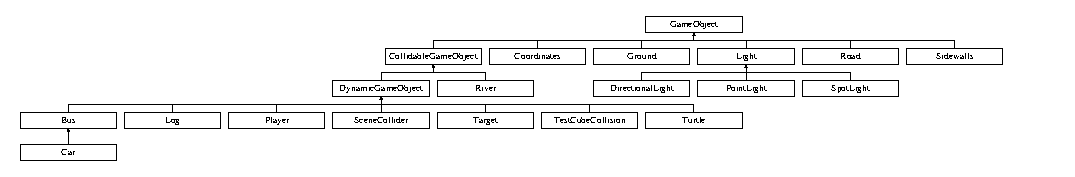
\includegraphics[height=1.931034cm]{class_game_object}
\end{center}
\end{figure}
\subsection*{Public Member Functions}
\begin{DoxyCompactItemize}
\item 
\hyperlink{class_game_object_ac95c474744d79fe4aadc49a100cfb9c6}{Game\+Object} (\hyperlink{class_vector3}{Vector3} pos)
\item 
void \hyperlink{class_game_object_a218c4b2970c9385f524b4cf5a13a3883}{set\+Enabled} (bool state)
\item 
bool \hyperlink{class_game_object_afd4da74521b2ba311f82b62f6ffec9e3}{is\+Enabled} ()
\item 
bool \hyperlink{class_game_object_ae3a7ab65df0dc3fb241a5a35a390fb3b}{get\+Animation\+Enabled} ()
\item 
void \hyperlink{class_game_object_a75027d1b9e11cd22111535b29ff062e0}{set\+Animation\+Enabled} (bool new\+Animation\+Enabled\+State)
\item 
virtual void \hyperlink{class_game_object_aecb2c1b9f69715d854f7604d5d7978ec}{init} ()
\item 
virtual void \hyperlink{class_game_object_a484efb66a7a27c101e84c11d9905d7a6}{render} ()
\item 
virtual void \hyperlink{class_game_object_a6dc5215a3d0efc7a9e2332006b31c868}{update} (int \hyperlink{_game_manager_8h_afea6a95c7a1c119b7106a4c735eb259d}{delta\+Time})
\item 
virtual \hyperlink{_game_object_8h_a57678b60d65afb213d04a6b090c64a08}{Game\+Object\+Type} \hyperlink{class_game_object_ab7ee421293a4bbe47b4102180185fbaa}{get\+Type} ()
\item 
virtual \hyperlink{class_vector3}{Vector3} \hyperlink{class_game_object_ac08043ba5563ecbd118e522169f7f919}{get\+Speed} ()
\item 
virtual bool \hyperlink{class_game_object_a9ab7d2e2beff3e91ccdc87c9fbca019e}{collide\+With} (const \hyperlink{class_game_object}{Game\+Object} $\ast$other) const
\item 
virtual \hyperlink{class_bounding_box}{Bounding\+Box} \hyperlink{class_game_object_a64b37bea01266aea52a47f4a48a9cc84}{get\+Bounding\+Box} () const
\item 
virtual float \hyperlink{class_game_object_a577ca32504b1551f75e1724219c4f6cf}{get\+Speed\+Multiplier} () const
\item 
virtual void \hyperlink{class_game_object_ab3d0617433250c19ccbb64bfca1bb905}{set\+Speed\+Multiplier} (float new\+Speed\+Mult)
\end{DoxyCompactItemize}
\subsection*{Public Attributes}
\begin{DoxyCompactItemize}
\item 
\hyperlink{class_vector3}{Vector3} \hyperlink{class_game_object_abdc7864253235aced4171f9a6eeae6e1}{position}
\end{DoxyCompactItemize}
\subsection*{Static Protected Member Functions}
\begin{DoxyCompactItemize}
\item 
static void \hyperlink{class_game_object_a7607cef4104343b5b6b91c40f8045fbd}{render\+Materials} (G\+Lint mid)
\item 
static void \hyperlink{class_game_object_aac4766680e60cb120df6636e57c4d269}{render\+Texture} (G\+Lint mid)
\item 
static void \hyperlink{class_game_object_a9cf3bf44182a7b73c714e64981e3c510}{set\+Material} (G\+Lint mid, \hyperlink{struct_a_material}{A\+Material} mat)
\item 
static \hyperlink{struct_shader_indices}{Shader\+Indices} \hyperlink{class_game_object_a8fac812880b4c8c086b9263ffb2e88b3}{get\+Pointers} (G\+Lint mid)
\item 
static void \hyperlink{class_game_object_a9fc6cfc23e66aeb60bc6d3eb8ac0c351}{build\+V\+AO} (G\+Lint mid)
\end{DoxyCompactItemize}
\subsection*{Protected Attributes}
\begin{DoxyCompactItemize}
\item 
bool \hyperlink{class_game_object_a1ddc5fba8005a5269bfb282022f6f736}{enabled} = true
\item 
bool \hyperlink{class_game_object_a83e4944f434a732494fd3410ab2a0123}{animation\+Enabled} = true
\item 
std\+::vector$<$ int $>$ \hyperlink{class_game_object_a2213b69db0d43fe8b6a7badb176950f8}{ids} = \{\}
\end{DoxyCompactItemize}
\subsection*{Static Protected Attributes}
\begin{DoxyCompactItemize}
\item 
static int \hyperlink{class_game_object_a3410079d3cfee94a22b5d6a885991165}{id\+Count} = 0
\end{DoxyCompactItemize}


\subsection{Constructor \& Destructor Documentation}
\mbox{\Hypertarget{class_game_object_ac95c474744d79fe4aadc49a100cfb9c6}\label{class_game_object_ac95c474744d79fe4aadc49a100cfb9c6}} 
\index{Game\+Object@{Game\+Object}!Game\+Object@{Game\+Object}}
\index{Game\+Object@{Game\+Object}!Game\+Object@{Game\+Object}}
\subsubsection{\texorpdfstring{Game\+Object()}{GameObject()}}
{\footnotesize\ttfamily Game\+Object\+::\+Game\+Object (\begin{DoxyParamCaption}\item[{\hyperlink{class_vector3}{Vector3}}]{pos }\end{DoxyParamCaption})\hspace{0.3cm}{\ttfamily [inline]}}



\subsection{Member Function Documentation}
\mbox{\Hypertarget{class_game_object_a9fc6cfc23e66aeb60bc6d3eb8ac0c351}\label{class_game_object_a9fc6cfc23e66aeb60bc6d3eb8ac0c351}} 
\index{Game\+Object@{Game\+Object}!build\+V\+AO@{build\+V\+AO}}
\index{build\+V\+AO@{build\+V\+AO}!Game\+Object@{Game\+Object}}
\subsubsection{\texorpdfstring{build\+V\+A\+O()}{buildVAO()}}
{\footnotesize\ttfamily static void Game\+Object\+::build\+V\+AO (\begin{DoxyParamCaption}\item[{G\+Lint}]{mid }\end{DoxyParamCaption})\hspace{0.3cm}{\ttfamily [inline]}, {\ttfamily [static]}, {\ttfamily [protected]}}

\mbox{\Hypertarget{class_game_object_a9ab7d2e2beff3e91ccdc87c9fbca019e}\label{class_game_object_a9ab7d2e2beff3e91ccdc87c9fbca019e}} 
\index{Game\+Object@{Game\+Object}!collide\+With@{collide\+With}}
\index{collide\+With@{collide\+With}!Game\+Object@{Game\+Object}}
\subsubsection{\texorpdfstring{collide\+With()}{collideWith()}}
{\footnotesize\ttfamily virtual bool Game\+Object\+::collide\+With (\begin{DoxyParamCaption}\item[{const \hyperlink{class_game_object}{Game\+Object} $\ast$}]{other }\end{DoxyParamCaption}) const\hspace{0.3cm}{\ttfamily [inline]}, {\ttfamily [virtual]}}



Reimplemented in \hyperlink{class_collidable_game_object_aabc837db5ee83847ad55a5f95cb106a6}{Collidable\+Game\+Object}.

\mbox{\Hypertarget{class_game_object_ae3a7ab65df0dc3fb241a5a35a390fb3b}\label{class_game_object_ae3a7ab65df0dc3fb241a5a35a390fb3b}} 
\index{Game\+Object@{Game\+Object}!get\+Animation\+Enabled@{get\+Animation\+Enabled}}
\index{get\+Animation\+Enabled@{get\+Animation\+Enabled}!Game\+Object@{Game\+Object}}
\subsubsection{\texorpdfstring{get\+Animation\+Enabled()}{getAnimationEnabled()}}
{\footnotesize\ttfamily bool Game\+Object\+::get\+Animation\+Enabled (\begin{DoxyParamCaption}{ }\end{DoxyParamCaption})\hspace{0.3cm}{\ttfamily [inline]}}

\mbox{\Hypertarget{class_game_object_a64b37bea01266aea52a47f4a48a9cc84}\label{class_game_object_a64b37bea01266aea52a47f4a48a9cc84}} 
\index{Game\+Object@{Game\+Object}!get\+Bounding\+Box@{get\+Bounding\+Box}}
\index{get\+Bounding\+Box@{get\+Bounding\+Box}!Game\+Object@{Game\+Object}}
\subsubsection{\texorpdfstring{get\+Bounding\+Box()}{getBoundingBox()}}
{\footnotesize\ttfamily virtual \hyperlink{class_bounding_box}{Bounding\+Box} Game\+Object\+::get\+Bounding\+Box (\begin{DoxyParamCaption}{ }\end{DoxyParamCaption}) const\hspace{0.3cm}{\ttfamily [inline]}, {\ttfamily [virtual]}}



Reimplemented in \hyperlink{class_collidable_game_object_a7998e4aabd23263212e72f6a40d42036}{Collidable\+Game\+Object}.

\mbox{\Hypertarget{class_game_object_a8fac812880b4c8c086b9263ffb2e88b3}\label{class_game_object_a8fac812880b4c8c086b9263ffb2e88b3}} 
\index{Game\+Object@{Game\+Object}!get\+Pointers@{get\+Pointers}}
\index{get\+Pointers@{get\+Pointers}!Game\+Object@{Game\+Object}}
\subsubsection{\texorpdfstring{get\+Pointers()}{getPointers()}}
{\footnotesize\ttfamily static \hyperlink{struct_shader_indices}{Shader\+Indices} Game\+Object\+::get\+Pointers (\begin{DoxyParamCaption}\item[{G\+Lint}]{mid }\end{DoxyParamCaption})\hspace{0.3cm}{\ttfamily [inline]}, {\ttfamily [static]}, {\ttfamily [protected]}}

\mbox{\Hypertarget{class_game_object_ac08043ba5563ecbd118e522169f7f919}\label{class_game_object_ac08043ba5563ecbd118e522169f7f919}} 
\index{Game\+Object@{Game\+Object}!get\+Speed@{get\+Speed}}
\index{get\+Speed@{get\+Speed}!Game\+Object@{Game\+Object}}
\subsubsection{\texorpdfstring{get\+Speed()}{getSpeed()}}
{\footnotesize\ttfamily virtual \hyperlink{class_vector3}{Vector3} Game\+Object\+::get\+Speed (\begin{DoxyParamCaption}{ }\end{DoxyParamCaption})\hspace{0.3cm}{\ttfamily [inline]}, {\ttfamily [virtual]}}



Reimplemented in \hyperlink{class_dynamic_game_object_a22d2cededc50901db950ac23b46e4d42}{Dynamic\+Game\+Object}.

\mbox{\Hypertarget{class_game_object_a577ca32504b1551f75e1724219c4f6cf}\label{class_game_object_a577ca32504b1551f75e1724219c4f6cf}} 
\index{Game\+Object@{Game\+Object}!get\+Speed\+Multiplier@{get\+Speed\+Multiplier}}
\index{get\+Speed\+Multiplier@{get\+Speed\+Multiplier}!Game\+Object@{Game\+Object}}
\subsubsection{\texorpdfstring{get\+Speed\+Multiplier()}{getSpeedMultiplier()}}
{\footnotesize\ttfamily virtual float Game\+Object\+::get\+Speed\+Multiplier (\begin{DoxyParamCaption}{ }\end{DoxyParamCaption}) const\hspace{0.3cm}{\ttfamily [inline]}, {\ttfamily [virtual]}}



Reimplemented in \hyperlink{class_dynamic_game_object_a677f4bdcd11800fee831a13234382619}{Dynamic\+Game\+Object}.

\mbox{\Hypertarget{class_game_object_ab7ee421293a4bbe47b4102180185fbaa}\label{class_game_object_ab7ee421293a4bbe47b4102180185fbaa}} 
\index{Game\+Object@{Game\+Object}!get\+Type@{get\+Type}}
\index{get\+Type@{get\+Type}!Game\+Object@{Game\+Object}}
\subsubsection{\texorpdfstring{get\+Type()}{getType()}}
{\footnotesize\ttfamily virtual \hyperlink{_game_object_8h_a57678b60d65afb213d04a6b090c64a08}{Game\+Object\+Type} Game\+Object\+::get\+Type (\begin{DoxyParamCaption}{ }\end{DoxyParamCaption})\hspace{0.3cm}{\ttfamily [inline]}, {\ttfamily [virtual]}}



Reimplemented in \hyperlink{class_collidable_game_object_a9890003d579d6318a4da31a0d540ab2f}{Collidable\+Game\+Object}.

\mbox{\Hypertarget{class_game_object_aecb2c1b9f69715d854f7604d5d7978ec}\label{class_game_object_aecb2c1b9f69715d854f7604d5d7978ec}} 
\index{Game\+Object@{Game\+Object}!init@{init}}
\index{init@{init}!Game\+Object@{Game\+Object}}
\subsubsection{\texorpdfstring{init()}{init()}}
{\footnotesize\ttfamily virtual void Game\+Object\+::init (\begin{DoxyParamCaption}{ }\end{DoxyParamCaption})\hspace{0.3cm}{\ttfamily [inline]}, {\ttfamily [virtual]}}



Reimplemented in \hyperlink{class_player_a1fb512423a77eee4ed0dea7cb7179c83}{Player}, \hyperlink{class_turtle_a6ba4b31af71ea52e0e885a3e3beb783c}{Turtle}, \hyperlink{class_log_aa6d8efc1a2ca7c84945bd129fe92448f}{Log}, \hyperlink{class_bus_a7bff316b767441b92f8e82f17a44fbf7}{Bus}, \hyperlink{class_test_cube_collision_a22fade1ca48a2cd49dd4ca6cbc93821b}{Test\+Cube\+Collision}, \hyperlink{class_road_a2d72b47fce205751e504929e91a7e567}{Road}, \hyperlink{class_target_aca691803b6bb7185adc521d63cdd7835}{Target}, \hyperlink{class_car_ae7d4da15bf41cc2d36465129372f2a71}{Car}, \hyperlink{class_sidewalls_a4d6161bfb13fe2779a9510c424879707}{Sidewalls}, \hyperlink{class_river_a34d39d986e411f957e77e85ba5719af4}{River}, \hyperlink{class_scene_collider_a2b2aae1d24b6f40188150d3002e00218}{Scene\+Collider}, \hyperlink{class_coordinates_aaadf934b8f184a9e0abe504e4c2da9b1}{Coordinates}, and \hyperlink{class_ground_a4680c2a6ab91627a71939a5a942409ac}{Ground}.

\mbox{\Hypertarget{class_game_object_afd4da74521b2ba311f82b62f6ffec9e3}\label{class_game_object_afd4da74521b2ba311f82b62f6ffec9e3}} 
\index{Game\+Object@{Game\+Object}!is\+Enabled@{is\+Enabled}}
\index{is\+Enabled@{is\+Enabled}!Game\+Object@{Game\+Object}}
\subsubsection{\texorpdfstring{is\+Enabled()}{isEnabled()}}
{\footnotesize\ttfamily bool Game\+Object\+::is\+Enabled (\begin{DoxyParamCaption}{ }\end{DoxyParamCaption})\hspace{0.3cm}{\ttfamily [inline]}}

\mbox{\Hypertarget{class_game_object_a484efb66a7a27c101e84c11d9905d7a6}\label{class_game_object_a484efb66a7a27c101e84c11d9905d7a6}} 
\index{Game\+Object@{Game\+Object}!render@{render}}
\index{render@{render}!Game\+Object@{Game\+Object}}
\subsubsection{\texorpdfstring{render()}{render()}}
{\footnotesize\ttfamily virtual void Game\+Object\+::render (\begin{DoxyParamCaption}{ }\end{DoxyParamCaption})\hspace{0.3cm}{\ttfamily [inline]}, {\ttfamily [virtual]}}



Reimplemented in \hyperlink{class_player_a4da76233f59ad0254aa6ec533f9badcc}{Player}, \hyperlink{class_bus_a0fe709af4b2ca86583d8647f323c231c}{Bus}, \hyperlink{class_turtle_a697924198490c52307fdb006f1df7456}{Turtle}, \hyperlink{class_car_a52c7156c403d267444de3d4813fffba2}{Car}, \hyperlink{class_log_a150966688120bfd2e4f29f57bbb65031}{Log}, \hyperlink{class_sidewalls_a3459ee5dee7a73043955607c5cb51d73}{Sidewalls}, \hyperlink{class_test_cube_collision_ae5cd1052745d6acf9cbb2a6bde8b757a}{Test\+Cube\+Collision}, \hyperlink{class_target_a03e4fae56bd104dadf5cec8247452c7e}{Target}, \hyperlink{class_coordinates_afa2d40b313b3b2933f9030ebfbe31045}{Coordinates}, \hyperlink{class_ground_a558a7774ca17a4fb4455a0e0d9f66a94}{Ground}, \hyperlink{class_road_a2ca4cc3c6043f6d1044992073e9fe3ba}{Road}, \hyperlink{class_river_abf5ba1cc4356fbf57059da23e3a1997a}{River}, \hyperlink{class_scene_collider_aa46bbfb6657449115aa6855a8f46e3f5}{Scene\+Collider}, \hyperlink{class_spot_light_a05dc942328210344caff20ffd58d0eb6}{Spot\+Light}, \hyperlink{class_directional_light_aa56c9af208dd1bc66967d219297b6e67}{Directional\+Light}, and \hyperlink{class_point_light_a4584cb5e40e5dd6ab2f43ec84851152c}{Point\+Light}.

\mbox{\Hypertarget{class_game_object_a7607cef4104343b5b6b91c40f8045fbd}\label{class_game_object_a7607cef4104343b5b6b91c40f8045fbd}} 
\index{Game\+Object@{Game\+Object}!render\+Materials@{render\+Materials}}
\index{render\+Materials@{render\+Materials}!Game\+Object@{Game\+Object}}
\subsubsection{\texorpdfstring{render\+Materials()}{renderMaterials()}}
{\footnotesize\ttfamily static void Game\+Object\+::render\+Materials (\begin{DoxyParamCaption}\item[{G\+Lint}]{mid }\end{DoxyParamCaption})\hspace{0.3cm}{\ttfamily [inline]}, {\ttfamily [static]}, {\ttfamily [protected]}}

\mbox{\Hypertarget{class_game_object_aac4766680e60cb120df6636e57c4d269}\label{class_game_object_aac4766680e60cb120df6636e57c4d269}} 
\index{Game\+Object@{Game\+Object}!render\+Texture@{render\+Texture}}
\index{render\+Texture@{render\+Texture}!Game\+Object@{Game\+Object}}
\subsubsection{\texorpdfstring{render\+Texture()}{renderTexture()}}
{\footnotesize\ttfamily static void Game\+Object\+::render\+Texture (\begin{DoxyParamCaption}\item[{G\+Lint}]{mid }\end{DoxyParamCaption})\hspace{0.3cm}{\ttfamily [inline]}, {\ttfamily [static]}, {\ttfamily [protected]}}

\mbox{\Hypertarget{class_game_object_a75027d1b9e11cd22111535b29ff062e0}\label{class_game_object_a75027d1b9e11cd22111535b29ff062e0}} 
\index{Game\+Object@{Game\+Object}!set\+Animation\+Enabled@{set\+Animation\+Enabled}}
\index{set\+Animation\+Enabled@{set\+Animation\+Enabled}!Game\+Object@{Game\+Object}}
\subsubsection{\texorpdfstring{set\+Animation\+Enabled()}{setAnimationEnabled()}}
{\footnotesize\ttfamily void Game\+Object\+::set\+Animation\+Enabled (\begin{DoxyParamCaption}\item[{bool}]{new\+Animation\+Enabled\+State }\end{DoxyParamCaption})\hspace{0.3cm}{\ttfamily [inline]}}

\mbox{\Hypertarget{class_game_object_a218c4b2970c9385f524b4cf5a13a3883}\label{class_game_object_a218c4b2970c9385f524b4cf5a13a3883}} 
\index{Game\+Object@{Game\+Object}!set\+Enabled@{set\+Enabled}}
\index{set\+Enabled@{set\+Enabled}!Game\+Object@{Game\+Object}}
\subsubsection{\texorpdfstring{set\+Enabled()}{setEnabled()}}
{\footnotesize\ttfamily void Game\+Object\+::set\+Enabled (\begin{DoxyParamCaption}\item[{bool}]{state }\end{DoxyParamCaption})\hspace{0.3cm}{\ttfamily [inline]}}

\mbox{\Hypertarget{class_game_object_a9cf3bf44182a7b73c714e64981e3c510}\label{class_game_object_a9cf3bf44182a7b73c714e64981e3c510}} 
\index{Game\+Object@{Game\+Object}!set\+Material@{set\+Material}}
\index{set\+Material@{set\+Material}!Game\+Object@{Game\+Object}}
\subsubsection{\texorpdfstring{set\+Material()}{setMaterial()}}
{\footnotesize\ttfamily static void Game\+Object\+::set\+Material (\begin{DoxyParamCaption}\item[{G\+Lint}]{mid,  }\item[{\hyperlink{struct_a_material}{A\+Material}}]{mat }\end{DoxyParamCaption})\hspace{0.3cm}{\ttfamily [inline]}, {\ttfamily [static]}, {\ttfamily [protected]}}

\mbox{\Hypertarget{class_game_object_ab3d0617433250c19ccbb64bfca1bb905}\label{class_game_object_ab3d0617433250c19ccbb64bfca1bb905}} 
\index{Game\+Object@{Game\+Object}!set\+Speed\+Multiplier@{set\+Speed\+Multiplier}}
\index{set\+Speed\+Multiplier@{set\+Speed\+Multiplier}!Game\+Object@{Game\+Object}}
\subsubsection{\texorpdfstring{set\+Speed\+Multiplier()}{setSpeedMultiplier()}}
{\footnotesize\ttfamily virtual void Game\+Object\+::set\+Speed\+Multiplier (\begin{DoxyParamCaption}\item[{float}]{new\+Speed\+Mult }\end{DoxyParamCaption})\hspace{0.3cm}{\ttfamily [inline]}, {\ttfamily [virtual]}}



Reimplemented in \hyperlink{class_player_a9098e6b411ea9102b02bb911eca6515b}{Player}, and \hyperlink{class_dynamic_game_object_a7bf254357b0d2491044d175afdc36ca4}{Dynamic\+Game\+Object}.

\mbox{\Hypertarget{class_game_object_a6dc5215a3d0efc7a9e2332006b31c868}\label{class_game_object_a6dc5215a3d0efc7a9e2332006b31c868}} 
\index{Game\+Object@{Game\+Object}!update@{update}}
\index{update@{update}!Game\+Object@{Game\+Object}}
\subsubsection{\texorpdfstring{update()}{update()}}
{\footnotesize\ttfamily virtual void Game\+Object\+::update (\begin{DoxyParamCaption}\item[{int}]{delta\+Time }\end{DoxyParamCaption})\hspace{0.3cm}{\ttfamily [inline]}, {\ttfamily [virtual]}}



Reimplemented in \hyperlink{class_turtle_a6d62e3f4e21f5ce3ffb4e7e2a8a9da1b}{Turtle}, \hyperlink{class_player_a51e705a6ad3628144e02832d1839b360}{Player}, \hyperlink{class_bus_ad07157ce2a50211ea599d040da7a4517}{Bus}, \hyperlink{class_test_cube_collision_ae528ac632377372d93964c938748fddf}{Test\+Cube\+Collision}, \hyperlink{class_dynamic_game_object_aaa505b57d131bbbce44d500ec2ca0e83}{Dynamic\+Game\+Object}, and \hyperlink{class_target_a5f3b2dc70e8065e53199ab3244059ba7}{Target}.



\subsection{Member Data Documentation}
\mbox{\Hypertarget{class_game_object_a83e4944f434a732494fd3410ab2a0123}\label{class_game_object_a83e4944f434a732494fd3410ab2a0123}} 
\index{Game\+Object@{Game\+Object}!animation\+Enabled@{animation\+Enabled}}
\index{animation\+Enabled@{animation\+Enabled}!Game\+Object@{Game\+Object}}
\subsubsection{\texorpdfstring{animation\+Enabled}{animationEnabled}}
{\footnotesize\ttfamily bool Game\+Object\+::animation\+Enabled = true\hspace{0.3cm}{\ttfamily [protected]}}

\mbox{\Hypertarget{class_game_object_a1ddc5fba8005a5269bfb282022f6f736}\label{class_game_object_a1ddc5fba8005a5269bfb282022f6f736}} 
\index{Game\+Object@{Game\+Object}!enabled@{enabled}}
\index{enabled@{enabled}!Game\+Object@{Game\+Object}}
\subsubsection{\texorpdfstring{enabled}{enabled}}
{\footnotesize\ttfamily bool Game\+Object\+::enabled = true\hspace{0.3cm}{\ttfamily [protected]}}

\mbox{\Hypertarget{class_game_object_a3410079d3cfee94a22b5d6a885991165}\label{class_game_object_a3410079d3cfee94a22b5d6a885991165}} 
\index{Game\+Object@{Game\+Object}!id\+Count@{id\+Count}}
\index{id\+Count@{id\+Count}!Game\+Object@{Game\+Object}}
\subsubsection{\texorpdfstring{id\+Count}{idCount}}
{\footnotesize\ttfamily int Game\+Object\+::id\+Count = 0\hspace{0.3cm}{\ttfamily [static]}, {\ttfamily [protected]}}

\mbox{\Hypertarget{class_game_object_a2213b69db0d43fe8b6a7badb176950f8}\label{class_game_object_a2213b69db0d43fe8b6a7badb176950f8}} 
\index{Game\+Object@{Game\+Object}!ids@{ids}}
\index{ids@{ids}!Game\+Object@{Game\+Object}}
\subsubsection{\texorpdfstring{ids}{ids}}
{\footnotesize\ttfamily std\+::vector$<$int$>$ Game\+Object\+::ids = \{\}\hspace{0.3cm}{\ttfamily [protected]}}

\mbox{\Hypertarget{class_game_object_abdc7864253235aced4171f9a6eeae6e1}\label{class_game_object_abdc7864253235aced4171f9a6eeae6e1}} 
\index{Game\+Object@{Game\+Object}!position@{position}}
\index{position@{position}!Game\+Object@{Game\+Object}}
\subsubsection{\texorpdfstring{position}{position}}
{\footnotesize\ttfamily \hyperlink{class_vector3}{Vector3} Game\+Object\+::position}



The documentation for this class was generated from the following file\+:\begin{DoxyCompactItemize}
\item 
/\+Users/matya/\+A\+V\+T7/src/\hyperlink{_game_object_8h}{Game\+Object.\+h}\end{DoxyCompactItemize}

\hypertarget{class_ground}{}\section{Ground Class Reference}
\label{class_ground}\index{Ground@{Ground}}


{\ttfamily \#include $<$Ground.\+h$>$}

Inheritance diagram for Ground\+:\begin{figure}[H]
\begin{center}
\leavevmode
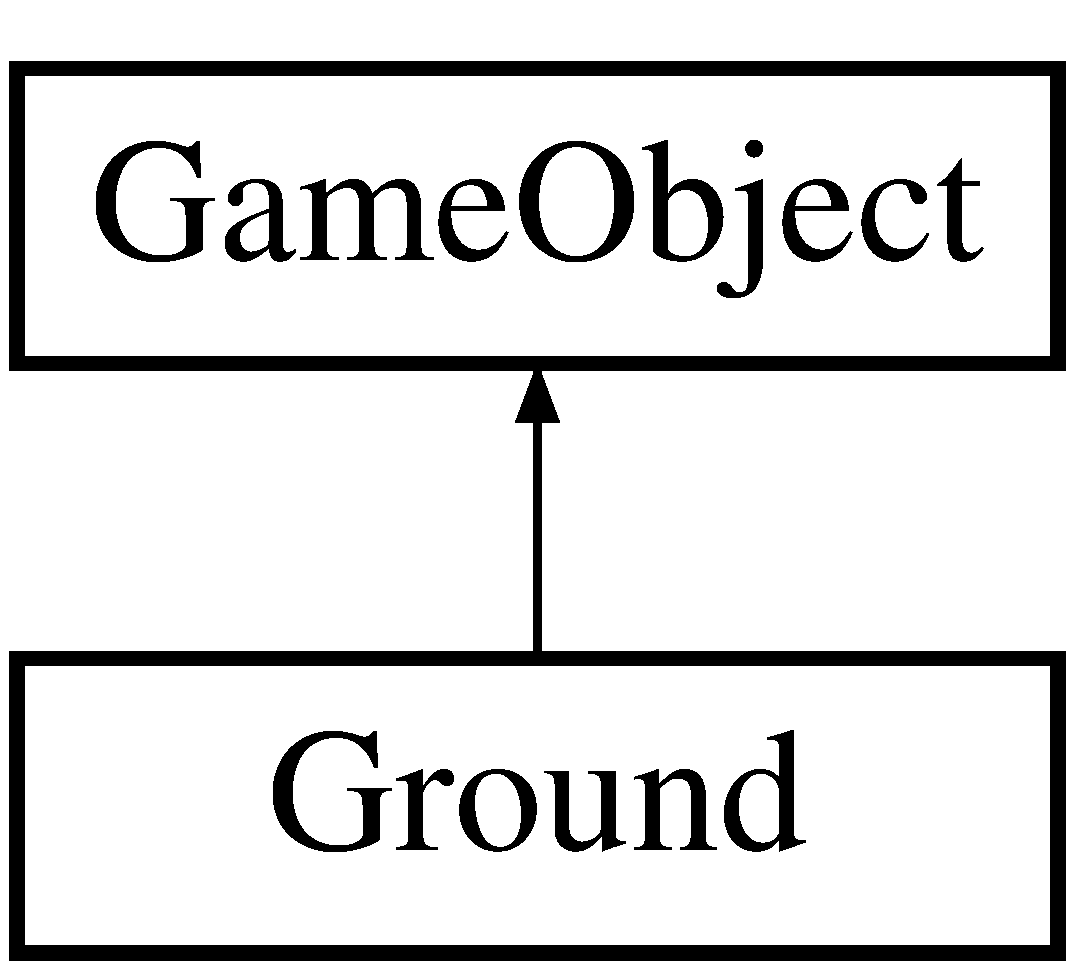
\includegraphics[height=2.000000cm]{class_ground}
\end{center}
\end{figure}
\subsection*{Public Member Functions}
\begin{DoxyCompactItemize}
\item 
\hyperlink{class_ground_abe733811bf44d4791c7811a5f71aae25}{Ground} ()
\item 
void \hyperlink{class_ground_a4680c2a6ab91627a71939a5a942409ac}{init} () override
\item 
void \hyperlink{class_ground_a558a7774ca17a4fb4455a0e0d9f66a94}{render} () override
\end{DoxyCompactItemize}
\subsection*{Additional Inherited Members}


\subsection{Constructor \& Destructor Documentation}
\mbox{\Hypertarget{class_ground_abe733811bf44d4791c7811a5f71aae25}\label{class_ground_abe733811bf44d4791c7811a5f71aae25}} 
\index{Ground@{Ground}!Ground@{Ground}}
\index{Ground@{Ground}!Ground@{Ground}}
\subsubsection{\texorpdfstring{Ground()}{Ground()}}
{\footnotesize\ttfamily Ground\+::\+Ground (\begin{DoxyParamCaption}{ }\end{DoxyParamCaption})\hspace{0.3cm}{\ttfamily [inline]}, {\ttfamily [explicit]}}



\subsection{Member Function Documentation}
\mbox{\Hypertarget{class_ground_a4680c2a6ab91627a71939a5a942409ac}\label{class_ground_a4680c2a6ab91627a71939a5a942409ac}} 
\index{Ground@{Ground}!init@{init}}
\index{init@{init}!Ground@{Ground}}
\subsubsection{\texorpdfstring{init()}{init()}}
{\footnotesize\ttfamily void Ground\+::init (\begin{DoxyParamCaption}{ }\end{DoxyParamCaption})\hspace{0.3cm}{\ttfamily [inline]}, {\ttfamily [override]}, {\ttfamily [virtual]}}



Reimplemented from \hyperlink{class_game_object_aecb2c1b9f69715d854f7604d5d7978ec}{Game\+Object}.

\mbox{\Hypertarget{class_ground_a558a7774ca17a4fb4455a0e0d9f66a94}\label{class_ground_a558a7774ca17a4fb4455a0e0d9f66a94}} 
\index{Ground@{Ground}!render@{render}}
\index{render@{render}!Ground@{Ground}}
\subsubsection{\texorpdfstring{render()}{render()}}
{\footnotesize\ttfamily void Ground\+::render (\begin{DoxyParamCaption}{ }\end{DoxyParamCaption})\hspace{0.3cm}{\ttfamily [inline]}, {\ttfamily [override]}, {\ttfamily [virtual]}}



Reimplemented from \hyperlink{class_game_object_a484efb66a7a27c101e84c11d9905d7a6}{Game\+Object}.



The documentation for this class was generated from the following file\+:\begin{DoxyCompactItemize}
\item 
/\+Users/matya/\+A\+V\+T7/src/objects/\hyperlink{_ground_8h}{Ground.\+h}\end{DoxyCompactItemize}

\hypertarget{class_light}{}\section{Light Class Reference}
\label{class_light}\index{Light@{Light}}


{\ttfamily \#include $<$Light.\+h$>$}

Inheritance diagram for Light\+:\begin{figure}[H]
\begin{center}
\leavevmode
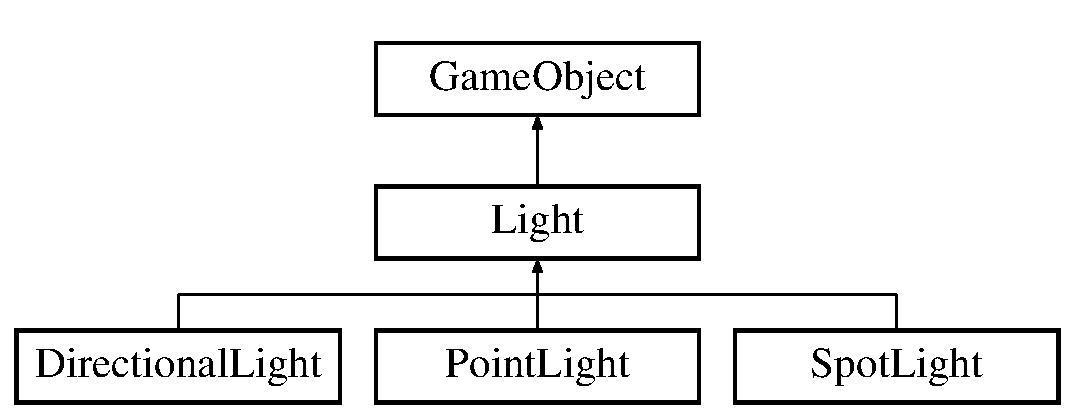
\includegraphics[height=3.000000cm]{class_light}
\end{center}
\end{figure}
\subsection*{Public Member Functions}
\begin{DoxyCompactItemize}
\item 
void \hyperlink{class_light_ae0b3607b306357b4b4540e8759ef3fbf}{toggle\+Light} ()
\end{DoxyCompactItemize}
\subsection*{Protected Member Functions}
\begin{DoxyCompactItemize}
\item 
\hyperlink{class_light_a87c35098e794c0b8c929308145e0786e}{Light} (\hyperlink{class_vector3}{Vector3} pos, int \hyperlink{class_light_ae0028340ad3a9f2e196b68365d5fe972}{light\+\_\+id}, bool light\+\_\+active=true)
\item 
void \hyperlink{class_light_a0fbb865c0d4810c4521ecc92dfd69a0f}{set\+Light\+Enabled} (bool new\+State)
\end{DoxyCompactItemize}
\subsection*{Protected Attributes}
\begin{DoxyCompactItemize}
\item 
bool \hyperlink{class_light_ab622899f496ea310685e6cbb45977cac}{light\+\_\+enabled}
\item 
int \hyperlink{class_light_ae0028340ad3a9f2e196b68365d5fe972}{light\+\_\+id}
\end{DoxyCompactItemize}
\subsection*{Additional Inherited Members}


\subsection{Constructor \& Destructor Documentation}
\mbox{\Hypertarget{class_light_a87c35098e794c0b8c929308145e0786e}\label{class_light_a87c35098e794c0b8c929308145e0786e}} 
\index{Light@{Light}!Light@{Light}}
\index{Light@{Light}!Light@{Light}}
\subsubsection{\texorpdfstring{Light()}{Light()}}
{\footnotesize\ttfamily Light\+::\+Light (\begin{DoxyParamCaption}\item[{\hyperlink{class_vector3}{Vector3}}]{pos,  }\item[{int}]{light\+\_\+id,  }\item[{bool}]{light\+\_\+active = {\ttfamily true} }\end{DoxyParamCaption})\hspace{0.3cm}{\ttfamily [inline]}, {\ttfamily [explicit]}, {\ttfamily [protected]}}



\subsection{Member Function Documentation}
\mbox{\Hypertarget{class_light_a0fbb865c0d4810c4521ecc92dfd69a0f}\label{class_light_a0fbb865c0d4810c4521ecc92dfd69a0f}} 
\index{Light@{Light}!set\+Light\+Enabled@{set\+Light\+Enabled}}
\index{set\+Light\+Enabled@{set\+Light\+Enabled}!Light@{Light}}
\subsubsection{\texorpdfstring{set\+Light\+Enabled()}{setLightEnabled()}}
{\footnotesize\ttfamily void Light\+::set\+Light\+Enabled (\begin{DoxyParamCaption}\item[{bool}]{new\+State }\end{DoxyParamCaption})\hspace{0.3cm}{\ttfamily [inline]}, {\ttfamily [protected]}}

\mbox{\Hypertarget{class_light_ae0b3607b306357b4b4540e8759ef3fbf}\label{class_light_ae0b3607b306357b4b4540e8759ef3fbf}} 
\index{Light@{Light}!toggle\+Light@{toggle\+Light}}
\index{toggle\+Light@{toggle\+Light}!Light@{Light}}
\subsubsection{\texorpdfstring{toggle\+Light()}{toggleLight()}}
{\footnotesize\ttfamily void Light\+::toggle\+Light (\begin{DoxyParamCaption}{ }\end{DoxyParamCaption})\hspace{0.3cm}{\ttfamily [inline]}}



\subsection{Member Data Documentation}
\mbox{\Hypertarget{class_light_ab622899f496ea310685e6cbb45977cac}\label{class_light_ab622899f496ea310685e6cbb45977cac}} 
\index{Light@{Light}!light\+\_\+enabled@{light\+\_\+enabled}}
\index{light\+\_\+enabled@{light\+\_\+enabled}!Light@{Light}}
\subsubsection{\texorpdfstring{light\+\_\+enabled}{light\_enabled}}
{\footnotesize\ttfamily bool Light\+::light\+\_\+enabled\hspace{0.3cm}{\ttfamily [protected]}}

\mbox{\Hypertarget{class_light_ae0028340ad3a9f2e196b68365d5fe972}\label{class_light_ae0028340ad3a9f2e196b68365d5fe972}} 
\index{Light@{Light}!light\+\_\+id@{light\+\_\+id}}
\index{light\+\_\+id@{light\+\_\+id}!Light@{Light}}
\subsubsection{\texorpdfstring{light\+\_\+id}{light\_id}}
{\footnotesize\ttfamily int Light\+::light\+\_\+id\hspace{0.3cm}{\ttfamily [protected]}}



The documentation for this class was generated from the following file\+:\begin{DoxyCompactItemize}
\item 
/\+Users/matya/\+A\+V\+T7/src/objects/\hyperlink{_light_8h}{Light.\+h}\end{DoxyCompactItemize}

\hypertarget{class_log}{}\section{Log Class Reference}
\label{class_log}\index{Log@{Log}}


{\ttfamily \#include $<$Log.\+h$>$}

Inheritance diagram for Log\+:\begin{figure}[H]
\begin{center}
\leavevmode
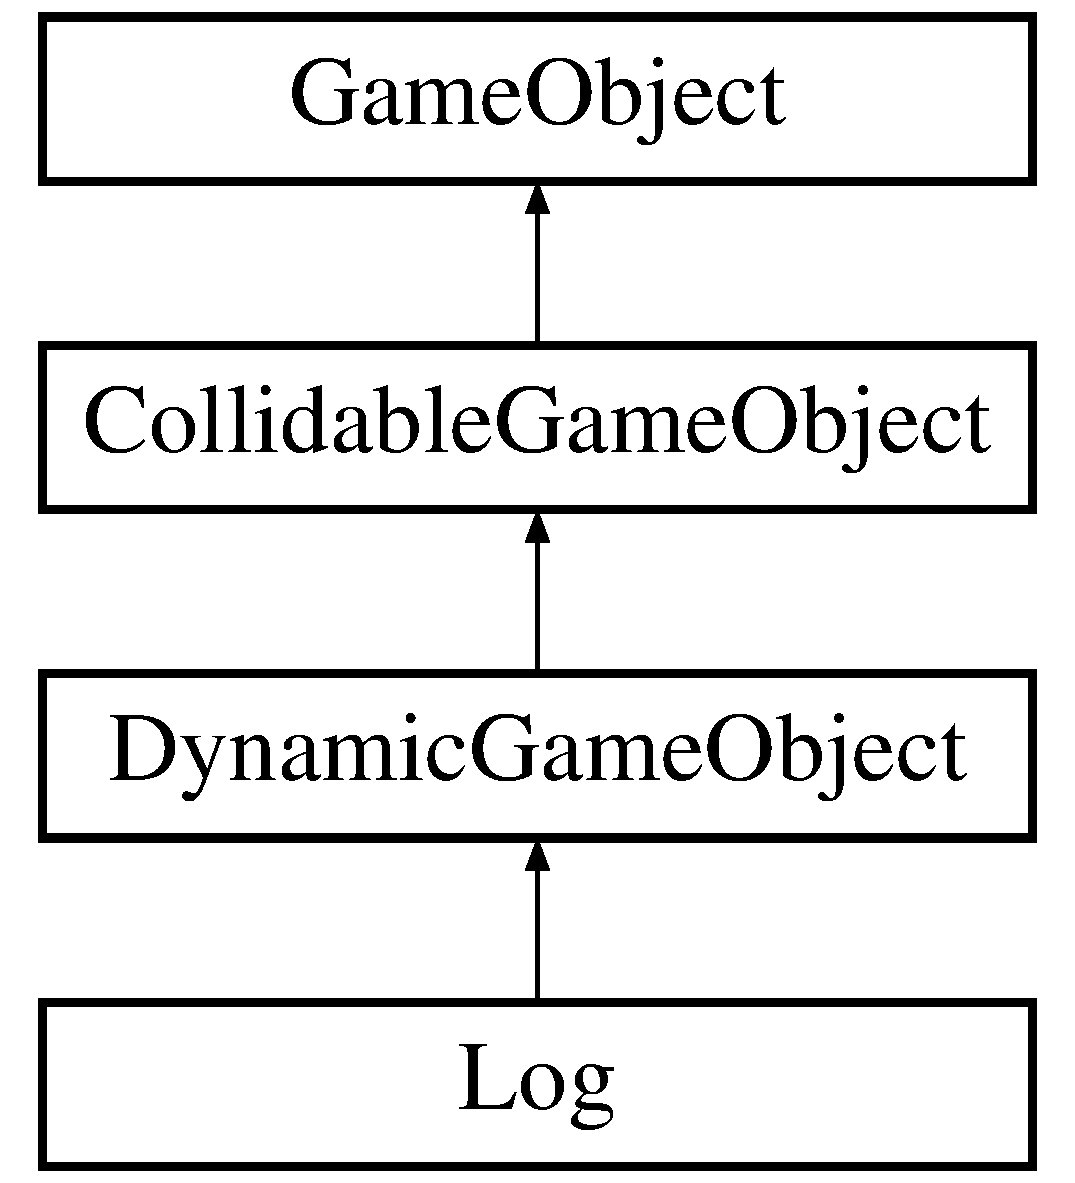
\includegraphics[height=4.000000cm]{class_log}
\end{center}
\end{figure}
\subsection*{Public Member Functions}
\begin{DoxyCompactItemize}
\item 
\hyperlink{class_log_aab0f1ee2fbfa2962846e0c84b032a11f}{Log} (\hyperlink{class_vector3}{Vector3} pos, \hyperlink{class_vector3}{Vector3} \hyperlink{class_dynamic_game_object_a54cb8a3a5fe8314cd5751f223b2b49ae}{speed})
\item 
void \hyperlink{class_log_aa6d8efc1a2ca7c84945bd129fe92448f}{init} () override
\item 
void \hyperlink{class_log_a150966688120bfd2e4f29f57bbb65031}{render} () override
\item 
void \hyperlink{class_log_a8f4f588a53320811a95a703fb1a9de8f}{respawn} ()
\item 
void \hyperlink{class_log_ae11177063e932d7895f09e826c685144}{rock\+Log} ()
\end{DoxyCompactItemize}
\subsection*{Public Attributes}
\begin{DoxyCompactItemize}
\item 
\hyperlink{class_vector3}{Vector3} \hyperlink{class_log_a0d213f7219bcc6ea0516da6041cd7911}{init\+Pos}
\item 
float \hyperlink{class_log_a427e736b62232ae99203aa37c20eedc0}{random\+Time\+Offset} = 0.\+0f
\item 
const float \hyperlink{class_log_a95b70921e749674648a01f04834e67df}{wave\+Time} = 500.\+0f
\item 
float \hyperlink{class_log_ab0b1ce09d317ec6ec5f16c9648cc196b}{angle} = 0
\item 
G\+Lint \hyperlink{class_log_a41c7e99b613a8c1d0fb664df5d21e01a}{delta\+Time} = 1
\item 
G\+Lint \hyperlink{class_log_ae1e50d0638372cc9976cc9de946a779b}{prev\+Time} = 1
\item 
\hyperlink{class_vector3}{Vector3} \hyperlink{class_log_a9eac71cb8f2c6006211c30493b235aa4}{init\+Speed}
\end{DoxyCompactItemize}
\subsection*{Additional Inherited Members}


\subsection{Constructor \& Destructor Documentation}
\mbox{\Hypertarget{class_log_aab0f1ee2fbfa2962846e0c84b032a11f}\label{class_log_aab0f1ee2fbfa2962846e0c84b032a11f}} 
\index{Log@{Log}!Log@{Log}}
\index{Log@{Log}!Log@{Log}}
\subsubsection{\texorpdfstring{Log()}{Log()}}
{\footnotesize\ttfamily Log\+::\+Log (\begin{DoxyParamCaption}\item[{\hyperlink{class_vector3}{Vector3}}]{pos,  }\item[{\hyperlink{class_vector3}{Vector3}}]{speed }\end{DoxyParamCaption})\hspace{0.3cm}{\ttfamily [inline]}}



\subsection{Member Function Documentation}
\mbox{\Hypertarget{class_log_aa6d8efc1a2ca7c84945bd129fe92448f}\label{class_log_aa6d8efc1a2ca7c84945bd129fe92448f}} 
\index{Log@{Log}!init@{init}}
\index{init@{init}!Log@{Log}}
\subsubsection{\texorpdfstring{init()}{init()}}
{\footnotesize\ttfamily void Log\+::init (\begin{DoxyParamCaption}{ }\end{DoxyParamCaption})\hspace{0.3cm}{\ttfamily [inline]}, {\ttfamily [override]}, {\ttfamily [virtual]}}



Reimplemented from \hyperlink{class_game_object_aecb2c1b9f69715d854f7604d5d7978ec}{Game\+Object}.

\mbox{\Hypertarget{class_log_a150966688120bfd2e4f29f57bbb65031}\label{class_log_a150966688120bfd2e4f29f57bbb65031}} 
\index{Log@{Log}!render@{render}}
\index{render@{render}!Log@{Log}}
\subsubsection{\texorpdfstring{render()}{render()}}
{\footnotesize\ttfamily void Log\+::render (\begin{DoxyParamCaption}{ }\end{DoxyParamCaption})\hspace{0.3cm}{\ttfamily [inline]}, {\ttfamily [override]}, {\ttfamily [virtual]}}



Reimplemented from \hyperlink{class_game_object_a484efb66a7a27c101e84c11d9905d7a6}{Game\+Object}.

\mbox{\Hypertarget{class_log_a8f4f588a53320811a95a703fb1a9de8f}\label{class_log_a8f4f588a53320811a95a703fb1a9de8f}} 
\index{Log@{Log}!respawn@{respawn}}
\index{respawn@{respawn}!Log@{Log}}
\subsubsection{\texorpdfstring{respawn()}{respawn()}}
{\footnotesize\ttfamily void Log\+::respawn (\begin{DoxyParamCaption}{ }\end{DoxyParamCaption})\hspace{0.3cm}{\ttfamily [inline]}}

\mbox{\Hypertarget{class_log_ae11177063e932d7895f09e826c685144}\label{class_log_ae11177063e932d7895f09e826c685144}} 
\index{Log@{Log}!rock\+Log@{rock\+Log}}
\index{rock\+Log@{rock\+Log}!Log@{Log}}
\subsubsection{\texorpdfstring{rock\+Log()}{rockLog()}}
{\footnotesize\ttfamily void Log\+::rock\+Log (\begin{DoxyParamCaption}{ }\end{DoxyParamCaption})\hspace{0.3cm}{\ttfamily [inline]}}



\subsection{Member Data Documentation}
\mbox{\Hypertarget{class_log_ab0b1ce09d317ec6ec5f16c9648cc196b}\label{class_log_ab0b1ce09d317ec6ec5f16c9648cc196b}} 
\index{Log@{Log}!angle@{angle}}
\index{angle@{angle}!Log@{Log}}
\subsubsection{\texorpdfstring{angle}{angle}}
{\footnotesize\ttfamily float Log\+::angle = 0}

\mbox{\Hypertarget{class_log_a41c7e99b613a8c1d0fb664df5d21e01a}\label{class_log_a41c7e99b613a8c1d0fb664df5d21e01a}} 
\index{Log@{Log}!delta\+Time@{delta\+Time}}
\index{delta\+Time@{delta\+Time}!Log@{Log}}
\subsubsection{\texorpdfstring{delta\+Time}{deltaTime}}
{\footnotesize\ttfamily G\+Lint Log\+::delta\+Time = 1}

\mbox{\Hypertarget{class_log_a0d213f7219bcc6ea0516da6041cd7911}\label{class_log_a0d213f7219bcc6ea0516da6041cd7911}} 
\index{Log@{Log}!init\+Pos@{init\+Pos}}
\index{init\+Pos@{init\+Pos}!Log@{Log}}
\subsubsection{\texorpdfstring{init\+Pos}{initPos}}
{\footnotesize\ttfamily \hyperlink{class_vector3}{Vector3} Log\+::init\+Pos}

\mbox{\Hypertarget{class_log_a9eac71cb8f2c6006211c30493b235aa4}\label{class_log_a9eac71cb8f2c6006211c30493b235aa4}} 
\index{Log@{Log}!init\+Speed@{init\+Speed}}
\index{init\+Speed@{init\+Speed}!Log@{Log}}
\subsubsection{\texorpdfstring{init\+Speed}{initSpeed}}
{\footnotesize\ttfamily \hyperlink{class_vector3}{Vector3} Log\+::init\+Speed}

\mbox{\Hypertarget{class_log_ae1e50d0638372cc9976cc9de946a779b}\label{class_log_ae1e50d0638372cc9976cc9de946a779b}} 
\index{Log@{Log}!prev\+Time@{prev\+Time}}
\index{prev\+Time@{prev\+Time}!Log@{Log}}
\subsubsection{\texorpdfstring{prev\+Time}{prevTime}}
{\footnotesize\ttfamily G\+Lint Log\+::prev\+Time = 1}

\mbox{\Hypertarget{class_log_a427e736b62232ae99203aa37c20eedc0}\label{class_log_a427e736b62232ae99203aa37c20eedc0}} 
\index{Log@{Log}!random\+Time\+Offset@{random\+Time\+Offset}}
\index{random\+Time\+Offset@{random\+Time\+Offset}!Log@{Log}}
\subsubsection{\texorpdfstring{random\+Time\+Offset}{randomTimeOffset}}
{\footnotesize\ttfamily float Log\+::random\+Time\+Offset = 0.\+0f}

\mbox{\Hypertarget{class_log_a95b70921e749674648a01f04834e67df}\label{class_log_a95b70921e749674648a01f04834e67df}} 
\index{Log@{Log}!wave\+Time@{wave\+Time}}
\index{wave\+Time@{wave\+Time}!Log@{Log}}
\subsubsection{\texorpdfstring{wave\+Time}{waveTime}}
{\footnotesize\ttfamily const float Log\+::wave\+Time = 500.\+0f}



The documentation for this class was generated from the following file\+:\begin{DoxyCompactItemize}
\item 
/\+Users/matya/\+A\+V\+T7/src/objects/\hyperlink{_log_8h}{Log.\+h}\end{DoxyCompactItemize}

\hypertarget{struct_material}{}\section{Material Struct Reference}
\label{struct_material}\index{Material@{Material}}


{\ttfamily \#include $<$basic\+\_\+geometry.\+h$>$}

\subsection*{Public Attributes}
\begin{DoxyCompactItemize}
\item 
float \hyperlink{struct_material_aa928d7b743a327e07cc5176e5d4d89c8}{diffuse} \mbox{[}4\mbox{]}
\item 
float \hyperlink{struct_material_a01a42e2eed3cd6662bd46786a441473a}{ambient} \mbox{[}4\mbox{]}
\item 
float \hyperlink{struct_material_a570719a080c2168e8c0225c085472c64}{specular} \mbox{[}4\mbox{]}
\item 
float \hyperlink{struct_material_a374ee687979c26f4a9e3d671d89a9751}{emissive} \mbox{[}4\mbox{]}
\item 
float \hyperlink{struct_material_a9dc184c883ec135ace28c1917af3fe84}{shininess}
\item 
int \hyperlink{struct_material_ad0964c5d437284a4dc9cfbe6e6dcafcc}{tex\+Count}
\end{DoxyCompactItemize}


\subsection{Member Data Documentation}
\mbox{\Hypertarget{struct_material_a01a42e2eed3cd6662bd46786a441473a}\label{struct_material_a01a42e2eed3cd6662bd46786a441473a}} 
\index{Material@{Material}!ambient@{ambient}}
\index{ambient@{ambient}!Material@{Material}}
\subsubsection{\texorpdfstring{ambient}{ambient}}
{\footnotesize\ttfamily float Material\+::ambient\mbox{[}4\mbox{]}}

\mbox{\Hypertarget{struct_material_aa928d7b743a327e07cc5176e5d4d89c8}\label{struct_material_aa928d7b743a327e07cc5176e5d4d89c8}} 
\index{Material@{Material}!diffuse@{diffuse}}
\index{diffuse@{diffuse}!Material@{Material}}
\subsubsection{\texorpdfstring{diffuse}{diffuse}}
{\footnotesize\ttfamily float Material\+::diffuse\mbox{[}4\mbox{]}}

\mbox{\Hypertarget{struct_material_a374ee687979c26f4a9e3d671d89a9751}\label{struct_material_a374ee687979c26f4a9e3d671d89a9751}} 
\index{Material@{Material}!emissive@{emissive}}
\index{emissive@{emissive}!Material@{Material}}
\subsubsection{\texorpdfstring{emissive}{emissive}}
{\footnotesize\ttfamily float Material\+::emissive\mbox{[}4\mbox{]}}

\mbox{\Hypertarget{struct_material_a9dc184c883ec135ace28c1917af3fe84}\label{struct_material_a9dc184c883ec135ace28c1917af3fe84}} 
\index{Material@{Material}!shininess@{shininess}}
\index{shininess@{shininess}!Material@{Material}}
\subsubsection{\texorpdfstring{shininess}{shininess}}
{\footnotesize\ttfamily float Material\+::shininess}

\mbox{\Hypertarget{struct_material_a570719a080c2168e8c0225c085472c64}\label{struct_material_a570719a080c2168e8c0225c085472c64}} 
\index{Material@{Material}!specular@{specular}}
\index{specular@{specular}!Material@{Material}}
\subsubsection{\texorpdfstring{specular}{specular}}
{\footnotesize\ttfamily float Material\+::specular\mbox{[}4\mbox{]}}

\mbox{\Hypertarget{struct_material_ad0964c5d437284a4dc9cfbe6e6dcafcc}\label{struct_material_ad0964c5d437284a4dc9cfbe6e6dcafcc}} 
\index{Material@{Material}!tex\+Count@{tex\+Count}}
\index{tex\+Count@{tex\+Count}!Material@{Material}}
\subsubsection{\texorpdfstring{tex\+Count}{texCount}}
{\footnotesize\ttfamily int Material\+::tex\+Count}



The documentation for this struct was generated from the following file\+:\begin{DoxyCompactItemize}
\item 
/\+Users/matya/\+A\+V\+T7/src/libs/\hyperlink{basic__geometry_8h}{basic\+\_\+geometry.\+h}\end{DoxyCompactItemize}

\hypertarget{struct_my_mesh}{}\section{My\+Mesh Struct Reference}
\label{struct_my_mesh}\index{My\+Mesh@{My\+Mesh}}


{\ttfamily \#include $<$basic\+\_\+geometry.\+h$>$}

\subsection*{Public Attributes}
\begin{DoxyCompactItemize}
\item 
G\+Luint \hyperlink{struct_my_mesh_a2e84e6ea2bf5ce3aa936e456577e7721}{vao}
\item 
G\+Luint \hyperlink{struct_my_mesh_a34f62cc69d253d529ede8a3c8f0c1530}{tex\+Units} \mbox{[}\hyperlink{basic__geometry_8h_ab5ca8e84cfd9b7c93955bc48faa7930c}{M\+A\+X\+I\+M\+U\+M\+\_\+\+T\+E\+X\+T\+U\+R\+ES}\mbox{]}
\item 
G\+Luint \hyperlink{struct_my_mesh_aabe1aa11c8b6419195d6f2ad1e0af294}{tex\+Types} \mbox{[}\hyperlink{basic__geometry_8h_ab5ca8e84cfd9b7c93955bc48faa7930c}{M\+A\+X\+I\+M\+U\+M\+\_\+\+T\+E\+X\+T\+U\+R\+ES}\mbox{]}
\item 
float \hyperlink{struct_my_mesh_aae0713b17789ccd6cbbf6b180186e3d9}{transform} \mbox{[}16\mbox{]}
\item 
int \hyperlink{struct_my_mesh_a55a2f11d01528d7e19af50a69754753b}{num\+Indexes}
\item 
unsigned int \hyperlink{struct_my_mesh_a2188266bb664818bc72d3f4430b05322}{type}
\item 
struct \hyperlink{struct_material}{Material} \hyperlink{struct_my_mesh_a0d2f28f872d29057b976a161dffdd4f9}{mat}
\end{DoxyCompactItemize}


\subsection{Member Data Documentation}
\mbox{\Hypertarget{struct_my_mesh_a0d2f28f872d29057b976a161dffdd4f9}\label{struct_my_mesh_a0d2f28f872d29057b976a161dffdd4f9}} 
\index{My\+Mesh@{My\+Mesh}!mat@{mat}}
\index{mat@{mat}!My\+Mesh@{My\+Mesh}}
\subsubsection{\texorpdfstring{mat}{mat}}
{\footnotesize\ttfamily struct \hyperlink{struct_material}{Material} My\+Mesh\+::mat}

\mbox{\Hypertarget{struct_my_mesh_a55a2f11d01528d7e19af50a69754753b}\label{struct_my_mesh_a55a2f11d01528d7e19af50a69754753b}} 
\index{My\+Mesh@{My\+Mesh}!num\+Indexes@{num\+Indexes}}
\index{num\+Indexes@{num\+Indexes}!My\+Mesh@{My\+Mesh}}
\subsubsection{\texorpdfstring{num\+Indexes}{numIndexes}}
{\footnotesize\ttfamily int My\+Mesh\+::num\+Indexes}

\mbox{\Hypertarget{struct_my_mesh_aabe1aa11c8b6419195d6f2ad1e0af294}\label{struct_my_mesh_aabe1aa11c8b6419195d6f2ad1e0af294}} 
\index{My\+Mesh@{My\+Mesh}!tex\+Types@{tex\+Types}}
\index{tex\+Types@{tex\+Types}!My\+Mesh@{My\+Mesh}}
\subsubsection{\texorpdfstring{tex\+Types}{texTypes}}
{\footnotesize\ttfamily G\+Luint My\+Mesh\+::tex\+Types\mbox{[}\hyperlink{basic__geometry_8h_ab5ca8e84cfd9b7c93955bc48faa7930c}{M\+A\+X\+I\+M\+U\+M\+\_\+\+T\+E\+X\+T\+U\+R\+ES}\mbox{]}}

\mbox{\Hypertarget{struct_my_mesh_a34f62cc69d253d529ede8a3c8f0c1530}\label{struct_my_mesh_a34f62cc69d253d529ede8a3c8f0c1530}} 
\index{My\+Mesh@{My\+Mesh}!tex\+Units@{tex\+Units}}
\index{tex\+Units@{tex\+Units}!My\+Mesh@{My\+Mesh}}
\subsubsection{\texorpdfstring{tex\+Units}{texUnits}}
{\footnotesize\ttfamily G\+Luint My\+Mesh\+::tex\+Units\mbox{[}\hyperlink{basic__geometry_8h_ab5ca8e84cfd9b7c93955bc48faa7930c}{M\+A\+X\+I\+M\+U\+M\+\_\+\+T\+E\+X\+T\+U\+R\+ES}\mbox{]}}

\mbox{\Hypertarget{struct_my_mesh_aae0713b17789ccd6cbbf6b180186e3d9}\label{struct_my_mesh_aae0713b17789ccd6cbbf6b180186e3d9}} 
\index{My\+Mesh@{My\+Mesh}!transform@{transform}}
\index{transform@{transform}!My\+Mesh@{My\+Mesh}}
\subsubsection{\texorpdfstring{transform}{transform}}
{\footnotesize\ttfamily float My\+Mesh\+::transform\mbox{[}16\mbox{]}}

\mbox{\Hypertarget{struct_my_mesh_a2188266bb664818bc72d3f4430b05322}\label{struct_my_mesh_a2188266bb664818bc72d3f4430b05322}} 
\index{My\+Mesh@{My\+Mesh}!type@{type}}
\index{type@{type}!My\+Mesh@{My\+Mesh}}
\subsubsection{\texorpdfstring{type}{type}}
{\footnotesize\ttfamily unsigned int My\+Mesh\+::type}

\mbox{\Hypertarget{struct_my_mesh_a2e84e6ea2bf5ce3aa936e456577e7721}\label{struct_my_mesh_a2e84e6ea2bf5ce3aa936e456577e7721}} 
\index{My\+Mesh@{My\+Mesh}!vao@{vao}}
\index{vao@{vao}!My\+Mesh@{My\+Mesh}}
\subsubsection{\texorpdfstring{vao}{vao}}
{\footnotesize\ttfamily G\+Luint My\+Mesh\+::vao}



The documentation for this struct was generated from the following file\+:\begin{DoxyCompactItemize}
\item 
/\+Users/matya/\+A\+V\+T7/src/libs/\hyperlink{basic__geometry_8h}{basic\+\_\+geometry.\+h}\end{DoxyCompactItemize}

\hypertarget{class_player}{}\section{Player Class Reference}
\label{class_player}\index{Player@{Player}}


{\ttfamily \#include $<$Player.\+h$>$}

Inheritance diagram for Player\+:\begin{figure}[H]
\begin{center}
\leavevmode
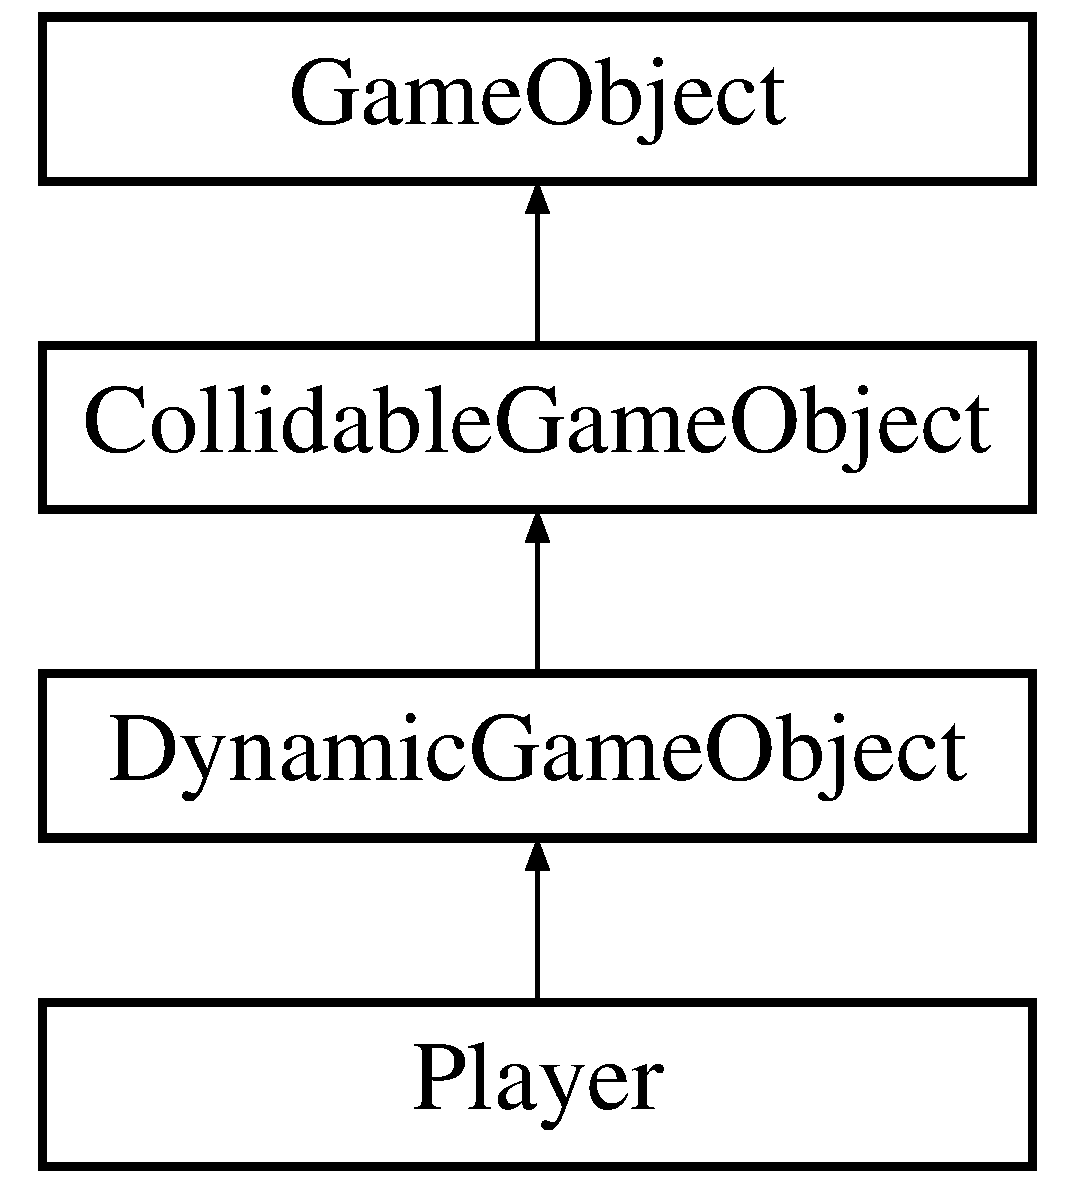
\includegraphics[height=4.000000cm]{class_player}
\end{center}
\end{figure}
\subsection*{Public Member Functions}
\begin{DoxyCompactItemize}
\item 
\hyperlink{class_player_a764ad06a52c68d38a95f61a731369c86}{Player} (\hyperlink{class_vector3}{Vector3} pos)
\item 
void \hyperlink{class_player_a72cc16348453f3a4b871eb2486c91497}{jump} (\hyperlink{class_vector3}{Vector3} jump\+Dir, float jump\+Speed)
\item 
void \hyperlink{class_player_a51e705a6ad3628144e02832d1839b360}{update} (int \hyperlink{_game_manager_8h_afea6a95c7a1c119b7106a4c735eb259d}{delta\+Time}) final
\item 
bool \hyperlink{class_player_a476948950b48fde97113707c1b6e6195}{collide\+With\+Bottom} (const \hyperlink{class_game_object}{Game\+Object} $\ast$other) const
\item 
void \hyperlink{class_player_a038a74bd768b6eec8fbe57cb2bacf811}{respawn} ()
\item 
void \hyperlink{class_player_a41f9e4a4e55ee3fc38614dcb965193a1}{restart\+Game} ()
\item 
void \hyperlink{class_player_a9098e6b411ea9102b02bb911eca6515b}{set\+Speed\+Multiplier} (float new\+Speed) final
\item 
void \hyperlink{class_player_a1fb512423a77eee4ed0dea7cb7179c83}{init} () final
\item 
void \hyperlink{class_player_a4da76233f59ad0254aa6ec533f9badcc}{render} () final
\end{DoxyCompactItemize}
\subsection*{Public Attributes}
\begin{DoxyCompactItemize}
\item 
\hyperlink{_player_8h_a3c730f37b1b3a893159bada67637fdb1}{Player\+State} \hyperlink{class_player_aea87fbb086b0cc358db8adf47bfa7369}{player\+State} = \hyperlink{_player_8h_a3c730f37b1b3a893159bada67637fdb1aefa0f3ce09b7d810dde1e3cde60f7c4f}{G\+R\+O\+U\+N\+D\+ED}
\item 
\hyperlink{class_vector3}{Vector3} \hyperlink{class_player_afef6386ca5fe8974bcc3d807b2261a09}{last\+Jump\+Dir} = \hyperlink{class_vector3}{Vector3}()
\item 
\hyperlink{class_vector3}{Vector3} \hyperlink{class_player_a6d0fe16db54a42ab13f0b8ed1ca0632c}{init\+Pos} = \hyperlink{class_vector3}{Vector3}()
\item 
int \hyperlink{class_player_a11d9ba38b586f5acfac4f2cd5233cbb4}{starting\+Lives} = 5
\item 
int \hyperlink{class_player_a6638b814a2cb74674b554d51a3e8a256}{current\+Lives} = \hyperlink{class_player_a11d9ba38b586f5acfac4f2cd5233cbb4}{starting\+Lives}
\end{DoxyCompactItemize}
\subsection*{Protected Attributes}
\begin{DoxyCompactItemize}
\item 
\hyperlink{class_vector3}{Vector3} \hyperlink{class_player_a9df1cbdc480439b69d82068b287ed071}{jump\+Target\+Pos} = \hyperlink{class_vector3}{Vector3}()
\item 
\hyperlink{class_vector3}{Vector3} \hyperlink{class_player_a6c51347e4c397febebd559c19d7969b9}{transition\+Pos} = \hyperlink{class_vector3}{Vector3}()
\item 
\hyperlink{class_vector3}{Vector3} \hyperlink{class_player_ab85f1fa829960281bfdf1171ecdbead7}{transition\+Jump\+Dir} = \hyperlink{class_vector3}{Vector3}()
\item 
float \hyperlink{class_player_af7711712d6bd0b3185f8a38f769ff3c8}{transition\+Jump\+Speed} = 0
\item 
\hyperlink{class_bounding_box}{Bounding\+Box} \hyperlink{class_player_ae86b1de018c7db9a201935a1a67e9ce0}{bottom\+Box} = \hyperlink{class_bounding_box}{Bounding\+Box}(\hyperlink{class_vector3}{Vector3}(0.\+1, -\/1, 0.\+1), \hyperlink{class_vector3}{Vector3}(0.\+9, 0, 0.\+9))
\end{DoxyCompactItemize}
\subsection*{Additional Inherited Members}


\subsection{Constructor \& Destructor Documentation}
\mbox{\Hypertarget{class_player_a764ad06a52c68d38a95f61a731369c86}\label{class_player_a764ad06a52c68d38a95f61a731369c86}} 
\index{Player@{Player}!Player@{Player}}
\index{Player@{Player}!Player@{Player}}
\subsubsection{\texorpdfstring{Player()}{Player()}}
{\footnotesize\ttfamily Player\+::\+Player (\begin{DoxyParamCaption}\item[{\hyperlink{class_vector3}{Vector3}}]{pos }\end{DoxyParamCaption})\hspace{0.3cm}{\ttfamily [inline]}}



\subsection{Member Function Documentation}
\mbox{\Hypertarget{class_player_a476948950b48fde97113707c1b6e6195}\label{class_player_a476948950b48fde97113707c1b6e6195}} 
\index{Player@{Player}!collide\+With\+Bottom@{collide\+With\+Bottom}}
\index{collide\+With\+Bottom@{collide\+With\+Bottom}!Player@{Player}}
\subsubsection{\texorpdfstring{collide\+With\+Bottom()}{collideWithBottom()}}
{\footnotesize\ttfamily bool Player\+::collide\+With\+Bottom (\begin{DoxyParamCaption}\item[{const \hyperlink{class_game_object}{Game\+Object} $\ast$}]{other }\end{DoxyParamCaption}) const\hspace{0.3cm}{\ttfamily [inline]}}

\mbox{\Hypertarget{class_player_a1fb512423a77eee4ed0dea7cb7179c83}\label{class_player_a1fb512423a77eee4ed0dea7cb7179c83}} 
\index{Player@{Player}!init@{init}}
\index{init@{init}!Player@{Player}}
\subsubsection{\texorpdfstring{init()}{init()}}
{\footnotesize\ttfamily void Player\+::init (\begin{DoxyParamCaption}{ }\end{DoxyParamCaption})\hspace{0.3cm}{\ttfamily [inline]}, {\ttfamily [final]}, {\ttfamily [virtual]}}



Reimplemented from \hyperlink{class_game_object_aecb2c1b9f69715d854f7604d5d7978ec}{Game\+Object}.

\mbox{\Hypertarget{class_player_a72cc16348453f3a4b871eb2486c91497}\label{class_player_a72cc16348453f3a4b871eb2486c91497}} 
\index{Player@{Player}!jump@{jump}}
\index{jump@{jump}!Player@{Player}}
\subsubsection{\texorpdfstring{jump()}{jump()}}
{\footnotesize\ttfamily void Player\+::jump (\begin{DoxyParamCaption}\item[{\hyperlink{class_vector3}{Vector3}}]{jump\+Dir,  }\item[{float}]{jump\+Speed }\end{DoxyParamCaption})\hspace{0.3cm}{\ttfamily [inline]}}

\mbox{\Hypertarget{class_player_a4da76233f59ad0254aa6ec533f9badcc}\label{class_player_a4da76233f59ad0254aa6ec533f9badcc}} 
\index{Player@{Player}!render@{render}}
\index{render@{render}!Player@{Player}}
\subsubsection{\texorpdfstring{render()}{render()}}
{\footnotesize\ttfamily void Player\+::render (\begin{DoxyParamCaption}{ }\end{DoxyParamCaption})\hspace{0.3cm}{\ttfamily [inline]}, {\ttfamily [final]}, {\ttfamily [virtual]}}



Reimplemented from \hyperlink{class_game_object_a484efb66a7a27c101e84c11d9905d7a6}{Game\+Object}.

\mbox{\Hypertarget{class_player_a038a74bd768b6eec8fbe57cb2bacf811}\label{class_player_a038a74bd768b6eec8fbe57cb2bacf811}} 
\index{Player@{Player}!respawn@{respawn}}
\index{respawn@{respawn}!Player@{Player}}
\subsubsection{\texorpdfstring{respawn()}{respawn()}}
{\footnotesize\ttfamily void Player\+::respawn (\begin{DoxyParamCaption}{ }\end{DoxyParamCaption})\hspace{0.3cm}{\ttfamily [inline]}}

\mbox{\Hypertarget{class_player_a41f9e4a4e55ee3fc38614dcb965193a1}\label{class_player_a41f9e4a4e55ee3fc38614dcb965193a1}} 
\index{Player@{Player}!restart\+Game@{restart\+Game}}
\index{restart\+Game@{restart\+Game}!Player@{Player}}
\subsubsection{\texorpdfstring{restart\+Game()}{restartGame()}}
{\footnotesize\ttfamily void Player\+::restart\+Game (\begin{DoxyParamCaption}{ }\end{DoxyParamCaption})\hspace{0.3cm}{\ttfamily [inline]}}

\mbox{\Hypertarget{class_player_a9098e6b411ea9102b02bb911eca6515b}\label{class_player_a9098e6b411ea9102b02bb911eca6515b}} 
\index{Player@{Player}!set\+Speed\+Multiplier@{set\+Speed\+Multiplier}}
\index{set\+Speed\+Multiplier@{set\+Speed\+Multiplier}!Player@{Player}}
\subsubsection{\texorpdfstring{set\+Speed\+Multiplier()}{setSpeedMultiplier()}}
{\footnotesize\ttfamily void Player\+::set\+Speed\+Multiplier (\begin{DoxyParamCaption}\item[{float}]{new\+Speed }\end{DoxyParamCaption})\hspace{0.3cm}{\ttfamily [inline]}, {\ttfamily [final]}, {\ttfamily [virtual]}}



Reimplemented from \hyperlink{class_dynamic_game_object_a7bf254357b0d2491044d175afdc36ca4}{Dynamic\+Game\+Object}.

\mbox{\Hypertarget{class_player_a51e705a6ad3628144e02832d1839b360}\label{class_player_a51e705a6ad3628144e02832d1839b360}} 
\index{Player@{Player}!update@{update}}
\index{update@{update}!Player@{Player}}
\subsubsection{\texorpdfstring{update()}{update()}}
{\footnotesize\ttfamily void Player\+::update (\begin{DoxyParamCaption}\item[{int}]{delta\+Time }\end{DoxyParamCaption})\hspace{0.3cm}{\ttfamily [inline]}, {\ttfamily [final]}, {\ttfamily [virtual]}}



Reimplemented from \hyperlink{class_dynamic_game_object_aaa505b57d131bbbce44d500ec2ca0e83}{Dynamic\+Game\+Object}.



\subsection{Member Data Documentation}
\mbox{\Hypertarget{class_player_ae86b1de018c7db9a201935a1a67e9ce0}\label{class_player_ae86b1de018c7db9a201935a1a67e9ce0}} 
\index{Player@{Player}!bottom\+Box@{bottom\+Box}}
\index{bottom\+Box@{bottom\+Box}!Player@{Player}}
\subsubsection{\texorpdfstring{bottom\+Box}{bottomBox}}
{\footnotesize\ttfamily \hyperlink{class_bounding_box}{Bounding\+Box} Player\+::bottom\+Box = \hyperlink{class_bounding_box}{Bounding\+Box}(\hyperlink{class_vector3}{Vector3}(0.\+1, -\/1, 0.\+1), \hyperlink{class_vector3}{Vector3}(0.\+9, 0, 0.\+9))\hspace{0.3cm}{\ttfamily [protected]}}

\mbox{\Hypertarget{class_player_a6638b814a2cb74674b554d51a3e8a256}\label{class_player_a6638b814a2cb74674b554d51a3e8a256}} 
\index{Player@{Player}!current\+Lives@{current\+Lives}}
\index{current\+Lives@{current\+Lives}!Player@{Player}}
\subsubsection{\texorpdfstring{current\+Lives}{currentLives}}
{\footnotesize\ttfamily int Player\+::current\+Lives = \hyperlink{class_player_a11d9ba38b586f5acfac4f2cd5233cbb4}{starting\+Lives}}

\mbox{\Hypertarget{class_player_a6d0fe16db54a42ab13f0b8ed1ca0632c}\label{class_player_a6d0fe16db54a42ab13f0b8ed1ca0632c}} 
\index{Player@{Player}!init\+Pos@{init\+Pos}}
\index{init\+Pos@{init\+Pos}!Player@{Player}}
\subsubsection{\texorpdfstring{init\+Pos}{initPos}}
{\footnotesize\ttfamily \hyperlink{class_vector3}{Vector3} Player\+::init\+Pos = \hyperlink{class_vector3}{Vector3}()}

\mbox{\Hypertarget{class_player_a9df1cbdc480439b69d82068b287ed071}\label{class_player_a9df1cbdc480439b69d82068b287ed071}} 
\index{Player@{Player}!jump\+Target\+Pos@{jump\+Target\+Pos}}
\index{jump\+Target\+Pos@{jump\+Target\+Pos}!Player@{Player}}
\subsubsection{\texorpdfstring{jump\+Target\+Pos}{jumpTargetPos}}
{\footnotesize\ttfamily \hyperlink{class_vector3}{Vector3} Player\+::jump\+Target\+Pos = \hyperlink{class_vector3}{Vector3}()\hspace{0.3cm}{\ttfamily [protected]}}

\mbox{\Hypertarget{class_player_afef6386ca5fe8974bcc3d807b2261a09}\label{class_player_afef6386ca5fe8974bcc3d807b2261a09}} 
\index{Player@{Player}!last\+Jump\+Dir@{last\+Jump\+Dir}}
\index{last\+Jump\+Dir@{last\+Jump\+Dir}!Player@{Player}}
\subsubsection{\texorpdfstring{last\+Jump\+Dir}{lastJumpDir}}
{\footnotesize\ttfamily \hyperlink{class_vector3}{Vector3} Player\+::last\+Jump\+Dir = \hyperlink{class_vector3}{Vector3}()}

\mbox{\Hypertarget{class_player_aea87fbb086b0cc358db8adf47bfa7369}\label{class_player_aea87fbb086b0cc358db8adf47bfa7369}} 
\index{Player@{Player}!player\+State@{player\+State}}
\index{player\+State@{player\+State}!Player@{Player}}
\subsubsection{\texorpdfstring{player\+State}{playerState}}
{\footnotesize\ttfamily \hyperlink{_player_8h_a3c730f37b1b3a893159bada67637fdb1}{Player\+State} Player\+::player\+State = \hyperlink{_player_8h_a3c730f37b1b3a893159bada67637fdb1aefa0f3ce09b7d810dde1e3cde60f7c4f}{G\+R\+O\+U\+N\+D\+ED}}

\mbox{\Hypertarget{class_player_a11d9ba38b586f5acfac4f2cd5233cbb4}\label{class_player_a11d9ba38b586f5acfac4f2cd5233cbb4}} 
\index{Player@{Player}!starting\+Lives@{starting\+Lives}}
\index{starting\+Lives@{starting\+Lives}!Player@{Player}}
\subsubsection{\texorpdfstring{starting\+Lives}{startingLives}}
{\footnotesize\ttfamily int Player\+::starting\+Lives = 5}

\mbox{\Hypertarget{class_player_ab85f1fa829960281bfdf1171ecdbead7}\label{class_player_ab85f1fa829960281bfdf1171ecdbead7}} 
\index{Player@{Player}!transition\+Jump\+Dir@{transition\+Jump\+Dir}}
\index{transition\+Jump\+Dir@{transition\+Jump\+Dir}!Player@{Player}}
\subsubsection{\texorpdfstring{transition\+Jump\+Dir}{transitionJumpDir}}
{\footnotesize\ttfamily \hyperlink{class_vector3}{Vector3} Player\+::transition\+Jump\+Dir = \hyperlink{class_vector3}{Vector3}()\hspace{0.3cm}{\ttfamily [protected]}}

\mbox{\Hypertarget{class_player_af7711712d6bd0b3185f8a38f769ff3c8}\label{class_player_af7711712d6bd0b3185f8a38f769ff3c8}} 
\index{Player@{Player}!transition\+Jump\+Speed@{transition\+Jump\+Speed}}
\index{transition\+Jump\+Speed@{transition\+Jump\+Speed}!Player@{Player}}
\subsubsection{\texorpdfstring{transition\+Jump\+Speed}{transitionJumpSpeed}}
{\footnotesize\ttfamily float Player\+::transition\+Jump\+Speed = 0\hspace{0.3cm}{\ttfamily [protected]}}

\mbox{\Hypertarget{class_player_a6c51347e4c397febebd559c19d7969b9}\label{class_player_a6c51347e4c397febebd559c19d7969b9}} 
\index{Player@{Player}!transition\+Pos@{transition\+Pos}}
\index{transition\+Pos@{transition\+Pos}!Player@{Player}}
\subsubsection{\texorpdfstring{transition\+Pos}{transitionPos}}
{\footnotesize\ttfamily \hyperlink{class_vector3}{Vector3} Player\+::transition\+Pos = \hyperlink{class_vector3}{Vector3}()\hspace{0.3cm}{\ttfamily [protected]}}



The documentation for this class was generated from the following file\+:\begin{DoxyCompactItemize}
\item 
/\+Users/matya/\+A\+V\+T7/src/objects/\hyperlink{_player_8h}{Player.\+h}\end{DoxyCompactItemize}

\hypertarget{class_point_light}{}\section{Point\+Light Class Reference}
\label{class_point_light}\index{Point\+Light@{Point\+Light}}


{\ttfamily \#include $<$Point\+Light.\+h$>$}

Inheritance diagram for Point\+Light\+:\begin{figure}[H]
\begin{center}
\leavevmode
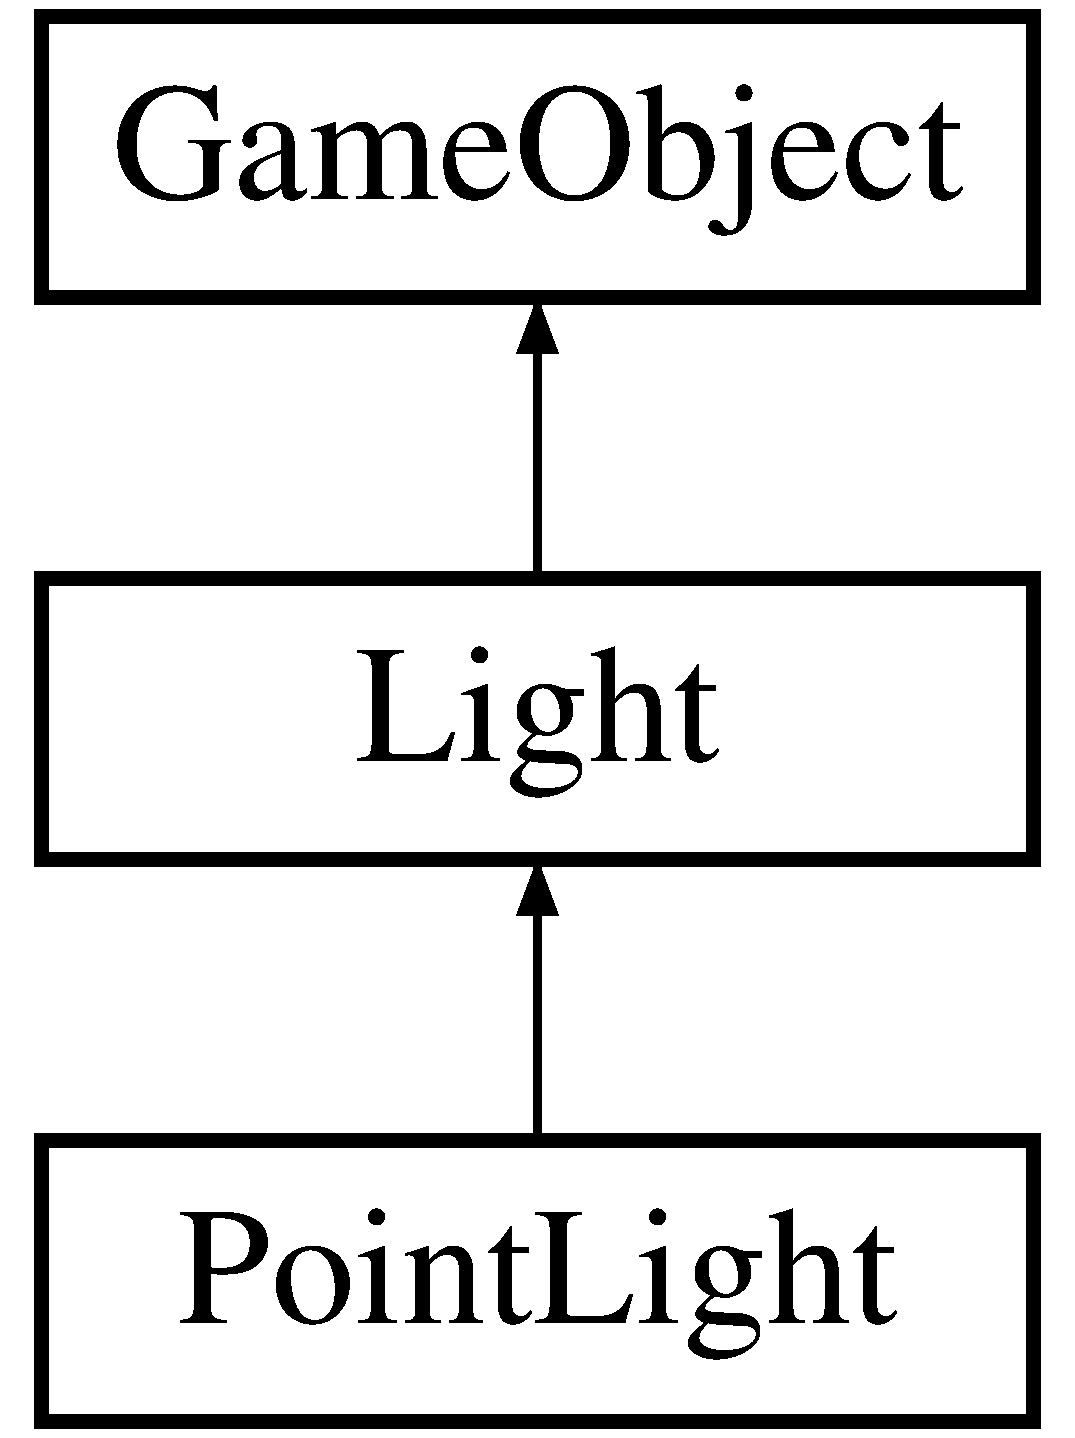
\includegraphics[height=3.000000cm]{class_point_light}
\end{center}
\end{figure}
\subsection*{Public Member Functions}
\begin{DoxyCompactItemize}
\item 
\hyperlink{class_point_light_af6171c3cdf01dca3c900e14fee5300fe}{Point\+Light} (\hyperlink{class_vector3}{Vector3} pos, int \hyperlink{class_light_ae0028340ad3a9f2e196b68365d5fe972}{light\+\_\+id}, bool light\+\_\+active=true)
\item 
void \hyperlink{class_point_light_a4584cb5e40e5dd6ab2f43ec84851152c}{render} () final
\end{DoxyCompactItemize}
\subsection*{Additional Inherited Members}


\subsection{Constructor \& Destructor Documentation}
\mbox{\Hypertarget{class_point_light_af6171c3cdf01dca3c900e14fee5300fe}\label{class_point_light_af6171c3cdf01dca3c900e14fee5300fe}} 
\index{Point\+Light@{Point\+Light}!Point\+Light@{Point\+Light}}
\index{Point\+Light@{Point\+Light}!Point\+Light@{Point\+Light}}
\subsubsection{\texorpdfstring{Point\+Light()}{PointLight()}}
{\footnotesize\ttfamily Point\+Light\+::\+Point\+Light (\begin{DoxyParamCaption}\item[{\hyperlink{class_vector3}{Vector3}}]{pos,  }\item[{int}]{light\+\_\+id,  }\item[{bool}]{light\+\_\+active = {\ttfamily true} }\end{DoxyParamCaption})\hspace{0.3cm}{\ttfamily [inline]}}



\subsection{Member Function Documentation}
\mbox{\Hypertarget{class_point_light_a4584cb5e40e5dd6ab2f43ec84851152c}\label{class_point_light_a4584cb5e40e5dd6ab2f43ec84851152c}} 
\index{Point\+Light@{Point\+Light}!render@{render}}
\index{render@{render}!Point\+Light@{Point\+Light}}
\subsubsection{\texorpdfstring{render()}{render()}}
{\footnotesize\ttfamily void Point\+Light\+::render (\begin{DoxyParamCaption}{ }\end{DoxyParamCaption})\hspace{0.3cm}{\ttfamily [inline]}, {\ttfamily [final]}, {\ttfamily [virtual]}}



Reimplemented from \hyperlink{class_game_object_a484efb66a7a27c101e84c11d9905d7a6}{Game\+Object}.



The documentation for this class was generated from the following file\+:\begin{DoxyCompactItemize}
\item 
/\+Users/matya/\+A\+V\+T7/src/objects/\hyperlink{_point_light_8h}{Point\+Light.\+h}\end{DoxyCompactItemize}

\hypertarget{class_river}{}\section{River Class Reference}
\label{class_river}\index{River@{River}}


{\ttfamily \#include $<$River.\+h$>$}

Inheritance diagram for River\+:\begin{figure}[H]
\begin{center}
\leavevmode
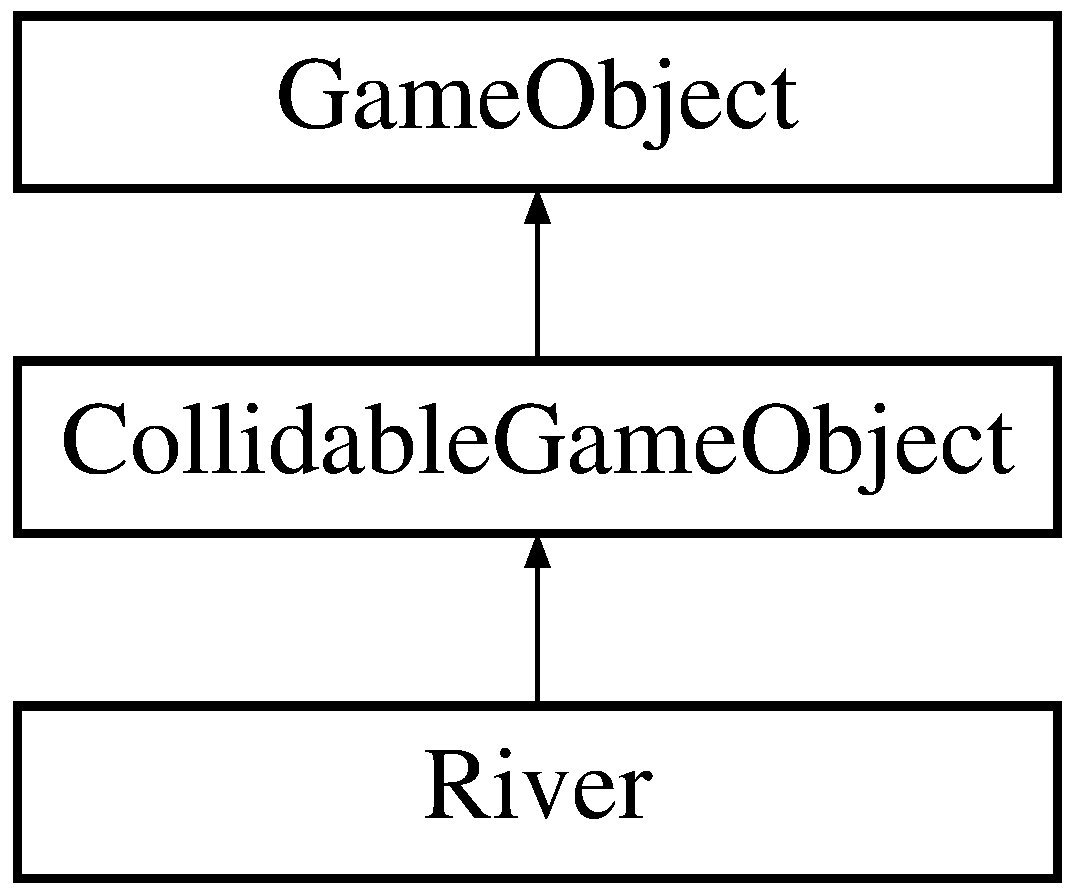
\includegraphics[height=3.000000cm]{class_river}
\end{center}
\end{figure}
\subsection*{Public Member Functions}
\begin{DoxyCompactItemize}
\item 
\hyperlink{class_river_a305d3ec8496a5373328045da3b8d8362}{River} ()
\item 
void \hyperlink{class_river_a34d39d986e411f957e77e85ba5719af4}{init} ()
\item 
void \hyperlink{class_river_abf5ba1cc4356fbf57059da23e3a1997a}{render} ()
\end{DoxyCompactItemize}
\subsection*{Additional Inherited Members}


\subsection{Constructor \& Destructor Documentation}
\mbox{\Hypertarget{class_river_a305d3ec8496a5373328045da3b8d8362}\label{class_river_a305d3ec8496a5373328045da3b8d8362}} 
\index{River@{River}!River@{River}}
\index{River@{River}!River@{River}}
\subsubsection{\texorpdfstring{River()}{River()}}
{\footnotesize\ttfamily River\+::\+River (\begin{DoxyParamCaption}{ }\end{DoxyParamCaption})\hspace{0.3cm}{\ttfamily [inline]}}



\subsection{Member Function Documentation}
\mbox{\Hypertarget{class_river_a34d39d986e411f957e77e85ba5719af4}\label{class_river_a34d39d986e411f957e77e85ba5719af4}} 
\index{River@{River}!init@{init}}
\index{init@{init}!River@{River}}
\subsubsection{\texorpdfstring{init()}{init()}}
{\footnotesize\ttfamily void River\+::init (\begin{DoxyParamCaption}{ }\end{DoxyParamCaption})\hspace{0.3cm}{\ttfamily [inline]}, {\ttfamily [virtual]}}



Reimplemented from \hyperlink{class_game_object_aecb2c1b9f69715d854f7604d5d7978ec}{Game\+Object}.

\mbox{\Hypertarget{class_river_abf5ba1cc4356fbf57059da23e3a1997a}\label{class_river_abf5ba1cc4356fbf57059da23e3a1997a}} 
\index{River@{River}!render@{render}}
\index{render@{render}!River@{River}}
\subsubsection{\texorpdfstring{render()}{render()}}
{\footnotesize\ttfamily void River\+::render (\begin{DoxyParamCaption}{ }\end{DoxyParamCaption})\hspace{0.3cm}{\ttfamily [inline]}, {\ttfamily [virtual]}}



Reimplemented from \hyperlink{class_game_object_a484efb66a7a27c101e84c11d9905d7a6}{Game\+Object}.



The documentation for this class was generated from the following file\+:\begin{DoxyCompactItemize}
\item 
/\+Users/matya/\+A\+V\+T7/src/objects/\hyperlink{_river_8h}{River.\+h}\end{DoxyCompactItemize}

\hypertarget{class_road}{}\section{Road Class Reference}
\label{class_road}\index{Road@{Road}}


{\ttfamily \#include $<$Road.\+h$>$}

Inheritance diagram for Road\+:\begin{figure}[H]
\begin{center}
\leavevmode
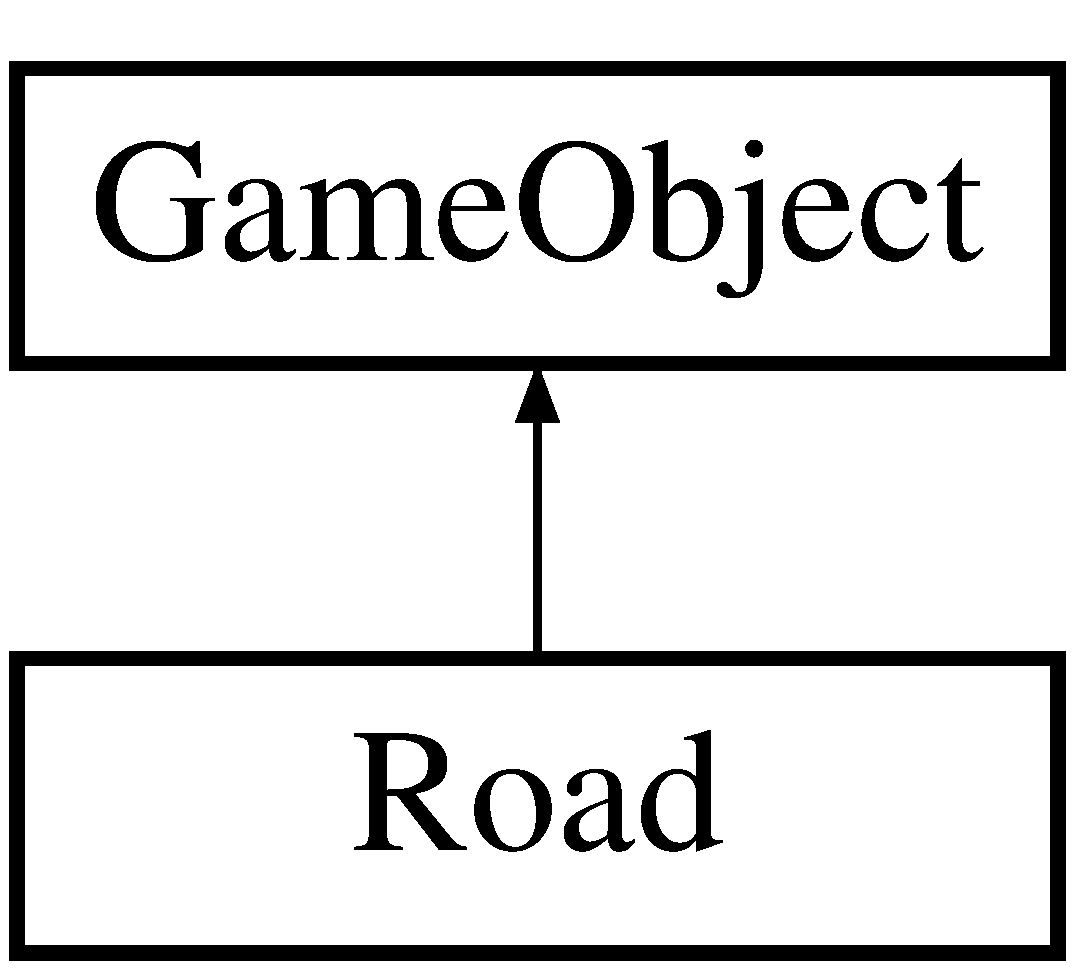
\includegraphics[height=2.000000cm]{class_road}
\end{center}
\end{figure}
\subsection*{Public Member Functions}
\begin{DoxyCompactItemize}
\item 
\hyperlink{class_road_a90bb6be2a5c3b6997849a915e2af0cf0}{Road} ()
\item 
void \hyperlink{class_road_a2d72b47fce205751e504929e91a7e567}{init} () override
\item 
void \hyperlink{class_road_a2ca4cc3c6043f6d1044992073e9fe3ba}{render} () override
\end{DoxyCompactItemize}
\subsection*{Additional Inherited Members}


\subsection{Constructor \& Destructor Documentation}
\mbox{\Hypertarget{class_road_a90bb6be2a5c3b6997849a915e2af0cf0}\label{class_road_a90bb6be2a5c3b6997849a915e2af0cf0}} 
\index{Road@{Road}!Road@{Road}}
\index{Road@{Road}!Road@{Road}}
\subsubsection{\texorpdfstring{Road()}{Road()}}
{\footnotesize\ttfamily Road\+::\+Road (\begin{DoxyParamCaption}{ }\end{DoxyParamCaption})\hspace{0.3cm}{\ttfamily [inline]}}



\subsection{Member Function Documentation}
\mbox{\Hypertarget{class_road_a2d72b47fce205751e504929e91a7e567}\label{class_road_a2d72b47fce205751e504929e91a7e567}} 
\index{Road@{Road}!init@{init}}
\index{init@{init}!Road@{Road}}
\subsubsection{\texorpdfstring{init()}{init()}}
{\footnotesize\ttfamily void Road\+::init (\begin{DoxyParamCaption}{ }\end{DoxyParamCaption})\hspace{0.3cm}{\ttfamily [inline]}, {\ttfamily [override]}, {\ttfamily [virtual]}}



Reimplemented from \hyperlink{class_game_object_aecb2c1b9f69715d854f7604d5d7978ec}{Game\+Object}.

\mbox{\Hypertarget{class_road_a2ca4cc3c6043f6d1044992073e9fe3ba}\label{class_road_a2ca4cc3c6043f6d1044992073e9fe3ba}} 
\index{Road@{Road}!render@{render}}
\index{render@{render}!Road@{Road}}
\subsubsection{\texorpdfstring{render()}{render()}}
{\footnotesize\ttfamily void Road\+::render (\begin{DoxyParamCaption}{ }\end{DoxyParamCaption})\hspace{0.3cm}{\ttfamily [inline]}, {\ttfamily [override]}, {\ttfamily [virtual]}}



Reimplemented from \hyperlink{class_game_object_a484efb66a7a27c101e84c11d9905d7a6}{Game\+Object}.



The documentation for this class was generated from the following file\+:\begin{DoxyCompactItemize}
\item 
/\+Users/matya/\+A\+V\+T7/src/objects/\hyperlink{_road_8h}{Road.\+h}\end{DoxyCompactItemize}

\hypertarget{class_scene_collider}{}\section{Scene\+Collider Class Reference}
\label{class_scene_collider}\index{Scene\+Collider@{Scene\+Collider}}


{\ttfamily \#include $<$Scene\+Collider.\+h$>$}

Inheritance diagram for Scene\+Collider\+:\begin{figure}[H]
\begin{center}
\leavevmode
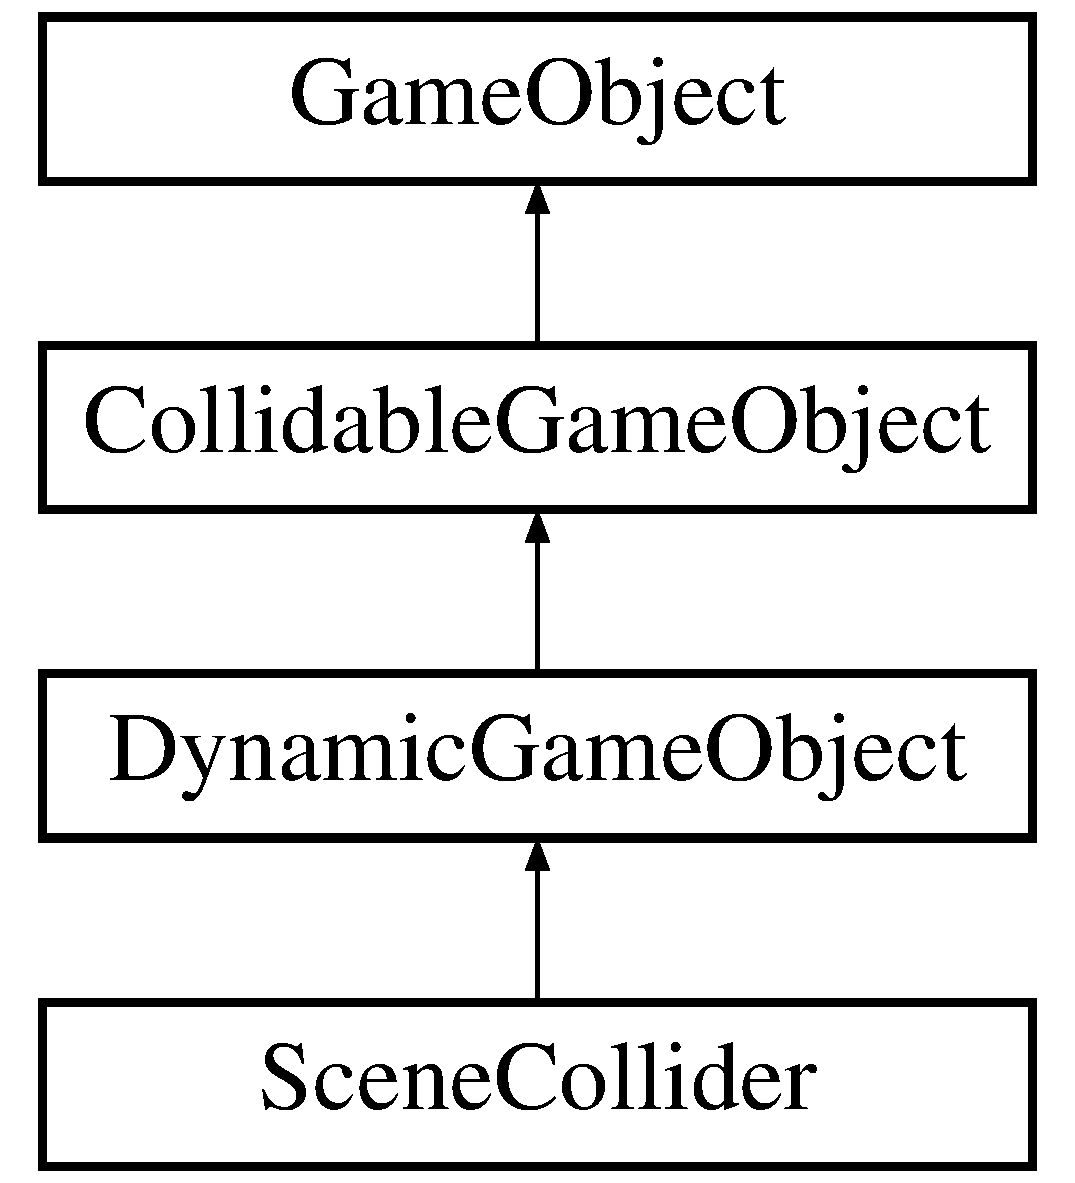
\includegraphics[height=4.000000cm]{class_scene_collider}
\end{center}
\end{figure}
\subsection*{Public Member Functions}
\begin{DoxyCompactItemize}
\item 
\hyperlink{class_scene_collider_a1694cf0e8d99751e9636fe98ebc81e61}{Scene\+Collider} (\hyperlink{class_vector3}{Vector3} pos)
\item 
void \hyperlink{class_scene_collider_a2b2aae1d24b6f40188150d3002e00218}{init} () override
\item 
void \hyperlink{class_scene_collider_aa46bbfb6657449115aa6855a8f46e3f5}{render} () override
\end{DoxyCompactItemize}
\subsection*{Additional Inherited Members}


\subsection{Constructor \& Destructor Documentation}
\mbox{\Hypertarget{class_scene_collider_a1694cf0e8d99751e9636fe98ebc81e61}\label{class_scene_collider_a1694cf0e8d99751e9636fe98ebc81e61}} 
\index{Scene\+Collider@{Scene\+Collider}!Scene\+Collider@{Scene\+Collider}}
\index{Scene\+Collider@{Scene\+Collider}!Scene\+Collider@{Scene\+Collider}}
\subsubsection{\texorpdfstring{Scene\+Collider()}{SceneCollider()}}
{\footnotesize\ttfamily Scene\+Collider\+::\+Scene\+Collider (\begin{DoxyParamCaption}\item[{\hyperlink{class_vector3}{Vector3}}]{pos }\end{DoxyParamCaption})\hspace{0.3cm}{\ttfamily [inline]}, {\ttfamily [explicit]}}



\subsection{Member Function Documentation}
\mbox{\Hypertarget{class_scene_collider_a2b2aae1d24b6f40188150d3002e00218}\label{class_scene_collider_a2b2aae1d24b6f40188150d3002e00218}} 
\index{Scene\+Collider@{Scene\+Collider}!init@{init}}
\index{init@{init}!Scene\+Collider@{Scene\+Collider}}
\subsubsection{\texorpdfstring{init()}{init()}}
{\footnotesize\ttfamily void Scene\+Collider\+::init (\begin{DoxyParamCaption}{ }\end{DoxyParamCaption})\hspace{0.3cm}{\ttfamily [inline]}, {\ttfamily [override]}, {\ttfamily [virtual]}}



Reimplemented from \hyperlink{class_game_object_aecb2c1b9f69715d854f7604d5d7978ec}{Game\+Object}.

\mbox{\Hypertarget{class_scene_collider_aa46bbfb6657449115aa6855a8f46e3f5}\label{class_scene_collider_aa46bbfb6657449115aa6855a8f46e3f5}} 
\index{Scene\+Collider@{Scene\+Collider}!render@{render}}
\index{render@{render}!Scene\+Collider@{Scene\+Collider}}
\subsubsection{\texorpdfstring{render()}{render()}}
{\footnotesize\ttfamily void Scene\+Collider\+::render (\begin{DoxyParamCaption}{ }\end{DoxyParamCaption})\hspace{0.3cm}{\ttfamily [inline]}, {\ttfamily [override]}, {\ttfamily [virtual]}}



Reimplemented from \hyperlink{class_game_object_a484efb66a7a27c101e84c11d9905d7a6}{Game\+Object}.



The documentation for this class was generated from the following file\+:\begin{DoxyCompactItemize}
\item 
/\+Users/matya/\+A\+V\+T7/src/objects/\hyperlink{_scene_collider_8h}{Scene\+Collider.\+h}\end{DoxyCompactItemize}

\hypertarget{struct_shader_indices}{}\section{Shader\+Indices Struct Reference}
\label{struct_shader_indices}\index{Shader\+Indices@{Shader\+Indices}}


{\ttfamily \#include $<$Shader\+Indices.\+h$>$}

\subsection*{Public Member Functions}
\begin{DoxyCompactItemize}
\item 
\hyperlink{struct_shader_indices_a1c4546e1ea7fc53b958d2be8b50aa3ce}{Shader\+Indices} (G\+Lint l\+\_\+amb, G\+Lint l\+\_\+dif, G\+Lint l\+\_\+spc, G\+Lint l\+\_\+shi)
\end{DoxyCompactItemize}
\subsection*{Public Attributes}
\begin{DoxyCompactItemize}
\item 
G\+Lint \hyperlink{struct_shader_indices_a7c0b0f9199914b3b6cd1944d41c609a3}{loc\+\_\+amb}
\item 
G\+Lint \hyperlink{struct_shader_indices_aa3df8d026b2faa1bc06e79618c86a77c}{loc\+\_\+dif}
\item 
G\+Lint \hyperlink{struct_shader_indices_a78c40b0a417042217c80c46d9a2b543a}{loc\+\_\+spc}
\item 
G\+Lint \hyperlink{struct_shader_indices_a09528fea691de3860ad75b63ec6a00bb}{loc\+\_\+shi}
\end{DoxyCompactItemize}


\subsection{Constructor \& Destructor Documentation}
\mbox{\Hypertarget{struct_shader_indices_a1c4546e1ea7fc53b958d2be8b50aa3ce}\label{struct_shader_indices_a1c4546e1ea7fc53b958d2be8b50aa3ce}} 
\index{Shader\+Indices@{Shader\+Indices}!Shader\+Indices@{Shader\+Indices}}
\index{Shader\+Indices@{Shader\+Indices}!Shader\+Indices@{Shader\+Indices}}
\subsubsection{\texorpdfstring{Shader\+Indices()}{ShaderIndices()}}
{\footnotesize\ttfamily Shader\+Indices\+::\+Shader\+Indices (\begin{DoxyParamCaption}\item[{G\+Lint}]{l\+\_\+amb,  }\item[{G\+Lint}]{l\+\_\+dif,  }\item[{G\+Lint}]{l\+\_\+spc,  }\item[{G\+Lint}]{l\+\_\+shi }\end{DoxyParamCaption})\hspace{0.3cm}{\ttfamily [inline]}}



\subsection{Member Data Documentation}
\mbox{\Hypertarget{struct_shader_indices_a7c0b0f9199914b3b6cd1944d41c609a3}\label{struct_shader_indices_a7c0b0f9199914b3b6cd1944d41c609a3}} 
\index{Shader\+Indices@{Shader\+Indices}!loc\+\_\+amb@{loc\+\_\+amb}}
\index{loc\+\_\+amb@{loc\+\_\+amb}!Shader\+Indices@{Shader\+Indices}}
\subsubsection{\texorpdfstring{loc\+\_\+amb}{loc\_amb}}
{\footnotesize\ttfamily G\+Lint Shader\+Indices\+::loc\+\_\+amb}

\mbox{\Hypertarget{struct_shader_indices_aa3df8d026b2faa1bc06e79618c86a77c}\label{struct_shader_indices_aa3df8d026b2faa1bc06e79618c86a77c}} 
\index{Shader\+Indices@{Shader\+Indices}!loc\+\_\+dif@{loc\+\_\+dif}}
\index{loc\+\_\+dif@{loc\+\_\+dif}!Shader\+Indices@{Shader\+Indices}}
\subsubsection{\texorpdfstring{loc\+\_\+dif}{loc\_dif}}
{\footnotesize\ttfamily G\+Lint Shader\+Indices\+::loc\+\_\+dif}

\mbox{\Hypertarget{struct_shader_indices_a09528fea691de3860ad75b63ec6a00bb}\label{struct_shader_indices_a09528fea691de3860ad75b63ec6a00bb}} 
\index{Shader\+Indices@{Shader\+Indices}!loc\+\_\+shi@{loc\+\_\+shi}}
\index{loc\+\_\+shi@{loc\+\_\+shi}!Shader\+Indices@{Shader\+Indices}}
\subsubsection{\texorpdfstring{loc\+\_\+shi}{loc\_shi}}
{\footnotesize\ttfamily G\+Lint Shader\+Indices\+::loc\+\_\+shi}

\mbox{\Hypertarget{struct_shader_indices_a78c40b0a417042217c80c46d9a2b543a}\label{struct_shader_indices_a78c40b0a417042217c80c46d9a2b543a}} 
\index{Shader\+Indices@{Shader\+Indices}!loc\+\_\+spc@{loc\+\_\+spc}}
\index{loc\+\_\+spc@{loc\+\_\+spc}!Shader\+Indices@{Shader\+Indices}}
\subsubsection{\texorpdfstring{loc\+\_\+spc}{loc\_spc}}
{\footnotesize\ttfamily G\+Lint Shader\+Indices\+::loc\+\_\+spc}



The documentation for this struct was generated from the following file\+:\begin{DoxyCompactItemize}
\item 
/\+Users/matya/\+A\+V\+T7/src/\hyperlink{_shader_indices_8h}{Shader\+Indices.\+h}\end{DoxyCompactItemize}

\hypertarget{class_sidewalls}{}\section{Sidewalls Class Reference}
\label{class_sidewalls}\index{Sidewalls@{Sidewalls}}


{\ttfamily \#include $<$Sidewalls.\+h$>$}

Inheritance diagram for Sidewalls\+:\begin{figure}[H]
\begin{center}
\leavevmode
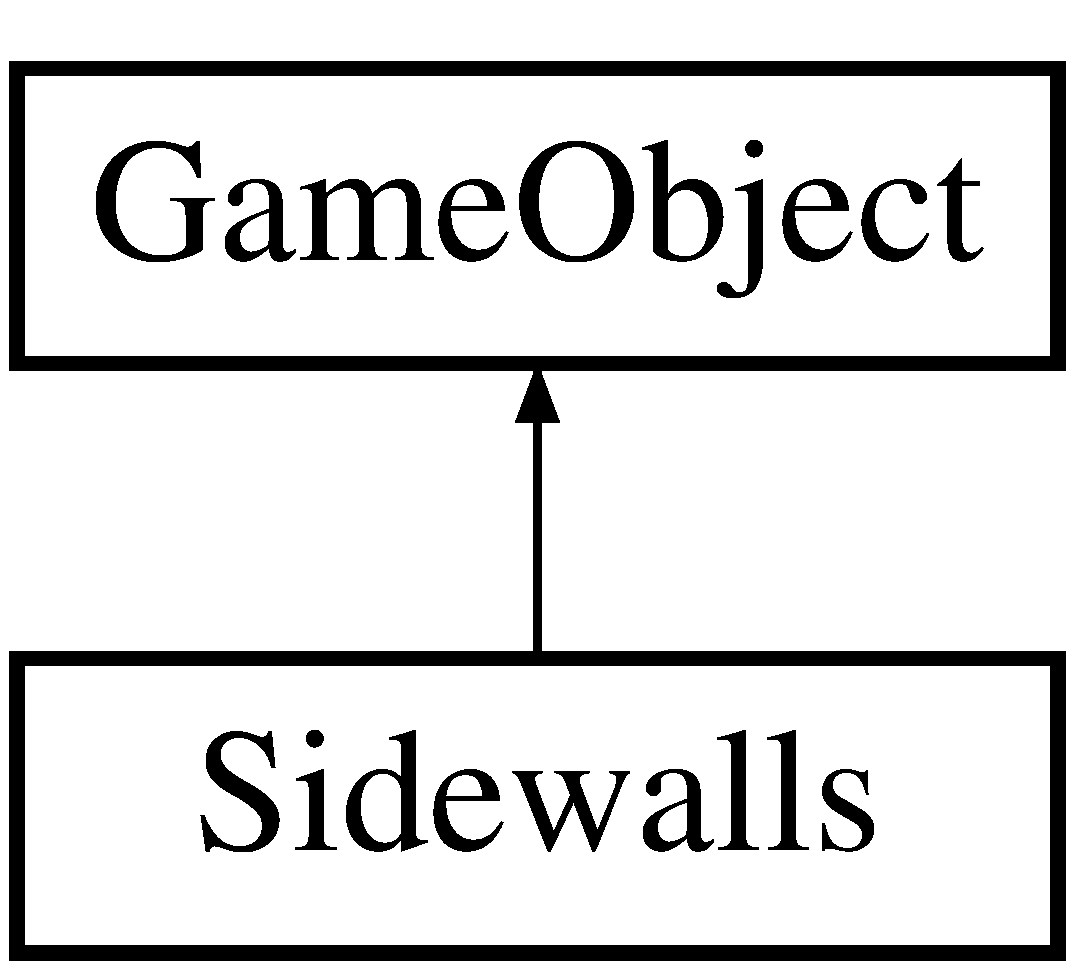
\includegraphics[height=2.000000cm]{class_sidewalls}
\end{center}
\end{figure}
\subsection*{Public Member Functions}
\begin{DoxyCompactItemize}
\item 
\hyperlink{class_sidewalls_aa5ac48e449af6ce0c65d37d452b64d7a}{Sidewalls} ()
\item 
void \hyperlink{class_sidewalls_a4d6161bfb13fe2779a9510c424879707}{init} () override
\item 
void \hyperlink{class_sidewalls_a3459ee5dee7a73043955607c5cb51d73}{render} () override
\end{DoxyCompactItemize}
\subsection*{Additional Inherited Members}


\subsection{Constructor \& Destructor Documentation}
\mbox{\Hypertarget{class_sidewalls_aa5ac48e449af6ce0c65d37d452b64d7a}\label{class_sidewalls_aa5ac48e449af6ce0c65d37d452b64d7a}} 
\index{Sidewalls@{Sidewalls}!Sidewalls@{Sidewalls}}
\index{Sidewalls@{Sidewalls}!Sidewalls@{Sidewalls}}
\subsubsection{\texorpdfstring{Sidewalls()}{Sidewalls()}}
{\footnotesize\ttfamily Sidewalls\+::\+Sidewalls (\begin{DoxyParamCaption}{ }\end{DoxyParamCaption})\hspace{0.3cm}{\ttfamily [inline]}, {\ttfamily [explicit]}}



\subsection{Member Function Documentation}
\mbox{\Hypertarget{class_sidewalls_a4d6161bfb13fe2779a9510c424879707}\label{class_sidewalls_a4d6161bfb13fe2779a9510c424879707}} 
\index{Sidewalls@{Sidewalls}!init@{init}}
\index{init@{init}!Sidewalls@{Sidewalls}}
\subsubsection{\texorpdfstring{init()}{init()}}
{\footnotesize\ttfamily void Sidewalls\+::init (\begin{DoxyParamCaption}{ }\end{DoxyParamCaption})\hspace{0.3cm}{\ttfamily [inline]}, {\ttfamily [override]}, {\ttfamily [virtual]}}



Reimplemented from \hyperlink{class_game_object_aecb2c1b9f69715d854f7604d5d7978ec}{Game\+Object}.

\mbox{\Hypertarget{class_sidewalls_a3459ee5dee7a73043955607c5cb51d73}\label{class_sidewalls_a3459ee5dee7a73043955607c5cb51d73}} 
\index{Sidewalls@{Sidewalls}!render@{render}}
\index{render@{render}!Sidewalls@{Sidewalls}}
\subsubsection{\texorpdfstring{render()}{render()}}
{\footnotesize\ttfamily void Sidewalls\+::render (\begin{DoxyParamCaption}{ }\end{DoxyParamCaption})\hspace{0.3cm}{\ttfamily [inline]}, {\ttfamily [override]}, {\ttfamily [virtual]}}



Reimplemented from \hyperlink{class_game_object_a484efb66a7a27c101e84c11d9905d7a6}{Game\+Object}.



The documentation for this class was generated from the following file\+:\begin{DoxyCompactItemize}
\item 
/\+Users/matya/\+A\+V\+T7/src/objects/\hyperlink{_sidewalls_8h}{Sidewalls.\+h}\end{DoxyCompactItemize}

\hypertarget{class_spot_light}{}\section{Spot\+Light Class Reference}
\label{class_spot_light}\index{Spot\+Light@{Spot\+Light}}


{\ttfamily \#include $<$Spot\+Light.\+h$>$}

Inheritance diagram for Spot\+Light\+:\begin{figure}[H]
\begin{center}
\leavevmode
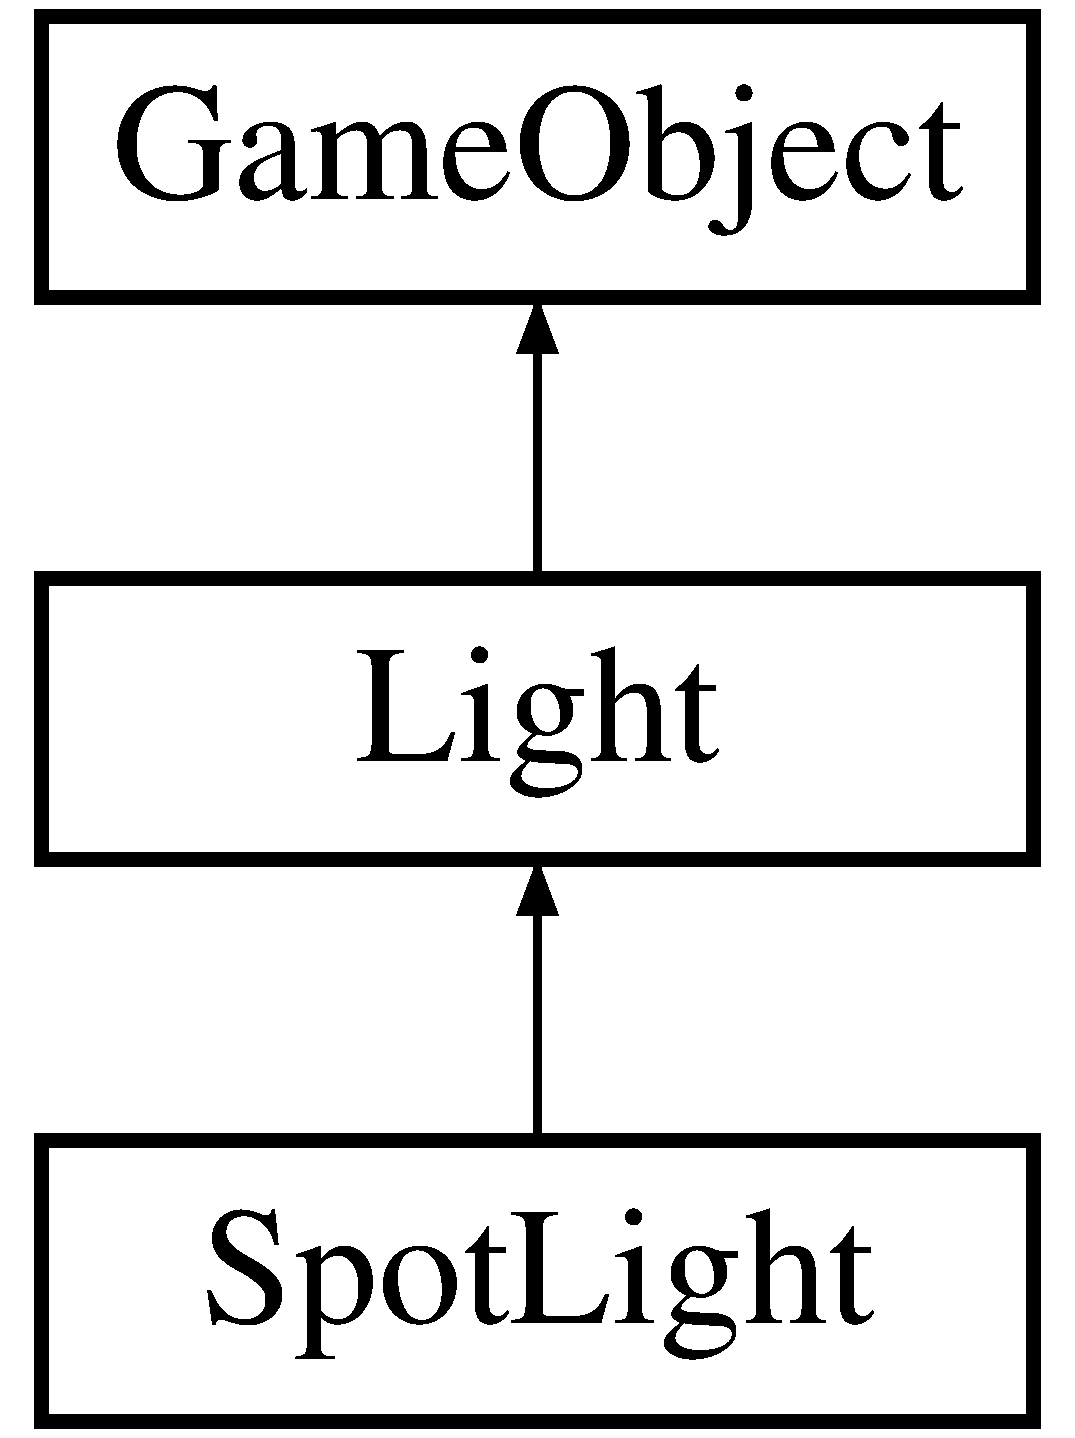
\includegraphics[height=3.000000cm]{class_spot_light}
\end{center}
\end{figure}
\subsection*{Public Member Functions}
\begin{DoxyCompactItemize}
\item 
\hyperlink{class_spot_light_a2e1f999d7325c5d6d5cc0d5f4c58e447}{Spot\+Light} (\hyperlink{class_vector3}{Vector3} pos, \hyperlink{class_vector3}{Vector3} dir, int \hyperlink{class_light_ae0028340ad3a9f2e196b68365d5fe972}{light\+\_\+id}, bool light\+\_\+active=true)
\item 
void \hyperlink{class_spot_light_a05dc942328210344caff20ffd58d0eb6}{render} () final
\end{DoxyCompactItemize}
\subsection*{Public Attributes}
\begin{DoxyCompactItemize}
\item 
\hyperlink{class_vector3}{Vector3} \hyperlink{class_spot_light_a105b6a5c34c8ee65a822a84090c26ba1}{light\+\_\+dir}
\end{DoxyCompactItemize}
\subsection*{Additional Inherited Members}


\subsection{Constructor \& Destructor Documentation}
\mbox{\Hypertarget{class_spot_light_a2e1f999d7325c5d6d5cc0d5f4c58e447}\label{class_spot_light_a2e1f999d7325c5d6d5cc0d5f4c58e447}} 
\index{Spot\+Light@{Spot\+Light}!Spot\+Light@{Spot\+Light}}
\index{Spot\+Light@{Spot\+Light}!Spot\+Light@{Spot\+Light}}
\subsubsection{\texorpdfstring{Spot\+Light()}{SpotLight()}}
{\footnotesize\ttfamily Spot\+Light\+::\+Spot\+Light (\begin{DoxyParamCaption}\item[{\hyperlink{class_vector3}{Vector3}}]{pos,  }\item[{\hyperlink{class_vector3}{Vector3}}]{dir,  }\item[{int}]{light\+\_\+id,  }\item[{bool}]{light\+\_\+active = {\ttfamily true} }\end{DoxyParamCaption})\hspace{0.3cm}{\ttfamily [inline]}}



\subsection{Member Function Documentation}
\mbox{\Hypertarget{class_spot_light_a05dc942328210344caff20ffd58d0eb6}\label{class_spot_light_a05dc942328210344caff20ffd58d0eb6}} 
\index{Spot\+Light@{Spot\+Light}!render@{render}}
\index{render@{render}!Spot\+Light@{Spot\+Light}}
\subsubsection{\texorpdfstring{render()}{render()}}
{\footnotesize\ttfamily void Spot\+Light\+::render (\begin{DoxyParamCaption}{ }\end{DoxyParamCaption})\hspace{0.3cm}{\ttfamily [inline]}, {\ttfamily [final]}, {\ttfamily [virtual]}}



Reimplemented from \hyperlink{class_game_object_a484efb66a7a27c101e84c11d9905d7a6}{Game\+Object}.



\subsection{Member Data Documentation}
\mbox{\Hypertarget{class_spot_light_a105b6a5c34c8ee65a822a84090c26ba1}\label{class_spot_light_a105b6a5c34c8ee65a822a84090c26ba1}} 
\index{Spot\+Light@{Spot\+Light}!light\+\_\+dir@{light\+\_\+dir}}
\index{light\+\_\+dir@{light\+\_\+dir}!Spot\+Light@{Spot\+Light}}
\subsubsection{\texorpdfstring{light\+\_\+dir}{light\_dir}}
{\footnotesize\ttfamily \hyperlink{class_vector3}{Vector3} Spot\+Light\+::light\+\_\+dir}



The documentation for this class was generated from the following file\+:\begin{DoxyCompactItemize}
\item 
/\+Users/matya/\+A\+V\+T7/src/objects/\hyperlink{_spot_light_8h}{Spot\+Light.\+h}\end{DoxyCompactItemize}

\hypertarget{class_target}{}\section{Target Class Reference}
\label{class_target}\index{Target@{Target}}


{\ttfamily \#include $<$Target.\+h$>$}

Inheritance diagram for Target\+:\begin{figure}[H]
\begin{center}
\leavevmode
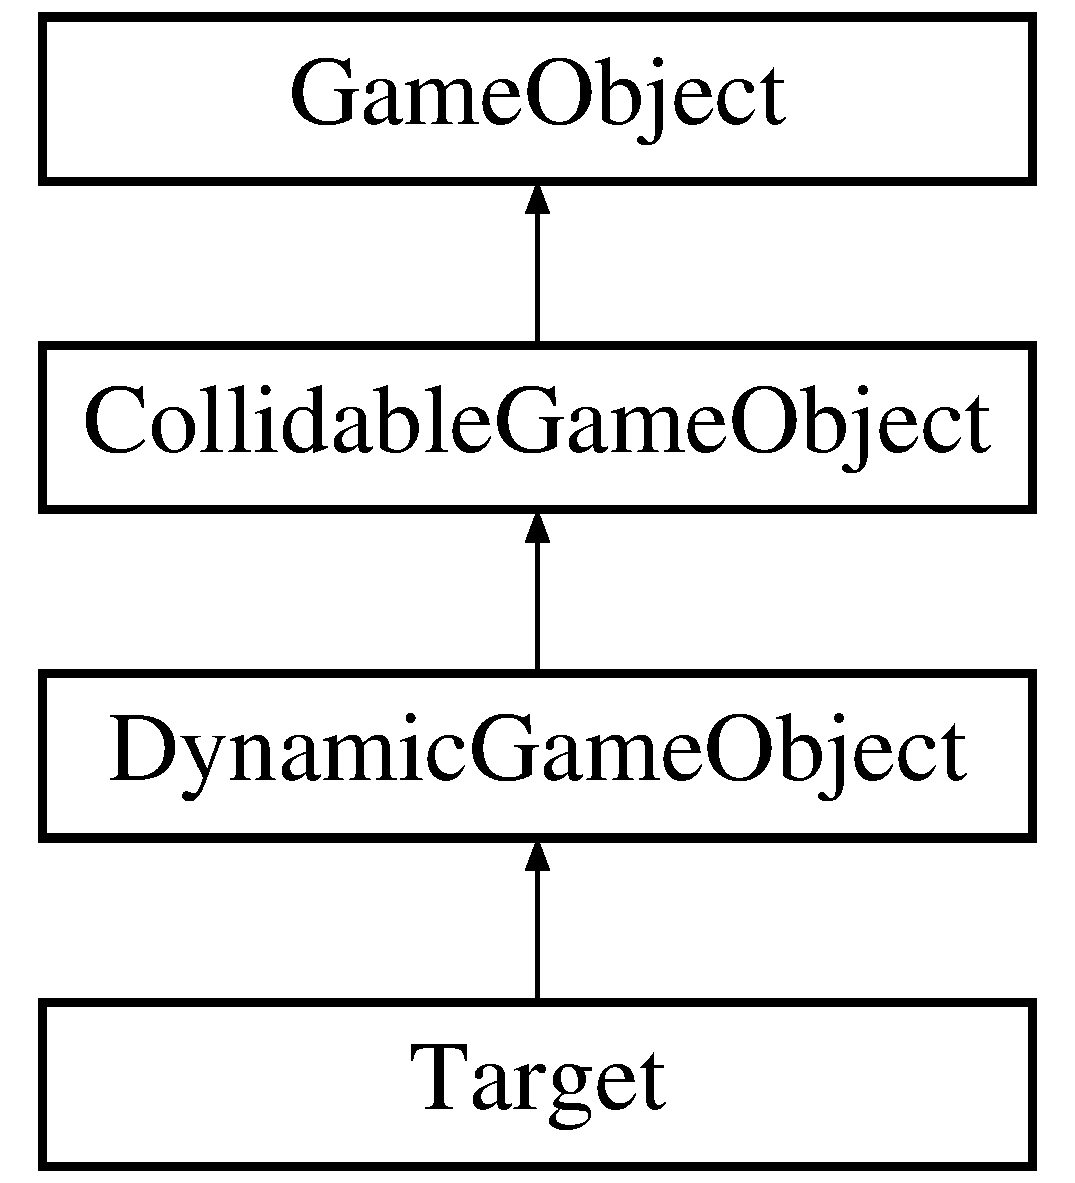
\includegraphics[height=4.000000cm]{class_target}
\end{center}
\end{figure}
\subsection*{Public Member Functions}
\begin{DoxyCompactItemize}
\item 
\hyperlink{class_target_ac423f1beea52507028b21180c3eadfd8}{Target} (\hyperlink{class_vector3}{Vector3} pos)
\item 
void \hyperlink{class_target_aca691803b6bb7185adc521d63cdd7835}{init} () override
\item 
void \hyperlink{class_target_a5f3b2dc70e8065e53199ab3244059ba7}{update} (int \hyperlink{_game_manager_8h_afea6a95c7a1c119b7106a4c735eb259d}{delta\+Time}) final
\item 
void \hyperlink{class_target_a03e4fae56bd104dadf5cec8247452c7e}{render} () final
\item 
void \hyperlink{class_target_a47eab7761cd91403698a23c65806cb28}{set\+Random\+Position} ()
\end{DoxyCompactItemize}
\subsection*{Public Attributes}
\begin{DoxyCompactItemize}
\item 
float \hyperlink{class_target_a55c8a14bee479115991505ae6dfff18a}{angle} = 0
\end{DoxyCompactItemize}
\subsection*{Additional Inherited Members}


\subsection{Constructor \& Destructor Documentation}
\mbox{\Hypertarget{class_target_ac423f1beea52507028b21180c3eadfd8}\label{class_target_ac423f1beea52507028b21180c3eadfd8}} 
\index{Target@{Target}!Target@{Target}}
\index{Target@{Target}!Target@{Target}}
\subsubsection{\texorpdfstring{Target()}{Target()}}
{\footnotesize\ttfamily Target\+::\+Target (\begin{DoxyParamCaption}\item[{\hyperlink{class_vector3}{Vector3}}]{pos }\end{DoxyParamCaption})\hspace{0.3cm}{\ttfamily [inline]}}



\subsection{Member Function Documentation}
\mbox{\Hypertarget{class_target_aca691803b6bb7185adc521d63cdd7835}\label{class_target_aca691803b6bb7185adc521d63cdd7835}} 
\index{Target@{Target}!init@{init}}
\index{init@{init}!Target@{Target}}
\subsubsection{\texorpdfstring{init()}{init()}}
{\footnotesize\ttfamily void Target\+::init (\begin{DoxyParamCaption}{ }\end{DoxyParamCaption})\hspace{0.3cm}{\ttfamily [inline]}, {\ttfamily [override]}, {\ttfamily [virtual]}}



Reimplemented from \hyperlink{class_game_object_aecb2c1b9f69715d854f7604d5d7978ec}{Game\+Object}.

\mbox{\Hypertarget{class_target_a03e4fae56bd104dadf5cec8247452c7e}\label{class_target_a03e4fae56bd104dadf5cec8247452c7e}} 
\index{Target@{Target}!render@{render}}
\index{render@{render}!Target@{Target}}
\subsubsection{\texorpdfstring{render()}{render()}}
{\footnotesize\ttfamily void Target\+::render (\begin{DoxyParamCaption}{ }\end{DoxyParamCaption})\hspace{0.3cm}{\ttfamily [inline]}, {\ttfamily [final]}, {\ttfamily [virtual]}}



Reimplemented from \hyperlink{class_game_object_a484efb66a7a27c101e84c11d9905d7a6}{Game\+Object}.

\mbox{\Hypertarget{class_target_a47eab7761cd91403698a23c65806cb28}\label{class_target_a47eab7761cd91403698a23c65806cb28}} 
\index{Target@{Target}!set\+Random\+Position@{set\+Random\+Position}}
\index{set\+Random\+Position@{set\+Random\+Position}!Target@{Target}}
\subsubsection{\texorpdfstring{set\+Random\+Position()}{setRandomPosition()}}
{\footnotesize\ttfamily void Target\+::set\+Random\+Position (\begin{DoxyParamCaption}{ }\end{DoxyParamCaption})\hspace{0.3cm}{\ttfamily [inline]}}

\mbox{\Hypertarget{class_target_a5f3b2dc70e8065e53199ab3244059ba7}\label{class_target_a5f3b2dc70e8065e53199ab3244059ba7}} 
\index{Target@{Target}!update@{update}}
\index{update@{update}!Target@{Target}}
\subsubsection{\texorpdfstring{update()}{update()}}
{\footnotesize\ttfamily void Target\+::update (\begin{DoxyParamCaption}\item[{int}]{delta\+Time }\end{DoxyParamCaption})\hspace{0.3cm}{\ttfamily [inline]}, {\ttfamily [final]}, {\ttfamily [virtual]}}



Reimplemented from \hyperlink{class_dynamic_game_object_aaa505b57d131bbbce44d500ec2ca0e83}{Dynamic\+Game\+Object}.



\subsection{Member Data Documentation}
\mbox{\Hypertarget{class_target_a55c8a14bee479115991505ae6dfff18a}\label{class_target_a55c8a14bee479115991505ae6dfff18a}} 
\index{Target@{Target}!angle@{angle}}
\index{angle@{angle}!Target@{Target}}
\subsubsection{\texorpdfstring{angle}{angle}}
{\footnotesize\ttfamily float Target\+::angle = 0}



The documentation for this class was generated from the following file\+:\begin{DoxyCompactItemize}
\item 
/\+Users/matya/\+A\+V\+T7/src/objects/\hyperlink{_target_8h}{Target.\+h}\end{DoxyCompactItemize}

\hypertarget{class_test_cube_collision}{}\section{Test\+Cube\+Collision Class Reference}
\label{class_test_cube_collision}\index{Test\+Cube\+Collision@{Test\+Cube\+Collision}}


{\ttfamily \#include $<$Test\+Cube\+Collision.\+h$>$}

Inheritance diagram for Test\+Cube\+Collision\+:\begin{figure}[H]
\begin{center}
\leavevmode
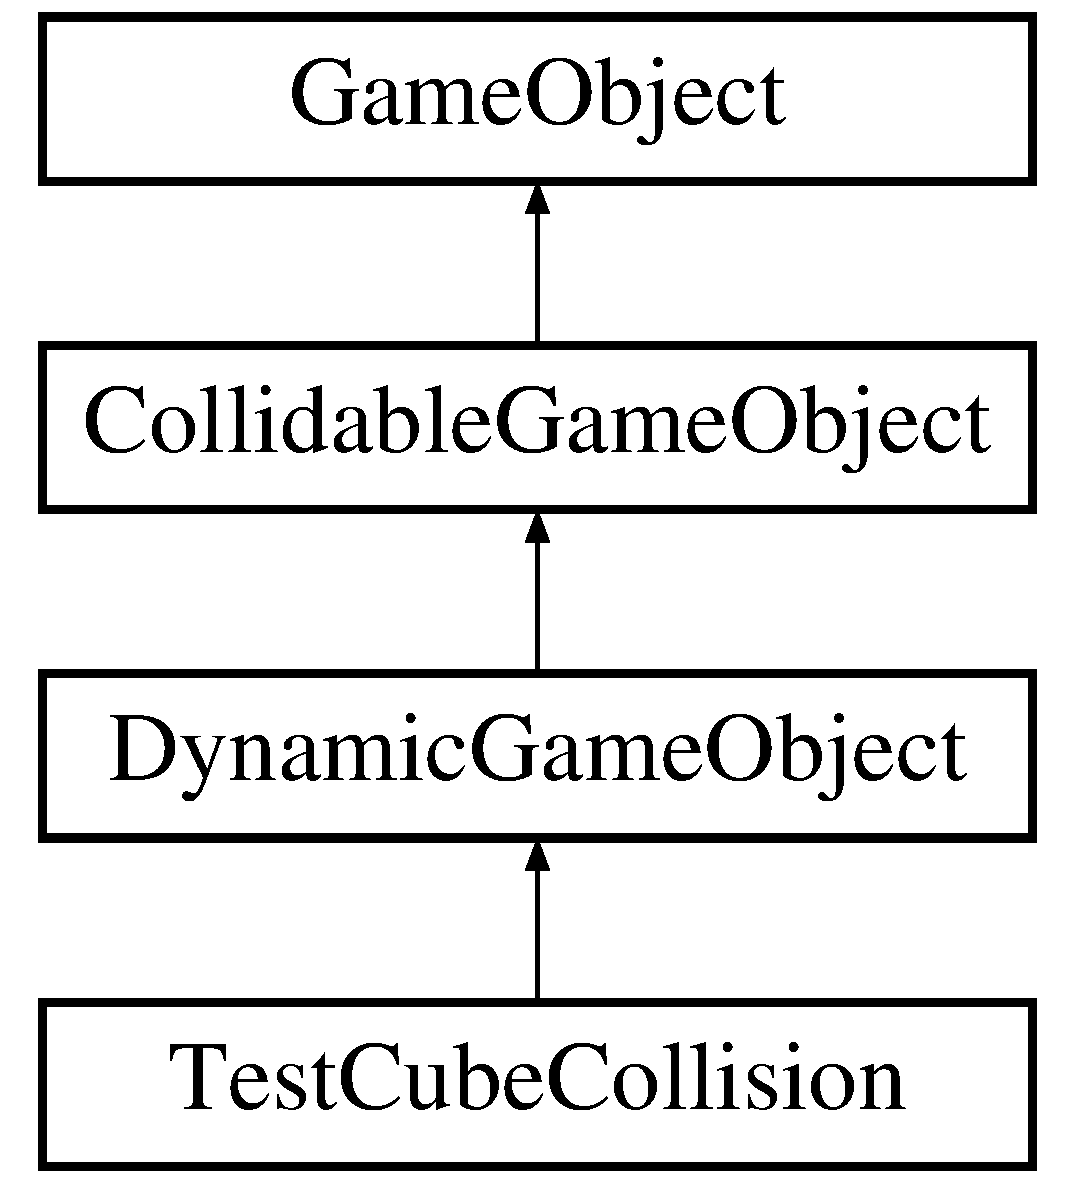
\includegraphics[height=4.000000cm]{class_test_cube_collision}
\end{center}
\end{figure}
\subsection*{Public Member Functions}
\begin{DoxyCompactItemize}
\item 
\hyperlink{class_test_cube_collision_a512c666b3899713b54b096e3e5ab5e58}{Test\+Cube\+Collision} (\hyperlink{class_vector3}{Vector3} pos, \hyperlink{class_vector3}{Vector3} \hyperlink{class_dynamic_game_object_a54cb8a3a5fe8314cd5751f223b2b49ae}{speed}, float tscale, \hyperlink{_game_object_8h_a57678b60d65afb213d04a6b090c64a08}{Game\+Object\+Type} type=T\+E\+ST, \hyperlink{class_vector3}{Vector3} min=\hyperlink{class_vector3}{Vector3}(0, 0, 0), \hyperlink{class_vector3}{Vector3} max=\hyperlink{class_vector3}{Vector3}(1, 1, 1))
\item 
virtual void \hyperlink{class_test_cube_collision_a796cf89af42a38b44956f753e14637b2}{respawn} ()
\item 
void \hyperlink{class_test_cube_collision_a22fade1ca48a2cd49dd4ca6cbc93821b}{init} () override
\item 
void \hyperlink{class_test_cube_collision_ae528ac632377372d93964c938748fddf}{update} (int \hyperlink{_game_manager_8h_afea6a95c7a1c119b7106a4c735eb259d}{delta\+Time}) final
\item 
void \hyperlink{class_test_cube_collision_ae5cd1052745d6acf9cbb2a6bde8b757a}{render} () override
\item 
bool \hyperlink{class_test_cube_collision_a94a32ad4ffd215b7c16efa866eb31ef2}{is\+Inside} (const \hyperlink{class_game_object}{Game\+Object} $\ast$other) const
\end{DoxyCompactItemize}
\subsection*{Public Attributes}
\begin{DoxyCompactItemize}
\item 
float \hyperlink{class_test_cube_collision_a3cd9b6464419d2c5a26bfc42d120819c}{mscale} = 0.\+0f
\end{DoxyCompactItemize}
\subsection*{Additional Inherited Members}


\subsection{Constructor \& Destructor Documentation}
\mbox{\Hypertarget{class_test_cube_collision_a512c666b3899713b54b096e3e5ab5e58}\label{class_test_cube_collision_a512c666b3899713b54b096e3e5ab5e58}} 
\index{Test\+Cube\+Collision@{Test\+Cube\+Collision}!Test\+Cube\+Collision@{Test\+Cube\+Collision}}
\index{Test\+Cube\+Collision@{Test\+Cube\+Collision}!Test\+Cube\+Collision@{Test\+Cube\+Collision}}
\subsubsection{\texorpdfstring{Test\+Cube\+Collision()}{TestCubeCollision()}}
{\footnotesize\ttfamily Test\+Cube\+Collision\+::\+Test\+Cube\+Collision (\begin{DoxyParamCaption}\item[{\hyperlink{class_vector3}{Vector3}}]{pos,  }\item[{\hyperlink{class_vector3}{Vector3}}]{speed,  }\item[{float}]{tscale,  }\item[{\hyperlink{_game_object_8h_a57678b60d65afb213d04a6b090c64a08}{Game\+Object\+Type}}]{type = {\ttfamily TEST},  }\item[{\hyperlink{class_vector3}{Vector3}}]{min = {\ttfamily \hyperlink{class_vector3}{Vector3}(0,~0,~0)},  }\item[{\hyperlink{class_vector3}{Vector3}}]{max = {\ttfamily \hyperlink{class_vector3}{Vector3}(1,~1,~1)} }\end{DoxyParamCaption})\hspace{0.3cm}{\ttfamily [inline]}}



\subsection{Member Function Documentation}
\mbox{\Hypertarget{class_test_cube_collision_a22fade1ca48a2cd49dd4ca6cbc93821b}\label{class_test_cube_collision_a22fade1ca48a2cd49dd4ca6cbc93821b}} 
\index{Test\+Cube\+Collision@{Test\+Cube\+Collision}!init@{init}}
\index{init@{init}!Test\+Cube\+Collision@{Test\+Cube\+Collision}}
\subsubsection{\texorpdfstring{init()}{init()}}
{\footnotesize\ttfamily void Test\+Cube\+Collision\+::init (\begin{DoxyParamCaption}{ }\end{DoxyParamCaption})\hspace{0.3cm}{\ttfamily [inline]}, {\ttfamily [override]}, {\ttfamily [virtual]}}



Reimplemented from \hyperlink{class_game_object_aecb2c1b9f69715d854f7604d5d7978ec}{Game\+Object}.

\mbox{\Hypertarget{class_test_cube_collision_a94a32ad4ffd215b7c16efa866eb31ef2}\label{class_test_cube_collision_a94a32ad4ffd215b7c16efa866eb31ef2}} 
\index{Test\+Cube\+Collision@{Test\+Cube\+Collision}!is\+Inside@{is\+Inside}}
\index{is\+Inside@{is\+Inside}!Test\+Cube\+Collision@{Test\+Cube\+Collision}}
\subsubsection{\texorpdfstring{is\+Inside()}{isInside()}}
{\footnotesize\ttfamily bool Test\+Cube\+Collision\+::is\+Inside (\begin{DoxyParamCaption}\item[{const \hyperlink{class_game_object}{Game\+Object} $\ast$}]{other }\end{DoxyParamCaption}) const\hspace{0.3cm}{\ttfamily [inline]}}

\mbox{\Hypertarget{class_test_cube_collision_ae5cd1052745d6acf9cbb2a6bde8b757a}\label{class_test_cube_collision_ae5cd1052745d6acf9cbb2a6bde8b757a}} 
\index{Test\+Cube\+Collision@{Test\+Cube\+Collision}!render@{render}}
\index{render@{render}!Test\+Cube\+Collision@{Test\+Cube\+Collision}}
\subsubsection{\texorpdfstring{render()}{render()}}
{\footnotesize\ttfamily void Test\+Cube\+Collision\+::render (\begin{DoxyParamCaption}{ }\end{DoxyParamCaption})\hspace{0.3cm}{\ttfamily [inline]}, {\ttfamily [override]}, {\ttfamily [virtual]}}



Reimplemented from \hyperlink{class_game_object_a484efb66a7a27c101e84c11d9905d7a6}{Game\+Object}.

\mbox{\Hypertarget{class_test_cube_collision_a796cf89af42a38b44956f753e14637b2}\label{class_test_cube_collision_a796cf89af42a38b44956f753e14637b2}} 
\index{Test\+Cube\+Collision@{Test\+Cube\+Collision}!respawn@{respawn}}
\index{respawn@{respawn}!Test\+Cube\+Collision@{Test\+Cube\+Collision}}
\subsubsection{\texorpdfstring{respawn()}{respawn()}}
{\footnotesize\ttfamily virtual void Test\+Cube\+Collision\+::respawn (\begin{DoxyParamCaption}{ }\end{DoxyParamCaption})\hspace{0.3cm}{\ttfamily [inline]}, {\ttfamily [virtual]}}

\mbox{\Hypertarget{class_test_cube_collision_ae528ac632377372d93964c938748fddf}\label{class_test_cube_collision_ae528ac632377372d93964c938748fddf}} 
\index{Test\+Cube\+Collision@{Test\+Cube\+Collision}!update@{update}}
\index{update@{update}!Test\+Cube\+Collision@{Test\+Cube\+Collision}}
\subsubsection{\texorpdfstring{update()}{update()}}
{\footnotesize\ttfamily void Test\+Cube\+Collision\+::update (\begin{DoxyParamCaption}\item[{int}]{delta\+Time }\end{DoxyParamCaption})\hspace{0.3cm}{\ttfamily [inline]}, {\ttfamily [final]}, {\ttfamily [virtual]}}



Reimplemented from \hyperlink{class_dynamic_game_object_aaa505b57d131bbbce44d500ec2ca0e83}{Dynamic\+Game\+Object}.



\subsection{Member Data Documentation}
\mbox{\Hypertarget{class_test_cube_collision_a3cd9b6464419d2c5a26bfc42d120819c}\label{class_test_cube_collision_a3cd9b6464419d2c5a26bfc42d120819c}} 
\index{Test\+Cube\+Collision@{Test\+Cube\+Collision}!mscale@{mscale}}
\index{mscale@{mscale}!Test\+Cube\+Collision@{Test\+Cube\+Collision}}
\subsubsection{\texorpdfstring{mscale}{mscale}}
{\footnotesize\ttfamily float Test\+Cube\+Collision\+::mscale = 0.\+0f}



The documentation for this class was generated from the following file\+:\begin{DoxyCompactItemize}
\item 
/\+Users/matya/\+A\+V\+T7/src/objects/\hyperlink{_test_cube_collision_8h}{Test\+Cube\+Collision.\+h}\end{DoxyCompactItemize}

\hypertarget{class_turtle}{}\section{Turtle Class Reference}
\label{class_turtle}\index{Turtle@{Turtle}}


{\ttfamily \#include $<$Turtle.\+h$>$}

Inheritance diagram for Turtle\+:\begin{figure}[H]
\begin{center}
\leavevmode
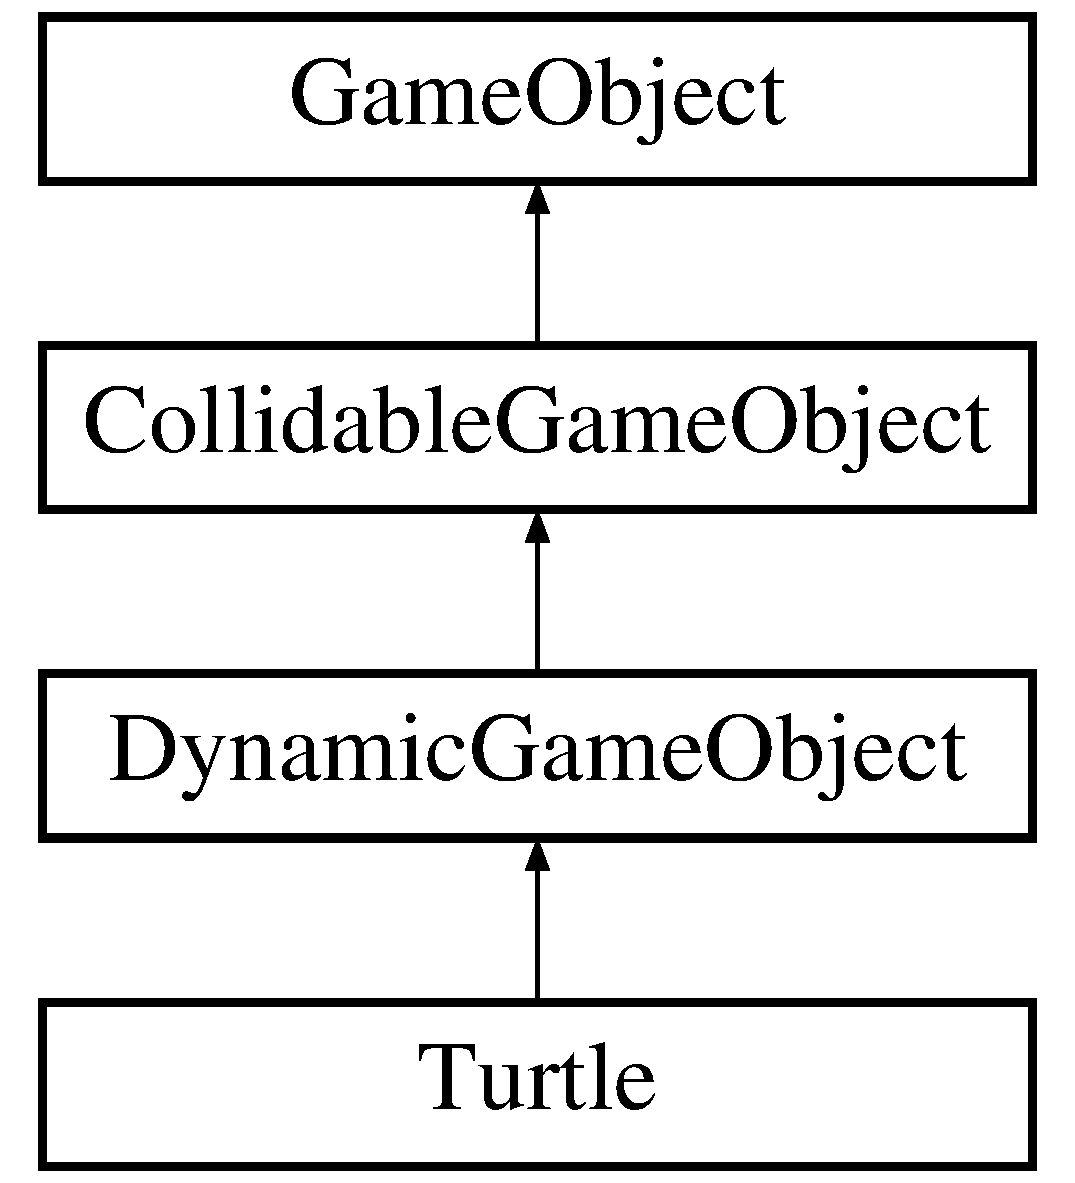
\includegraphics[height=4.000000cm]{class_turtle}
\end{center}
\end{figure}
\subsection*{Public Member Functions}
\begin{DoxyCompactItemize}
\item 
\hyperlink{class_turtle_a970240e0b41cea58ef93f8f0d3e17fd4}{Turtle} (\hyperlink{class_vector3}{Vector3} pos, \hyperlink{class_vector3}{Vector3} \hyperlink{class_dynamic_game_object_a54cb8a3a5fe8314cd5751f223b2b49ae}{speed})
\item 
void \hyperlink{class_turtle_a6ba4b31af71ea52e0e885a3e3beb783c}{init} () override
\item 
void \hyperlink{class_turtle_a697924198490c52307fdb006f1df7456}{render} () override
\item 
void \hyperlink{class_turtle_a6c70cb2158f173b82df6620905ad435c}{respawn} ()
\item 
void \hyperlink{class_turtle_a6d62e3f4e21f5ce3ffb4e7e2a8a9da1b}{update} (int \hyperlink{_game_manager_8h_afea6a95c7a1c119b7106a4c735eb259d}{delta\+Time}) override
\end{DoxyCompactItemize}
\subsection*{Public Attributes}
\begin{DoxyCompactItemize}
\item 
\hyperlink{class_vector3}{Vector3} \hyperlink{class_turtle_a9052d3e0b90f7334d5fb3ac37617b3a6}{init\+Pos}
\item 
\hyperlink{class_vector3}{Vector3} \hyperlink{class_turtle_a085cc226004058c86277dfe21a2dc077}{init\+Speed}
\item 
float \hyperlink{class_turtle_a827a4dc9095185fd3e7fd1a56e6e3587}{random\+Time\+Offset} = 0.\+0f
\item 
const float \hyperlink{class_turtle_ab854ea2525dee2b36f2eba8f16573287}{wave\+Time} = 1000.\+0f
\item 
G\+Lint \hyperlink{class_turtle_a786de5c643f4bb563bbf851da057a85b}{prev\+Time} = 1
\item 
bool \hyperlink{class_turtle_a4a81d2f3cef8a9d8556f05b6356d0fd2}{is\+Under\+Water} = false
\item 
float \hyperlink{class_turtle_a4e52ca74d8dff20d4e1aa16a1774dea4}{pos\+Turtle\+Body\+Water} = 0.\+2f
\end{DoxyCompactItemize}
\subsection*{Additional Inherited Members}


\subsection{Constructor \& Destructor Documentation}
\mbox{\Hypertarget{class_turtle_a970240e0b41cea58ef93f8f0d3e17fd4}\label{class_turtle_a970240e0b41cea58ef93f8f0d3e17fd4}} 
\index{Turtle@{Turtle}!Turtle@{Turtle}}
\index{Turtle@{Turtle}!Turtle@{Turtle}}
\subsubsection{\texorpdfstring{Turtle()}{Turtle()}}
{\footnotesize\ttfamily Turtle\+::\+Turtle (\begin{DoxyParamCaption}\item[{\hyperlink{class_vector3}{Vector3}}]{pos,  }\item[{\hyperlink{class_vector3}{Vector3}}]{speed }\end{DoxyParamCaption})\hspace{0.3cm}{\ttfamily [inline]}}



\subsection{Member Function Documentation}
\mbox{\Hypertarget{class_turtle_a6ba4b31af71ea52e0e885a3e3beb783c}\label{class_turtle_a6ba4b31af71ea52e0e885a3e3beb783c}} 
\index{Turtle@{Turtle}!init@{init}}
\index{init@{init}!Turtle@{Turtle}}
\subsubsection{\texorpdfstring{init()}{init()}}
{\footnotesize\ttfamily void Turtle\+::init (\begin{DoxyParamCaption}{ }\end{DoxyParamCaption})\hspace{0.3cm}{\ttfamily [inline]}, {\ttfamily [override]}, {\ttfamily [virtual]}}



Reimplemented from \hyperlink{class_game_object_aecb2c1b9f69715d854f7604d5d7978ec}{Game\+Object}.

\mbox{\Hypertarget{class_turtle_a697924198490c52307fdb006f1df7456}\label{class_turtle_a697924198490c52307fdb006f1df7456}} 
\index{Turtle@{Turtle}!render@{render}}
\index{render@{render}!Turtle@{Turtle}}
\subsubsection{\texorpdfstring{render()}{render()}}
{\footnotesize\ttfamily void Turtle\+::render (\begin{DoxyParamCaption}{ }\end{DoxyParamCaption})\hspace{0.3cm}{\ttfamily [inline]}, {\ttfamily [override]}, {\ttfamily [virtual]}}



Reimplemented from \hyperlink{class_game_object_a484efb66a7a27c101e84c11d9905d7a6}{Game\+Object}.

\mbox{\Hypertarget{class_turtle_a6c70cb2158f173b82df6620905ad435c}\label{class_turtle_a6c70cb2158f173b82df6620905ad435c}} 
\index{Turtle@{Turtle}!respawn@{respawn}}
\index{respawn@{respawn}!Turtle@{Turtle}}
\subsubsection{\texorpdfstring{respawn()}{respawn()}}
{\footnotesize\ttfamily void Turtle\+::respawn (\begin{DoxyParamCaption}{ }\end{DoxyParamCaption})\hspace{0.3cm}{\ttfamily [inline]}}

\mbox{\Hypertarget{class_turtle_a6d62e3f4e21f5ce3ffb4e7e2a8a9da1b}\label{class_turtle_a6d62e3f4e21f5ce3ffb4e7e2a8a9da1b}} 
\index{Turtle@{Turtle}!update@{update}}
\index{update@{update}!Turtle@{Turtle}}
\subsubsection{\texorpdfstring{update()}{update()}}
{\footnotesize\ttfamily void Turtle\+::update (\begin{DoxyParamCaption}\item[{int}]{delta\+Time }\end{DoxyParamCaption})\hspace{0.3cm}{\ttfamily [inline]}, {\ttfamily [override]}, {\ttfamily [virtual]}}



Reimplemented from \hyperlink{class_dynamic_game_object_aaa505b57d131bbbce44d500ec2ca0e83}{Dynamic\+Game\+Object}.



\subsection{Member Data Documentation}
\mbox{\Hypertarget{class_turtle_a9052d3e0b90f7334d5fb3ac37617b3a6}\label{class_turtle_a9052d3e0b90f7334d5fb3ac37617b3a6}} 
\index{Turtle@{Turtle}!init\+Pos@{init\+Pos}}
\index{init\+Pos@{init\+Pos}!Turtle@{Turtle}}
\subsubsection{\texorpdfstring{init\+Pos}{initPos}}
{\footnotesize\ttfamily \hyperlink{class_vector3}{Vector3} Turtle\+::init\+Pos}

\mbox{\Hypertarget{class_turtle_a085cc226004058c86277dfe21a2dc077}\label{class_turtle_a085cc226004058c86277dfe21a2dc077}} 
\index{Turtle@{Turtle}!init\+Speed@{init\+Speed}}
\index{init\+Speed@{init\+Speed}!Turtle@{Turtle}}
\subsubsection{\texorpdfstring{init\+Speed}{initSpeed}}
{\footnotesize\ttfamily \hyperlink{class_vector3}{Vector3} Turtle\+::init\+Speed}

\mbox{\Hypertarget{class_turtle_a4a81d2f3cef8a9d8556f05b6356d0fd2}\label{class_turtle_a4a81d2f3cef8a9d8556f05b6356d0fd2}} 
\index{Turtle@{Turtle}!is\+Under\+Water@{is\+Under\+Water}}
\index{is\+Under\+Water@{is\+Under\+Water}!Turtle@{Turtle}}
\subsubsection{\texorpdfstring{is\+Under\+Water}{isUnderWater}}
{\footnotesize\ttfamily bool Turtle\+::is\+Under\+Water = false}

\mbox{\Hypertarget{class_turtle_a4e52ca74d8dff20d4e1aa16a1774dea4}\label{class_turtle_a4e52ca74d8dff20d4e1aa16a1774dea4}} 
\index{Turtle@{Turtle}!pos\+Turtle\+Body\+Water@{pos\+Turtle\+Body\+Water}}
\index{pos\+Turtle\+Body\+Water@{pos\+Turtle\+Body\+Water}!Turtle@{Turtle}}
\subsubsection{\texorpdfstring{pos\+Turtle\+Body\+Water}{posTurtleBodyWater}}
{\footnotesize\ttfamily float Turtle\+::pos\+Turtle\+Body\+Water = 0.\+2f}

\mbox{\Hypertarget{class_turtle_a786de5c643f4bb563bbf851da057a85b}\label{class_turtle_a786de5c643f4bb563bbf851da057a85b}} 
\index{Turtle@{Turtle}!prev\+Time@{prev\+Time}}
\index{prev\+Time@{prev\+Time}!Turtle@{Turtle}}
\subsubsection{\texorpdfstring{prev\+Time}{prevTime}}
{\footnotesize\ttfamily G\+Lint Turtle\+::prev\+Time = 1}

\mbox{\Hypertarget{class_turtle_a827a4dc9095185fd3e7fd1a56e6e3587}\label{class_turtle_a827a4dc9095185fd3e7fd1a56e6e3587}} 
\index{Turtle@{Turtle}!random\+Time\+Offset@{random\+Time\+Offset}}
\index{random\+Time\+Offset@{random\+Time\+Offset}!Turtle@{Turtle}}
\subsubsection{\texorpdfstring{random\+Time\+Offset}{randomTimeOffset}}
{\footnotesize\ttfamily float Turtle\+::random\+Time\+Offset = 0.\+0f}

\mbox{\Hypertarget{class_turtle_ab854ea2525dee2b36f2eba8f16573287}\label{class_turtle_ab854ea2525dee2b36f2eba8f16573287}} 
\index{Turtle@{Turtle}!wave\+Time@{wave\+Time}}
\index{wave\+Time@{wave\+Time}!Turtle@{Turtle}}
\subsubsection{\texorpdfstring{wave\+Time}{waveTime}}
{\footnotesize\ttfamily const float Turtle\+::wave\+Time = 1000.\+0f}



The documentation for this class was generated from the following file\+:\begin{DoxyCompactItemize}
\item 
/\+Users/matya/\+A\+V\+T7/src/objects/\hyperlink{_turtle_8h}{Turtle.\+h}\end{DoxyCompactItemize}

\hypertarget{class_v_s_shader_lib_1_1_uniform_block}{}\section{V\+S\+Shader\+Lib\+:\+:Uniform\+Block Class Reference}
\label{class_v_s_shader_lib_1_1_uniform_block}\index{V\+S\+Shader\+Lib\+::\+Uniform\+Block@{V\+S\+Shader\+Lib\+::\+Uniform\+Block}}


stores information for a block and its uniforms  




{\ttfamily \#include $<$vs\+Shader\+Lib.\+h$>$}

\subsection*{Public Attributes}
\begin{DoxyCompactItemize}
\item 
int \hyperlink{class_v_s_shader_lib_1_1_uniform_block_a71d5bc23b4f834a62391daf8f655b97d}{size}
\begin{DoxyCompactList}\small\item\em size of the uniform block \end{DoxyCompactList}\item 
G\+Luint \hyperlink{class_v_s_shader_lib_1_1_uniform_block_a61db2ec3b1ac47ac0198f99b28ea8bfd}{buffer}
\begin{DoxyCompactList}\small\item\em buffer bound to the index point \end{DoxyCompactList}\item 
G\+Luint \hyperlink{class_v_s_shader_lib_1_1_uniform_block_a1694ff57ebbee6c2cc3ce513cce84431}{binding\+Index}
\begin{DoxyCompactList}\small\item\em binding index \end{DoxyCompactList}\item 
std\+::map$<$ std\+::string, \hyperlink{class_v_s_shader_lib_a0543003357c93b57bfe99a9aa3e0898d}{my\+Block\+Uniform} $>$ \hyperlink{class_v_s_shader_lib_1_1_uniform_block_a94df01b8bf010f83a750d9807139c43f}{uniform\+Offsets}
\begin{DoxyCompactList}\small\item\em uniforms information \end{DoxyCompactList}\end{DoxyCompactItemize}


\subsection{Detailed Description}
stores information for a block and its uniforms 

\subsection{Member Data Documentation}
\mbox{\Hypertarget{class_v_s_shader_lib_1_1_uniform_block_a1694ff57ebbee6c2cc3ce513cce84431}\label{class_v_s_shader_lib_1_1_uniform_block_a1694ff57ebbee6c2cc3ce513cce84431}} 
\index{V\+S\+Shader\+Lib\+::\+Uniform\+Block@{V\+S\+Shader\+Lib\+::\+Uniform\+Block}!binding\+Index@{binding\+Index}}
\index{binding\+Index@{binding\+Index}!V\+S\+Shader\+Lib\+::\+Uniform\+Block@{V\+S\+Shader\+Lib\+::\+Uniform\+Block}}
\subsubsection{\texorpdfstring{binding\+Index}{bindingIndex}}
{\footnotesize\ttfamily G\+Luint V\+S\+Shader\+Lib\+::\+Uniform\+Block\+::binding\+Index}



binding index 

\mbox{\Hypertarget{class_v_s_shader_lib_1_1_uniform_block_a61db2ec3b1ac47ac0198f99b28ea8bfd}\label{class_v_s_shader_lib_1_1_uniform_block_a61db2ec3b1ac47ac0198f99b28ea8bfd}} 
\index{V\+S\+Shader\+Lib\+::\+Uniform\+Block@{V\+S\+Shader\+Lib\+::\+Uniform\+Block}!buffer@{buffer}}
\index{buffer@{buffer}!V\+S\+Shader\+Lib\+::\+Uniform\+Block@{V\+S\+Shader\+Lib\+::\+Uniform\+Block}}
\subsubsection{\texorpdfstring{buffer}{buffer}}
{\footnotesize\ttfamily G\+Luint V\+S\+Shader\+Lib\+::\+Uniform\+Block\+::buffer}



buffer bound to the index point 

\mbox{\Hypertarget{class_v_s_shader_lib_1_1_uniform_block_a71d5bc23b4f834a62391daf8f655b97d}\label{class_v_s_shader_lib_1_1_uniform_block_a71d5bc23b4f834a62391daf8f655b97d}} 
\index{V\+S\+Shader\+Lib\+::\+Uniform\+Block@{V\+S\+Shader\+Lib\+::\+Uniform\+Block}!size@{size}}
\index{size@{size}!V\+S\+Shader\+Lib\+::\+Uniform\+Block@{V\+S\+Shader\+Lib\+::\+Uniform\+Block}}
\subsubsection{\texorpdfstring{size}{size}}
{\footnotesize\ttfamily int V\+S\+Shader\+Lib\+::\+Uniform\+Block\+::size}



size of the uniform block 

\mbox{\Hypertarget{class_v_s_shader_lib_1_1_uniform_block_a94df01b8bf010f83a750d9807139c43f}\label{class_v_s_shader_lib_1_1_uniform_block_a94df01b8bf010f83a750d9807139c43f}} 
\index{V\+S\+Shader\+Lib\+::\+Uniform\+Block@{V\+S\+Shader\+Lib\+::\+Uniform\+Block}!uniform\+Offsets@{uniform\+Offsets}}
\index{uniform\+Offsets@{uniform\+Offsets}!V\+S\+Shader\+Lib\+::\+Uniform\+Block@{V\+S\+Shader\+Lib\+::\+Uniform\+Block}}
\subsubsection{\texorpdfstring{uniform\+Offsets}{uniformOffsets}}
{\footnotesize\ttfamily std\+::map$<$std\+::string, \hyperlink{class_v_s_shader_lib_a0543003357c93b57bfe99a9aa3e0898d}{my\+Block\+Uniform} $>$ V\+S\+Shader\+Lib\+::\+Uniform\+Block\+::uniform\+Offsets}



uniforms information 



The documentation for this class was generated from the following file\+:\begin{DoxyCompactItemize}
\item 
/\+Users/matya/\+A\+V\+T7/src/libs/\hyperlink{vs_shader_lib_8h}{vs\+Shader\+Lib.\+h}\end{DoxyCompactItemize}

\hypertarget{struct_v_s_shader_lib_1_1uniforms}{}\section{V\+S\+Shader\+Lib\+:\+:uniforms Struct Reference}
\label{struct_v_s_shader_lib_1_1uniforms}\index{V\+S\+Shader\+Lib\+::uniforms@{V\+S\+Shader\+Lib\+::uniforms}}


stores information for uniforms  




{\ttfamily \#include $<$vs\+Shader\+Lib.\+h$>$}

\subsection*{Public Attributes}
\begin{DoxyCompactItemize}
\item 
G\+Lenum \hyperlink{struct_v_s_shader_lib_1_1uniforms_a24f7a9f89bd519b943015bc30ca7501b}{type}
\item 
G\+Luint \hyperlink{struct_v_s_shader_lib_1_1uniforms_a223d7fcee1d156215f76d9f2181e0033}{location}
\item 
G\+Luint \hyperlink{struct_v_s_shader_lib_1_1uniforms_afcc7514fb51e3109902164a9f5dd9d59}{size}
\item 
G\+Luint \hyperlink{struct_v_s_shader_lib_1_1uniforms_afa69bd45798a24073958bf99a9cacdc8}{stride}
\end{DoxyCompactItemize}


\subsection{Detailed Description}
stores information for uniforms 

\subsection{Member Data Documentation}
\mbox{\Hypertarget{struct_v_s_shader_lib_1_1uniforms_a223d7fcee1d156215f76d9f2181e0033}\label{struct_v_s_shader_lib_1_1uniforms_a223d7fcee1d156215f76d9f2181e0033}} 
\index{V\+S\+Shader\+Lib\+::uniforms@{V\+S\+Shader\+Lib\+::uniforms}!location@{location}}
\index{location@{location}!V\+S\+Shader\+Lib\+::uniforms@{V\+S\+Shader\+Lib\+::uniforms}}
\subsubsection{\texorpdfstring{location}{location}}
{\footnotesize\ttfamily G\+Luint V\+S\+Shader\+Lib\+::uniforms\+::location}

\mbox{\Hypertarget{struct_v_s_shader_lib_1_1uniforms_afcc7514fb51e3109902164a9f5dd9d59}\label{struct_v_s_shader_lib_1_1uniforms_afcc7514fb51e3109902164a9f5dd9d59}} 
\index{V\+S\+Shader\+Lib\+::uniforms@{V\+S\+Shader\+Lib\+::uniforms}!size@{size}}
\index{size@{size}!V\+S\+Shader\+Lib\+::uniforms@{V\+S\+Shader\+Lib\+::uniforms}}
\subsubsection{\texorpdfstring{size}{size}}
{\footnotesize\ttfamily G\+Luint V\+S\+Shader\+Lib\+::uniforms\+::size}

\mbox{\Hypertarget{struct_v_s_shader_lib_1_1uniforms_afa69bd45798a24073958bf99a9cacdc8}\label{struct_v_s_shader_lib_1_1uniforms_afa69bd45798a24073958bf99a9cacdc8}} 
\index{V\+S\+Shader\+Lib\+::uniforms@{V\+S\+Shader\+Lib\+::uniforms}!stride@{stride}}
\index{stride@{stride}!V\+S\+Shader\+Lib\+::uniforms@{V\+S\+Shader\+Lib\+::uniforms}}
\subsubsection{\texorpdfstring{stride}{stride}}
{\footnotesize\ttfamily G\+Luint V\+S\+Shader\+Lib\+::uniforms\+::stride}

\mbox{\Hypertarget{struct_v_s_shader_lib_1_1uniforms_a24f7a9f89bd519b943015bc30ca7501b}\label{struct_v_s_shader_lib_1_1uniforms_a24f7a9f89bd519b943015bc30ca7501b}} 
\index{V\+S\+Shader\+Lib\+::uniforms@{V\+S\+Shader\+Lib\+::uniforms}!type@{type}}
\index{type@{type}!V\+S\+Shader\+Lib\+::uniforms@{V\+S\+Shader\+Lib\+::uniforms}}
\subsubsection{\texorpdfstring{type}{type}}
{\footnotesize\ttfamily G\+Lenum V\+S\+Shader\+Lib\+::uniforms\+::type}



The documentation for this struct was generated from the following file\+:\begin{DoxyCompactItemize}
\item 
/\+Users/matya/\+A\+V\+T7/src/libs/\hyperlink{vs_shader_lib_8h}{vs\+Shader\+Lib.\+h}\end{DoxyCompactItemize}

\hypertarget{class_vector3}{}\section{Vector3 Class Reference}
\label{class_vector3}\index{Vector3@{Vector3}}


{\ttfamily \#include $<$Vector3.\+h$>$}

\subsection*{Public Member Functions}
\begin{DoxyCompactItemize}
\item 
\hyperlink{class_vector3_a0e04c223104cd5f8089e8a34069e0d31}{Vector3} (float val=0)
\item 
\hyperlink{class_vector3_ad53e22b52babdb90d423601f72467590}{Vector3} (float \hyperlink{class_vector3_a7e2d3237b29a2f29d7b3d8b2934e35f2}{x}, float \hyperlink{class_vector3_a86eb35a9fa2d5a49e7fad66a35fa9c13}{y}, float \hyperlink{class_vector3_aa8c9461eb24bd2c364258078811a3e9d}{z})
\item 
bool \hyperlink{class_vector3_aea67111b0bc5b12c341145f84f3e2cff}{operator==} (const \hyperlink{class_vector3}{Vector3} \&vec) const
\item 
\hyperlink{class_vector3}{Vector3} \hyperlink{class_vector3_a87c9bc23295bebc6b36fd9b9c9abda67}{operator+} (const \hyperlink{class_vector3}{Vector3} \&vec) const
\item 
\hyperlink{class_vector3}{Vector3} \hyperlink{class_vector3_afb3734d29da79f12b1b02e0542433bd3}{operator-\/} (const \hyperlink{class_vector3}{Vector3} \&vec) const
\item 
\hyperlink{class_vector3}{Vector3} \hyperlink{class_vector3_ad572247e5bd9afab9d1639610f0b0ac6}{operator$\ast$} (float scalar) const
\item 
\hyperlink{class_vector3}{Vector3} \hyperlink{class_vector3_ad9ced662f4acf9c06de6655bd33ea683}{operator/} (float scalar) const
\item 
\hyperlink{class_vector3}{Vector3} \hyperlink{class_vector3_abf941de6e1724901c46d5e9e1448358f}{operator-\/} () const
\item 
bool \hyperlink{class_vector3_a4c506690133a1c5643734e23e7d69d5d}{operator$>$} (const \hyperlink{class_vector3}{Vector3} \&vec) const
\item 
void \hyperlink{class_vector3_a814c9ffea79062ce4d9ce902da1b6d05}{operator=} (const \hyperlink{class_vector3}{Vector3} \&vec)
\item 
float \hyperlink{class_vector3_a9dd2015e58d753dd4e3f1ba47eeaaf35}{distance} (const \hyperlink{class_vector3}{Vector3} \&vec) const
\end{DoxyCompactItemize}
\subsection*{Public Attributes}
\begin{DoxyCompactItemize}
\item 
float \hyperlink{class_vector3_a7e2d3237b29a2f29d7b3d8b2934e35f2}{x}
\item 
float \hyperlink{class_vector3_a86eb35a9fa2d5a49e7fad66a35fa9c13}{y}
\item 
float \hyperlink{class_vector3_aa8c9461eb24bd2c364258078811a3e9d}{z}
\end{DoxyCompactItemize}
\subsection*{Friends}
\begin{DoxyCompactItemize}
\item 
ostream \& \hyperlink{class_vector3_af8071adba02246ed84b6ac3e3f8d4737}{operator$<$$<$} (ostream \&os, const \hyperlink{class_vector3}{Vector3} \&vec)
\end{DoxyCompactItemize}


\subsection{Constructor \& Destructor Documentation}
\mbox{\Hypertarget{class_vector3_a0e04c223104cd5f8089e8a34069e0d31}\label{class_vector3_a0e04c223104cd5f8089e8a34069e0d31}} 
\index{Vector3@{Vector3}!Vector3@{Vector3}}
\index{Vector3@{Vector3}!Vector3@{Vector3}}
\subsubsection{\texorpdfstring{Vector3()}{Vector3()}\hspace{0.1cm}{\footnotesize\ttfamily [1/2]}}
{\footnotesize\ttfamily Vector3\+::\+Vector3 (\begin{DoxyParamCaption}\item[{float}]{val = {\ttfamily 0} }\end{DoxyParamCaption})\hspace{0.3cm}{\ttfamily [inline]}, {\ttfamily [explicit]}}

\mbox{\Hypertarget{class_vector3_ad53e22b52babdb90d423601f72467590}\label{class_vector3_ad53e22b52babdb90d423601f72467590}} 
\index{Vector3@{Vector3}!Vector3@{Vector3}}
\index{Vector3@{Vector3}!Vector3@{Vector3}}
\subsubsection{\texorpdfstring{Vector3()}{Vector3()}\hspace{0.1cm}{\footnotesize\ttfamily [2/2]}}
{\footnotesize\ttfamily Vector3\+::\+Vector3 (\begin{DoxyParamCaption}\item[{float}]{x,  }\item[{float}]{y,  }\item[{float}]{z }\end{DoxyParamCaption})\hspace{0.3cm}{\ttfamily [inline]}}



\subsection{Member Function Documentation}
\mbox{\Hypertarget{class_vector3_a9dd2015e58d753dd4e3f1ba47eeaaf35}\label{class_vector3_a9dd2015e58d753dd4e3f1ba47eeaaf35}} 
\index{Vector3@{Vector3}!distance@{distance}}
\index{distance@{distance}!Vector3@{Vector3}}
\subsubsection{\texorpdfstring{distance()}{distance()}}
{\footnotesize\ttfamily float Vector3\+::distance (\begin{DoxyParamCaption}\item[{const \hyperlink{class_vector3}{Vector3} \&}]{vec }\end{DoxyParamCaption}) const\hspace{0.3cm}{\ttfamily [inline]}}

\mbox{\Hypertarget{class_vector3_ad572247e5bd9afab9d1639610f0b0ac6}\label{class_vector3_ad572247e5bd9afab9d1639610f0b0ac6}} 
\index{Vector3@{Vector3}!operator$\ast$@{operator$\ast$}}
\index{operator$\ast$@{operator$\ast$}!Vector3@{Vector3}}
\subsubsection{\texorpdfstring{operator$\ast$()}{operator*()}}
{\footnotesize\ttfamily \hyperlink{class_vector3}{Vector3} Vector3\+::operator$\ast$ (\begin{DoxyParamCaption}\item[{float}]{scalar }\end{DoxyParamCaption}) const\hspace{0.3cm}{\ttfamily [inline]}}

\mbox{\Hypertarget{class_vector3_a87c9bc23295bebc6b36fd9b9c9abda67}\label{class_vector3_a87c9bc23295bebc6b36fd9b9c9abda67}} 
\index{Vector3@{Vector3}!operator+@{operator+}}
\index{operator+@{operator+}!Vector3@{Vector3}}
\subsubsection{\texorpdfstring{operator+()}{operator+()}}
{\footnotesize\ttfamily \hyperlink{class_vector3}{Vector3} Vector3\+::operator+ (\begin{DoxyParamCaption}\item[{const \hyperlink{class_vector3}{Vector3} \&}]{vec }\end{DoxyParamCaption}) const\hspace{0.3cm}{\ttfamily [inline]}}

\mbox{\Hypertarget{class_vector3_afb3734d29da79f12b1b02e0542433bd3}\label{class_vector3_afb3734d29da79f12b1b02e0542433bd3}} 
\index{Vector3@{Vector3}!operator-\/@{operator-\/}}
\index{operator-\/@{operator-\/}!Vector3@{Vector3}}
\subsubsection{\texorpdfstring{operator-\/()}{operator-()}\hspace{0.1cm}{\footnotesize\ttfamily [1/2]}}
{\footnotesize\ttfamily \hyperlink{class_vector3}{Vector3} Vector3\+::operator-\/ (\begin{DoxyParamCaption}\item[{const \hyperlink{class_vector3}{Vector3} \&}]{vec }\end{DoxyParamCaption}) const\hspace{0.3cm}{\ttfamily [inline]}}

\mbox{\Hypertarget{class_vector3_abf941de6e1724901c46d5e9e1448358f}\label{class_vector3_abf941de6e1724901c46d5e9e1448358f}} 
\index{Vector3@{Vector3}!operator-\/@{operator-\/}}
\index{operator-\/@{operator-\/}!Vector3@{Vector3}}
\subsubsection{\texorpdfstring{operator-\/()}{operator-()}\hspace{0.1cm}{\footnotesize\ttfamily [2/2]}}
{\footnotesize\ttfamily \hyperlink{class_vector3}{Vector3} Vector3\+::operator-\/ (\begin{DoxyParamCaption}{ }\end{DoxyParamCaption}) const\hspace{0.3cm}{\ttfamily [inline]}}

\mbox{\Hypertarget{class_vector3_ad9ced662f4acf9c06de6655bd33ea683}\label{class_vector3_ad9ced662f4acf9c06de6655bd33ea683}} 
\index{Vector3@{Vector3}!operator/@{operator/}}
\index{operator/@{operator/}!Vector3@{Vector3}}
\subsubsection{\texorpdfstring{operator/()}{operator/()}}
{\footnotesize\ttfamily \hyperlink{class_vector3}{Vector3} Vector3\+::operator/ (\begin{DoxyParamCaption}\item[{float}]{scalar }\end{DoxyParamCaption}) const\hspace{0.3cm}{\ttfamily [inline]}}

\mbox{\Hypertarget{class_vector3_a814c9ffea79062ce4d9ce902da1b6d05}\label{class_vector3_a814c9ffea79062ce4d9ce902da1b6d05}} 
\index{Vector3@{Vector3}!operator=@{operator=}}
\index{operator=@{operator=}!Vector3@{Vector3}}
\subsubsection{\texorpdfstring{operator=()}{operator=()}}
{\footnotesize\ttfamily void Vector3\+::operator= (\begin{DoxyParamCaption}\item[{const \hyperlink{class_vector3}{Vector3} \&}]{vec }\end{DoxyParamCaption})\hspace{0.3cm}{\ttfamily [inline]}}

\mbox{\Hypertarget{class_vector3_aea67111b0bc5b12c341145f84f3e2cff}\label{class_vector3_aea67111b0bc5b12c341145f84f3e2cff}} 
\index{Vector3@{Vector3}!operator==@{operator==}}
\index{operator==@{operator==}!Vector3@{Vector3}}
\subsubsection{\texorpdfstring{operator==()}{operator==()}}
{\footnotesize\ttfamily bool Vector3\+::operator== (\begin{DoxyParamCaption}\item[{const \hyperlink{class_vector3}{Vector3} \&}]{vec }\end{DoxyParamCaption}) const\hspace{0.3cm}{\ttfamily [inline]}}

\mbox{\Hypertarget{class_vector3_a4c506690133a1c5643734e23e7d69d5d}\label{class_vector3_a4c506690133a1c5643734e23e7d69d5d}} 
\index{Vector3@{Vector3}!operator$>$@{operator$>$}}
\index{operator$>$@{operator$>$}!Vector3@{Vector3}}
\subsubsection{\texorpdfstring{operator$>$()}{operator>()}}
{\footnotesize\ttfamily bool Vector3\+::operator$>$ (\begin{DoxyParamCaption}\item[{const \hyperlink{class_vector3}{Vector3} \&}]{vec }\end{DoxyParamCaption}) const\hspace{0.3cm}{\ttfamily [inline]}}



\subsection{Friends And Related Function Documentation}
\mbox{\Hypertarget{class_vector3_af8071adba02246ed84b6ac3e3f8d4737}\label{class_vector3_af8071adba02246ed84b6ac3e3f8d4737}} 
\index{Vector3@{Vector3}!operator$<$$<$@{operator$<$$<$}}
\index{operator$<$$<$@{operator$<$$<$}!Vector3@{Vector3}}
\subsubsection{\texorpdfstring{operator$<$$<$}{operator<<}}
{\footnotesize\ttfamily ostream\& operator$<$$<$ (\begin{DoxyParamCaption}\item[{ostream \&}]{os,  }\item[{const \hyperlink{class_vector3}{Vector3} \&}]{vec }\end{DoxyParamCaption})\hspace{0.3cm}{\ttfamily [friend]}}



\subsection{Member Data Documentation}
\mbox{\Hypertarget{class_vector3_a7e2d3237b29a2f29d7b3d8b2934e35f2}\label{class_vector3_a7e2d3237b29a2f29d7b3d8b2934e35f2}} 
\index{Vector3@{Vector3}!x@{x}}
\index{x@{x}!Vector3@{Vector3}}
\subsubsection{\texorpdfstring{x}{x}}
{\footnotesize\ttfamily float Vector3\+::x}

\mbox{\Hypertarget{class_vector3_a86eb35a9fa2d5a49e7fad66a35fa9c13}\label{class_vector3_a86eb35a9fa2d5a49e7fad66a35fa9c13}} 
\index{Vector3@{Vector3}!y@{y}}
\index{y@{y}!Vector3@{Vector3}}
\subsubsection{\texorpdfstring{y}{y}}
{\footnotesize\ttfamily float Vector3\+::y}

\mbox{\Hypertarget{class_vector3_aa8c9461eb24bd2c364258078811a3e9d}\label{class_vector3_aa8c9461eb24bd2c364258078811a3e9d}} 
\index{Vector3@{Vector3}!z@{z}}
\index{z@{z}!Vector3@{Vector3}}
\subsubsection{\texorpdfstring{z}{z}}
{\footnotesize\ttfamily float Vector3\+::z}



The documentation for this class was generated from the following file\+:\begin{DoxyCompactItemize}
\item 
/\+Users/matya/\+A\+V\+T7/src/\hyperlink{_vector3_8h}{Vector3.\+h}\end{DoxyCompactItemize}

\hypertarget{class_v_s_shader_lib}{}\section{V\+S\+Shader\+Lib Class Reference}
\label{class_v_s_shader_lib}\index{V\+S\+Shader\+Lib@{V\+S\+Shader\+Lib}}


{\ttfamily \#include $<$vs\+Shader\+Lib.\+h$>$}

\subsection*{Classes}
\begin{DoxyCompactItemize}
\item 
struct \hyperlink{struct_v_s_shader_lib_1_1block_uniforms}{block\+Uniforms}
\begin{DoxyCompactList}\small\item\em stores information for block uniforms \end{DoxyCompactList}\item 
class \hyperlink{class_v_s_shader_lib_1_1_uniform_block}{Uniform\+Block}
\begin{DoxyCompactList}\small\item\em stores information for a block and its uniforms \end{DoxyCompactList}\item 
struct \hyperlink{struct_v_s_shader_lib_1_1uniforms}{uniforms}
\begin{DoxyCompactList}\small\item\em stores information for uniforms \end{DoxyCompactList}\end{DoxyCompactItemize}
\subsection*{Public Types}
\begin{DoxyCompactItemize}
\item 
enum \hyperlink{class_v_s_shader_lib_ac4141d01d0c856c9ca456e51afd9a2c5}{Attrib\+Type} \{ \newline
\hyperlink{class_v_s_shader_lib_ac4141d01d0c856c9ca456e51afd9a2c5a9adc5774466f06e6e83d5b1707a61fe9}{V\+E\+R\+T\+E\+X\+\_\+\+C\+O\+O\+R\+D\+\_\+\+A\+T\+T\+R\+IB}, 
\hyperlink{class_v_s_shader_lib_ac4141d01d0c856c9ca456e51afd9a2c5a304bb5e3d74bb4cb155a196257a30537}{N\+O\+R\+M\+A\+L\+\_\+\+A\+T\+T\+R\+IB}, 
\hyperlink{class_v_s_shader_lib_ac4141d01d0c856c9ca456e51afd9a2c5a04a13d475dac56d907d91b3b83716f7c}{T\+E\+X\+T\+U\+R\+E\+\_\+\+C\+O\+O\+R\+D\+\_\+\+A\+T\+T\+R\+IB}, 
\hyperlink{class_v_s_shader_lib_ac4141d01d0c856c9ca456e51afd9a2c5a8e68bb5453394576315cbf1746329d03}{T\+A\+N\+G\+E\+N\+T\+\_\+\+A\+T\+T\+R\+IB}, 
\newline
\hyperlink{class_v_s_shader_lib_ac4141d01d0c856c9ca456e51afd9a2c5a81b3e69ecdf66a4055e0e4d9bdeff925}{B\+I\+T\+A\+N\+G\+E\+N\+T\+\_\+\+A\+T\+T\+R\+IB}, 
\hyperlink{class_v_s_shader_lib_ac4141d01d0c856c9ca456e51afd9a2c5a7c5ac849bee1e3bc9cdfc2fa5b3c1ef9}{V\+E\+R\+T\+E\+X\+\_\+\+A\+T\+T\+R\+I\+B1}, 
\hyperlink{class_v_s_shader_lib_ac4141d01d0c856c9ca456e51afd9a2c5a7972df7badb744b5b5d15ac883640388}{V\+E\+R\+T\+E\+X\+\_\+\+A\+T\+T\+R\+I\+B2}, 
\hyperlink{class_v_s_shader_lib_ac4141d01d0c856c9ca456e51afd9a2c5a6b376ad4c543bd6f58bd2832a6437f80}{V\+E\+R\+T\+E\+X\+\_\+\+A\+T\+T\+R\+I\+B3}, 
\newline
\hyperlink{class_v_s_shader_lib_ac4141d01d0c856c9ca456e51afd9a2c5ad4da5630118ca31069776593bb421e79}{V\+E\+R\+T\+E\+X\+\_\+\+A\+T\+T\+R\+I\+B4}
 \}\begin{DoxyCompactList}\small\item\em Types of Vertex Attributes. \end{DoxyCompactList}
\item 
enum \hyperlink{class_v_s_shader_lib_ae8a4410569faa6d4df9760e998a9706a}{Shader\+Type} \{ \newline
\hyperlink{class_v_s_shader_lib_ae8a4410569faa6d4df9760e998a9706aa97fde952dc65938f66a7252d4c1ef744}{V\+E\+R\+T\+E\+X\+\_\+\+S\+H\+A\+D\+ER}, 
\hyperlink{class_v_s_shader_lib_ae8a4410569faa6d4df9760e998a9706aa2c065e10e03889e16c41904de80b9484}{G\+E\+O\+M\+E\+T\+R\+Y\+\_\+\+S\+H\+A\+D\+ER}, 
\hyperlink{class_v_s_shader_lib_ae8a4410569faa6d4df9760e998a9706aae13b432537fa8dca71da3cd69ebcbe85}{T\+E\+S\+S\+\_\+\+C\+O\+N\+T\+R\+O\+L\+\_\+\+S\+H\+A\+D\+ER}, 
\hyperlink{class_v_s_shader_lib_ae8a4410569faa6d4df9760e998a9706aa739147ed432c1e1d34aed0c3f0161cf4}{T\+E\+S\+S\+\_\+\+E\+V\+A\+L\+\_\+\+S\+H\+A\+D\+ER}, 
\newline
\hyperlink{class_v_s_shader_lib_ae8a4410569faa6d4df9760e998a9706aadffaa9eef2ac65da746c880c7438939e}{F\+R\+A\+G\+M\+E\+N\+T\+\_\+\+S\+H\+A\+D\+ER}, 
\hyperlink{class_v_s_shader_lib_ae8a4410569faa6d4df9760e998a9706aa112e7924ef9a87ad0d894fe216f84e39}{C\+O\+U\+N\+T\+\_\+\+S\+H\+A\+D\+E\+R\+\_\+\+T\+Y\+PE}
 \}\begin{DoxyCompactList}\small\item\em Types of Shaders. \end{DoxyCompactList}
\end{DoxyCompactItemize}
\subsection*{Public Member Functions}
\begin{DoxyCompactItemize}
\item 
\hyperlink{class_v_s_shader_lib_ab21764358bc78b36b46985acc269f1f8}{V\+S\+Shader\+Lib} ()
\item 
\hyperlink{class_v_s_shader_lib_a6353bc0119a5b0a3a3f68d1880aa1688}{$\sim$\+V\+S\+Shader\+Lib} ()
\item 
void \hyperlink{class_v_s_shader_lib_ad505b7bf7748f8ef6089b4f9d5c516b1}{init} ()
\item 
void \hyperlink{class_v_s_shader_lib_ab83a3a93954f8c8b02363e3975e306ef}{load\+Shader} (\hyperlink{class_v_s_shader_lib_ae8a4410569faa6d4df9760e998a9706a}{V\+S\+Shader\+Lib\+::\+Shader\+Type} st, std\+::string file\+Name)
\item 
void \hyperlink{class_v_s_shader_lib_ae08e31c02a625d9c1c82bd77797a62d7}{load\+Shader\+From\+String} (\hyperlink{class_v_s_shader_lib_ae8a4410569faa6d4df9760e998a9706a}{Shader\+Type} st, const char $\ast$s)
\item 
void \hyperlink{class_v_s_shader_lib_a6e2ba341bb680d14e39b632bace85bd3}{set\+Program\+Output} (int index, std\+::string name)
\item 
G\+Lint \hyperlink{class_v_s_shader_lib_ae13982d7353dfb94442286d2dcac532f}{get\+Program\+Output} (std\+::string name)
\item 
void \hyperlink{class_v_s_shader_lib_a94ab5e49d1e850f28c3a466f90a5be40}{set\+Vertex\+Attrib\+Name} (\hyperlink{class_v_s_shader_lib_ac4141d01d0c856c9ca456e51afd9a2c5}{V\+S\+Shader\+Lib\+::\+Attrib\+Type} at, std\+::string name)
\item 
void \hyperlink{class_v_s_shader_lib_ae320649bc8d42fdadaedc115bd60e671}{prepare\+Program} ()
\item 
void \hyperlink{class_v_s_shader_lib_a8126bd520baadedd4d892a30c4efa9da}{set\+Uniform} (std\+::string name, void $\ast$value)
\begin{DoxyCompactList}\small\item\em generic function to set the uniform $<$name$>$ to value \end{DoxyCompactList}\item 
void \hyperlink{class_v_s_shader_lib_a6d0aa9cc7add41f1d6f30d29efbea0ec}{set\+Uniform} (std\+::string name, int value)
\begin{DoxyCompactList}\small\item\em For int and bool uniforms. Sets the uniform $<$name$>$ to the int value. \end{DoxyCompactList}\item 
void \hyperlink{class_v_s_shader_lib_a0ce1b5965910417965d321286ee552b7}{set\+Uniform} (std\+::string name, float value)
\begin{DoxyCompactList}\small\item\em For float uniforms. Sets the uniform $<$name$>$ to the float value. \end{DoxyCompactList}\item 
G\+Luint \hyperlink{class_v_s_shader_lib_af57f630bc05ce6e3144229ae681b9f8d}{get\+Program\+Index} ()
\begin{DoxyCompactList}\small\item\em returns the program index \end{DoxyCompactList}\item 
G\+Luint \hyperlink{class_v_s_shader_lib_a7391982c3a9878a36edf6c433b8ffa06}{get\+Shader\+Index} (\hyperlink{class_v_s_shader_lib_ae8a4410569faa6d4df9760e998a9706a}{V\+S\+Shader\+Lib\+::\+Shader\+Type})
\begin{DoxyCompactList}\small\item\em returns a shader index \end{DoxyCompactList}\item 
std\+::string \hyperlink{class_v_s_shader_lib_a8ea26f77b36ed6c6402738c118c5f8e1}{get\+Shader\+Info\+Log} (\hyperlink{class_v_s_shader_lib_ae8a4410569faa6d4df9760e998a9706a}{V\+S\+Shader\+Lib\+::\+Shader\+Type})
\begin{DoxyCompactList}\small\item\em returns a string with a shader\textquotesingle{}s infolog \end{DoxyCompactList}\item 
std\+::string \hyperlink{class_v_s_shader_lib_a1d201eb508747e8d223d9e2030af274b}{get\+Program\+Info\+Log} ()
\begin{DoxyCompactList}\small\item\em returns a string with the program\textquotesingle{}s infolog \end{DoxyCompactList}\item 
std\+::string \hyperlink{class_v_s_shader_lib_ad3017d7299373b0295ad6ec2cdff93f3}{get\+All\+Info\+Logs} ()
\begin{DoxyCompactList}\small\item\em returns a string will all info logs \end{DoxyCompactList}\item 
bool \hyperlink{class_v_s_shader_lib_a141ac8a185556cdc20615472d1645d79}{is\+Program\+Valid} ()
\begin{DoxyCompactList}\small\item\em returns G\+L\+\_\+\+V\+A\+L\+I\+D\+A\+T\+E\+\_\+\+S\+T\+A\+T\+US for the program \end{DoxyCompactList}\item 
bool \hyperlink{class_v_s_shader_lib_a734b05e49e117f678cdfeb6f34001c1c}{is\+Shader\+Compiled} (\hyperlink{class_v_s_shader_lib_ae8a4410569faa6d4df9760e998a9706a}{V\+S\+Shader\+Lib\+::\+Shader\+Type})
\begin{DoxyCompactList}\small\item\em returns true if compiled, false otherwise \end{DoxyCompactList}\item 
bool \hyperlink{class_v_s_shader_lib_ae60f0930d5a3b7377bf732deae0e8eea}{is\+Program\+Linked} ()
\begin{DoxyCompactList}\small\item\em returns true if linked, false otherwise \end{DoxyCompactList}\end{DoxyCompactItemize}
\subsection*{Static Public Member Functions}
\begin{DoxyCompactItemize}
\item 
static void \hyperlink{class_v_s_shader_lib_a4dded68b0735edf595dd5dbf56c956b1}{set\+Block} (std\+::string name, void $\ast$value)
\begin{DoxyCompactList}\small\item\em sets a uniform block as a whole \end{DoxyCompactList}\item 
static void \hyperlink{class_v_s_shader_lib_a456c9e16b026780dfa62d669b495b877}{set\+Block\+Uniform} (std\+::string block\+Name, std\+::string uniform\+Name, void $\ast$value)
\begin{DoxyCompactList}\small\item\em sets a uniform inside a named block \end{DoxyCompactList}\item 
static void \hyperlink{class_v_s_shader_lib_a91bc939218a7718b9dbb7e13cb9d842d}{set\+Block\+Uniform\+Array\+Element} (std\+::string block\+Name, std\+::string uniform\+Name, int array\+Index, void $\ast$value)
\begin{DoxyCompactList}\small\item\em sets an element of an array of uniforms inside a block \end{DoxyCompactList}\end{DoxyCompactItemize}
\subsection*{Static Public Attributes}
\begin{DoxyCompactItemize}
\item 
static const int \hyperlink{class_v_s_shader_lib_a36238c6b408901ce134d224f27138813}{M\+A\+X\+\_\+\+T\+E\+X\+T\+U\+R\+ES} = 8
\begin{DoxyCompactList}\small\item\em Just a helper define. \end{DoxyCompactList}\end{DoxyCompactItemize}
\subsection*{Protected Types}
\begin{DoxyCompactItemize}
\item 
typedef struct \hyperlink{struct_v_s_shader_lib_1_1uniforms}{V\+S\+Shader\+Lib\+::uniforms} \hyperlink{class_v_s_shader_lib_a3302b287e0686235d57404bd4587c1e6}{my\+Uniforms}
\begin{DoxyCompactList}\small\item\em stores information for uniforms \end{DoxyCompactList}\item 
typedef struct \hyperlink{struct_v_s_shader_lib_1_1block_uniforms}{V\+S\+Shader\+Lib\+::block\+Uniforms} \hyperlink{class_v_s_shader_lib_a0543003357c93b57bfe99a9aa3e0898d}{my\+Block\+Uniform}
\begin{DoxyCompactList}\small\item\em stores information for block uniforms \end{DoxyCompactList}\end{DoxyCompactItemize}
\subsection*{Protected Member Functions}
\begin{DoxyCompactItemize}
\item 
void \hyperlink{class_v_s_shader_lib_abc505e5c5799a80a1752e645647fcb1e}{add\+Uniforms} ()
\begin{DoxyCompactList}\small\item\em aux function to get info on the uniforms referenced by the shaders \end{DoxyCompactList}\item 
void \hyperlink{class_v_s_shader_lib_a402dabee8554c65017c23661a9ab77a5}{add\+Uniform} (std\+::string name, G\+Lenum type, unsigned int size)
\begin{DoxyCompactList}\small\item\em aux function to store the info of a uniform \end{DoxyCompactList}\item 
void \hyperlink{class_v_s_shader_lib_aa3d473e3e859d33743afcaeba5b74603}{add\+Blocks} ()
\begin{DoxyCompactList}\small\item\em aux function to get info on the blocks referenced by the shaders \end{DoxyCompactList}\item 
int \hyperlink{class_v_s_shader_lib_a23d7f374028eeb02cd6df8019eaa7a6f}{type\+Size} (int type)
\begin{DoxyCompactList}\small\item\em determines the size in bytes based on the Open\+GL type \end{DoxyCompactList}\item 
char $\ast$ \hyperlink{class_v_s_shader_lib_a7e9e011a122f2c0956ba6c885864b00b}{text\+File\+Read} (std\+::string file\+Name)
\begin{DoxyCompactList}\small\item\em aux function to read the shader\textquotesingle{}s source code from file \end{DoxyCompactList}\end{DoxyCompactItemize}
\subsection*{Protected Attributes}
\begin{DoxyCompactItemize}
\item 
bool \hyperlink{class_v_s_shader_lib_a78735f3968c53215f2ce5a196ef5f7bd}{p\+Inited}
\begin{DoxyCompactList}\small\item\em stores if init has been called \end{DoxyCompactList}\item 
std\+::string \hyperlink{class_v_s_shader_lib_ac8d4786561bfd4110897a2e2ba7feaf2}{p\+Result}
\begin{DoxyCompactList}\small\item\em aux string used to return the shaders infologs \end{DoxyCompactList}\item 
G\+Luint \hyperlink{class_v_s_shader_lib_aa3f9bd5334ab5901209d30d6060bc971}{p\+Shader} \mbox{[}\hyperlink{class_v_s_shader_lib_ae8a4410569faa6d4df9760e998a9706aa112e7924ef9a87ad0d894fe216f84e39}{V\+S\+Shader\+Lib\+::\+C\+O\+U\+N\+T\+\_\+\+S\+H\+A\+D\+E\+R\+\_\+\+T\+Y\+PE}\mbox{]}
\begin{DoxyCompactList}\small\item\em stores the shaders and program indices \end{DoxyCompactList}\item 
G\+Luint \hyperlink{class_v_s_shader_lib_a34bc8659f8480ebb03639ed8f61f2b06}{p\+Program}
\item 
std\+::map$<$ std\+::string, \hyperlink{class_v_s_shader_lib_a3302b287e0686235d57404bd4587c1e6}{my\+Uniforms} $>$ \hyperlink{class_v_s_shader_lib_a24c8f833871e02d217b04bc7305917ea}{p\+Uniforms}
\begin{DoxyCompactList}\small\item\em stores info on the uniforms \end{DoxyCompactList}\end{DoxyCompactItemize}
\subsection*{Static Protected Attributes}
\begin{DoxyCompactItemize}
\item 
static int \hyperlink{class_v_s_shader_lib_a1b796c1a75d72e11024f7a4060f4053d}{sp\+Block\+Count} = 1
\begin{DoxyCompactList}\small\item\em block\+Count is used to assign binding indexes \end{DoxyCompactList}\item 
static std\+::map$<$ std\+::string, \hyperlink{class_v_s_shader_lib_1_1_uniform_block}{Uniform\+Block} $>$ \hyperlink{class_v_s_shader_lib_a9d8ab63d3b8e5471c9e6d7ffe08b9921}{sp\+Blocks}
\begin{DoxyCompactList}\small\item\em Stores info on all blocks found. \end{DoxyCompactList}\item 
static G\+Lenum \hyperlink{class_v_s_shader_lib_af7466a4cd23698356bb9447ab46802ba}{sp\+G\+L\+Shader\+Types} \mbox{[}\hyperlink{class_v_s_shader_lib_ae8a4410569faa6d4df9760e998a9706aa112e7924ef9a87ad0d894fe216f84e39}{V\+S\+Shader\+Lib\+::\+C\+O\+U\+N\+T\+\_\+\+S\+H\+A\+D\+E\+R\+\_\+\+T\+Y\+PE}\mbox{]}
\begin{DoxyCompactList}\small\item\em stores the Open\+GL shader types \end{DoxyCompactList}\item 
static std\+::string \hyperlink{class_v_s_shader_lib_adc3642d9640776a69f60d8a050aace90}{sp\+String\+Shader\+Types} \mbox{[}\hyperlink{class_v_s_shader_lib_ae8a4410569faa6d4df9760e998a9706aa112e7924ef9a87ad0d894fe216f84e39}{V\+S\+Shader\+Lib\+::\+C\+O\+U\+N\+T\+\_\+\+S\+H\+A\+D\+E\+R\+\_\+\+T\+Y\+PE}\mbox{]}
\begin{DoxyCompactList}\small\item\em stores the text string related to each type \end{DoxyCompactList}\end{DoxyCompactItemize}


\subsection{Detailed Description}




Lighthouse3D

\hyperlink{class_v_s_shader_lib}{V\+S\+Shader\+Lib} -\/ Very Simple Shader Library

Full documentation at \href{http://www.lighthouse3d.com/very-simple-libs}{\tt http\+://www.\+lighthouse3d.\+com/very-\/simple-\/libs}

This class aims at making life simpler when using shaders and uniforms

\begin{DoxyVersion}{Version}
0.\+2.\+2 Added the possibility ot use instance names in a uniform block 

0.\+2.\+1 Added more attrib defs, namely tangents, bi tangents, and 4 custom
\end{DoxyVersion}
version 0.\+2.\+0 Added methods to set uniforms Added methods to set blocks Renamed to \hyperlink{class_v_s_shader_lib}{V\+S\+Shader\+Lib}

version 0.\+1.\+0 Initial Release

This lib requires\+:

G\+L\+EW (\href{http://glew.sourceforge.net/}{\tt http\+://glew.\+sourceforge.\+net/}) 







Lighthouse3D

\hyperlink{class_v_s_shader_lib}{V\+S\+Shader\+Lib} -\/ Very Simple Shader Library

Full documentation at \href{http://www.lighthouse3d.com/very-simple-libs}{\tt http\+://www.\+lighthouse3d.\+com/very-\/simple-\/libs}

This class aims at making life simpler when using shaders and uniforms

\begin{DoxyVersion}{Version}
0.\+2.\+1 Added more attrib defs, namely tangents, bi tangents, and 4 custom
\end{DoxyVersion}
version 0.\+2.\+0 Added methods to set uniforms Added methods to set blocks Renamed to \hyperlink{class_v_s_shader_lib}{V\+S\+Shader\+Lib}

version 0.\+1.\+0 Initial Release

This lib requires\+:

G\+L\+EW (\href{http://glew.sourceforge.net/}{\tt http\+://glew.\+sourceforge.\+net/}) 

 

\subsection{Member Typedef Documentation}
\mbox{\Hypertarget{class_v_s_shader_lib_a0543003357c93b57bfe99a9aa3e0898d}\label{class_v_s_shader_lib_a0543003357c93b57bfe99a9aa3e0898d}} 
\index{V\+S\+Shader\+Lib@{V\+S\+Shader\+Lib}!my\+Block\+Uniform@{my\+Block\+Uniform}}
\index{my\+Block\+Uniform@{my\+Block\+Uniform}!V\+S\+Shader\+Lib@{V\+S\+Shader\+Lib}}
\subsubsection{\texorpdfstring{my\+Block\+Uniform}{myBlockUniform}}
{\footnotesize\ttfamily typedef struct \hyperlink{struct_v_s_shader_lib_1_1block_uniforms}{V\+S\+Shader\+Lib\+::block\+Uniforms}  \hyperlink{class_v_s_shader_lib_a0543003357c93b57bfe99a9aa3e0898d}{V\+S\+Shader\+Lib\+::my\+Block\+Uniform}\hspace{0.3cm}{\ttfamily [protected]}}



stores information for block uniforms 

\mbox{\Hypertarget{class_v_s_shader_lib_a3302b287e0686235d57404bd4587c1e6}\label{class_v_s_shader_lib_a3302b287e0686235d57404bd4587c1e6}} 
\index{V\+S\+Shader\+Lib@{V\+S\+Shader\+Lib}!my\+Uniforms@{my\+Uniforms}}
\index{my\+Uniforms@{my\+Uniforms}!V\+S\+Shader\+Lib@{V\+S\+Shader\+Lib}}
\subsubsection{\texorpdfstring{my\+Uniforms}{myUniforms}}
{\footnotesize\ttfamily typedef struct \hyperlink{struct_v_s_shader_lib_1_1uniforms}{V\+S\+Shader\+Lib\+::uniforms} \hyperlink{class_v_s_shader_lib_a3302b287e0686235d57404bd4587c1e6}{V\+S\+Shader\+Lib\+::my\+Uniforms}\hspace{0.3cm}{\ttfamily [protected]}}



stores information for uniforms 



\subsection{Member Enumeration Documentation}
\mbox{\Hypertarget{class_v_s_shader_lib_ac4141d01d0c856c9ca456e51afd9a2c5}\label{class_v_s_shader_lib_ac4141d01d0c856c9ca456e51afd9a2c5}} 
\index{V\+S\+Shader\+Lib@{V\+S\+Shader\+Lib}!Attrib\+Type@{Attrib\+Type}}
\index{Attrib\+Type@{Attrib\+Type}!V\+S\+Shader\+Lib@{V\+S\+Shader\+Lib}}
\subsubsection{\texorpdfstring{Attrib\+Type}{AttribType}}
{\footnotesize\ttfamily enum \hyperlink{class_v_s_shader_lib_ac4141d01d0c856c9ca456e51afd9a2c5}{V\+S\+Shader\+Lib\+::\+Attrib\+Type}}



Types of Vertex Attributes. 

\begin{DoxyEnumFields}{Enumerator}
\raisebox{\heightof{T}}[0pt][0pt]{\index{V\+E\+R\+T\+E\+X\+\_\+\+C\+O\+O\+R\+D\+\_\+\+A\+T\+T\+R\+IB@{V\+E\+R\+T\+E\+X\+\_\+\+C\+O\+O\+R\+D\+\_\+\+A\+T\+T\+R\+IB}!V\+S\+Shader\+Lib@{V\+S\+Shader\+Lib}}\index{V\+S\+Shader\+Lib@{V\+S\+Shader\+Lib}!V\+E\+R\+T\+E\+X\+\_\+\+C\+O\+O\+R\+D\+\_\+\+A\+T\+T\+R\+IB@{V\+E\+R\+T\+E\+X\+\_\+\+C\+O\+O\+R\+D\+\_\+\+A\+T\+T\+R\+IB}}}\mbox{\Hypertarget{class_v_s_shader_lib_ac4141d01d0c856c9ca456e51afd9a2c5a9adc5774466f06e6e83d5b1707a61fe9}\label{class_v_s_shader_lib_ac4141d01d0c856c9ca456e51afd9a2c5a9adc5774466f06e6e83d5b1707a61fe9}} 
V\+E\+R\+T\+E\+X\+\_\+\+C\+O\+O\+R\+D\+\_\+\+A\+T\+T\+R\+IB&\\
\hline

\raisebox{\heightof{T}}[0pt][0pt]{\index{N\+O\+R\+M\+A\+L\+\_\+\+A\+T\+T\+R\+IB@{N\+O\+R\+M\+A\+L\+\_\+\+A\+T\+T\+R\+IB}!V\+S\+Shader\+Lib@{V\+S\+Shader\+Lib}}\index{V\+S\+Shader\+Lib@{V\+S\+Shader\+Lib}!N\+O\+R\+M\+A\+L\+\_\+\+A\+T\+T\+R\+IB@{N\+O\+R\+M\+A\+L\+\_\+\+A\+T\+T\+R\+IB}}}\mbox{\Hypertarget{class_v_s_shader_lib_ac4141d01d0c856c9ca456e51afd9a2c5a304bb5e3d74bb4cb155a196257a30537}\label{class_v_s_shader_lib_ac4141d01d0c856c9ca456e51afd9a2c5a304bb5e3d74bb4cb155a196257a30537}} 
N\+O\+R\+M\+A\+L\+\_\+\+A\+T\+T\+R\+IB&\\
\hline

\raisebox{\heightof{T}}[0pt][0pt]{\index{T\+E\+X\+T\+U\+R\+E\+\_\+\+C\+O\+O\+R\+D\+\_\+\+A\+T\+T\+R\+IB@{T\+E\+X\+T\+U\+R\+E\+\_\+\+C\+O\+O\+R\+D\+\_\+\+A\+T\+T\+R\+IB}!V\+S\+Shader\+Lib@{V\+S\+Shader\+Lib}}\index{V\+S\+Shader\+Lib@{V\+S\+Shader\+Lib}!T\+E\+X\+T\+U\+R\+E\+\_\+\+C\+O\+O\+R\+D\+\_\+\+A\+T\+T\+R\+IB@{T\+E\+X\+T\+U\+R\+E\+\_\+\+C\+O\+O\+R\+D\+\_\+\+A\+T\+T\+R\+IB}}}\mbox{\Hypertarget{class_v_s_shader_lib_ac4141d01d0c856c9ca456e51afd9a2c5a04a13d475dac56d907d91b3b83716f7c}\label{class_v_s_shader_lib_ac4141d01d0c856c9ca456e51afd9a2c5a04a13d475dac56d907d91b3b83716f7c}} 
T\+E\+X\+T\+U\+R\+E\+\_\+\+C\+O\+O\+R\+D\+\_\+\+A\+T\+T\+R\+IB&\\
\hline

\raisebox{\heightof{T}}[0pt][0pt]{\index{T\+A\+N\+G\+E\+N\+T\+\_\+\+A\+T\+T\+R\+IB@{T\+A\+N\+G\+E\+N\+T\+\_\+\+A\+T\+T\+R\+IB}!V\+S\+Shader\+Lib@{V\+S\+Shader\+Lib}}\index{V\+S\+Shader\+Lib@{V\+S\+Shader\+Lib}!T\+A\+N\+G\+E\+N\+T\+\_\+\+A\+T\+T\+R\+IB@{T\+A\+N\+G\+E\+N\+T\+\_\+\+A\+T\+T\+R\+IB}}}\mbox{\Hypertarget{class_v_s_shader_lib_ac4141d01d0c856c9ca456e51afd9a2c5a8e68bb5453394576315cbf1746329d03}\label{class_v_s_shader_lib_ac4141d01d0c856c9ca456e51afd9a2c5a8e68bb5453394576315cbf1746329d03}} 
T\+A\+N\+G\+E\+N\+T\+\_\+\+A\+T\+T\+R\+IB&\\
\hline

\raisebox{\heightof{T}}[0pt][0pt]{\index{B\+I\+T\+A\+N\+G\+E\+N\+T\+\_\+\+A\+T\+T\+R\+IB@{B\+I\+T\+A\+N\+G\+E\+N\+T\+\_\+\+A\+T\+T\+R\+IB}!V\+S\+Shader\+Lib@{V\+S\+Shader\+Lib}}\index{V\+S\+Shader\+Lib@{V\+S\+Shader\+Lib}!B\+I\+T\+A\+N\+G\+E\+N\+T\+\_\+\+A\+T\+T\+R\+IB@{B\+I\+T\+A\+N\+G\+E\+N\+T\+\_\+\+A\+T\+T\+R\+IB}}}\mbox{\Hypertarget{class_v_s_shader_lib_ac4141d01d0c856c9ca456e51afd9a2c5a81b3e69ecdf66a4055e0e4d9bdeff925}\label{class_v_s_shader_lib_ac4141d01d0c856c9ca456e51afd9a2c5a81b3e69ecdf66a4055e0e4d9bdeff925}} 
B\+I\+T\+A\+N\+G\+E\+N\+T\+\_\+\+A\+T\+T\+R\+IB&\\
\hline

\raisebox{\heightof{T}}[0pt][0pt]{\index{V\+E\+R\+T\+E\+X\+\_\+\+A\+T\+T\+R\+I\+B1@{V\+E\+R\+T\+E\+X\+\_\+\+A\+T\+T\+R\+I\+B1}!V\+S\+Shader\+Lib@{V\+S\+Shader\+Lib}}\index{V\+S\+Shader\+Lib@{V\+S\+Shader\+Lib}!V\+E\+R\+T\+E\+X\+\_\+\+A\+T\+T\+R\+I\+B1@{V\+E\+R\+T\+E\+X\+\_\+\+A\+T\+T\+R\+I\+B1}}}\mbox{\Hypertarget{class_v_s_shader_lib_ac4141d01d0c856c9ca456e51afd9a2c5a7c5ac849bee1e3bc9cdfc2fa5b3c1ef9}\label{class_v_s_shader_lib_ac4141d01d0c856c9ca456e51afd9a2c5a7c5ac849bee1e3bc9cdfc2fa5b3c1ef9}} 
V\+E\+R\+T\+E\+X\+\_\+\+A\+T\+T\+R\+I\+B1&\\
\hline

\raisebox{\heightof{T}}[0pt][0pt]{\index{V\+E\+R\+T\+E\+X\+\_\+\+A\+T\+T\+R\+I\+B2@{V\+E\+R\+T\+E\+X\+\_\+\+A\+T\+T\+R\+I\+B2}!V\+S\+Shader\+Lib@{V\+S\+Shader\+Lib}}\index{V\+S\+Shader\+Lib@{V\+S\+Shader\+Lib}!V\+E\+R\+T\+E\+X\+\_\+\+A\+T\+T\+R\+I\+B2@{V\+E\+R\+T\+E\+X\+\_\+\+A\+T\+T\+R\+I\+B2}}}\mbox{\Hypertarget{class_v_s_shader_lib_ac4141d01d0c856c9ca456e51afd9a2c5a7972df7badb744b5b5d15ac883640388}\label{class_v_s_shader_lib_ac4141d01d0c856c9ca456e51afd9a2c5a7972df7badb744b5b5d15ac883640388}} 
V\+E\+R\+T\+E\+X\+\_\+\+A\+T\+T\+R\+I\+B2&\\
\hline

\raisebox{\heightof{T}}[0pt][0pt]{\index{V\+E\+R\+T\+E\+X\+\_\+\+A\+T\+T\+R\+I\+B3@{V\+E\+R\+T\+E\+X\+\_\+\+A\+T\+T\+R\+I\+B3}!V\+S\+Shader\+Lib@{V\+S\+Shader\+Lib}}\index{V\+S\+Shader\+Lib@{V\+S\+Shader\+Lib}!V\+E\+R\+T\+E\+X\+\_\+\+A\+T\+T\+R\+I\+B3@{V\+E\+R\+T\+E\+X\+\_\+\+A\+T\+T\+R\+I\+B3}}}\mbox{\Hypertarget{class_v_s_shader_lib_ac4141d01d0c856c9ca456e51afd9a2c5a6b376ad4c543bd6f58bd2832a6437f80}\label{class_v_s_shader_lib_ac4141d01d0c856c9ca456e51afd9a2c5a6b376ad4c543bd6f58bd2832a6437f80}} 
V\+E\+R\+T\+E\+X\+\_\+\+A\+T\+T\+R\+I\+B3&\\
\hline

\raisebox{\heightof{T}}[0pt][0pt]{\index{V\+E\+R\+T\+E\+X\+\_\+\+A\+T\+T\+R\+I\+B4@{V\+E\+R\+T\+E\+X\+\_\+\+A\+T\+T\+R\+I\+B4}!V\+S\+Shader\+Lib@{V\+S\+Shader\+Lib}}\index{V\+S\+Shader\+Lib@{V\+S\+Shader\+Lib}!V\+E\+R\+T\+E\+X\+\_\+\+A\+T\+T\+R\+I\+B4@{V\+E\+R\+T\+E\+X\+\_\+\+A\+T\+T\+R\+I\+B4}}}\mbox{\Hypertarget{class_v_s_shader_lib_ac4141d01d0c856c9ca456e51afd9a2c5ad4da5630118ca31069776593bb421e79}\label{class_v_s_shader_lib_ac4141d01d0c856c9ca456e51afd9a2c5ad4da5630118ca31069776593bb421e79}} 
V\+E\+R\+T\+E\+X\+\_\+\+A\+T\+T\+R\+I\+B4&\\
\hline

\end{DoxyEnumFields}
\mbox{\Hypertarget{class_v_s_shader_lib_ae8a4410569faa6d4df9760e998a9706a}\label{class_v_s_shader_lib_ae8a4410569faa6d4df9760e998a9706a}} 
\index{V\+S\+Shader\+Lib@{V\+S\+Shader\+Lib}!Shader\+Type@{Shader\+Type}}
\index{Shader\+Type@{Shader\+Type}!V\+S\+Shader\+Lib@{V\+S\+Shader\+Lib}}
\subsubsection{\texorpdfstring{Shader\+Type}{ShaderType}}
{\footnotesize\ttfamily enum \hyperlink{class_v_s_shader_lib_ae8a4410569faa6d4df9760e998a9706a}{V\+S\+Shader\+Lib\+::\+Shader\+Type}}



Types of Shaders. 

\begin{DoxyEnumFields}{Enumerator}
\raisebox{\heightof{T}}[0pt][0pt]{\index{V\+E\+R\+T\+E\+X\+\_\+\+S\+H\+A\+D\+ER@{V\+E\+R\+T\+E\+X\+\_\+\+S\+H\+A\+D\+ER}!V\+S\+Shader\+Lib@{V\+S\+Shader\+Lib}}\index{V\+S\+Shader\+Lib@{V\+S\+Shader\+Lib}!V\+E\+R\+T\+E\+X\+\_\+\+S\+H\+A\+D\+ER@{V\+E\+R\+T\+E\+X\+\_\+\+S\+H\+A\+D\+ER}}}\mbox{\Hypertarget{class_v_s_shader_lib_ae8a4410569faa6d4df9760e998a9706aa97fde952dc65938f66a7252d4c1ef744}\label{class_v_s_shader_lib_ae8a4410569faa6d4df9760e998a9706aa97fde952dc65938f66a7252d4c1ef744}} 
V\+E\+R\+T\+E\+X\+\_\+\+S\+H\+A\+D\+ER&\\
\hline

\raisebox{\heightof{T}}[0pt][0pt]{\index{G\+E\+O\+M\+E\+T\+R\+Y\+\_\+\+S\+H\+A\+D\+ER@{G\+E\+O\+M\+E\+T\+R\+Y\+\_\+\+S\+H\+A\+D\+ER}!V\+S\+Shader\+Lib@{V\+S\+Shader\+Lib}}\index{V\+S\+Shader\+Lib@{V\+S\+Shader\+Lib}!G\+E\+O\+M\+E\+T\+R\+Y\+\_\+\+S\+H\+A\+D\+ER@{G\+E\+O\+M\+E\+T\+R\+Y\+\_\+\+S\+H\+A\+D\+ER}}}\mbox{\Hypertarget{class_v_s_shader_lib_ae8a4410569faa6d4df9760e998a9706aa2c065e10e03889e16c41904de80b9484}\label{class_v_s_shader_lib_ae8a4410569faa6d4df9760e998a9706aa2c065e10e03889e16c41904de80b9484}} 
G\+E\+O\+M\+E\+T\+R\+Y\+\_\+\+S\+H\+A\+D\+ER&\\
\hline

\raisebox{\heightof{T}}[0pt][0pt]{\index{T\+E\+S\+S\+\_\+\+C\+O\+N\+T\+R\+O\+L\+\_\+\+S\+H\+A\+D\+ER@{T\+E\+S\+S\+\_\+\+C\+O\+N\+T\+R\+O\+L\+\_\+\+S\+H\+A\+D\+ER}!V\+S\+Shader\+Lib@{V\+S\+Shader\+Lib}}\index{V\+S\+Shader\+Lib@{V\+S\+Shader\+Lib}!T\+E\+S\+S\+\_\+\+C\+O\+N\+T\+R\+O\+L\+\_\+\+S\+H\+A\+D\+ER@{T\+E\+S\+S\+\_\+\+C\+O\+N\+T\+R\+O\+L\+\_\+\+S\+H\+A\+D\+ER}}}\mbox{\Hypertarget{class_v_s_shader_lib_ae8a4410569faa6d4df9760e998a9706aae13b432537fa8dca71da3cd69ebcbe85}\label{class_v_s_shader_lib_ae8a4410569faa6d4df9760e998a9706aae13b432537fa8dca71da3cd69ebcbe85}} 
T\+E\+S\+S\+\_\+\+C\+O\+N\+T\+R\+O\+L\+\_\+\+S\+H\+A\+D\+ER&\\
\hline

\raisebox{\heightof{T}}[0pt][0pt]{\index{T\+E\+S\+S\+\_\+\+E\+V\+A\+L\+\_\+\+S\+H\+A\+D\+ER@{T\+E\+S\+S\+\_\+\+E\+V\+A\+L\+\_\+\+S\+H\+A\+D\+ER}!V\+S\+Shader\+Lib@{V\+S\+Shader\+Lib}}\index{V\+S\+Shader\+Lib@{V\+S\+Shader\+Lib}!T\+E\+S\+S\+\_\+\+E\+V\+A\+L\+\_\+\+S\+H\+A\+D\+ER@{T\+E\+S\+S\+\_\+\+E\+V\+A\+L\+\_\+\+S\+H\+A\+D\+ER}}}\mbox{\Hypertarget{class_v_s_shader_lib_ae8a4410569faa6d4df9760e998a9706aa739147ed432c1e1d34aed0c3f0161cf4}\label{class_v_s_shader_lib_ae8a4410569faa6d4df9760e998a9706aa739147ed432c1e1d34aed0c3f0161cf4}} 
T\+E\+S\+S\+\_\+\+E\+V\+A\+L\+\_\+\+S\+H\+A\+D\+ER&\\
\hline

\raisebox{\heightof{T}}[0pt][0pt]{\index{F\+R\+A\+G\+M\+E\+N\+T\+\_\+\+S\+H\+A\+D\+ER@{F\+R\+A\+G\+M\+E\+N\+T\+\_\+\+S\+H\+A\+D\+ER}!V\+S\+Shader\+Lib@{V\+S\+Shader\+Lib}}\index{V\+S\+Shader\+Lib@{V\+S\+Shader\+Lib}!F\+R\+A\+G\+M\+E\+N\+T\+\_\+\+S\+H\+A\+D\+ER@{F\+R\+A\+G\+M\+E\+N\+T\+\_\+\+S\+H\+A\+D\+ER}}}\mbox{\Hypertarget{class_v_s_shader_lib_ae8a4410569faa6d4df9760e998a9706aadffaa9eef2ac65da746c880c7438939e}\label{class_v_s_shader_lib_ae8a4410569faa6d4df9760e998a9706aadffaa9eef2ac65da746c880c7438939e}} 
F\+R\+A\+G\+M\+E\+N\+T\+\_\+\+S\+H\+A\+D\+ER&\\
\hline

\raisebox{\heightof{T}}[0pt][0pt]{\index{C\+O\+U\+N\+T\+\_\+\+S\+H\+A\+D\+E\+R\+\_\+\+T\+Y\+PE@{C\+O\+U\+N\+T\+\_\+\+S\+H\+A\+D\+E\+R\+\_\+\+T\+Y\+PE}!V\+S\+Shader\+Lib@{V\+S\+Shader\+Lib}}\index{V\+S\+Shader\+Lib@{V\+S\+Shader\+Lib}!C\+O\+U\+N\+T\+\_\+\+S\+H\+A\+D\+E\+R\+\_\+\+T\+Y\+PE@{C\+O\+U\+N\+T\+\_\+\+S\+H\+A\+D\+E\+R\+\_\+\+T\+Y\+PE}}}\mbox{\Hypertarget{class_v_s_shader_lib_ae8a4410569faa6d4df9760e998a9706aa112e7924ef9a87ad0d894fe216f84e39}\label{class_v_s_shader_lib_ae8a4410569faa6d4df9760e998a9706aa112e7924ef9a87ad0d894fe216f84e39}} 
C\+O\+U\+N\+T\+\_\+\+S\+H\+A\+D\+E\+R\+\_\+\+T\+Y\+PE&\\
\hline

\end{DoxyEnumFields}


\subsection{Constructor \& Destructor Documentation}
\mbox{\Hypertarget{class_v_s_shader_lib_ab21764358bc78b36b46985acc269f1f8}\label{class_v_s_shader_lib_ab21764358bc78b36b46985acc269f1f8}} 
\index{V\+S\+Shader\+Lib@{V\+S\+Shader\+Lib}!V\+S\+Shader\+Lib@{V\+S\+Shader\+Lib}}
\index{V\+S\+Shader\+Lib@{V\+S\+Shader\+Lib}!V\+S\+Shader\+Lib@{V\+S\+Shader\+Lib}}
\subsubsection{\texorpdfstring{V\+S\+Shader\+Lib()}{VSShaderLib()}}
{\footnotesize\ttfamily V\+S\+Shader\+Lib\+::\+V\+S\+Shader\+Lib (\begin{DoxyParamCaption}{ }\end{DoxyParamCaption})}

\mbox{\Hypertarget{class_v_s_shader_lib_a6353bc0119a5b0a3a3f68d1880aa1688}\label{class_v_s_shader_lib_a6353bc0119a5b0a3a3f68d1880aa1688}} 
\index{V\+S\+Shader\+Lib@{V\+S\+Shader\+Lib}!````~V\+S\+Shader\+Lib@{$\sim$\+V\+S\+Shader\+Lib}}
\index{````~V\+S\+Shader\+Lib@{$\sim$\+V\+S\+Shader\+Lib}!V\+S\+Shader\+Lib@{V\+S\+Shader\+Lib}}
\subsubsection{\texorpdfstring{$\sim$\+V\+S\+Shader\+Lib()}{~VSShaderLib()}}
{\footnotesize\ttfamily V\+S\+Shader\+Lib\+::$\sim$\+V\+S\+Shader\+Lib (\begin{DoxyParamCaption}{ }\end{DoxyParamCaption})}



\subsection{Member Function Documentation}
\mbox{\Hypertarget{class_v_s_shader_lib_aa3d473e3e859d33743afcaeba5b74603}\label{class_v_s_shader_lib_aa3d473e3e859d33743afcaeba5b74603}} 
\index{V\+S\+Shader\+Lib@{V\+S\+Shader\+Lib}!add\+Blocks@{add\+Blocks}}
\index{add\+Blocks@{add\+Blocks}!V\+S\+Shader\+Lib@{V\+S\+Shader\+Lib}}
\subsubsection{\texorpdfstring{add\+Blocks()}{addBlocks()}}
{\footnotesize\ttfamily void V\+S\+Shader\+Lib\+::add\+Blocks (\begin{DoxyParamCaption}{ }\end{DoxyParamCaption})\hspace{0.3cm}{\ttfamily [protected]}}



aux function to get info on the blocks referenced by the shaders 

\mbox{\Hypertarget{class_v_s_shader_lib_a402dabee8554c65017c23661a9ab77a5}\label{class_v_s_shader_lib_a402dabee8554c65017c23661a9ab77a5}} 
\index{V\+S\+Shader\+Lib@{V\+S\+Shader\+Lib}!add\+Uniform@{add\+Uniform}}
\index{add\+Uniform@{add\+Uniform}!V\+S\+Shader\+Lib@{V\+S\+Shader\+Lib}}
\subsubsection{\texorpdfstring{add\+Uniform()}{addUniform()}}
{\footnotesize\ttfamily void V\+S\+Shader\+Lib\+::add\+Uniform (\begin{DoxyParamCaption}\item[{std\+::string}]{name,  }\item[{G\+Lenum}]{type,  }\item[{unsigned int}]{size }\end{DoxyParamCaption})\hspace{0.3cm}{\ttfamily [protected]}}



aux function to store the info of a uniform 

\mbox{\Hypertarget{class_v_s_shader_lib_abc505e5c5799a80a1752e645647fcb1e}\label{class_v_s_shader_lib_abc505e5c5799a80a1752e645647fcb1e}} 
\index{V\+S\+Shader\+Lib@{V\+S\+Shader\+Lib}!add\+Uniforms@{add\+Uniforms}}
\index{add\+Uniforms@{add\+Uniforms}!V\+S\+Shader\+Lib@{V\+S\+Shader\+Lib}}
\subsubsection{\texorpdfstring{add\+Uniforms()}{addUniforms()}}
{\footnotesize\ttfamily void V\+S\+Shader\+Lib\+::add\+Uniforms (\begin{DoxyParamCaption}{ }\end{DoxyParamCaption})\hspace{0.3cm}{\ttfamily [protected]}}



aux function to get info on the uniforms referenced by the shaders 

\mbox{\Hypertarget{class_v_s_shader_lib_ad3017d7299373b0295ad6ec2cdff93f3}\label{class_v_s_shader_lib_ad3017d7299373b0295ad6ec2cdff93f3}} 
\index{V\+S\+Shader\+Lib@{V\+S\+Shader\+Lib}!get\+All\+Info\+Logs@{get\+All\+Info\+Logs}}
\index{get\+All\+Info\+Logs@{get\+All\+Info\+Logs}!V\+S\+Shader\+Lib@{V\+S\+Shader\+Lib}}
\subsubsection{\texorpdfstring{get\+All\+Info\+Logs()}{getAllInfoLogs()}}
{\footnotesize\ttfamily std\+::string V\+S\+Shader\+Lib\+::get\+All\+Info\+Logs (\begin{DoxyParamCaption}{ }\end{DoxyParamCaption})}



returns a string will all info logs 

\mbox{\Hypertarget{class_v_s_shader_lib_af57f630bc05ce6e3144229ae681b9f8d}\label{class_v_s_shader_lib_af57f630bc05ce6e3144229ae681b9f8d}} 
\index{V\+S\+Shader\+Lib@{V\+S\+Shader\+Lib}!get\+Program\+Index@{get\+Program\+Index}}
\index{get\+Program\+Index@{get\+Program\+Index}!V\+S\+Shader\+Lib@{V\+S\+Shader\+Lib}}
\subsubsection{\texorpdfstring{get\+Program\+Index()}{getProgramIndex()}}
{\footnotesize\ttfamily G\+Luint V\+S\+Shader\+Lib\+::get\+Program\+Index (\begin{DoxyParamCaption}{ }\end{DoxyParamCaption})}



returns the program index 

\mbox{\Hypertarget{class_v_s_shader_lib_a1d201eb508747e8d223d9e2030af274b}\label{class_v_s_shader_lib_a1d201eb508747e8d223d9e2030af274b}} 
\index{V\+S\+Shader\+Lib@{V\+S\+Shader\+Lib}!get\+Program\+Info\+Log@{get\+Program\+Info\+Log}}
\index{get\+Program\+Info\+Log@{get\+Program\+Info\+Log}!V\+S\+Shader\+Lib@{V\+S\+Shader\+Lib}}
\subsubsection{\texorpdfstring{get\+Program\+Info\+Log()}{getProgramInfoLog()}}
{\footnotesize\ttfamily std\+::string V\+S\+Shader\+Lib\+::get\+Program\+Info\+Log (\begin{DoxyParamCaption}{ }\end{DoxyParamCaption})}



returns a string with the program\textquotesingle{}s infolog 

\mbox{\Hypertarget{class_v_s_shader_lib_ae13982d7353dfb94442286d2dcac532f}\label{class_v_s_shader_lib_ae13982d7353dfb94442286d2dcac532f}} 
\index{V\+S\+Shader\+Lib@{V\+S\+Shader\+Lib}!get\+Program\+Output@{get\+Program\+Output}}
\index{get\+Program\+Output@{get\+Program\+Output}!V\+S\+Shader\+Lib@{V\+S\+Shader\+Lib}}
\subsubsection{\texorpdfstring{get\+Program\+Output()}{getProgramOutput()}}
{\footnotesize\ttfamily G\+Lint V\+S\+Shader\+Lib\+::get\+Program\+Output (\begin{DoxyParamCaption}\item[{std\+::string}]{name }\end{DoxyParamCaption})}

returns the fragment shader color number bound to a user-\/defined varying out variable

Note\+: linking is required for this operation to take effect (call method prepare\+Program afterwards)


\begin{DoxyParams}{Parameters}
{\em the} & name of the fragment\textquotesingle{}s shader variable \\
\hline
\end{DoxyParams}
\begin{DoxyReturn}{Returns}
the fragment colour number 
\end{DoxyReturn}
\mbox{\Hypertarget{class_v_s_shader_lib_a7391982c3a9878a36edf6c433b8ffa06}\label{class_v_s_shader_lib_a7391982c3a9878a36edf6c433b8ffa06}} 
\index{V\+S\+Shader\+Lib@{V\+S\+Shader\+Lib}!get\+Shader\+Index@{get\+Shader\+Index}}
\index{get\+Shader\+Index@{get\+Shader\+Index}!V\+S\+Shader\+Lib@{V\+S\+Shader\+Lib}}
\subsubsection{\texorpdfstring{get\+Shader\+Index()}{getShaderIndex()}}
{\footnotesize\ttfamily G\+Luint V\+S\+Shader\+Lib\+::get\+Shader\+Index (\begin{DoxyParamCaption}\item[{\hyperlink{class_v_s_shader_lib_ae8a4410569faa6d4df9760e998a9706a}{V\+S\+Shader\+Lib\+::\+Shader\+Type}}]{a\+Type }\end{DoxyParamCaption})}



returns a shader index 

\mbox{\Hypertarget{class_v_s_shader_lib_a8ea26f77b36ed6c6402738c118c5f8e1}\label{class_v_s_shader_lib_a8ea26f77b36ed6c6402738c118c5f8e1}} 
\index{V\+S\+Shader\+Lib@{V\+S\+Shader\+Lib}!get\+Shader\+Info\+Log@{get\+Shader\+Info\+Log}}
\index{get\+Shader\+Info\+Log@{get\+Shader\+Info\+Log}!V\+S\+Shader\+Lib@{V\+S\+Shader\+Lib}}
\subsubsection{\texorpdfstring{get\+Shader\+Info\+Log()}{getShaderInfoLog()}}
{\footnotesize\ttfamily std\+::string V\+S\+Shader\+Lib\+::get\+Shader\+Info\+Log (\begin{DoxyParamCaption}\item[{\hyperlink{class_v_s_shader_lib_ae8a4410569faa6d4df9760e998a9706a}{V\+S\+Shader\+Lib\+::\+Shader\+Type}}]{st }\end{DoxyParamCaption})}



returns a string with a shader\textquotesingle{}s infolog 

\mbox{\Hypertarget{class_v_s_shader_lib_ad505b7bf7748f8ef6089b4f9d5c516b1}\label{class_v_s_shader_lib_ad505b7bf7748f8ef6089b4f9d5c516b1}} 
\index{V\+S\+Shader\+Lib@{V\+S\+Shader\+Lib}!init@{init}}
\index{init@{init}!V\+S\+Shader\+Lib@{V\+S\+Shader\+Lib}}
\subsubsection{\texorpdfstring{init()}{init()}}
{\footnotesize\ttfamily void V\+S\+Shader\+Lib\+::init (\begin{DoxyParamCaption}{ }\end{DoxyParamCaption})}

Init should be called for every shader instance prior to any other function \mbox{\Hypertarget{class_v_s_shader_lib_ae60f0930d5a3b7377bf732deae0e8eea}\label{class_v_s_shader_lib_ae60f0930d5a3b7377bf732deae0e8eea}} 
\index{V\+S\+Shader\+Lib@{V\+S\+Shader\+Lib}!is\+Program\+Linked@{is\+Program\+Linked}}
\index{is\+Program\+Linked@{is\+Program\+Linked}!V\+S\+Shader\+Lib@{V\+S\+Shader\+Lib}}
\subsubsection{\texorpdfstring{is\+Program\+Linked()}{isProgramLinked()}}
{\footnotesize\ttfamily bool V\+S\+Shader\+Lib\+::is\+Program\+Linked (\begin{DoxyParamCaption}{ }\end{DoxyParamCaption})}



returns true if linked, false otherwise 

\mbox{\Hypertarget{class_v_s_shader_lib_a141ac8a185556cdc20615472d1645d79}\label{class_v_s_shader_lib_a141ac8a185556cdc20615472d1645d79}} 
\index{V\+S\+Shader\+Lib@{V\+S\+Shader\+Lib}!is\+Program\+Valid@{is\+Program\+Valid}}
\index{is\+Program\+Valid@{is\+Program\+Valid}!V\+S\+Shader\+Lib@{V\+S\+Shader\+Lib}}
\subsubsection{\texorpdfstring{is\+Program\+Valid()}{isProgramValid()}}
{\footnotesize\ttfamily bool V\+S\+Shader\+Lib\+::is\+Program\+Valid (\begin{DoxyParamCaption}{ }\end{DoxyParamCaption})}



returns G\+L\+\_\+\+V\+A\+L\+I\+D\+A\+T\+E\+\_\+\+S\+T\+A\+T\+US for the program 

\mbox{\Hypertarget{class_v_s_shader_lib_a734b05e49e117f678cdfeb6f34001c1c}\label{class_v_s_shader_lib_a734b05e49e117f678cdfeb6f34001c1c}} 
\index{V\+S\+Shader\+Lib@{V\+S\+Shader\+Lib}!is\+Shader\+Compiled@{is\+Shader\+Compiled}}
\index{is\+Shader\+Compiled@{is\+Shader\+Compiled}!V\+S\+Shader\+Lib@{V\+S\+Shader\+Lib}}
\subsubsection{\texorpdfstring{is\+Shader\+Compiled()}{isShaderCompiled()}}
{\footnotesize\ttfamily bool V\+S\+Shader\+Lib\+::is\+Shader\+Compiled (\begin{DoxyParamCaption}\item[{\hyperlink{class_v_s_shader_lib_ae8a4410569faa6d4df9760e998a9706a}{V\+S\+Shader\+Lib\+::\+Shader\+Type}}]{a\+Type }\end{DoxyParamCaption})}



returns true if compiled, false otherwise 

\mbox{\Hypertarget{class_v_s_shader_lib_ab83a3a93954f8c8b02363e3975e306ef}\label{class_v_s_shader_lib_ab83a3a93954f8c8b02363e3975e306ef}} 
\index{V\+S\+Shader\+Lib@{V\+S\+Shader\+Lib}!load\+Shader@{load\+Shader}}
\index{load\+Shader@{load\+Shader}!V\+S\+Shader\+Lib@{V\+S\+Shader\+Lib}}
\subsubsection{\texorpdfstring{load\+Shader()}{loadShader()}}
{\footnotesize\ttfamily void V\+S\+Shader\+Lib\+::load\+Shader (\begin{DoxyParamCaption}\item[{\hyperlink{class_v_s_shader_lib_ae8a4410569faa6d4df9760e998a9706a}{V\+S\+Shader\+Lib\+::\+Shader\+Type}}]{st,  }\item[{std\+::string}]{file\+Name }\end{DoxyParamCaption})}

Loads the text in the file to the source of the specified shader


\begin{DoxyParams}{Parameters}
{\em st} & one of the enum values of Shader\+Type \\
\hline
{\em filename} & the file where the source is to be found \\
\hline
\end{DoxyParams}
\mbox{\Hypertarget{class_v_s_shader_lib_ae08e31c02a625d9c1c82bd77797a62d7}\label{class_v_s_shader_lib_ae08e31c02a625d9c1c82bd77797a62d7}} 
\index{V\+S\+Shader\+Lib@{V\+S\+Shader\+Lib}!load\+Shader\+From\+String@{load\+Shader\+From\+String}}
\index{load\+Shader\+From\+String@{load\+Shader\+From\+String}!V\+S\+Shader\+Lib@{V\+S\+Shader\+Lib}}
\subsubsection{\texorpdfstring{load\+Shader\+From\+String()}{loadShaderFromString()}}
{\footnotesize\ttfamily void V\+S\+Shader\+Lib\+::load\+Shader\+From\+String (\begin{DoxyParamCaption}\item[{\hyperlink{class_v_s_shader_lib_ae8a4410569faa6d4df9760e998a9706a}{V\+S\+Shader\+Lib\+::\+Shader\+Type}}]{st,  }\item[{const char $\ast$}]{s }\end{DoxyParamCaption})}

bind a user-\/defined varying out variable to a fragment shader color number Note\+: linking is required for this operation to take effect (call method prepare\+Program afterwards)


\begin{DoxyParams}{Parameters}
{\em index} & the fragment colour number \\
\hline
{\em the} & name of the fragment\textquotesingle{}s shader variable \\
\hline
\end{DoxyParams}
\mbox{\Hypertarget{class_v_s_shader_lib_ae320649bc8d42fdadaedc115bd60e671}\label{class_v_s_shader_lib_ae320649bc8d42fdadaedc115bd60e671}} 
\index{V\+S\+Shader\+Lib@{V\+S\+Shader\+Lib}!prepare\+Program@{prepare\+Program}}
\index{prepare\+Program@{prepare\+Program}!V\+S\+Shader\+Lib@{V\+S\+Shader\+Lib}}
\subsubsection{\texorpdfstring{prepare\+Program()}{prepareProgram()}}
{\footnotesize\ttfamily void V\+S\+Shader\+Lib\+::prepare\+Program (\begin{DoxyParamCaption}{ }\end{DoxyParamCaption})}

Prepares program for usage. Links it and collects information about uniform variables and uniform blocks \mbox{\Hypertarget{class_v_s_shader_lib_a4dded68b0735edf595dd5dbf56c956b1}\label{class_v_s_shader_lib_a4dded68b0735edf595dd5dbf56c956b1}} 
\index{V\+S\+Shader\+Lib@{V\+S\+Shader\+Lib}!set\+Block@{set\+Block}}
\index{set\+Block@{set\+Block}!V\+S\+Shader\+Lib@{V\+S\+Shader\+Lib}}
\subsubsection{\texorpdfstring{set\+Block()}{setBlock()}}
{\footnotesize\ttfamily void V\+S\+Shader\+Lib\+::set\+Block (\begin{DoxyParamCaption}\item[{std\+::string}]{name,  }\item[{void $\ast$}]{value }\end{DoxyParamCaption})\hspace{0.3cm}{\ttfamily [static]}}



sets a uniform block as a whole 

\mbox{\Hypertarget{class_v_s_shader_lib_a456c9e16b026780dfa62d669b495b877}\label{class_v_s_shader_lib_a456c9e16b026780dfa62d669b495b877}} 
\index{V\+S\+Shader\+Lib@{V\+S\+Shader\+Lib}!set\+Block\+Uniform@{set\+Block\+Uniform}}
\index{set\+Block\+Uniform@{set\+Block\+Uniform}!V\+S\+Shader\+Lib@{V\+S\+Shader\+Lib}}
\subsubsection{\texorpdfstring{set\+Block\+Uniform()}{setBlockUniform()}}
{\footnotesize\ttfamily void V\+S\+Shader\+Lib\+::set\+Block\+Uniform (\begin{DoxyParamCaption}\item[{std\+::string}]{block\+Name,  }\item[{std\+::string}]{uniform\+Name,  }\item[{void $\ast$}]{value }\end{DoxyParamCaption})\hspace{0.3cm}{\ttfamily [static]}}



sets a uniform inside a named block 

\mbox{\Hypertarget{class_v_s_shader_lib_a91bc939218a7718b9dbb7e13cb9d842d}\label{class_v_s_shader_lib_a91bc939218a7718b9dbb7e13cb9d842d}} 
\index{V\+S\+Shader\+Lib@{V\+S\+Shader\+Lib}!set\+Block\+Uniform\+Array\+Element@{set\+Block\+Uniform\+Array\+Element}}
\index{set\+Block\+Uniform\+Array\+Element@{set\+Block\+Uniform\+Array\+Element}!V\+S\+Shader\+Lib@{V\+S\+Shader\+Lib}}
\subsubsection{\texorpdfstring{set\+Block\+Uniform\+Array\+Element()}{setBlockUniformArrayElement()}}
{\footnotesize\ttfamily void V\+S\+Shader\+Lib\+::set\+Block\+Uniform\+Array\+Element (\begin{DoxyParamCaption}\item[{std\+::string}]{block\+Name,  }\item[{std\+::string}]{uniform\+Name,  }\item[{int}]{array\+Index,  }\item[{void $\ast$}]{value }\end{DoxyParamCaption})\hspace{0.3cm}{\ttfamily [static]}}



sets an element of an array of uniforms inside a block 

\mbox{\Hypertarget{class_v_s_shader_lib_a6e2ba341bb680d14e39b632bace85bd3}\label{class_v_s_shader_lib_a6e2ba341bb680d14e39b632bace85bd3}} 
\index{V\+S\+Shader\+Lib@{V\+S\+Shader\+Lib}!set\+Program\+Output@{set\+Program\+Output}}
\index{set\+Program\+Output@{set\+Program\+Output}!V\+S\+Shader\+Lib@{V\+S\+Shader\+Lib}}
\subsubsection{\texorpdfstring{set\+Program\+Output()}{setProgramOutput()}}
{\footnotesize\ttfamily void V\+S\+Shader\+Lib\+::set\+Program\+Output (\begin{DoxyParamCaption}\item[{int}]{index,  }\item[{std\+::string}]{name }\end{DoxyParamCaption})}

\mbox{\Hypertarget{class_v_s_shader_lib_a8126bd520baadedd4d892a30c4efa9da}\label{class_v_s_shader_lib_a8126bd520baadedd4d892a30c4efa9da}} 
\index{V\+S\+Shader\+Lib@{V\+S\+Shader\+Lib}!set\+Uniform@{set\+Uniform}}
\index{set\+Uniform@{set\+Uniform}!V\+S\+Shader\+Lib@{V\+S\+Shader\+Lib}}
\subsubsection{\texorpdfstring{set\+Uniform()}{setUniform()}\hspace{0.1cm}{\footnotesize\ttfamily [1/3]}}
{\footnotesize\ttfamily void V\+S\+Shader\+Lib\+::set\+Uniform (\begin{DoxyParamCaption}\item[{std\+::string}]{name,  }\item[{void $\ast$}]{value }\end{DoxyParamCaption})}



generic function to set the uniform $<$name$>$ to value 

\mbox{\Hypertarget{class_v_s_shader_lib_a6d0aa9cc7add41f1d6f30d29efbea0ec}\label{class_v_s_shader_lib_a6d0aa9cc7add41f1d6f30d29efbea0ec}} 
\index{V\+S\+Shader\+Lib@{V\+S\+Shader\+Lib}!set\+Uniform@{set\+Uniform}}
\index{set\+Uniform@{set\+Uniform}!V\+S\+Shader\+Lib@{V\+S\+Shader\+Lib}}
\subsubsection{\texorpdfstring{set\+Uniform()}{setUniform()}\hspace{0.1cm}{\footnotesize\ttfamily [2/3]}}
{\footnotesize\ttfamily void V\+S\+Shader\+Lib\+::set\+Uniform (\begin{DoxyParamCaption}\item[{std\+::string}]{name,  }\item[{int}]{value }\end{DoxyParamCaption})}



For int and bool uniforms. Sets the uniform $<$name$>$ to the int value. 

\mbox{\Hypertarget{class_v_s_shader_lib_a0ce1b5965910417965d321286ee552b7}\label{class_v_s_shader_lib_a0ce1b5965910417965d321286ee552b7}} 
\index{V\+S\+Shader\+Lib@{V\+S\+Shader\+Lib}!set\+Uniform@{set\+Uniform}}
\index{set\+Uniform@{set\+Uniform}!V\+S\+Shader\+Lib@{V\+S\+Shader\+Lib}}
\subsubsection{\texorpdfstring{set\+Uniform()}{setUniform()}\hspace{0.1cm}{\footnotesize\ttfamily [3/3]}}
{\footnotesize\ttfamily void V\+S\+Shader\+Lib\+::set\+Uniform (\begin{DoxyParamCaption}\item[{std\+::string}]{name,  }\item[{float}]{value }\end{DoxyParamCaption})}



For float uniforms. Sets the uniform $<$name$>$ to the float value. 

\mbox{\Hypertarget{class_v_s_shader_lib_a94ab5e49d1e850f28c3a466f90a5be40}\label{class_v_s_shader_lib_a94ab5e49d1e850f28c3a466f90a5be40}} 
\index{V\+S\+Shader\+Lib@{V\+S\+Shader\+Lib}!set\+Vertex\+Attrib\+Name@{set\+Vertex\+Attrib\+Name}}
\index{set\+Vertex\+Attrib\+Name@{set\+Vertex\+Attrib\+Name}!V\+S\+Shader\+Lib@{V\+S\+Shader\+Lib}}
\subsubsection{\texorpdfstring{set\+Vertex\+Attrib\+Name()}{setVertexAttribName()}}
{\footnotesize\ttfamily void V\+S\+Shader\+Lib\+::set\+Vertex\+Attrib\+Name (\begin{DoxyParamCaption}\item[{\hyperlink{class_v_s_shader_lib_ac4141d01d0c856c9ca456e51afd9a2c5}{V\+S\+Shader\+Lib\+::\+Attrib\+Type}}]{at,  }\item[{std\+::string}]{name }\end{DoxyParamCaption})}

Defines semantics for the input vertex attributes. This is required for other libraries to know how to send data to the shader Note\+: linking is required for this operation to take effect (call method prepare\+Program)


\begin{DoxyParams}{Parameters}
{\em the} & semantic of the attribute \\
\hline
{\em the} & name of the vertex attribute \\
\hline
\end{DoxyParams}
\mbox{\Hypertarget{class_v_s_shader_lib_a7e9e011a122f2c0956ba6c885864b00b}\label{class_v_s_shader_lib_a7e9e011a122f2c0956ba6c885864b00b}} 
\index{V\+S\+Shader\+Lib@{V\+S\+Shader\+Lib}!text\+File\+Read@{text\+File\+Read}}
\index{text\+File\+Read@{text\+File\+Read}!V\+S\+Shader\+Lib@{V\+S\+Shader\+Lib}}
\subsubsection{\texorpdfstring{text\+File\+Read()}{textFileRead()}}
{\footnotesize\ttfamily char $\ast$ V\+S\+Shader\+Lib\+::text\+File\+Read (\begin{DoxyParamCaption}\item[{std\+::string}]{file\+Name }\end{DoxyParamCaption})\hspace{0.3cm}{\ttfamily [protected]}}



aux function to read the shader\textquotesingle{}s source code from file 

\mbox{\Hypertarget{class_v_s_shader_lib_a23d7f374028eeb02cd6df8019eaa7a6f}\label{class_v_s_shader_lib_a23d7f374028eeb02cd6df8019eaa7a6f}} 
\index{V\+S\+Shader\+Lib@{V\+S\+Shader\+Lib}!type\+Size@{type\+Size}}
\index{type\+Size@{type\+Size}!V\+S\+Shader\+Lib@{V\+S\+Shader\+Lib}}
\subsubsection{\texorpdfstring{type\+Size()}{typeSize()}}
{\footnotesize\ttfamily int V\+S\+Shader\+Lib\+::type\+Size (\begin{DoxyParamCaption}\item[{int}]{type }\end{DoxyParamCaption})\hspace{0.3cm}{\ttfamily [protected]}}



determines the size in bytes based on the Open\+GL type 



\subsection{Member Data Documentation}
\mbox{\Hypertarget{class_v_s_shader_lib_a36238c6b408901ce134d224f27138813}\label{class_v_s_shader_lib_a36238c6b408901ce134d224f27138813}} 
\index{V\+S\+Shader\+Lib@{V\+S\+Shader\+Lib}!M\+A\+X\+\_\+\+T\+E\+X\+T\+U\+R\+ES@{M\+A\+X\+\_\+\+T\+E\+X\+T\+U\+R\+ES}}
\index{M\+A\+X\+\_\+\+T\+E\+X\+T\+U\+R\+ES@{M\+A\+X\+\_\+\+T\+E\+X\+T\+U\+R\+ES}!V\+S\+Shader\+Lib@{V\+S\+Shader\+Lib}}
\subsubsection{\texorpdfstring{M\+A\+X\+\_\+\+T\+E\+X\+T\+U\+R\+ES}{MAX\_TEXTURES}}
{\footnotesize\ttfamily const int V\+S\+Shader\+Lib\+::\+M\+A\+X\+\_\+\+T\+E\+X\+T\+U\+R\+ES = 8\hspace{0.3cm}{\ttfamily [static]}}



Just a helper define. 

\mbox{\Hypertarget{class_v_s_shader_lib_a78735f3968c53215f2ce5a196ef5f7bd}\label{class_v_s_shader_lib_a78735f3968c53215f2ce5a196ef5f7bd}} 
\index{V\+S\+Shader\+Lib@{V\+S\+Shader\+Lib}!p\+Inited@{p\+Inited}}
\index{p\+Inited@{p\+Inited}!V\+S\+Shader\+Lib@{V\+S\+Shader\+Lib}}
\subsubsection{\texorpdfstring{p\+Inited}{pInited}}
{\footnotesize\ttfamily bool V\+S\+Shader\+Lib\+::p\+Inited\hspace{0.3cm}{\ttfamily [protected]}}



stores if init has been called 

\mbox{\Hypertarget{class_v_s_shader_lib_a34bc8659f8480ebb03639ed8f61f2b06}\label{class_v_s_shader_lib_a34bc8659f8480ebb03639ed8f61f2b06}} 
\index{V\+S\+Shader\+Lib@{V\+S\+Shader\+Lib}!p\+Program@{p\+Program}}
\index{p\+Program@{p\+Program}!V\+S\+Shader\+Lib@{V\+S\+Shader\+Lib}}
\subsubsection{\texorpdfstring{p\+Program}{pProgram}}
{\footnotesize\ttfamily G\+Luint V\+S\+Shader\+Lib\+::p\+Program\hspace{0.3cm}{\ttfamily [protected]}}

\mbox{\Hypertarget{class_v_s_shader_lib_ac8d4786561bfd4110897a2e2ba7feaf2}\label{class_v_s_shader_lib_ac8d4786561bfd4110897a2e2ba7feaf2}} 
\index{V\+S\+Shader\+Lib@{V\+S\+Shader\+Lib}!p\+Result@{p\+Result}}
\index{p\+Result@{p\+Result}!V\+S\+Shader\+Lib@{V\+S\+Shader\+Lib}}
\subsubsection{\texorpdfstring{p\+Result}{pResult}}
{\footnotesize\ttfamily std\+::string V\+S\+Shader\+Lib\+::p\+Result\hspace{0.3cm}{\ttfamily [protected]}}



aux string used to return the shaders infologs 

\mbox{\Hypertarget{class_v_s_shader_lib_aa3f9bd5334ab5901209d30d6060bc971}\label{class_v_s_shader_lib_aa3f9bd5334ab5901209d30d6060bc971}} 
\index{V\+S\+Shader\+Lib@{V\+S\+Shader\+Lib}!p\+Shader@{p\+Shader}}
\index{p\+Shader@{p\+Shader}!V\+S\+Shader\+Lib@{V\+S\+Shader\+Lib}}
\subsubsection{\texorpdfstring{p\+Shader}{pShader}}
{\footnotesize\ttfamily G\+Luint V\+S\+Shader\+Lib\+::p\+Shader\mbox{[}\hyperlink{class_v_s_shader_lib_ae8a4410569faa6d4df9760e998a9706aa112e7924ef9a87ad0d894fe216f84e39}{V\+S\+Shader\+Lib\+::\+C\+O\+U\+N\+T\+\_\+\+S\+H\+A\+D\+E\+R\+\_\+\+T\+Y\+PE}\mbox{]}\hspace{0.3cm}{\ttfamily [protected]}}



stores the shaders and program indices 

\mbox{\Hypertarget{class_v_s_shader_lib_a24c8f833871e02d217b04bc7305917ea}\label{class_v_s_shader_lib_a24c8f833871e02d217b04bc7305917ea}} 
\index{V\+S\+Shader\+Lib@{V\+S\+Shader\+Lib}!p\+Uniforms@{p\+Uniforms}}
\index{p\+Uniforms@{p\+Uniforms}!V\+S\+Shader\+Lib@{V\+S\+Shader\+Lib}}
\subsubsection{\texorpdfstring{p\+Uniforms}{pUniforms}}
{\footnotesize\ttfamily std\+::map$<$std\+::string, \hyperlink{class_v_s_shader_lib_a3302b287e0686235d57404bd4587c1e6}{my\+Uniforms}$>$ V\+S\+Shader\+Lib\+::p\+Uniforms\hspace{0.3cm}{\ttfamily [protected]}}



stores info on the uniforms 

\mbox{\Hypertarget{class_v_s_shader_lib_a1b796c1a75d72e11024f7a4060f4053d}\label{class_v_s_shader_lib_a1b796c1a75d72e11024f7a4060f4053d}} 
\index{V\+S\+Shader\+Lib@{V\+S\+Shader\+Lib}!sp\+Block\+Count@{sp\+Block\+Count}}
\index{sp\+Block\+Count@{sp\+Block\+Count}!V\+S\+Shader\+Lib@{V\+S\+Shader\+Lib}}
\subsubsection{\texorpdfstring{sp\+Block\+Count}{spBlockCount}}
{\footnotesize\ttfamily int V\+S\+Shader\+Lib\+::sp\+Block\+Count = 1\hspace{0.3cm}{\ttfamily [static]}, {\ttfamily [protected]}}



block\+Count is used to assign binding indexes 

\mbox{\Hypertarget{class_v_s_shader_lib_a9d8ab63d3b8e5471c9e6d7ffe08b9921}\label{class_v_s_shader_lib_a9d8ab63d3b8e5471c9e6d7ffe08b9921}} 
\index{V\+S\+Shader\+Lib@{V\+S\+Shader\+Lib}!sp\+Blocks@{sp\+Blocks}}
\index{sp\+Blocks@{sp\+Blocks}!V\+S\+Shader\+Lib@{V\+S\+Shader\+Lib}}
\subsubsection{\texorpdfstring{sp\+Blocks}{spBlocks}}
{\footnotesize\ttfamily std\+::map$<$ std\+::string, \hyperlink{class_v_s_shader_lib_1_1_uniform_block}{V\+S\+Shader\+Lib\+::\+Uniform\+Block} $>$ V\+S\+Shader\+Lib\+::sp\+Blocks\hspace{0.3cm}{\ttfamily [static]}, {\ttfamily [protected]}}



Stores info on all blocks found. 

\mbox{\Hypertarget{class_v_s_shader_lib_af7466a4cd23698356bb9447ab46802ba}\label{class_v_s_shader_lib_af7466a4cd23698356bb9447ab46802ba}} 
\index{V\+S\+Shader\+Lib@{V\+S\+Shader\+Lib}!sp\+G\+L\+Shader\+Types@{sp\+G\+L\+Shader\+Types}}
\index{sp\+G\+L\+Shader\+Types@{sp\+G\+L\+Shader\+Types}!V\+S\+Shader\+Lib@{V\+S\+Shader\+Lib}}
\subsubsection{\texorpdfstring{sp\+G\+L\+Shader\+Types}{spGLShaderTypes}}
{\footnotesize\ttfamily G\+Lenum V\+S\+Shader\+Lib\+::sp\+G\+L\+Shader\+Types\hspace{0.3cm}{\ttfamily [static]}, {\ttfamily [protected]}}

{\bfseries Initial value\+:}
\begin{DoxyCode}
= \{
        GL\_VERTEX\_SHADER,
        GL\_GEOMETRY\_SHADER,
        GL\_TESS\_CONTROL\_SHADER,
        GL\_TESS\_EVALUATION\_SHADER,
        GL\_FRAGMENT\_SHADER\}
\end{DoxyCode}


stores the Open\+GL shader types 

\mbox{\Hypertarget{class_v_s_shader_lib_adc3642d9640776a69f60d8a050aace90}\label{class_v_s_shader_lib_adc3642d9640776a69f60d8a050aace90}} 
\index{V\+S\+Shader\+Lib@{V\+S\+Shader\+Lib}!sp\+String\+Shader\+Types@{sp\+String\+Shader\+Types}}
\index{sp\+String\+Shader\+Types@{sp\+String\+Shader\+Types}!V\+S\+Shader\+Lib@{V\+S\+Shader\+Lib}}
\subsubsection{\texorpdfstring{sp\+String\+Shader\+Types}{spStringShaderTypes}}
{\footnotesize\ttfamily std\+::string V\+S\+Shader\+Lib\+::sp\+String\+Shader\+Types\hspace{0.3cm}{\ttfamily [static]}, {\ttfamily [protected]}}

{\bfseries Initial value\+:}
\begin{DoxyCode}
= \{
        \textcolor{stringliteral}{"Vertex Shader"},
        \textcolor{stringliteral}{"Geometry Shader"},
        \textcolor{stringliteral}{"Tesselation Control Shader"},
        \textcolor{stringliteral}{"Tesselation Evaluation Shader"},
        \textcolor{stringliteral}{"Fragment Shader"}\}
\end{DoxyCode}


stores the text string related to each type 



The documentation for this class was generated from the following files\+:\begin{DoxyCompactItemize}
\item 
/\+Users/matya/\+A\+V\+T7/src/libs/\hyperlink{vs_shader_lib_8h}{vs\+Shader\+Lib.\+h}\item 
/\+Users/matya/\+A\+V\+T7/src/libs/\hyperlink{vs_shader_lib_8cpp}{vs\+Shader\+Lib.\+cpp}\end{DoxyCompactItemize}

\chapter{File Documentation}
\hypertarget{_bounding_box_8h}{}\section{/\+Users/matya/\+A\+V\+T7/src/\+Bounding\+Box.h File Reference}
\label{_bounding_box_8h}\index{/\+Users/matya/\+A\+V\+T7/src/\+Bounding\+Box.\+h@{/\+Users/matya/\+A\+V\+T7/src/\+Bounding\+Box.\+h}}
{\ttfamily \#include \char`\"{}Vector3.\+h\char`\"{}}\newline
\subsection*{Classes}
\begin{DoxyCompactItemize}
\item 
class \hyperlink{class_bounding_box}{Bounding\+Box}
\end{DoxyCompactItemize}

\hypertarget{_camera_8h}{}\section{/\+Users/matya/\+A\+V\+T7/src/\+Camera.h File Reference}
\label{_camera_8h}\index{/\+Users/matya/\+A\+V\+T7/src/\+Camera.\+h@{/\+Users/matya/\+A\+V\+T7/src/\+Camera.\+h}}
{\ttfamily \#include \char`\"{}Vector3.\+h\char`\"{}}\newline
{\ttfamily \#include \char`\"{}libs/\+A\+V\+Tmath\+Lib.\+h\char`\"{}}\newline
\subsection*{Classes}
\begin{DoxyCompactItemize}
\item 
class \hyperlink{class_camera}{Camera}
\end{DoxyCompactItemize}

\hypertarget{_camera_orthogonal_8h}{}\section{/\+Users/matya/\+A\+V\+T7/src/\+Camera\+Orthogonal.h File Reference}
\label{_camera_orthogonal_8h}\index{/\+Users/matya/\+A\+V\+T7/src/\+Camera\+Orthogonal.\+h@{/\+Users/matya/\+A\+V\+T7/src/\+Camera\+Orthogonal.\+h}}
{\ttfamily \#include \char`\"{}Camera.\+h\char`\"{}}\newline
\subsection*{Classes}
\begin{DoxyCompactItemize}
\item 
class \hyperlink{class_camera_orthogonal}{Camera\+Orthogonal}
\end{DoxyCompactItemize}

\hypertarget{_camera_perspective_8h}{}\section{/\+Users/matya/\+A\+V\+T7/src/\+Camera\+Perspective.h File Reference}
\label{_camera_perspective_8h}\index{/\+Users/matya/\+A\+V\+T7/src/\+Camera\+Perspective.\+h@{/\+Users/matya/\+A\+V\+T7/src/\+Camera\+Perspective.\+h}}
{\ttfamily \#include \char`\"{}Camera.\+h\char`\"{}}\newline
\subsection*{Classes}
\begin{DoxyCompactItemize}
\item 
class \hyperlink{class_camera_perspective}{Camera\+Perspective}
\end{DoxyCompactItemize}

\hypertarget{_camera_perspective_moving_8h}{}\section{/\+Users/matya/\+A\+V\+T7/src/\+Camera\+Perspective\+Moving.h File Reference}
\label{_camera_perspective_moving_8h}\index{/\+Users/matya/\+A\+V\+T7/src/\+Camera\+Perspective\+Moving.\+h@{/\+Users/matya/\+A\+V\+T7/src/\+Camera\+Perspective\+Moving.\+h}}
{\ttfamily \#include \char`\"{}Camera\+Perspective.\+h\char`\"{}}\newline
\subsection*{Classes}
\begin{DoxyCompactItemize}
\item 
class \hyperlink{class_camera_perspective_moving}{Camera\+Perspective\+Moving}
\end{DoxyCompactItemize}

\hypertarget{_collidable_game_object_8h}{}\section{/\+Users/matya/\+A\+V\+T7/src/\+Collidable\+Game\+Object.h File Reference}
\label{_collidable_game_object_8h}\index{/\+Users/matya/\+A\+V\+T7/src/\+Collidable\+Game\+Object.\+h@{/\+Users/matya/\+A\+V\+T7/src/\+Collidable\+Game\+Object.\+h}}
{\ttfamily \#include \char`\"{}Game\+Object.\+h\char`\"{}}\newline
{\ttfamily \#include \char`\"{}Bounding\+Box.\+h\char`\"{}}\newline
\subsection*{Classes}
\begin{DoxyCompactItemize}
\item 
class \hyperlink{class_collidable_game_object}{Collidable\+Game\+Object}
\end{DoxyCompactItemize}

\hypertarget{_dynamic_game_object_8h}{}\section{/\+Users/matya/\+A\+V\+T7/src/\+Dynamic\+Game\+Object.h File Reference}
\label{_dynamic_game_object_8h}\index{/\+Users/matya/\+A\+V\+T7/src/\+Dynamic\+Game\+Object.\+h@{/\+Users/matya/\+A\+V\+T7/src/\+Dynamic\+Game\+Object.\+h}}
{\ttfamily \#include \char`\"{}Collidable\+Game\+Object.\+h\char`\"{}}\newline
\subsection*{Classes}
\begin{DoxyCompactItemize}
\item 
class \hyperlink{class_dynamic_game_object}{Dynamic\+Game\+Object}
\end{DoxyCompactItemize}

\hypertarget{_game_manager_8h}{}\section{/\+Users/matya/\+A\+V\+T7/src/\+Game\+Manager.h File Reference}
\label{_game_manager_8h}\index{/\+Users/matya/\+A\+V\+T7/src/\+Game\+Manager.\+h@{/\+Users/matya/\+A\+V\+T7/src/\+Game\+Manager.\+h}}
{\ttfamily \#include $<$math.\+h$>$}\newline
{\ttfamily \#include $<$iostream$>$}\newline
{\ttfamily \#include $<$sstream$>$}\newline
{\ttfamily \#include $<$string.\+h$>$}\newline
{\ttfamily \#include $<$stdio.\+h$>$}\newline
{\ttfamily \#include $<$G\+L/glew.\+h$>$}\newline
{\ttfamily \#include $<$G\+L/freeglut.\+h$>$}\newline
{\ttfamily \#include \char`\"{}libs/\+A\+V\+Tmath\+Lib.\+h\char`\"{}}\newline
{\ttfamily \#include \char`\"{}Vertex\+Attr\+Def.\+h\char`\"{}}\newline
{\ttfamily \#include \char`\"{}libs/vs\+Shader\+Lib.\+h\char`\"{}}\newline
{\ttfamily \#include \char`\"{}Camera.\+h\char`\"{}}\newline
{\ttfamily \#include \char`\"{}Camera\+Perspective.\+h\char`\"{}}\newline
{\ttfamily \#include \char`\"{}Camera\+Perspective\+Moving.\+h\char`\"{}}\newline
{\ttfamily \#include \char`\"{}Camera\+Orthogonal.\+h\char`\"{}}\newline
{\ttfamily \#include \char`\"{}objects/\+River.\+h\char`\"{}}\newline
{\ttfamily \#include \char`\"{}objects/\+Ground.\+h\char`\"{}}\newline
{\ttfamily \#include \char`\"{}objects/\+Player.\+h\char`\"{}}\newline
{\ttfamily \#include \char`\"{}objects/\+Road.\+h\char`\"{}}\newline
{\ttfamily \#include \char`\"{}objects/\+Light.\+h\char`\"{}}\newline
{\ttfamily \#include \char`\"{}objects/\+Bus.\+h\char`\"{}}\newline
{\ttfamily \#include \char`\"{}objects/\+Coordinates.\+h\char`\"{}}\newline
{\ttfamily \#include \char`\"{}objects/\+Log.\+h\char`\"{}}\newline
{\ttfamily \#include \char`\"{}objects/\+Sidewalls.\+h\char`\"{}}\newline
{\ttfamily \#include \char`\"{}objects/\+Scene\+Collider.\+h\char`\"{}}\newline
{\ttfamily \#include \char`\"{}objects/\+Target.\+h\char`\"{}}\newline
{\ttfamily \#include \char`\"{}objects/\+Spot\+Light.\+h\char`\"{}}\newline
{\ttfamily \#include \char`\"{}objects/\+Directional\+Light.\+h\char`\"{}}\newline
{\ttfamily \#include \char`\"{}objects/\+Point\+Light.\+h\char`\"{}}\newline
{\ttfamily \#include \char`\"{}objects/\+Car.\+h\char`\"{}}\newline
{\ttfamily \#include \char`\"{}objects/\+Turtle.\+h\char`\"{}}\newline
\subsection*{Classes}
\begin{DoxyCompactItemize}
\item 
class \hyperlink{class_game_manager}{Game\+Manager}
\end{DoxyCompactItemize}
\subsection*{Macros}
\begin{DoxyCompactItemize}
\item 
\#define \hyperlink{_game_manager_8h_aff8e47aee615006f1c6af699f2c16129}{mycout}~\hyperlink{_game_manager_8h_a101fd144d7d407e15633eba37102f1ed}{std\+::cout} $<$$<$  \+\_\+\+\_\+\+F\+I\+L\+E\+\_\+\+\_\+  $<$$<$ \char`\"{}(\char`\"{} $<$$<$ \+\_\+\+\_\+\+L\+I\+N\+E\+\_\+\+\_\+ $<$$<$ \char`\"{}) \char`\"{}
\item 
\#define \hyperlink{_game_manager_8h_a101fd144d7d407e15633eba37102f1ed}{cout}~\hyperlink{_game_manager_8h_aff8e47aee615006f1c6af699f2c16129}{mycout}
\end{DoxyCompactItemize}
\subsection*{Variables}
\begin{DoxyCompactItemize}
\item 
const char $\ast$ \hyperlink{_game_manager_8h_a1ffff15fed7af9fa7f4a4bc3dab03dea}{V\+E\+R\+T\+E\+X\+\_\+\+S\+H\+A\+D\+E\+R\+\_\+\+P\+A\+TH} = \char`\"{}shaders/phong.\+vert\char`\"{}
\item 
const char $\ast$ \hyperlink{_game_manager_8h_a69bb1f156e18c9d16f215d533e46efda}{F\+R\+A\+G\+M\+E\+N\+T\+\_\+\+S\+H\+A\+D\+E\+R\+\_\+\+P\+A\+TH} = \char`\"{}shaders/phong.\+frag\char`\"{}
\item 
G\+Lint \hyperlink{_game_manager_8h_afea6a95c7a1c119b7106a4c735eb259d}{delta\+Time} = 1
\item 
G\+Lint \hyperlink{_game_manager_8h_aaceda45f8a6fbf228a739bb9c31dcd4d}{prev\+Time} = 1
\item 
G\+Lint \hyperlink{_game_manager_8h_a82872ecfb8a3e01920a465884b3c3410}{pvm\+\_\+uniform\+Id}
\item 
G\+Lint \hyperlink{_game_manager_8h_ab240e11dbb233cbbb8e9fe141b5733b7}{vm\+\_\+uniform\+Id}
\item 
G\+Lint \hyperlink{_game_manager_8h_a65c0d2a61eed036157fadd9d12c8b3b5}{normal\+\_\+uniform\+Id}
\item 
G\+Lint \hyperlink{_game_manager_8h_ade703681f439c6cbc3c1f384caec6444}{l\+\_\+pos\+\_\+id} \mbox{[}8\mbox{]}
\item 
G\+Lint \hyperlink{_game_manager_8h_a9716857280550b64bc35a221d0b4da20}{l\+\_\+enabled\+\_\+id}
\item 
G\+Lint \hyperlink{_game_manager_8h_a6ab7caf5552a8a3110e28897e658f6a2}{l\+\_\+enabled} \mbox{[}8\mbox{]} = \{1, 1, 1, 1, 1, 1, 1, 1\}
\item 
G\+Lint \hyperlink{_game_manager_8h_adc65ed29ddf22e7e216337a192d5468e}{l\+\_\+spot\+\_\+dir\+\_\+id}
\item 
G\+Lint \hyperlink{_game_manager_8h_a9cf98f4bf781468e4337cc440a5f90ed}{tex\+Mode\+\_\+uniform\+Id}
\item 
G\+Lint \hyperlink{_game_manager_8h_ae5cf450f60c289bbdc7159c5217bab48}{tex\+\_\+loc0}
\item 
G\+Lint \hyperlink{_game_manager_8h_ac6e1ac7b16cad04048d56fd59bc456e2}{tex\+\_\+loc1}
\item 
G\+Lint \hyperlink{_game_manager_8h_a03bebd892e10759787ba1a5177363bb7}{tex\+\_\+loc2}
\item 
G\+Lint \hyperlink{_game_manager_8h_a4a7ceb626c72d8afcb5c45fd8baca498}{tex\+\_\+loc3}
\item 
G\+Lint \hyperlink{_game_manager_8h_a69e2f5370c1434984eef245400fec538}{tex\+\_\+loc4}
\item 
G\+Luint \hyperlink{_game_manager_8h_aeba6efbb6e884918f8fba4d6ad11e743}{Texture\+Array} \mbox{[}25\mbox{]}
\end{DoxyCompactItemize}


\subsection{Macro Definition Documentation}
\mbox{\Hypertarget{_game_manager_8h_a101fd144d7d407e15633eba37102f1ed}\label{_game_manager_8h_a101fd144d7d407e15633eba37102f1ed}} 
\index{Game\+Manager.\+h@{Game\+Manager.\+h}!cout@{cout}}
\index{cout@{cout}!Game\+Manager.\+h@{Game\+Manager.\+h}}
\subsubsection{\texorpdfstring{cout}{cout}}
{\footnotesize\ttfamily \#define cout~\hyperlink{_game_manager_8h_aff8e47aee615006f1c6af699f2c16129}{mycout}}

\mbox{\Hypertarget{_game_manager_8h_aff8e47aee615006f1c6af699f2c16129}\label{_game_manager_8h_aff8e47aee615006f1c6af699f2c16129}} 
\index{Game\+Manager.\+h@{Game\+Manager.\+h}!mycout@{mycout}}
\index{mycout@{mycout}!Game\+Manager.\+h@{Game\+Manager.\+h}}
\subsubsection{\texorpdfstring{mycout}{mycout}}
{\footnotesize\ttfamily \#define mycout~\hyperlink{_game_manager_8h_a101fd144d7d407e15633eba37102f1ed}{std\+::cout} $<$$<$  \+\_\+\+\_\+\+F\+I\+L\+E\+\_\+\+\_\+  $<$$<$ \char`\"{}(\char`\"{} $<$$<$ \+\_\+\+\_\+\+L\+I\+N\+E\+\_\+\+\_\+ $<$$<$ \char`\"{}) \char`\"{}}



\subsection{Variable Documentation}
\mbox{\Hypertarget{_game_manager_8h_afea6a95c7a1c119b7106a4c735eb259d}\label{_game_manager_8h_afea6a95c7a1c119b7106a4c735eb259d}} 
\index{Game\+Manager.\+h@{Game\+Manager.\+h}!delta\+Time@{delta\+Time}}
\index{delta\+Time@{delta\+Time}!Game\+Manager.\+h@{Game\+Manager.\+h}}
\subsubsection{\texorpdfstring{delta\+Time}{deltaTime}}
{\footnotesize\ttfamily G\+Lint delta\+Time = 1}

\mbox{\Hypertarget{_game_manager_8h_a69bb1f156e18c9d16f215d533e46efda}\label{_game_manager_8h_a69bb1f156e18c9d16f215d533e46efda}} 
\index{Game\+Manager.\+h@{Game\+Manager.\+h}!F\+R\+A\+G\+M\+E\+N\+T\+\_\+\+S\+H\+A\+D\+E\+R\+\_\+\+P\+A\+TH@{F\+R\+A\+G\+M\+E\+N\+T\+\_\+\+S\+H\+A\+D\+E\+R\+\_\+\+P\+A\+TH}}
\index{F\+R\+A\+G\+M\+E\+N\+T\+\_\+\+S\+H\+A\+D\+E\+R\+\_\+\+P\+A\+TH@{F\+R\+A\+G\+M\+E\+N\+T\+\_\+\+S\+H\+A\+D\+E\+R\+\_\+\+P\+A\+TH}!Game\+Manager.\+h@{Game\+Manager.\+h}}
\subsubsection{\texorpdfstring{F\+R\+A\+G\+M\+E\+N\+T\+\_\+\+S\+H\+A\+D\+E\+R\+\_\+\+P\+A\+TH}{FRAGMENT\_SHADER\_PATH}}
{\footnotesize\ttfamily const char$\ast$ F\+R\+A\+G\+M\+E\+N\+T\+\_\+\+S\+H\+A\+D\+E\+R\+\_\+\+P\+A\+TH = \char`\"{}shaders/phong.\+frag\char`\"{}}

\mbox{\Hypertarget{_game_manager_8h_a6ab7caf5552a8a3110e28897e658f6a2}\label{_game_manager_8h_a6ab7caf5552a8a3110e28897e658f6a2}} 
\index{Game\+Manager.\+h@{Game\+Manager.\+h}!l\+\_\+enabled@{l\+\_\+enabled}}
\index{l\+\_\+enabled@{l\+\_\+enabled}!Game\+Manager.\+h@{Game\+Manager.\+h}}
\subsubsection{\texorpdfstring{l\+\_\+enabled}{l\_enabled}}
{\footnotesize\ttfamily G\+Lint l\+\_\+enabled\mbox{[}8\mbox{]} = \{1, 1, 1, 1, 1, 1, 1, 1\}}

\mbox{\Hypertarget{_game_manager_8h_a9716857280550b64bc35a221d0b4da20}\label{_game_manager_8h_a9716857280550b64bc35a221d0b4da20}} 
\index{Game\+Manager.\+h@{Game\+Manager.\+h}!l\+\_\+enabled\+\_\+id@{l\+\_\+enabled\+\_\+id}}
\index{l\+\_\+enabled\+\_\+id@{l\+\_\+enabled\+\_\+id}!Game\+Manager.\+h@{Game\+Manager.\+h}}
\subsubsection{\texorpdfstring{l\+\_\+enabled\+\_\+id}{l\_enabled\_id}}
{\footnotesize\ttfamily G\+Lint l\+\_\+enabled\+\_\+id}

\mbox{\Hypertarget{_game_manager_8h_ade703681f439c6cbc3c1f384caec6444}\label{_game_manager_8h_ade703681f439c6cbc3c1f384caec6444}} 
\index{Game\+Manager.\+h@{Game\+Manager.\+h}!l\+\_\+pos\+\_\+id@{l\+\_\+pos\+\_\+id}}
\index{l\+\_\+pos\+\_\+id@{l\+\_\+pos\+\_\+id}!Game\+Manager.\+h@{Game\+Manager.\+h}}
\subsubsection{\texorpdfstring{l\+\_\+pos\+\_\+id}{l\_pos\_id}}
{\footnotesize\ttfamily G\+Lint l\+\_\+pos\+\_\+id\mbox{[}8\mbox{]}}

\mbox{\Hypertarget{_game_manager_8h_adc65ed29ddf22e7e216337a192d5468e}\label{_game_manager_8h_adc65ed29ddf22e7e216337a192d5468e}} 
\index{Game\+Manager.\+h@{Game\+Manager.\+h}!l\+\_\+spot\+\_\+dir\+\_\+id@{l\+\_\+spot\+\_\+dir\+\_\+id}}
\index{l\+\_\+spot\+\_\+dir\+\_\+id@{l\+\_\+spot\+\_\+dir\+\_\+id}!Game\+Manager.\+h@{Game\+Manager.\+h}}
\subsubsection{\texorpdfstring{l\+\_\+spot\+\_\+dir\+\_\+id}{l\_spot\_dir\_id}}
{\footnotesize\ttfamily G\+Lint l\+\_\+spot\+\_\+dir\+\_\+id}

\mbox{\Hypertarget{_game_manager_8h_a65c0d2a61eed036157fadd9d12c8b3b5}\label{_game_manager_8h_a65c0d2a61eed036157fadd9d12c8b3b5}} 
\index{Game\+Manager.\+h@{Game\+Manager.\+h}!normal\+\_\+uniform\+Id@{normal\+\_\+uniform\+Id}}
\index{normal\+\_\+uniform\+Id@{normal\+\_\+uniform\+Id}!Game\+Manager.\+h@{Game\+Manager.\+h}}
\subsubsection{\texorpdfstring{normal\+\_\+uniform\+Id}{normal\_uniformId}}
{\footnotesize\ttfamily G\+Lint normal\+\_\+uniform\+Id}

\mbox{\Hypertarget{_game_manager_8h_aaceda45f8a6fbf228a739bb9c31dcd4d}\label{_game_manager_8h_aaceda45f8a6fbf228a739bb9c31dcd4d}} 
\index{Game\+Manager.\+h@{Game\+Manager.\+h}!prev\+Time@{prev\+Time}}
\index{prev\+Time@{prev\+Time}!Game\+Manager.\+h@{Game\+Manager.\+h}}
\subsubsection{\texorpdfstring{prev\+Time}{prevTime}}
{\footnotesize\ttfamily G\+Lint prev\+Time = 1}

\mbox{\Hypertarget{_game_manager_8h_a82872ecfb8a3e01920a465884b3c3410}\label{_game_manager_8h_a82872ecfb8a3e01920a465884b3c3410}} 
\index{Game\+Manager.\+h@{Game\+Manager.\+h}!pvm\+\_\+uniform\+Id@{pvm\+\_\+uniform\+Id}}
\index{pvm\+\_\+uniform\+Id@{pvm\+\_\+uniform\+Id}!Game\+Manager.\+h@{Game\+Manager.\+h}}
\subsubsection{\texorpdfstring{pvm\+\_\+uniform\+Id}{pvm\_uniformId}}
{\footnotesize\ttfamily G\+Lint pvm\+\_\+uniform\+Id}

\mbox{\Hypertarget{_game_manager_8h_ae5cf450f60c289bbdc7159c5217bab48}\label{_game_manager_8h_ae5cf450f60c289bbdc7159c5217bab48}} 
\index{Game\+Manager.\+h@{Game\+Manager.\+h}!tex\+\_\+loc0@{tex\+\_\+loc0}}
\index{tex\+\_\+loc0@{tex\+\_\+loc0}!Game\+Manager.\+h@{Game\+Manager.\+h}}
\subsubsection{\texorpdfstring{tex\+\_\+loc0}{tex\_loc0}}
{\footnotesize\ttfamily G\+Lint tex\+\_\+loc0}

\mbox{\Hypertarget{_game_manager_8h_ac6e1ac7b16cad04048d56fd59bc456e2}\label{_game_manager_8h_ac6e1ac7b16cad04048d56fd59bc456e2}} 
\index{Game\+Manager.\+h@{Game\+Manager.\+h}!tex\+\_\+loc1@{tex\+\_\+loc1}}
\index{tex\+\_\+loc1@{tex\+\_\+loc1}!Game\+Manager.\+h@{Game\+Manager.\+h}}
\subsubsection{\texorpdfstring{tex\+\_\+loc1}{tex\_loc1}}
{\footnotesize\ttfamily G\+Lint tex\+\_\+loc1}

\mbox{\Hypertarget{_game_manager_8h_a03bebd892e10759787ba1a5177363bb7}\label{_game_manager_8h_a03bebd892e10759787ba1a5177363bb7}} 
\index{Game\+Manager.\+h@{Game\+Manager.\+h}!tex\+\_\+loc2@{tex\+\_\+loc2}}
\index{tex\+\_\+loc2@{tex\+\_\+loc2}!Game\+Manager.\+h@{Game\+Manager.\+h}}
\subsubsection{\texorpdfstring{tex\+\_\+loc2}{tex\_loc2}}
{\footnotesize\ttfamily G\+Lint tex\+\_\+loc2}

\mbox{\Hypertarget{_game_manager_8h_a4a7ceb626c72d8afcb5c45fd8baca498}\label{_game_manager_8h_a4a7ceb626c72d8afcb5c45fd8baca498}} 
\index{Game\+Manager.\+h@{Game\+Manager.\+h}!tex\+\_\+loc3@{tex\+\_\+loc3}}
\index{tex\+\_\+loc3@{tex\+\_\+loc3}!Game\+Manager.\+h@{Game\+Manager.\+h}}
\subsubsection{\texorpdfstring{tex\+\_\+loc3}{tex\_loc3}}
{\footnotesize\ttfamily G\+Lint tex\+\_\+loc3}

\mbox{\Hypertarget{_game_manager_8h_a69e2f5370c1434984eef245400fec538}\label{_game_manager_8h_a69e2f5370c1434984eef245400fec538}} 
\index{Game\+Manager.\+h@{Game\+Manager.\+h}!tex\+\_\+loc4@{tex\+\_\+loc4}}
\index{tex\+\_\+loc4@{tex\+\_\+loc4}!Game\+Manager.\+h@{Game\+Manager.\+h}}
\subsubsection{\texorpdfstring{tex\+\_\+loc4}{tex\_loc4}}
{\footnotesize\ttfamily G\+Lint tex\+\_\+loc4}

\mbox{\Hypertarget{_game_manager_8h_a9cf98f4bf781468e4337cc440a5f90ed}\label{_game_manager_8h_a9cf98f4bf781468e4337cc440a5f90ed}} 
\index{Game\+Manager.\+h@{Game\+Manager.\+h}!tex\+Mode\+\_\+uniform\+Id@{tex\+Mode\+\_\+uniform\+Id}}
\index{tex\+Mode\+\_\+uniform\+Id@{tex\+Mode\+\_\+uniform\+Id}!Game\+Manager.\+h@{Game\+Manager.\+h}}
\subsubsection{\texorpdfstring{tex\+Mode\+\_\+uniform\+Id}{texMode\_uniformId}}
{\footnotesize\ttfamily G\+Lint tex\+Mode\+\_\+uniform\+Id}

\mbox{\Hypertarget{_game_manager_8h_aeba6efbb6e884918f8fba4d6ad11e743}\label{_game_manager_8h_aeba6efbb6e884918f8fba4d6ad11e743}} 
\index{Game\+Manager.\+h@{Game\+Manager.\+h}!Texture\+Array@{Texture\+Array}}
\index{Texture\+Array@{Texture\+Array}!Game\+Manager.\+h@{Game\+Manager.\+h}}
\subsubsection{\texorpdfstring{Texture\+Array}{TextureArray}}
{\footnotesize\ttfamily G\+Luint Texture\+Array\mbox{[}25\mbox{]}}

\mbox{\Hypertarget{_game_manager_8h_a1ffff15fed7af9fa7f4a4bc3dab03dea}\label{_game_manager_8h_a1ffff15fed7af9fa7f4a4bc3dab03dea}} 
\index{Game\+Manager.\+h@{Game\+Manager.\+h}!V\+E\+R\+T\+E\+X\+\_\+\+S\+H\+A\+D\+E\+R\+\_\+\+P\+A\+TH@{V\+E\+R\+T\+E\+X\+\_\+\+S\+H\+A\+D\+E\+R\+\_\+\+P\+A\+TH}}
\index{V\+E\+R\+T\+E\+X\+\_\+\+S\+H\+A\+D\+E\+R\+\_\+\+P\+A\+TH@{V\+E\+R\+T\+E\+X\+\_\+\+S\+H\+A\+D\+E\+R\+\_\+\+P\+A\+TH}!Game\+Manager.\+h@{Game\+Manager.\+h}}
\subsubsection{\texorpdfstring{V\+E\+R\+T\+E\+X\+\_\+\+S\+H\+A\+D\+E\+R\+\_\+\+P\+A\+TH}{VERTEX\_SHADER\_PATH}}
{\footnotesize\ttfamily const char$\ast$ V\+E\+R\+T\+E\+X\+\_\+\+S\+H\+A\+D\+E\+R\+\_\+\+P\+A\+TH = \char`\"{}shaders/phong.\+vert\char`\"{}}

\mbox{\Hypertarget{_game_manager_8h_ab240e11dbb233cbbb8e9fe141b5733b7}\label{_game_manager_8h_ab240e11dbb233cbbb8e9fe141b5733b7}} 
\index{Game\+Manager.\+h@{Game\+Manager.\+h}!vm\+\_\+uniform\+Id@{vm\+\_\+uniform\+Id}}
\index{vm\+\_\+uniform\+Id@{vm\+\_\+uniform\+Id}!Game\+Manager.\+h@{Game\+Manager.\+h}}
\subsubsection{\texorpdfstring{vm\+\_\+uniform\+Id}{vm\_uniformId}}
{\footnotesize\ttfamily G\+Lint vm\+\_\+uniform\+Id}


\hypertarget{_game_object_8h}{}\section{/\+Users/matya/\+A\+V\+T7/src/\+Game\+Object.h File Reference}
\label{_game_object_8h}\index{/\+Users/matya/\+A\+V\+T7/src/\+Game\+Object.\+h@{/\+Users/matya/\+A\+V\+T7/src/\+Game\+Object.\+h}}
{\ttfamily \#include \char`\"{}libs/basic\+\_\+geometry.\+h\char`\"{}}\newline
{\ttfamily \#include $<$tuple$>$}\newline
{\ttfamily \#include \char`\"{}Vector3.\+h\char`\"{}}\newline
{\ttfamily \#include \char`\"{}Shader\+Indices.\+h\char`\"{}}\newline
{\ttfamily \#include \char`\"{}Bounding\+Box.\+h\char`\"{}}\newline
{\ttfamily \#include \char`\"{}materials/\+Materials.\+h\char`\"{}}\newline
{\ttfamily \#include \char`\"{}Game\+Manager.\+h\char`\"{}}\newline
{\ttfamily \#include \char`\"{}libs/vs\+Shader\+Lib.\+h\char`\"{}}\newline
\subsection*{Classes}
\begin{DoxyCompactItemize}
\item 
class \hyperlink{class_game_object}{Game\+Object}
\end{DoxyCompactItemize}
\subsection*{Enumerations}
\begin{DoxyCompactItemize}
\item 
enum \hyperlink{_game_object_8h_a57678b60d65afb213d04a6b090c64a08}{Game\+Object\+Type} \{ \newline
\hyperlink{_game_object_8h_a57678b60d65afb213d04a6b090c64a08acdca9e1e320e757d0a058b49a833072d}{B\+O\+U\+N\+DS}, 
\hyperlink{_game_object_8h_a57678b60d65afb213d04a6b090c64a08a09aa9e75617e9d8719738ca163c09137}{T\+A\+R\+G\+ET}, 
\hyperlink{_game_object_8h_a57678b60d65afb213d04a6b090c64a08adbed8401e35adba25dab2e1729ee55fa}{G\+R\+A\+SS}, 
\hyperlink{_game_object_8h_a57678b60d65afb213d04a6b090c64a08acd7ffe737ad5fb21fbd7499886934910}{L\+OG}, 
\newline
\hyperlink{_game_object_8h_a57678b60d65afb213d04a6b090c64a08af0aa368be02d6d2aba1047491d29605b}{T\+U\+R\+T\+LE}, 
\hyperlink{_game_object_8h_a57678b60d65afb213d04a6b090c64a08a5f1a4df6ed0c2b7e1aa187f9eb43409f}{R\+I\+V\+ER}, 
\hyperlink{_game_object_8h_a57678b60d65afb213d04a6b090c64a08a77353523aa43282a05d23c037e67bbda}{G\+R\+O\+U\+ND}, 
\hyperlink{_game_object_8h_a57678b60d65afb213d04a6b090c64a08a885a6a40e3fde5dfec3db7fefea61f9b}{B\+US}, 
\newline
\hyperlink{_game_object_8h_a57678b60d65afb213d04a6b090c64a08a5fc54ebcb1dd4bf1e1b93cbc77b57b40}{C\+AR}, 
\hyperlink{_game_object_8h_a57678b60d65afb213d04a6b090c64a08aa57edeeb1dd2c77d5b8afca80b14e9aa}{R\+O\+AD}, 
\hyperlink{_game_object_8h_a57678b60d65afb213d04a6b090c64a08a6ce26a62afab55d7606ad4e92428b30c}{U\+N\+K\+N\+O\+WN}, 
\hyperlink{_game_object_8h_a57678b60d65afb213d04a6b090c64a08a6c58ce9e21653a393c0accb740035936}{C\+O\+L\+L\+I\+D\+A\+B\+LE}, 
\newline
\hyperlink{_game_object_8h_a57678b60d65afb213d04a6b090c64a08ade5dc3e0dbd007d995ed3e37bde5ce7e}{P\+L\+A\+Y\+ER}
 \}
\end{DoxyCompactItemize}
\subsection*{Variables}
\begin{DoxyCompactItemize}
\item 
struct \hyperlink{struct_my_mesh}{My\+Mesh} \hyperlink{_game_object_8h_ad0bd95ad0dfc1df90b80b6bc983d9c69}{mesh} \mbox{[}$\,$\mbox{]}
\item 
\hyperlink{class_v_s_shader_lib}{V\+S\+Shader\+Lib} \hyperlink{_game_object_8h_ac47a0fc488d784ac7b790ab3e9922b76}{shader}
\item 
float \hyperlink{_game_object_8h_a46a58020d2ae91e1eb39e054695366e7}{m\+Matrix} \mbox{[}\hyperlink{_a_v_tmath_lib_8h_a23f8816edcf0756ce7f839df8a73b7a8}{C\+O\+U\+N\+T\+\_\+\+M\+A\+T\+R\+I\+C\+ES}\mbox{]}\mbox{[}16\mbox{]}
\begin{DoxyCompactList}\small\item\em The storage for matrices. \end{DoxyCompactList}\item 
float \hyperlink{_game_object_8h_a59eef4869e380049cd1840f72443b906}{m\+Comp\+Matrix} \mbox{[}\hyperlink{_a_v_tmath_lib_8h_ad3539500c1afc42324a25b54a3367f02}{C\+O\+U\+N\+T\+\_\+\+C\+O\+M\+P\+U\+T\+E\+D\+\_\+\+M\+A\+T\+R\+I\+C\+ES}\mbox{]}\mbox{[}16\mbox{]}
\item 
float \hyperlink{_game_object_8h_a6a0432b9158d64a3dd153b99056eec29}{m\+Normal3x3} \mbox{[}9\mbox{]}
\begin{DoxyCompactList}\small\item\em The normal matrix. \end{DoxyCompactList}\item 
G\+Lint \hyperlink{_game_object_8h_a82872ecfb8a3e01920a465884b3c3410}{pvm\+\_\+uniform\+Id}
\item 
G\+Lint \hyperlink{_game_object_8h_ab240e11dbb233cbbb8e9fe141b5733b7}{vm\+\_\+uniform\+Id}
\item 
G\+Lint \hyperlink{_game_object_8h_a65c0d2a61eed036157fadd9d12c8b3b5}{normal\+\_\+uniform\+Id}
\item 
G\+Lint \hyperlink{_game_object_8h_ade703681f439c6cbc3c1f384caec6444}{l\+\_\+pos\+\_\+id} \mbox{[}8\mbox{]}
\end{DoxyCompactItemize}


\subsection{Enumeration Type Documentation}
\mbox{\Hypertarget{_game_object_8h_a57678b60d65afb213d04a6b090c64a08}\label{_game_object_8h_a57678b60d65afb213d04a6b090c64a08}} 
\index{Game\+Object.\+h@{Game\+Object.\+h}!Game\+Object\+Type@{Game\+Object\+Type}}
\index{Game\+Object\+Type@{Game\+Object\+Type}!Game\+Object.\+h@{Game\+Object.\+h}}
\subsubsection{\texorpdfstring{Game\+Object\+Type}{GameObjectType}}
{\footnotesize\ttfamily enum \hyperlink{_game_object_8h_a57678b60d65afb213d04a6b090c64a08}{Game\+Object\+Type}}

\begin{DoxyEnumFields}{Enumerator}
\raisebox{\heightof{T}}[0pt][0pt]{\index{B\+O\+U\+N\+DS@{B\+O\+U\+N\+DS}!Game\+Object.\+h@{Game\+Object.\+h}}\index{Game\+Object.\+h@{Game\+Object.\+h}!B\+O\+U\+N\+DS@{B\+O\+U\+N\+DS}}}\mbox{\Hypertarget{_game_object_8h_a57678b60d65afb213d04a6b090c64a08acdca9e1e320e757d0a058b49a833072d}\label{_game_object_8h_a57678b60d65afb213d04a6b090c64a08acdca9e1e320e757d0a058b49a833072d}} 
B\+O\+U\+N\+DS&\\
\hline

\raisebox{\heightof{T}}[0pt][0pt]{\index{T\+A\+R\+G\+ET@{T\+A\+R\+G\+ET}!Game\+Object.\+h@{Game\+Object.\+h}}\index{Game\+Object.\+h@{Game\+Object.\+h}!T\+A\+R\+G\+ET@{T\+A\+R\+G\+ET}}}\mbox{\Hypertarget{_game_object_8h_a57678b60d65afb213d04a6b090c64a08a09aa9e75617e9d8719738ca163c09137}\label{_game_object_8h_a57678b60d65afb213d04a6b090c64a08a09aa9e75617e9d8719738ca163c09137}} 
T\+A\+R\+G\+ET&\\
\hline

\raisebox{\heightof{T}}[0pt][0pt]{\index{G\+R\+A\+SS@{G\+R\+A\+SS}!Game\+Object.\+h@{Game\+Object.\+h}}\index{Game\+Object.\+h@{Game\+Object.\+h}!G\+R\+A\+SS@{G\+R\+A\+SS}}}\mbox{\Hypertarget{_game_object_8h_a57678b60d65afb213d04a6b090c64a08adbed8401e35adba25dab2e1729ee55fa}\label{_game_object_8h_a57678b60d65afb213d04a6b090c64a08adbed8401e35adba25dab2e1729ee55fa}} 
G\+R\+A\+SS&\\
\hline

\raisebox{\heightof{T}}[0pt][0pt]{\index{L\+OG@{L\+OG}!Game\+Object.\+h@{Game\+Object.\+h}}\index{Game\+Object.\+h@{Game\+Object.\+h}!L\+OG@{L\+OG}}}\mbox{\Hypertarget{_game_object_8h_a57678b60d65afb213d04a6b090c64a08acd7ffe737ad5fb21fbd7499886934910}\label{_game_object_8h_a57678b60d65afb213d04a6b090c64a08acd7ffe737ad5fb21fbd7499886934910}} 
L\+OG&\\
\hline

\raisebox{\heightof{T}}[0pt][0pt]{\index{T\+U\+R\+T\+LE@{T\+U\+R\+T\+LE}!Game\+Object.\+h@{Game\+Object.\+h}}\index{Game\+Object.\+h@{Game\+Object.\+h}!T\+U\+R\+T\+LE@{T\+U\+R\+T\+LE}}}\mbox{\Hypertarget{_game_object_8h_a57678b60d65afb213d04a6b090c64a08af0aa368be02d6d2aba1047491d29605b}\label{_game_object_8h_a57678b60d65afb213d04a6b090c64a08af0aa368be02d6d2aba1047491d29605b}} 
T\+U\+R\+T\+LE&\\
\hline

\raisebox{\heightof{T}}[0pt][0pt]{\index{R\+I\+V\+ER@{R\+I\+V\+ER}!Game\+Object.\+h@{Game\+Object.\+h}}\index{Game\+Object.\+h@{Game\+Object.\+h}!R\+I\+V\+ER@{R\+I\+V\+ER}}}\mbox{\Hypertarget{_game_object_8h_a57678b60d65afb213d04a6b090c64a08a5f1a4df6ed0c2b7e1aa187f9eb43409f}\label{_game_object_8h_a57678b60d65afb213d04a6b090c64a08a5f1a4df6ed0c2b7e1aa187f9eb43409f}} 
R\+I\+V\+ER&\\
\hline

\raisebox{\heightof{T}}[0pt][0pt]{\index{G\+R\+O\+U\+ND@{G\+R\+O\+U\+ND}!Game\+Object.\+h@{Game\+Object.\+h}}\index{Game\+Object.\+h@{Game\+Object.\+h}!G\+R\+O\+U\+ND@{G\+R\+O\+U\+ND}}}\mbox{\Hypertarget{_game_object_8h_a57678b60d65afb213d04a6b090c64a08a77353523aa43282a05d23c037e67bbda}\label{_game_object_8h_a57678b60d65afb213d04a6b090c64a08a77353523aa43282a05d23c037e67bbda}} 
G\+R\+O\+U\+ND&\\
\hline

\raisebox{\heightof{T}}[0pt][0pt]{\index{B\+US@{B\+US}!Game\+Object.\+h@{Game\+Object.\+h}}\index{Game\+Object.\+h@{Game\+Object.\+h}!B\+US@{B\+US}}}\mbox{\Hypertarget{_game_object_8h_a57678b60d65afb213d04a6b090c64a08a885a6a40e3fde5dfec3db7fefea61f9b}\label{_game_object_8h_a57678b60d65afb213d04a6b090c64a08a885a6a40e3fde5dfec3db7fefea61f9b}} 
B\+US&\\
\hline

\raisebox{\heightof{T}}[0pt][0pt]{\index{C\+AR@{C\+AR}!Game\+Object.\+h@{Game\+Object.\+h}}\index{Game\+Object.\+h@{Game\+Object.\+h}!C\+AR@{C\+AR}}}\mbox{\Hypertarget{_game_object_8h_a57678b60d65afb213d04a6b090c64a08a5fc54ebcb1dd4bf1e1b93cbc77b57b40}\label{_game_object_8h_a57678b60d65afb213d04a6b090c64a08a5fc54ebcb1dd4bf1e1b93cbc77b57b40}} 
C\+AR&\\
\hline

\raisebox{\heightof{T}}[0pt][0pt]{\index{R\+O\+AD@{R\+O\+AD}!Game\+Object.\+h@{Game\+Object.\+h}}\index{Game\+Object.\+h@{Game\+Object.\+h}!R\+O\+AD@{R\+O\+AD}}}\mbox{\Hypertarget{_game_object_8h_a57678b60d65afb213d04a6b090c64a08aa57edeeb1dd2c77d5b8afca80b14e9aa}\label{_game_object_8h_a57678b60d65afb213d04a6b090c64a08aa57edeeb1dd2c77d5b8afca80b14e9aa}} 
R\+O\+AD&\\
\hline

\raisebox{\heightof{T}}[0pt][0pt]{\index{U\+N\+K\+N\+O\+WN@{U\+N\+K\+N\+O\+WN}!Game\+Object.\+h@{Game\+Object.\+h}}\index{Game\+Object.\+h@{Game\+Object.\+h}!U\+N\+K\+N\+O\+WN@{U\+N\+K\+N\+O\+WN}}}\mbox{\Hypertarget{_game_object_8h_a57678b60d65afb213d04a6b090c64a08a6ce26a62afab55d7606ad4e92428b30c}\label{_game_object_8h_a57678b60d65afb213d04a6b090c64a08a6ce26a62afab55d7606ad4e92428b30c}} 
U\+N\+K\+N\+O\+WN&\\
\hline

\raisebox{\heightof{T}}[0pt][0pt]{\index{C\+O\+L\+L\+I\+D\+A\+B\+LE@{C\+O\+L\+L\+I\+D\+A\+B\+LE}!Game\+Object.\+h@{Game\+Object.\+h}}\index{Game\+Object.\+h@{Game\+Object.\+h}!C\+O\+L\+L\+I\+D\+A\+B\+LE@{C\+O\+L\+L\+I\+D\+A\+B\+LE}}}\mbox{\Hypertarget{_game_object_8h_a57678b60d65afb213d04a6b090c64a08a6c58ce9e21653a393c0accb740035936}\label{_game_object_8h_a57678b60d65afb213d04a6b090c64a08a6c58ce9e21653a393c0accb740035936}} 
C\+O\+L\+L\+I\+D\+A\+B\+LE&\\
\hline

\raisebox{\heightof{T}}[0pt][0pt]{\index{P\+L\+A\+Y\+ER@{P\+L\+A\+Y\+ER}!Game\+Object.\+h@{Game\+Object.\+h}}\index{Game\+Object.\+h@{Game\+Object.\+h}!P\+L\+A\+Y\+ER@{P\+L\+A\+Y\+ER}}}\mbox{\Hypertarget{_game_object_8h_a57678b60d65afb213d04a6b090c64a08ade5dc3e0dbd007d995ed3e37bde5ce7e}\label{_game_object_8h_a57678b60d65afb213d04a6b090c64a08ade5dc3e0dbd007d995ed3e37bde5ce7e}} 
P\+L\+A\+Y\+ER&\\
\hline

\end{DoxyEnumFields}


\subsection{Variable Documentation}
\mbox{\Hypertarget{_game_object_8h_ade703681f439c6cbc3c1f384caec6444}\label{_game_object_8h_ade703681f439c6cbc3c1f384caec6444}} 
\index{Game\+Object.\+h@{Game\+Object.\+h}!l\+\_\+pos\+\_\+id@{l\+\_\+pos\+\_\+id}}
\index{l\+\_\+pos\+\_\+id@{l\+\_\+pos\+\_\+id}!Game\+Object.\+h@{Game\+Object.\+h}}
\subsubsection{\texorpdfstring{l\+\_\+pos\+\_\+id}{l\_pos\_id}}
{\footnotesize\ttfamily G\+Lint l\+\_\+pos\+\_\+id\mbox{[}8\mbox{]}}

\mbox{\Hypertarget{_game_object_8h_a59eef4869e380049cd1840f72443b906}\label{_game_object_8h_a59eef4869e380049cd1840f72443b906}} 
\index{Game\+Object.\+h@{Game\+Object.\+h}!m\+Comp\+Matrix@{m\+Comp\+Matrix}}
\index{m\+Comp\+Matrix@{m\+Comp\+Matrix}!Game\+Object.\+h@{Game\+Object.\+h}}
\subsubsection{\texorpdfstring{m\+Comp\+Matrix}{mCompMatrix}}
{\footnotesize\ttfamily float m\+Comp\+Matrix\mbox{[}\hyperlink{_a_v_tmath_lib_8h_ad3539500c1afc42324a25b54a3367f02}{C\+O\+U\+N\+T\+\_\+\+C\+O\+M\+P\+U\+T\+E\+D\+\_\+\+M\+A\+T\+R\+I\+C\+ES}\mbox{]}\mbox{[}16\mbox{]}}

\mbox{\Hypertarget{_game_object_8h_ad0bd95ad0dfc1df90b80b6bc983d9c69}\label{_game_object_8h_ad0bd95ad0dfc1df90b80b6bc983d9c69}} 
\index{Game\+Object.\+h@{Game\+Object.\+h}!mesh@{mesh}}
\index{mesh@{mesh}!Game\+Object.\+h@{Game\+Object.\+h}}
\subsubsection{\texorpdfstring{mesh}{mesh}}
{\footnotesize\ttfamily struct \hyperlink{struct_my_mesh}{My\+Mesh} mesh\mbox{[}$\,$\mbox{]}}

\mbox{\Hypertarget{_game_object_8h_a46a58020d2ae91e1eb39e054695366e7}\label{_game_object_8h_a46a58020d2ae91e1eb39e054695366e7}} 
\index{Game\+Object.\+h@{Game\+Object.\+h}!m\+Matrix@{m\+Matrix}}
\index{m\+Matrix@{m\+Matrix}!Game\+Object.\+h@{Game\+Object.\+h}}
\subsubsection{\texorpdfstring{m\+Matrix}{mMatrix}}
{\footnotesize\ttfamily float m\+Matrix\mbox{[}\hyperlink{_a_v_tmath_lib_8h_a23f8816edcf0756ce7f839df8a73b7a8}{C\+O\+U\+N\+T\+\_\+\+M\+A\+T\+R\+I\+C\+ES}\mbox{]}\mbox{[}16\mbox{]}}



The storage for matrices. 

\mbox{\Hypertarget{_game_object_8h_a6a0432b9158d64a3dd153b99056eec29}\label{_game_object_8h_a6a0432b9158d64a3dd153b99056eec29}} 
\index{Game\+Object.\+h@{Game\+Object.\+h}!m\+Normal3x3@{m\+Normal3x3}}
\index{m\+Normal3x3@{m\+Normal3x3}!Game\+Object.\+h@{Game\+Object.\+h}}
\subsubsection{\texorpdfstring{m\+Normal3x3}{mNormal3x3}}
{\footnotesize\ttfamily float m\+Normal3x3\mbox{[}9\mbox{]}}



The normal matrix. 

\mbox{\Hypertarget{_game_object_8h_a65c0d2a61eed036157fadd9d12c8b3b5}\label{_game_object_8h_a65c0d2a61eed036157fadd9d12c8b3b5}} 
\index{Game\+Object.\+h@{Game\+Object.\+h}!normal\+\_\+uniform\+Id@{normal\+\_\+uniform\+Id}}
\index{normal\+\_\+uniform\+Id@{normal\+\_\+uniform\+Id}!Game\+Object.\+h@{Game\+Object.\+h}}
\subsubsection{\texorpdfstring{normal\+\_\+uniform\+Id}{normal\_uniformId}}
{\footnotesize\ttfamily G\+Lint normal\+\_\+uniform\+Id}

\mbox{\Hypertarget{_game_object_8h_a82872ecfb8a3e01920a465884b3c3410}\label{_game_object_8h_a82872ecfb8a3e01920a465884b3c3410}} 
\index{Game\+Object.\+h@{Game\+Object.\+h}!pvm\+\_\+uniform\+Id@{pvm\+\_\+uniform\+Id}}
\index{pvm\+\_\+uniform\+Id@{pvm\+\_\+uniform\+Id}!Game\+Object.\+h@{Game\+Object.\+h}}
\subsubsection{\texorpdfstring{pvm\+\_\+uniform\+Id}{pvm\_uniformId}}
{\footnotesize\ttfamily G\+Lint pvm\+\_\+uniform\+Id}

\mbox{\Hypertarget{_game_object_8h_ac47a0fc488d784ac7b790ab3e9922b76}\label{_game_object_8h_ac47a0fc488d784ac7b790ab3e9922b76}} 
\index{Game\+Object.\+h@{Game\+Object.\+h}!shader@{shader}}
\index{shader@{shader}!Game\+Object.\+h@{Game\+Object.\+h}}
\subsubsection{\texorpdfstring{shader}{shader}}
{\footnotesize\ttfamily \hyperlink{class_v_s_shader_lib}{V\+S\+Shader\+Lib} shader}

\mbox{\Hypertarget{_game_object_8h_ab240e11dbb233cbbb8e9fe141b5733b7}\label{_game_object_8h_ab240e11dbb233cbbb8e9fe141b5733b7}} 
\index{Game\+Object.\+h@{Game\+Object.\+h}!vm\+\_\+uniform\+Id@{vm\+\_\+uniform\+Id}}
\index{vm\+\_\+uniform\+Id@{vm\+\_\+uniform\+Id}!Game\+Object.\+h@{Game\+Object.\+h}}
\subsubsection{\texorpdfstring{vm\+\_\+uniform\+Id}{vm\_uniformId}}
{\footnotesize\ttfamily G\+Lint vm\+\_\+uniform\+Id}


\hypertarget{_a_v_tmath_lib_8cpp}{}\section{/\+Users/matya/\+A\+V\+T7/src/libs/\+A\+V\+Tmath\+Lib.cpp File Reference}
\label{_a_v_tmath_lib_8cpp}\index{/\+Users/matya/\+A\+V\+T7/src/libs/\+A\+V\+Tmath\+Lib.\+cpp@{/\+Users/matya/\+A\+V\+T7/src/libs/\+A\+V\+Tmath\+Lib.\+cpp}}
{\ttfamily \#include \char`\"{}A\+V\+Tmath\+Lib.\+h\char`\"{}}\newline
{\ttfamily \#include $<$math.\+h$>$}\newline
{\ttfamily \#include $<$stdlib.\+h$>$}\newline
{\ttfamily \#include $<$stdio.\+h$>$}\newline
{\ttfamily \#include $<$string.\+h$>$}\newline
\subsection*{Functions}
\begin{DoxyCompactItemize}
\item 
void \hyperlink{_a_v_tmath_lib_8cpp_a8f244df91924b6e6479d89edb21e111b}{push\+Matrix} (\hyperlink{_a_v_tmath_lib_8h_abc19267995b5156ea0ba85b7866ac943}{Matrix\+Types} a\+Type)
\item 
void \hyperlink{_a_v_tmath_lib_8cpp_a4f12a0ec3762ff5dc0cd4b0ea65e8ad8}{pop\+Matrix} (\hyperlink{_a_v_tmath_lib_8h_abc19267995b5156ea0ba85b7866ac943}{Matrix\+Types} a\+Type)
\item 
void \hyperlink{_a_v_tmath_lib_8cpp_ac84757efbc8f233025bf46c0a1def654}{load\+Identity} (\hyperlink{_a_v_tmath_lib_8h_abc19267995b5156ea0ba85b7866ac943}{Matrix\+Types} a\+Type)
\item 
void \hyperlink{_a_v_tmath_lib_8cpp_a72dfd90cb8d7b60dfc5415be43dad935}{mult\+Matrix} (\hyperlink{_a_v_tmath_lib_8h_abc19267995b5156ea0ba85b7866ac943}{Matrix\+Types} a\+Type, float $\ast$a\+Matrix)
\item 
void \hyperlink{_a_v_tmath_lib_8cpp_a1a6abc298b7dea825db361075e226ea9}{mult\+Matrix} (float $\ast$res\+Mat, float $\ast$a\+Matrix)
\item 
void \hyperlink{_a_v_tmath_lib_8cpp_a12a8ae0021770964c9e2565b654e4455}{load\+Matrix} (\hyperlink{_a_v_tmath_lib_8h_abc19267995b5156ea0ba85b7866ac943}{Matrix\+Types} a\+Type, float $\ast$a\+Matrix)
\item 
void \hyperlink{_a_v_tmath_lib_8cpp_a4e565ceb218a2ca78c7306b315f0fe92}{translate} (\hyperlink{_a_v_tmath_lib_8h_abc19267995b5156ea0ba85b7866ac943}{Matrix\+Types} a\+Type, float x, float y, float z)
\item 
void \hyperlink{_a_v_tmath_lib_8cpp_a47a1335239eb3e7e4b1690c9d2911eeb}{scale} (\hyperlink{_a_v_tmath_lib_8h_abc19267995b5156ea0ba85b7866ac943}{Matrix\+Types} a\+Type, float x, float y, float z)
\item 
void \hyperlink{_a_v_tmath_lib_8cpp_ab9ede16ed413bba2a8079c0f883b1734}{rotate} (\hyperlink{_a_v_tmath_lib_8h_abc19267995b5156ea0ba85b7866ac943}{Matrix\+Types} a\+Type, float angle, float x, float y, float z)
\item 
void \hyperlink{_a_v_tmath_lib_8cpp_a4bf07754e04adf0e553a0e0cc9b22bde}{look\+At} (float x\+Pos, float y\+Pos, float z\+Pos, float x\+Look, float y\+Look, float z\+Look, float x\+Up, float y\+Up, float z\+Up)
\item 
void \hyperlink{_a_v_tmath_lib_8cpp_a8baf762df1a83358dad4cc752fbf0820}{perspective} (float fov, float ratio, float nearp, float farp)
\item 
void \hyperlink{_a_v_tmath_lib_8cpp_a111600b03e5bcb141c7df656f1803abe}{ortho} (float left, float right, float bottom, float top, float nearp, float farp)
\item 
void \hyperlink{_a_v_tmath_lib_8cpp_a6c575df5ba5f65504e4551a59921e129}{frustum} (float left, float right, float bottom, float top, float nearp, float farp)
\item 
float $\ast$ \hyperlink{_a_v_tmath_lib_8cpp_a827d6630c7b972a63a4a874211ed6404}{get} (\hyperlink{_a_v_tmath_lib_8h_abc19267995b5156ea0ba85b7866ac943}{Matrix\+Types} a\+Type)
\item 
void \hyperlink{_a_v_tmath_lib_8cpp_ab3e5ee415241ca2d35bcdb84b39dfa90}{set\+Identity\+Matrix} (float $\ast$mat, int size)
\item 
void \hyperlink{_a_v_tmath_lib_8cpp_a3d861708a6468d7be33b7b85383c023b}{mult\+Matrix\+Point} (\hyperlink{_a_v_tmath_lib_8h_abc19267995b5156ea0ba85b7866ac943}{Matrix\+Types} a\+Type, float $\ast$point, float $\ast$res)
\item 
void \hyperlink{_a_v_tmath_lib_8cpp_a96f0bcc043e99751492999cad2331294}{cross\+Product} (float $\ast$a, float $\ast$b, float $\ast$res)
\item 
float \hyperlink{_a_v_tmath_lib_8cpp_a0ba8fa9bf4db8c3efee3710d223a573c}{dot\+Product} (float $\ast$a, float $\ast$b)
\item 
void \hyperlink{_a_v_tmath_lib_8cpp_af265c7fe42c6561c1e009e1828e5df34}{normalize} (float $\ast$a)
\begin{DoxyCompactList}\small\item\em normalize a vec3 \end{DoxyCompactList}\item 
void \hyperlink{_a_v_tmath_lib_8cpp_a64f522429ff2cd4e33296d21093ba894}{subtract} (float $\ast$a, float $\ast$b, float $\ast$res)
\begin{DoxyCompactList}\small\item\em vector subtraction res = b -\/ a \end{DoxyCompactList}\item 
void \hyperlink{_a_v_tmath_lib_8cpp_a8f2d4a8d711eeaa48d275c142bdd4479}{add} (float $\ast$a, float $\ast$b, float $\ast$res)
\begin{DoxyCompactList}\small\item\em vector addition res = a + b \end{DoxyCompactList}\item 
float \hyperlink{_a_v_tmath_lib_8cpp_a863a7384c513eb74681e79ba7b480076}{length} (float $\ast$a)
\begin{DoxyCompactList}\small\item\em vector length \end{DoxyCompactList}\item 
void \hyperlink{_a_v_tmath_lib_8cpp_a3392d9bb5f7d7b57d12080738082d614}{compute\+Derived\+Matrix} (\hyperlink{_a_v_tmath_lib_8h_a6a50b573b8d95a4c7666f3a8a578d540}{Computed\+Matrix\+Types} a\+Type)
\begin{DoxyCompactList}\small\item\em Computes Derived Matrices (4x4) \end{DoxyCompactList}\item 
void \hyperlink{_a_v_tmath_lib_8cpp_a5aed277e913887e73b6ab9516f0de694}{compute\+Derived\+Matrix\+\_\+\+P\+VM} ()
\begin{DoxyCompactList}\small\item\em It calculates only the P\+VM matrix. Just an auxiliary function to be used in billboad demo\+: it implies that V\+I\+E\+W\+\_\+\+M\+O\+D\+EL was already calculated. \end{DoxyCompactList}\item 
void \hyperlink{_a_v_tmath_lib_8cpp_a3486c460a9d4a125126eceaf759aa8c4}{compute\+Normal\+Matrix3x3} ()
\begin{DoxyCompactList}\small\item\em Computes the 3x3 normal matrix for use with gl\+Uniform. \end{DoxyCompactList}\end{DoxyCompactItemize}
\subsection*{Variables}
\begin{DoxyCompactItemize}
\item 
std\+::vector$<$ float $\ast$ $>$ \hyperlink{_a_v_tmath_lib_8cpp_a6f6c76dba13bf8e67231cde4c4e5a1af}{m\+Matrix\+Stack} \mbox{[}\hyperlink{_a_v_tmath_lib_8h_a23f8816edcf0756ce7f839df8a73b7a8}{C\+O\+U\+N\+T\+\_\+\+M\+A\+T\+R\+I\+C\+ES}\mbox{]}
\begin{DoxyCompactList}\small\item\em Matrix stacks for all matrix types. \end{DoxyCompactList}\item 
float \hyperlink{_a_v_tmath_lib_8cpp_a46a58020d2ae91e1eb39e054695366e7}{m\+Matrix} \mbox{[}\hyperlink{_a_v_tmath_lib_8h_a23f8816edcf0756ce7f839df8a73b7a8}{C\+O\+U\+N\+T\+\_\+\+M\+A\+T\+R\+I\+C\+ES}\mbox{]}\mbox{[}16\mbox{]}
\begin{DoxyCompactList}\small\item\em The storage for matrices. \end{DoxyCompactList}\item 
float \hyperlink{_a_v_tmath_lib_8cpp_a59eef4869e380049cd1840f72443b906}{m\+Comp\+Matrix} \mbox{[}\hyperlink{_a_v_tmath_lib_8h_ad3539500c1afc42324a25b54a3367f02}{C\+O\+U\+N\+T\+\_\+\+C\+O\+M\+P\+U\+T\+E\+D\+\_\+\+M\+A\+T\+R\+I\+C\+ES}\mbox{]}\mbox{[}16\mbox{]}
\item 
float \hyperlink{_a_v_tmath_lib_8cpp_a6a0432b9158d64a3dd153b99056eec29}{m\+Normal3x3} \mbox{[}9\mbox{]}
\begin{DoxyCompactList}\small\item\em The normal matrix. \end{DoxyCompactList}\end{DoxyCompactItemize}


\subsection{Function Documentation}
\mbox{\Hypertarget{_a_v_tmath_lib_8cpp_a8f2d4a8d711eeaa48d275c142bdd4479}\label{_a_v_tmath_lib_8cpp_a8f2d4a8d711eeaa48d275c142bdd4479}} 
\index{A\+V\+Tmath\+Lib.\+cpp@{A\+V\+Tmath\+Lib.\+cpp}!add@{add}}
\index{add@{add}!A\+V\+Tmath\+Lib.\+cpp@{A\+V\+Tmath\+Lib.\+cpp}}
\subsubsection{\texorpdfstring{add()}{add()}}
{\footnotesize\ttfamily void add (\begin{DoxyParamCaption}\item[{float $\ast$}]{a,  }\item[{float $\ast$}]{b,  }\item[{float $\ast$}]{res }\end{DoxyParamCaption})}



vector addition res = a + b 

\mbox{\Hypertarget{_a_v_tmath_lib_8cpp_a3392d9bb5f7d7b57d12080738082d614}\label{_a_v_tmath_lib_8cpp_a3392d9bb5f7d7b57d12080738082d614}} 
\index{A\+V\+Tmath\+Lib.\+cpp@{A\+V\+Tmath\+Lib.\+cpp}!compute\+Derived\+Matrix@{compute\+Derived\+Matrix}}
\index{compute\+Derived\+Matrix@{compute\+Derived\+Matrix}!A\+V\+Tmath\+Lib.\+cpp@{A\+V\+Tmath\+Lib.\+cpp}}
\subsubsection{\texorpdfstring{compute\+Derived\+Matrix()}{computeDerivedMatrix()}}
{\footnotesize\ttfamily void compute\+Derived\+Matrix (\begin{DoxyParamCaption}\item[{\hyperlink{_a_v_tmath_lib_8h_a6a50b573b8d95a4c7666f3a8a578d540}{Computed\+Matrix\+Types}}]{a\+Type }\end{DoxyParamCaption})}



Computes Derived Matrices (4x4) 

\mbox{\Hypertarget{_a_v_tmath_lib_8cpp_a5aed277e913887e73b6ab9516f0de694}\label{_a_v_tmath_lib_8cpp_a5aed277e913887e73b6ab9516f0de694}} 
\index{A\+V\+Tmath\+Lib.\+cpp@{A\+V\+Tmath\+Lib.\+cpp}!compute\+Derived\+Matrix\+\_\+\+P\+VM@{compute\+Derived\+Matrix\+\_\+\+P\+VM}}
\index{compute\+Derived\+Matrix\+\_\+\+P\+VM@{compute\+Derived\+Matrix\+\_\+\+P\+VM}!A\+V\+Tmath\+Lib.\+cpp@{A\+V\+Tmath\+Lib.\+cpp}}
\subsubsection{\texorpdfstring{compute\+Derived\+Matrix\+\_\+\+P\+V\+M()}{computeDerivedMatrix\_PVM()}}
{\footnotesize\ttfamily void compute\+Derived\+Matrix\+\_\+\+P\+VM (\begin{DoxyParamCaption}{ }\end{DoxyParamCaption})}



It calculates only the P\+VM matrix. Just an auxiliary function to be used in billboad demo\+: it implies that V\+I\+E\+W\+\_\+\+M\+O\+D\+EL was already calculated. 

\mbox{\Hypertarget{_a_v_tmath_lib_8cpp_a3486c460a9d4a125126eceaf759aa8c4}\label{_a_v_tmath_lib_8cpp_a3486c460a9d4a125126eceaf759aa8c4}} 
\index{A\+V\+Tmath\+Lib.\+cpp@{A\+V\+Tmath\+Lib.\+cpp}!compute\+Normal\+Matrix3x3@{compute\+Normal\+Matrix3x3}}
\index{compute\+Normal\+Matrix3x3@{compute\+Normal\+Matrix3x3}!A\+V\+Tmath\+Lib.\+cpp@{A\+V\+Tmath\+Lib.\+cpp}}
\subsubsection{\texorpdfstring{compute\+Normal\+Matrix3x3()}{computeNormalMatrix3x3()}}
{\footnotesize\ttfamily void compute\+Normal\+Matrix3x3 (\begin{DoxyParamCaption}{ }\end{DoxyParamCaption})}



Computes the 3x3 normal matrix for use with gl\+Uniform. 

\mbox{\Hypertarget{_a_v_tmath_lib_8cpp_a96f0bcc043e99751492999cad2331294}\label{_a_v_tmath_lib_8cpp_a96f0bcc043e99751492999cad2331294}} 
\index{A\+V\+Tmath\+Lib.\+cpp@{A\+V\+Tmath\+Lib.\+cpp}!cross\+Product@{cross\+Product}}
\index{cross\+Product@{cross\+Product}!A\+V\+Tmath\+Lib.\+cpp@{A\+V\+Tmath\+Lib.\+cpp}}
\subsubsection{\texorpdfstring{cross\+Product()}{crossProduct()}}
{\footnotesize\ttfamily void cross\+Product (\begin{DoxyParamCaption}\item[{float $\ast$}]{a,  }\item[{float $\ast$}]{b,  }\item[{float $\ast$}]{res }\end{DoxyParamCaption})}

vector cross product res = a x b Note\+: memory for the result must be allocatted by the caller


\begin{DoxyParams}{Parameters}
{\em a,b} & the two input float\mbox{[}3\mbox{]} \\
\hline
{\em res} & the ouput result, a float\mbox{[}3\mbox{]} \\
\hline
\end{DoxyParams}
\mbox{\Hypertarget{_a_v_tmath_lib_8cpp_a0ba8fa9bf4db8c3efee3710d223a573c}\label{_a_v_tmath_lib_8cpp_a0ba8fa9bf4db8c3efee3710d223a573c}} 
\index{A\+V\+Tmath\+Lib.\+cpp@{A\+V\+Tmath\+Lib.\+cpp}!dot\+Product@{dot\+Product}}
\index{dot\+Product@{dot\+Product}!A\+V\+Tmath\+Lib.\+cpp@{A\+V\+Tmath\+Lib.\+cpp}}
\subsubsection{\texorpdfstring{dot\+Product()}{dotProduct()}}
{\footnotesize\ttfamily float dot\+Product (\begin{DoxyParamCaption}\item[{float $\ast$}]{a,  }\item[{float $\ast$}]{b }\end{DoxyParamCaption})}

vector dot product


\begin{DoxyParams}{Parameters}
{\em a,b} & the two input float\mbox{[}3\mbox{]} \\
\hline
\end{DoxyParams}
\begin{DoxyReturn}{Returns}
the dot product a.\+b 
\end{DoxyReturn}
\mbox{\Hypertarget{_a_v_tmath_lib_8cpp_a6c575df5ba5f65504e4551a59921e129}\label{_a_v_tmath_lib_8cpp_a6c575df5ba5f65504e4551a59921e129}} 
\index{A\+V\+Tmath\+Lib.\+cpp@{A\+V\+Tmath\+Lib.\+cpp}!frustum@{frustum}}
\index{frustum@{frustum}!A\+V\+Tmath\+Lib.\+cpp@{A\+V\+Tmath\+Lib.\+cpp}}
\subsubsection{\texorpdfstring{frustum()}{frustum()}}
{\footnotesize\ttfamily void frustum (\begin{DoxyParamCaption}\item[{float}]{left,  }\item[{float}]{right,  }\item[{float}]{bottom,  }\item[{float}]{top,  }\item[{float}]{nearp,  }\item[{float}]{farp }\end{DoxyParamCaption})}

Similar to gl\+Frustum


\begin{DoxyParams}{Parameters}
{\em left,right} & coordinates for the left and right vertical clipping planes \\
\hline
{\em bottom,top} & coordinates for the bottom and top horizontal clipping planes \\
\hline
{\em nearp,farp} & distance to the near and far planes \\
\hline
\end{DoxyParams}
\mbox{\Hypertarget{_a_v_tmath_lib_8cpp_a827d6630c7b972a63a4a874211ed6404}\label{_a_v_tmath_lib_8cpp_a827d6630c7b972a63a4a874211ed6404}} 
\index{A\+V\+Tmath\+Lib.\+cpp@{A\+V\+Tmath\+Lib.\+cpp}!get@{get}}
\index{get@{get}!A\+V\+Tmath\+Lib.\+cpp@{A\+V\+Tmath\+Lib.\+cpp}}
\subsubsection{\texorpdfstring{get()}{get()}}
{\footnotesize\ttfamily float$\ast$ get (\begin{DoxyParamCaption}\item[{\hyperlink{_a_v_tmath_lib_8h_abc19267995b5156ea0ba85b7866ac943}{Matrix\+Types}}]{a\+Type }\end{DoxyParamCaption})}

Similar to gl\+Get


\begin{DoxyParams}{Parameters}
{\em a\+Type} & any value from Matrix\+Types \\
\hline
\end{DoxyParams}
\begin{DoxyReturn}{Returns}
pointer to the matrix (float\mbox{[}16\mbox{]}) 
\end{DoxyReturn}
\mbox{\Hypertarget{_a_v_tmath_lib_8cpp_a863a7384c513eb74681e79ba7b480076}\label{_a_v_tmath_lib_8cpp_a863a7384c513eb74681e79ba7b480076}} 
\index{A\+V\+Tmath\+Lib.\+cpp@{A\+V\+Tmath\+Lib.\+cpp}!length@{length}}
\index{length@{length}!A\+V\+Tmath\+Lib.\+cpp@{A\+V\+Tmath\+Lib.\+cpp}}
\subsubsection{\texorpdfstring{length()}{length()}}
{\footnotesize\ttfamily float length (\begin{DoxyParamCaption}\item[{float $\ast$}]{a }\end{DoxyParamCaption})}



vector length 

\mbox{\Hypertarget{_a_v_tmath_lib_8cpp_ac84757efbc8f233025bf46c0a1def654}\label{_a_v_tmath_lib_8cpp_ac84757efbc8f233025bf46c0a1def654}} 
\index{A\+V\+Tmath\+Lib.\+cpp@{A\+V\+Tmath\+Lib.\+cpp}!load\+Identity@{load\+Identity}}
\index{load\+Identity@{load\+Identity}!A\+V\+Tmath\+Lib.\+cpp@{A\+V\+Tmath\+Lib.\+cpp}}
\subsubsection{\texorpdfstring{load\+Identity()}{loadIdentity()}}
{\footnotesize\ttfamily void load\+Identity (\begin{DoxyParamCaption}\item[{\hyperlink{_a_v_tmath_lib_8h_abc19267995b5156ea0ba85b7866ac943}{Matrix\+Types}}]{a\+Type }\end{DoxyParamCaption})}

Similar to gl\+Load\+Identity.


\begin{DoxyParams}{Parameters}
{\em a\+Type} & any value from Matrix\+Types \\
\hline
\end{DoxyParams}
\mbox{\Hypertarget{_a_v_tmath_lib_8cpp_a12a8ae0021770964c9e2565b654e4455}\label{_a_v_tmath_lib_8cpp_a12a8ae0021770964c9e2565b654e4455}} 
\index{A\+V\+Tmath\+Lib.\+cpp@{A\+V\+Tmath\+Lib.\+cpp}!load\+Matrix@{load\+Matrix}}
\index{load\+Matrix@{load\+Matrix}!A\+V\+Tmath\+Lib.\+cpp@{A\+V\+Tmath\+Lib.\+cpp}}
\subsubsection{\texorpdfstring{load\+Matrix()}{loadMatrix()}}
{\footnotesize\ttfamily void load\+Matrix (\begin{DoxyParamCaption}\item[{\hyperlink{_a_v_tmath_lib_8h_abc19267995b5156ea0ba85b7866ac943}{Matrix\+Types}}]{a\+Type,  }\item[{float $\ast$}]{a\+Matrix }\end{DoxyParamCaption})}

Similar to g\+Load\+Matrix.


\begin{DoxyParams}{Parameters}
{\em a\+Type} & any value from Matrix\+Types \\
\hline
{\em a\+Matrix} & matrix in column major order data, float\mbox{[}16\mbox{]} \\
\hline
\end{DoxyParams}
\mbox{\Hypertarget{_a_v_tmath_lib_8cpp_a4bf07754e04adf0e553a0e0cc9b22bde}\label{_a_v_tmath_lib_8cpp_a4bf07754e04adf0e553a0e0cc9b22bde}} 
\index{A\+V\+Tmath\+Lib.\+cpp@{A\+V\+Tmath\+Lib.\+cpp}!look\+At@{look\+At}}
\index{look\+At@{look\+At}!A\+V\+Tmath\+Lib.\+cpp@{A\+V\+Tmath\+Lib.\+cpp}}
\subsubsection{\texorpdfstring{look\+At()}{lookAt()}}
{\footnotesize\ttfamily void look\+At (\begin{DoxyParamCaption}\item[{float}]{x\+Pos,  }\item[{float}]{y\+Pos,  }\item[{float}]{z\+Pos,  }\item[{float}]{x\+Look,  }\item[{float}]{y\+Look,  }\item[{float}]{z\+Look,  }\item[{float}]{x\+Up,  }\item[{float}]{y\+Up,  }\item[{float}]{z\+Up }\end{DoxyParamCaption})}

Similar to glu\+Look\+At


\begin{DoxyParams}{Parameters}
{\em x\+Pos,y\+Pos,z\+Pos} & camera position \\
\hline
{\em x\+Look,y\+Look,z\+Look} & point to aim the camera at \\
\hline
{\em x\+Up,y\+Up,z\+Up} & camera\textquotesingle{}s up vector \\
\hline
\end{DoxyParams}
\mbox{\Hypertarget{_a_v_tmath_lib_8cpp_a72dfd90cb8d7b60dfc5415be43dad935}\label{_a_v_tmath_lib_8cpp_a72dfd90cb8d7b60dfc5415be43dad935}} 
\index{A\+V\+Tmath\+Lib.\+cpp@{A\+V\+Tmath\+Lib.\+cpp}!mult\+Matrix@{mult\+Matrix}}
\index{mult\+Matrix@{mult\+Matrix}!A\+V\+Tmath\+Lib.\+cpp@{A\+V\+Tmath\+Lib.\+cpp}}
\subsubsection{\texorpdfstring{mult\+Matrix()}{multMatrix()}\hspace{0.1cm}{\footnotesize\ttfamily [1/2]}}
{\footnotesize\ttfamily void mult\+Matrix (\begin{DoxyParamCaption}\item[{\hyperlink{_a_v_tmath_lib_8h_abc19267995b5156ea0ba85b7866ac943}{Matrix\+Types}}]{a\+Type,  }\item[{float $\ast$}]{a\+Matrix }\end{DoxyParamCaption})}

Similar to gl\+Mult\+Matrix.


\begin{DoxyParams}{Parameters}
{\em a\+Type} & any value from Matrix\+Types \\
\hline
{\em a\+Matrix} & matrix in column major order data, float\mbox{[}16\mbox{]} \\
\hline
\end{DoxyParams}
\mbox{\Hypertarget{_a_v_tmath_lib_8cpp_a1a6abc298b7dea825db361075e226ea9}\label{_a_v_tmath_lib_8cpp_a1a6abc298b7dea825db361075e226ea9}} 
\index{A\+V\+Tmath\+Lib.\+cpp@{A\+V\+Tmath\+Lib.\+cpp}!mult\+Matrix@{mult\+Matrix}}
\index{mult\+Matrix@{mult\+Matrix}!A\+V\+Tmath\+Lib.\+cpp@{A\+V\+Tmath\+Lib.\+cpp}}
\subsubsection{\texorpdfstring{mult\+Matrix()}{multMatrix()}\hspace{0.1cm}{\footnotesize\ttfamily [2/2]}}
{\footnotesize\ttfamily void mult\+Matrix (\begin{DoxyParamCaption}\item[{float $\ast$}]{res\+Mat,  }\item[{float $\ast$}]{a\+Matrix }\end{DoxyParamCaption})}

\mbox{\Hypertarget{_a_v_tmath_lib_8cpp_a3d861708a6468d7be33b7b85383c023b}\label{_a_v_tmath_lib_8cpp_a3d861708a6468d7be33b7b85383c023b}} 
\index{A\+V\+Tmath\+Lib.\+cpp@{A\+V\+Tmath\+Lib.\+cpp}!mult\+Matrix\+Point@{mult\+Matrix\+Point}}
\index{mult\+Matrix\+Point@{mult\+Matrix\+Point}!A\+V\+Tmath\+Lib.\+cpp@{A\+V\+Tmath\+Lib.\+cpp}}
\subsubsection{\texorpdfstring{mult\+Matrix\+Point()}{multMatrixPoint()}}
{\footnotesize\ttfamily void mult\+Matrix\+Point (\begin{DoxyParamCaption}\item[{\hyperlink{_a_v_tmath_lib_8h_abc19267995b5156ea0ba85b7866ac943}{Matrix\+Types}}]{a\+Type,  }\item[{float $\ast$}]{point,  }\item[{float $\ast$}]{res }\end{DoxyParamCaption})}

\mbox{\Hypertarget{_a_v_tmath_lib_8cpp_af265c7fe42c6561c1e009e1828e5df34}\label{_a_v_tmath_lib_8cpp_af265c7fe42c6561c1e009e1828e5df34}} 
\index{A\+V\+Tmath\+Lib.\+cpp@{A\+V\+Tmath\+Lib.\+cpp}!normalize@{normalize}}
\index{normalize@{normalize}!A\+V\+Tmath\+Lib.\+cpp@{A\+V\+Tmath\+Lib.\+cpp}}
\subsubsection{\texorpdfstring{normalize()}{normalize()}}
{\footnotesize\ttfamily void normalize (\begin{DoxyParamCaption}\item[{float $\ast$}]{a }\end{DoxyParamCaption})}



normalize a vec3 

\mbox{\Hypertarget{_a_v_tmath_lib_8cpp_a111600b03e5bcb141c7df656f1803abe}\label{_a_v_tmath_lib_8cpp_a111600b03e5bcb141c7df656f1803abe}} 
\index{A\+V\+Tmath\+Lib.\+cpp@{A\+V\+Tmath\+Lib.\+cpp}!ortho@{ortho}}
\index{ortho@{ortho}!A\+V\+Tmath\+Lib.\+cpp@{A\+V\+Tmath\+Lib.\+cpp}}
\subsubsection{\texorpdfstring{ortho()}{ortho()}}
{\footnotesize\ttfamily void ortho (\begin{DoxyParamCaption}\item[{float}]{left,  }\item[{float}]{right,  }\item[{float}]{bottom,  }\item[{float}]{top,  }\item[{float}]{nearp = {\ttfamily -\/1.0f},  }\item[{float}]{farp = {\ttfamily 1.0f} }\end{DoxyParamCaption})}

Similar to gl\+Ortho and glu\+Ortho2D (just leave the last two params blank).


\begin{DoxyParams}{Parameters}
{\em left,right} & coordinates for the left and right vertical clipping planes \\
\hline
{\em bottom,top} & coordinates for the bottom and top horizontal clipping planes \\
\hline
{\em nearp,farp} & distance to the near and far planes \\
\hline
\end{DoxyParams}
\mbox{\Hypertarget{_a_v_tmath_lib_8cpp_a8baf762df1a83358dad4cc752fbf0820}\label{_a_v_tmath_lib_8cpp_a8baf762df1a83358dad4cc752fbf0820}} 
\index{A\+V\+Tmath\+Lib.\+cpp@{A\+V\+Tmath\+Lib.\+cpp}!perspective@{perspective}}
\index{perspective@{perspective}!A\+V\+Tmath\+Lib.\+cpp@{A\+V\+Tmath\+Lib.\+cpp}}
\subsubsection{\texorpdfstring{perspective()}{perspective()}}
{\footnotesize\ttfamily void perspective (\begin{DoxyParamCaption}\item[{float}]{fov,  }\item[{float}]{ratio,  }\item[{float}]{nearp,  }\item[{float}]{farp }\end{DoxyParamCaption})}

Similar to glu\+Perspective


\begin{DoxyParams}{Parameters}
{\em fov} & vertical field of view \\
\hline
{\em ratio} & aspect ratio of the viewport or window \\
\hline
{\em nearp,farp} & distance to the near and far planes \\
\hline
\end{DoxyParams}
\mbox{\Hypertarget{_a_v_tmath_lib_8cpp_a4f12a0ec3762ff5dc0cd4b0ea65e8ad8}\label{_a_v_tmath_lib_8cpp_a4f12a0ec3762ff5dc0cd4b0ea65e8ad8}} 
\index{A\+V\+Tmath\+Lib.\+cpp@{A\+V\+Tmath\+Lib.\+cpp}!pop\+Matrix@{pop\+Matrix}}
\index{pop\+Matrix@{pop\+Matrix}!A\+V\+Tmath\+Lib.\+cpp@{A\+V\+Tmath\+Lib.\+cpp}}
\subsubsection{\texorpdfstring{pop\+Matrix()}{popMatrix()}}
{\footnotesize\ttfamily void pop\+Matrix (\begin{DoxyParamCaption}\item[{\hyperlink{_a_v_tmath_lib_8h_abc19267995b5156ea0ba85b7866ac943}{Matrix\+Types}}]{a\+Type }\end{DoxyParamCaption})}

Similar to gl\+Pop\+Matrix


\begin{DoxyParams}{Parameters}
{\em a\+Type} & any value from Matrix\+Types \\
\hline
\end{DoxyParams}
\mbox{\Hypertarget{_a_v_tmath_lib_8cpp_a8f244df91924b6e6479d89edb21e111b}\label{_a_v_tmath_lib_8cpp_a8f244df91924b6e6479d89edb21e111b}} 
\index{A\+V\+Tmath\+Lib.\+cpp@{A\+V\+Tmath\+Lib.\+cpp}!push\+Matrix@{push\+Matrix}}
\index{push\+Matrix@{push\+Matrix}!A\+V\+Tmath\+Lib.\+cpp@{A\+V\+Tmath\+Lib.\+cpp}}
\subsubsection{\texorpdfstring{push\+Matrix()}{pushMatrix()}}
{\footnotesize\ttfamily void push\+Matrix (\begin{DoxyParamCaption}\item[{\hyperlink{_a_v_tmath_lib_8h_abc19267995b5156ea0ba85b7866ac943}{Matrix\+Types}}]{a\+Type }\end{DoxyParamCaption})}

Similar to gl\+Push\+Matrix


\begin{DoxyParams}{Parameters}
{\em a\+Type} & any value from Matrix\+Types \\
\hline
\end{DoxyParams}
\mbox{\Hypertarget{_a_v_tmath_lib_8cpp_ab9ede16ed413bba2a8079c0f883b1734}\label{_a_v_tmath_lib_8cpp_ab9ede16ed413bba2a8079c0f883b1734}} 
\index{A\+V\+Tmath\+Lib.\+cpp@{A\+V\+Tmath\+Lib.\+cpp}!rotate@{rotate}}
\index{rotate@{rotate}!A\+V\+Tmath\+Lib.\+cpp@{A\+V\+Tmath\+Lib.\+cpp}}
\subsubsection{\texorpdfstring{rotate()}{rotate()}}
{\footnotesize\ttfamily void rotate (\begin{DoxyParamCaption}\item[{\hyperlink{_a_v_tmath_lib_8h_abc19267995b5156ea0ba85b7866ac943}{Matrix\+Types}}]{a\+Type,  }\item[{float}]{angle,  }\item[{float}]{x,  }\item[{float}]{y,  }\item[{float}]{z }\end{DoxyParamCaption})}

Similar to gl\+Totate$\ast$.


\begin{DoxyParams}{Parameters}
{\em a\+Type} & any value from Matrix\+Types \\
\hline
{\em angle} & rotation angle in degrees \\
\hline
{\em x,y,z} & rotation axis in degrees \\
\hline
\end{DoxyParams}
\mbox{\Hypertarget{_a_v_tmath_lib_8cpp_a47a1335239eb3e7e4b1690c9d2911eeb}\label{_a_v_tmath_lib_8cpp_a47a1335239eb3e7e4b1690c9d2911eeb}} 
\index{A\+V\+Tmath\+Lib.\+cpp@{A\+V\+Tmath\+Lib.\+cpp}!scale@{scale}}
\index{scale@{scale}!A\+V\+Tmath\+Lib.\+cpp@{A\+V\+Tmath\+Lib.\+cpp}}
\subsubsection{\texorpdfstring{scale()}{scale()}}
{\footnotesize\ttfamily void scale (\begin{DoxyParamCaption}\item[{\hyperlink{_a_v_tmath_lib_8h_abc19267995b5156ea0ba85b7866ac943}{Matrix\+Types}}]{a\+Type,  }\item[{float}]{x,  }\item[{float}]{y,  }\item[{float}]{z }\end{DoxyParamCaption})}

Similar to gl\+Scale$\ast$.


\begin{DoxyParams}{Parameters}
{\em a\+Type} & any value from Matrix\+Types \\
\hline
{\em x,y,z} & scale factors \\
\hline
\end{DoxyParams}
\mbox{\Hypertarget{_a_v_tmath_lib_8cpp_ab3e5ee415241ca2d35bcdb84b39dfa90}\label{_a_v_tmath_lib_8cpp_ab3e5ee415241ca2d35bcdb84b39dfa90}} 
\index{A\+V\+Tmath\+Lib.\+cpp@{A\+V\+Tmath\+Lib.\+cpp}!set\+Identity\+Matrix@{set\+Identity\+Matrix}}
\index{set\+Identity\+Matrix@{set\+Identity\+Matrix}!A\+V\+Tmath\+Lib.\+cpp@{A\+V\+Tmath\+Lib.\+cpp}}
\subsubsection{\texorpdfstring{set\+Identity\+Matrix()}{setIdentityMatrix()}}
{\footnotesize\ttfamily void set\+Identity\+Matrix (\begin{DoxyParamCaption}\item[{float $\ast$}]{mat,  }\item[{int}]{size = {\ttfamily 4} }\end{DoxyParamCaption})}

Set a float$\ast$ to an identity matrix


\begin{DoxyParams}{Parameters}
{\em a} & float array with the matrix contents \\
\hline
{\em size} & the order of the matrix \\
\hline
\end{DoxyParams}
\mbox{\Hypertarget{_a_v_tmath_lib_8cpp_a64f522429ff2cd4e33296d21093ba894}\label{_a_v_tmath_lib_8cpp_a64f522429ff2cd4e33296d21093ba894}} 
\index{A\+V\+Tmath\+Lib.\+cpp@{A\+V\+Tmath\+Lib.\+cpp}!subtract@{subtract}}
\index{subtract@{subtract}!A\+V\+Tmath\+Lib.\+cpp@{A\+V\+Tmath\+Lib.\+cpp}}
\subsubsection{\texorpdfstring{subtract()}{subtract()}}
{\footnotesize\ttfamily void subtract (\begin{DoxyParamCaption}\item[{float $\ast$}]{a,  }\item[{float $\ast$}]{b,  }\item[{float $\ast$}]{res }\end{DoxyParamCaption})}



vector subtraction res = b -\/ a 

\mbox{\Hypertarget{_a_v_tmath_lib_8cpp_a4e565ceb218a2ca78c7306b315f0fe92}\label{_a_v_tmath_lib_8cpp_a4e565ceb218a2ca78c7306b315f0fe92}} 
\index{A\+V\+Tmath\+Lib.\+cpp@{A\+V\+Tmath\+Lib.\+cpp}!translate@{translate}}
\index{translate@{translate}!A\+V\+Tmath\+Lib.\+cpp@{A\+V\+Tmath\+Lib.\+cpp}}
\subsubsection{\texorpdfstring{translate()}{translate()}}
{\footnotesize\ttfamily void translate (\begin{DoxyParamCaption}\item[{\hyperlink{_a_v_tmath_lib_8h_abc19267995b5156ea0ba85b7866ac943}{Matrix\+Types}}]{a\+Type,  }\item[{float}]{x,  }\item[{float}]{y,  }\item[{float}]{z }\end{DoxyParamCaption})}

Similar to gl\+Translate$\ast$.


\begin{DoxyParams}{Parameters}
{\em a\+Type} & any value from Matrix\+Types \\
\hline
{\em x,y,z} & vector to perform the translation \\
\hline
\end{DoxyParams}


\subsection{Variable Documentation}
\mbox{\Hypertarget{_a_v_tmath_lib_8cpp_a59eef4869e380049cd1840f72443b906}\label{_a_v_tmath_lib_8cpp_a59eef4869e380049cd1840f72443b906}} 
\index{A\+V\+Tmath\+Lib.\+cpp@{A\+V\+Tmath\+Lib.\+cpp}!m\+Comp\+Matrix@{m\+Comp\+Matrix}}
\index{m\+Comp\+Matrix@{m\+Comp\+Matrix}!A\+V\+Tmath\+Lib.\+cpp@{A\+V\+Tmath\+Lib.\+cpp}}
\subsubsection{\texorpdfstring{m\+Comp\+Matrix}{mCompMatrix}}
{\footnotesize\ttfamily float m\+Comp\+Matrix\mbox{[}\hyperlink{_a_v_tmath_lib_8h_ad3539500c1afc42324a25b54a3367f02}{C\+O\+U\+N\+T\+\_\+\+C\+O\+M\+P\+U\+T\+E\+D\+\_\+\+M\+A\+T\+R\+I\+C\+ES}\mbox{]}\mbox{[}16\mbox{]}}

\mbox{\Hypertarget{_a_v_tmath_lib_8cpp_a46a58020d2ae91e1eb39e054695366e7}\label{_a_v_tmath_lib_8cpp_a46a58020d2ae91e1eb39e054695366e7}} 
\index{A\+V\+Tmath\+Lib.\+cpp@{A\+V\+Tmath\+Lib.\+cpp}!m\+Matrix@{m\+Matrix}}
\index{m\+Matrix@{m\+Matrix}!A\+V\+Tmath\+Lib.\+cpp@{A\+V\+Tmath\+Lib.\+cpp}}
\subsubsection{\texorpdfstring{m\+Matrix}{mMatrix}}
{\footnotesize\ttfamily float m\+Matrix\mbox{[}\hyperlink{_a_v_tmath_lib_8h_a23f8816edcf0756ce7f839df8a73b7a8}{C\+O\+U\+N\+T\+\_\+\+M\+A\+T\+R\+I\+C\+ES}\mbox{]}\mbox{[}16\mbox{]}}



The storage for matrices. 

\mbox{\Hypertarget{_a_v_tmath_lib_8cpp_a6f6c76dba13bf8e67231cde4c4e5a1af}\label{_a_v_tmath_lib_8cpp_a6f6c76dba13bf8e67231cde4c4e5a1af}} 
\index{A\+V\+Tmath\+Lib.\+cpp@{A\+V\+Tmath\+Lib.\+cpp}!m\+Matrix\+Stack@{m\+Matrix\+Stack}}
\index{m\+Matrix\+Stack@{m\+Matrix\+Stack}!A\+V\+Tmath\+Lib.\+cpp@{A\+V\+Tmath\+Lib.\+cpp}}
\subsubsection{\texorpdfstring{m\+Matrix\+Stack}{mMatrixStack}}
{\footnotesize\ttfamily std\+::vector$<$float $\ast$$>$ m\+Matrix\+Stack\mbox{[}\hyperlink{_a_v_tmath_lib_8h_a23f8816edcf0756ce7f839df8a73b7a8}{C\+O\+U\+N\+T\+\_\+\+M\+A\+T\+R\+I\+C\+ES}\mbox{]}}



Matrix stacks for all matrix types. 

\mbox{\Hypertarget{_a_v_tmath_lib_8cpp_a6a0432b9158d64a3dd153b99056eec29}\label{_a_v_tmath_lib_8cpp_a6a0432b9158d64a3dd153b99056eec29}} 
\index{A\+V\+Tmath\+Lib.\+cpp@{A\+V\+Tmath\+Lib.\+cpp}!m\+Normal3x3@{m\+Normal3x3}}
\index{m\+Normal3x3@{m\+Normal3x3}!A\+V\+Tmath\+Lib.\+cpp@{A\+V\+Tmath\+Lib.\+cpp}}
\subsubsection{\texorpdfstring{m\+Normal3x3}{mNormal3x3}}
{\footnotesize\ttfamily float m\+Normal3x3\mbox{[}9\mbox{]}}



The normal matrix. 


\hypertarget{_a_v_tmath_lib_8h}{}\section{/\+Users/matya/\+A\+V\+T7/src/libs/\+A\+V\+Tmath\+Lib.h File Reference}
\label{_a_v_tmath_lib_8h}\index{/\+Users/matya/\+A\+V\+T7/src/libs/\+A\+V\+Tmath\+Lib.\+h@{/\+Users/matya/\+A\+V\+T7/src/libs/\+A\+V\+Tmath\+Lib.\+h}}
{\ttfamily \#include $<$vector$>$}\newline
{\ttfamily \#include $<$string$>$}\newline
{\ttfamily \#include $<$G\+L/glew.\+h$>$}\newline
\subsection*{Macros}
\begin{DoxyCompactItemize}
\item 
\#define \hyperlink{_a_v_tmath_lib_8h_a23f8816edcf0756ce7f839df8a73b7a8}{C\+O\+U\+N\+T\+\_\+\+M\+A\+T\+R\+I\+C\+ES}~3
\begin{DoxyCompactList}\small\item\em number of settable matrices \end{DoxyCompactList}\item 
\#define \hyperlink{_a_v_tmath_lib_8h_ad3539500c1afc42324a25b54a3367f02}{C\+O\+U\+N\+T\+\_\+\+C\+O\+M\+P\+U\+T\+E\+D\+\_\+\+M\+A\+T\+R\+I\+C\+ES}~2
\begin{DoxyCompactList}\small\item\em number of derived matrices \end{DoxyCompactList}\end{DoxyCompactItemize}
\subsection*{Enumerations}
\begin{DoxyCompactItemize}
\item 
enum \hyperlink{_a_v_tmath_lib_8h_abc19267995b5156ea0ba85b7866ac943}{Matrix\+Types} \{ \hyperlink{_a_v_tmath_lib_8h_abc19267995b5156ea0ba85b7866ac943a536a1f6ce30489b6a9ebc993d206e32a}{M\+O\+D\+EL}, 
\hyperlink{_a_v_tmath_lib_8h_abc19267995b5156ea0ba85b7866ac943a577616539ca6eda467d3b4b6e6a551d5}{V\+I\+EW}, 
\hyperlink{_a_v_tmath_lib_8h_abc19267995b5156ea0ba85b7866ac943a295dc00dd5da0bca4ed9f724c3cb3904}{P\+R\+O\+J\+E\+C\+T\+I\+ON}
 \}\begin{DoxyCompactList}\small\item\em Enumeration of the matrix types. \end{DoxyCompactList}
\item 
enum \hyperlink{_a_v_tmath_lib_8h_a6a50b573b8d95a4c7666f3a8a578d540}{Computed\+Matrix\+Types} \{ \hyperlink{_a_v_tmath_lib_8h_a6a50b573b8d95a4c7666f3a8a578d540acc0770fc6f8dec2e9347c9efdc87dd96}{V\+I\+E\+W\+\_\+\+M\+O\+D\+EL}, 
\hyperlink{_a_v_tmath_lib_8h_a6a50b573b8d95a4c7666f3a8a578d540aa8daaa561c2218688e52b1d7376eb88a}{P\+R\+O\+J\+\_\+\+V\+I\+E\+W\+\_\+\+M\+O\+D\+EL}
 \}\begin{DoxyCompactList}\small\item\em Enumeration of derived matrices. \end{DoxyCompactList}
\end{DoxyCompactItemize}
\subsection*{Functions}
\begin{DoxyCompactItemize}
\item 
void \hyperlink{_a_v_tmath_lib_8h_a4e565ceb218a2ca78c7306b315f0fe92}{translate} (\hyperlink{_a_v_tmath_lib_8h_abc19267995b5156ea0ba85b7866ac943}{Matrix\+Types} a\+Type, float x, float y, float z)
\item 
void \hyperlink{_a_v_tmath_lib_8h_a47a1335239eb3e7e4b1690c9d2911eeb}{scale} (\hyperlink{_a_v_tmath_lib_8h_abc19267995b5156ea0ba85b7866ac943}{Matrix\+Types} a\+Type, float x, float y, float z)
\item 
void \hyperlink{_a_v_tmath_lib_8h_ab9ede16ed413bba2a8079c0f883b1734}{rotate} (\hyperlink{_a_v_tmath_lib_8h_abc19267995b5156ea0ba85b7866ac943}{Matrix\+Types} a\+Type, float angle, float x, float y, float z)
\item 
void \hyperlink{_a_v_tmath_lib_8h_ac84757efbc8f233025bf46c0a1def654}{load\+Identity} (\hyperlink{_a_v_tmath_lib_8h_abc19267995b5156ea0ba85b7866ac943}{Matrix\+Types} a\+Type)
\item 
void \hyperlink{_a_v_tmath_lib_8h_a72dfd90cb8d7b60dfc5415be43dad935}{mult\+Matrix} (\hyperlink{_a_v_tmath_lib_8h_abc19267995b5156ea0ba85b7866ac943}{Matrix\+Types} a\+Type, float $\ast$a\+Matrix)
\item 
void \hyperlink{_a_v_tmath_lib_8h_ad464c839c189591462fc05ee8c883891}{mult\+Matrix} (float $\ast$res\+Matrix, float $\ast$a\+Matrix)
\item 
void \hyperlink{_a_v_tmath_lib_8h_a12a8ae0021770964c9e2565b654e4455}{load\+Matrix} (\hyperlink{_a_v_tmath_lib_8h_abc19267995b5156ea0ba85b7866ac943}{Matrix\+Types} a\+Type, float $\ast$a\+Matrix)
\item 
void \hyperlink{_a_v_tmath_lib_8h_a8f244df91924b6e6479d89edb21e111b}{push\+Matrix} (\hyperlink{_a_v_tmath_lib_8h_abc19267995b5156ea0ba85b7866ac943}{Matrix\+Types} a\+Type)
\item 
void \hyperlink{_a_v_tmath_lib_8h_a4f12a0ec3762ff5dc0cd4b0ea65e8ad8}{pop\+Matrix} (\hyperlink{_a_v_tmath_lib_8h_abc19267995b5156ea0ba85b7866ac943}{Matrix\+Types} a\+Type)
\item 
void \hyperlink{_a_v_tmath_lib_8h_a4bf07754e04adf0e553a0e0cc9b22bde}{look\+At} (float x\+Pos, float y\+Pos, float z\+Pos, float x\+Look, float y\+Look, float z\+Look, float x\+Up, float y\+Up, float z\+Up)
\item 
void \hyperlink{_a_v_tmath_lib_8h_a8baf762df1a83358dad4cc752fbf0820}{perspective} (float fov, float ratio, float nearp, float farp)
\item 
void \hyperlink{_a_v_tmath_lib_8h_a4bbff94565718a095dda5ea7c5d87230}{ortho} (float left, float right, float bottom, float top, float nearp=-\/1.\+0f, float farp=1.\+0f)
\item 
void \hyperlink{_a_v_tmath_lib_8h_a6c575df5ba5f65504e4551a59921e129}{frustum} (float left, float right, float bottom, float top, float nearp, float farp)
\item 
float $\ast$ \hyperlink{_a_v_tmath_lib_8h_a827d6630c7b972a63a4a874211ed6404}{get} (\hyperlink{_a_v_tmath_lib_8h_abc19267995b5156ea0ba85b7866ac943}{Matrix\+Types} a\+Type)
\item 
float $\ast$ \hyperlink{_a_v_tmath_lib_8h_ae29539603d8b4cc437b9d1db14163656}{get} (\hyperlink{_a_v_tmath_lib_8h_a6a50b573b8d95a4c7666f3a8a578d540}{Computed\+Matrix\+Types} a\+Type)
\item 
void \hyperlink{_a_v_tmath_lib_8h_a3d861708a6468d7be33b7b85383c023b}{mult\+Matrix\+Point} (\hyperlink{_a_v_tmath_lib_8h_abc19267995b5156ea0ba85b7866ac943}{Matrix\+Types} a\+Type, float $\ast$point, float $\ast$res)
\item 
void \hyperlink{_a_v_tmath_lib_8h_a067cc0224cc01bee48672d7682edbfba}{mult\+Matrix\+Point} (\hyperlink{_a_v_tmath_lib_8h_a6a50b573b8d95a4c7666f3a8a578d540}{Computed\+Matrix\+Types} a\+Type, float $\ast$point, float $\ast$res)
\item 
void \hyperlink{_a_v_tmath_lib_8h_a535a28a4385be602f22f43c4f80fa608}{set\+Identity\+Matrix} (float $\ast$mat, int size=4)
\item 
void \hyperlink{_a_v_tmath_lib_8h_a3486c460a9d4a125126eceaf759aa8c4}{compute\+Normal\+Matrix3x3} ()
\begin{DoxyCompactList}\small\item\em Computes the 3x3 normal matrix for use with gl\+Uniform. \end{DoxyCompactList}\item 
void \hyperlink{_a_v_tmath_lib_8h_a3392d9bb5f7d7b57d12080738082d614}{compute\+Derived\+Matrix} (\hyperlink{_a_v_tmath_lib_8h_a6a50b573b8d95a4c7666f3a8a578d540}{Computed\+Matrix\+Types} a\+Type)
\begin{DoxyCompactList}\small\item\em Computes Derived Matrices (4x4) \end{DoxyCompactList}\item 
void \hyperlink{_a_v_tmath_lib_8h_a5aed277e913887e73b6ab9516f0de694}{compute\+Derived\+Matrix\+\_\+\+P\+VM} ()
\begin{DoxyCompactList}\small\item\em It calculates only the P\+VM matrix. Just an auxiliary function to be used in billboad demo\+: it implies that V\+I\+E\+W\+\_\+\+M\+O\+D\+EL was already calculated. \end{DoxyCompactList}\end{DoxyCompactItemize}


\subsection{Macro Definition Documentation}
\mbox{\Hypertarget{_a_v_tmath_lib_8h_ad3539500c1afc42324a25b54a3367f02}\label{_a_v_tmath_lib_8h_ad3539500c1afc42324a25b54a3367f02}} 
\index{A\+V\+Tmath\+Lib.\+h@{A\+V\+Tmath\+Lib.\+h}!C\+O\+U\+N\+T\+\_\+\+C\+O\+M\+P\+U\+T\+E\+D\+\_\+\+M\+A\+T\+R\+I\+C\+ES@{C\+O\+U\+N\+T\+\_\+\+C\+O\+M\+P\+U\+T\+E\+D\+\_\+\+M\+A\+T\+R\+I\+C\+ES}}
\index{C\+O\+U\+N\+T\+\_\+\+C\+O\+M\+P\+U\+T\+E\+D\+\_\+\+M\+A\+T\+R\+I\+C\+ES@{C\+O\+U\+N\+T\+\_\+\+C\+O\+M\+P\+U\+T\+E\+D\+\_\+\+M\+A\+T\+R\+I\+C\+ES}!A\+V\+Tmath\+Lib.\+h@{A\+V\+Tmath\+Lib.\+h}}
\subsubsection{\texorpdfstring{C\+O\+U\+N\+T\+\_\+\+C\+O\+M\+P\+U\+T\+E\+D\+\_\+\+M\+A\+T\+R\+I\+C\+ES}{COUNT\_COMPUTED\_MATRICES}}
{\footnotesize\ttfamily \#define C\+O\+U\+N\+T\+\_\+\+C\+O\+M\+P\+U\+T\+E\+D\+\_\+\+M\+A\+T\+R\+I\+C\+ES~2}



number of derived matrices 

\mbox{\Hypertarget{_a_v_tmath_lib_8h_a23f8816edcf0756ce7f839df8a73b7a8}\label{_a_v_tmath_lib_8h_a23f8816edcf0756ce7f839df8a73b7a8}} 
\index{A\+V\+Tmath\+Lib.\+h@{A\+V\+Tmath\+Lib.\+h}!C\+O\+U\+N\+T\+\_\+\+M\+A\+T\+R\+I\+C\+ES@{C\+O\+U\+N\+T\+\_\+\+M\+A\+T\+R\+I\+C\+ES}}
\index{C\+O\+U\+N\+T\+\_\+\+M\+A\+T\+R\+I\+C\+ES@{C\+O\+U\+N\+T\+\_\+\+M\+A\+T\+R\+I\+C\+ES}!A\+V\+Tmath\+Lib.\+h@{A\+V\+Tmath\+Lib.\+h}}
\subsubsection{\texorpdfstring{C\+O\+U\+N\+T\+\_\+\+M\+A\+T\+R\+I\+C\+ES}{COUNT\_MATRICES}}
{\footnotesize\ttfamily \#define C\+O\+U\+N\+T\+\_\+\+M\+A\+T\+R\+I\+C\+ES~3}



number of settable matrices 



 A\+VT Math Lib

based on V\+S\+Math\+Lib -\/ Very Simple Matrix Library frm Lighthouse3D

Full documentation at \href{http://www.lighthouse3d.com/very-simple-libs}{\tt http\+://www.\+lighthouse3d.\+com/very-\/simple-\/libs}



 

\subsection{Enumeration Type Documentation}
\mbox{\Hypertarget{_a_v_tmath_lib_8h_a6a50b573b8d95a4c7666f3a8a578d540}\label{_a_v_tmath_lib_8h_a6a50b573b8d95a4c7666f3a8a578d540}} 
\index{A\+V\+Tmath\+Lib.\+h@{A\+V\+Tmath\+Lib.\+h}!Computed\+Matrix\+Types@{Computed\+Matrix\+Types}}
\index{Computed\+Matrix\+Types@{Computed\+Matrix\+Types}!A\+V\+Tmath\+Lib.\+h@{A\+V\+Tmath\+Lib.\+h}}
\subsubsection{\texorpdfstring{Computed\+Matrix\+Types}{ComputedMatrixTypes}}
{\footnotesize\ttfamily enum \hyperlink{_a_v_tmath_lib_8h_a6a50b573b8d95a4c7666f3a8a578d540}{Computed\+Matrix\+Types}}



Enumeration of derived matrices. 

\begin{DoxyEnumFields}{Enumerator}
\raisebox{\heightof{T}}[0pt][0pt]{\index{V\+I\+E\+W\+\_\+\+M\+O\+D\+EL@{V\+I\+E\+W\+\_\+\+M\+O\+D\+EL}!A\+V\+Tmath\+Lib.\+h@{A\+V\+Tmath\+Lib.\+h}}\index{A\+V\+Tmath\+Lib.\+h@{A\+V\+Tmath\+Lib.\+h}!V\+I\+E\+W\+\_\+\+M\+O\+D\+EL@{V\+I\+E\+W\+\_\+\+M\+O\+D\+EL}}}\mbox{\Hypertarget{_a_v_tmath_lib_8h_a6a50b573b8d95a4c7666f3a8a578d540acc0770fc6f8dec2e9347c9efdc87dd96}\label{_a_v_tmath_lib_8h_a6a50b573b8d95a4c7666f3a8a578d540acc0770fc6f8dec2e9347c9efdc87dd96}} 
V\+I\+E\+W\+\_\+\+M\+O\+D\+EL&\\
\hline

\raisebox{\heightof{T}}[0pt][0pt]{\index{P\+R\+O\+J\+\_\+\+V\+I\+E\+W\+\_\+\+M\+O\+D\+EL@{P\+R\+O\+J\+\_\+\+V\+I\+E\+W\+\_\+\+M\+O\+D\+EL}!A\+V\+Tmath\+Lib.\+h@{A\+V\+Tmath\+Lib.\+h}}\index{A\+V\+Tmath\+Lib.\+h@{A\+V\+Tmath\+Lib.\+h}!P\+R\+O\+J\+\_\+\+V\+I\+E\+W\+\_\+\+M\+O\+D\+EL@{P\+R\+O\+J\+\_\+\+V\+I\+E\+W\+\_\+\+M\+O\+D\+EL}}}\mbox{\Hypertarget{_a_v_tmath_lib_8h_a6a50b573b8d95a4c7666f3a8a578d540aa8daaa561c2218688e52b1d7376eb88a}\label{_a_v_tmath_lib_8h_a6a50b573b8d95a4c7666f3a8a578d540aa8daaa561c2218688e52b1d7376eb88a}} 
P\+R\+O\+J\+\_\+\+V\+I\+E\+W\+\_\+\+M\+O\+D\+EL&\\
\hline

\end{DoxyEnumFields}
\mbox{\Hypertarget{_a_v_tmath_lib_8h_abc19267995b5156ea0ba85b7866ac943}\label{_a_v_tmath_lib_8h_abc19267995b5156ea0ba85b7866ac943}} 
\index{A\+V\+Tmath\+Lib.\+h@{A\+V\+Tmath\+Lib.\+h}!Matrix\+Types@{Matrix\+Types}}
\index{Matrix\+Types@{Matrix\+Types}!A\+V\+Tmath\+Lib.\+h@{A\+V\+Tmath\+Lib.\+h}}
\subsubsection{\texorpdfstring{Matrix\+Types}{MatrixTypes}}
{\footnotesize\ttfamily enum \hyperlink{_a_v_tmath_lib_8h_abc19267995b5156ea0ba85b7866ac943}{Matrix\+Types}}



Enumeration of the matrix types. 

\begin{DoxyEnumFields}{Enumerator}
\raisebox{\heightof{T}}[0pt][0pt]{\index{M\+O\+D\+EL@{M\+O\+D\+EL}!A\+V\+Tmath\+Lib.\+h@{A\+V\+Tmath\+Lib.\+h}}\index{A\+V\+Tmath\+Lib.\+h@{A\+V\+Tmath\+Lib.\+h}!M\+O\+D\+EL@{M\+O\+D\+EL}}}\mbox{\Hypertarget{_a_v_tmath_lib_8h_abc19267995b5156ea0ba85b7866ac943a536a1f6ce30489b6a9ebc993d206e32a}\label{_a_v_tmath_lib_8h_abc19267995b5156ea0ba85b7866ac943a536a1f6ce30489b6a9ebc993d206e32a}} 
M\+O\+D\+EL&\\
\hline

\raisebox{\heightof{T}}[0pt][0pt]{\index{V\+I\+EW@{V\+I\+EW}!A\+V\+Tmath\+Lib.\+h@{A\+V\+Tmath\+Lib.\+h}}\index{A\+V\+Tmath\+Lib.\+h@{A\+V\+Tmath\+Lib.\+h}!V\+I\+EW@{V\+I\+EW}}}\mbox{\Hypertarget{_a_v_tmath_lib_8h_abc19267995b5156ea0ba85b7866ac943a577616539ca6eda467d3b4b6e6a551d5}\label{_a_v_tmath_lib_8h_abc19267995b5156ea0ba85b7866ac943a577616539ca6eda467d3b4b6e6a551d5}} 
V\+I\+EW&\\
\hline

\raisebox{\heightof{T}}[0pt][0pt]{\index{P\+R\+O\+J\+E\+C\+T\+I\+ON@{P\+R\+O\+J\+E\+C\+T\+I\+ON}!A\+V\+Tmath\+Lib.\+h@{A\+V\+Tmath\+Lib.\+h}}\index{A\+V\+Tmath\+Lib.\+h@{A\+V\+Tmath\+Lib.\+h}!P\+R\+O\+J\+E\+C\+T\+I\+ON@{P\+R\+O\+J\+E\+C\+T\+I\+ON}}}\mbox{\Hypertarget{_a_v_tmath_lib_8h_abc19267995b5156ea0ba85b7866ac943a295dc00dd5da0bca4ed9f724c3cb3904}\label{_a_v_tmath_lib_8h_abc19267995b5156ea0ba85b7866ac943a295dc00dd5da0bca4ed9f724c3cb3904}} 
P\+R\+O\+J\+E\+C\+T\+I\+ON&\\
\hline

\end{DoxyEnumFields}


\subsection{Function Documentation}
\mbox{\Hypertarget{_a_v_tmath_lib_8h_a3392d9bb5f7d7b57d12080738082d614}\label{_a_v_tmath_lib_8h_a3392d9bb5f7d7b57d12080738082d614}} 
\index{A\+V\+Tmath\+Lib.\+h@{A\+V\+Tmath\+Lib.\+h}!compute\+Derived\+Matrix@{compute\+Derived\+Matrix}}
\index{compute\+Derived\+Matrix@{compute\+Derived\+Matrix}!A\+V\+Tmath\+Lib.\+h@{A\+V\+Tmath\+Lib.\+h}}
\subsubsection{\texorpdfstring{compute\+Derived\+Matrix()}{computeDerivedMatrix()}}
{\footnotesize\ttfamily void compute\+Derived\+Matrix (\begin{DoxyParamCaption}\item[{\hyperlink{_a_v_tmath_lib_8h_a6a50b573b8d95a4c7666f3a8a578d540}{Computed\+Matrix\+Types}}]{a\+Type }\end{DoxyParamCaption})}



Computes Derived Matrices (4x4) 

\mbox{\Hypertarget{_a_v_tmath_lib_8h_a5aed277e913887e73b6ab9516f0de694}\label{_a_v_tmath_lib_8h_a5aed277e913887e73b6ab9516f0de694}} 
\index{A\+V\+Tmath\+Lib.\+h@{A\+V\+Tmath\+Lib.\+h}!compute\+Derived\+Matrix\+\_\+\+P\+VM@{compute\+Derived\+Matrix\+\_\+\+P\+VM}}
\index{compute\+Derived\+Matrix\+\_\+\+P\+VM@{compute\+Derived\+Matrix\+\_\+\+P\+VM}!A\+V\+Tmath\+Lib.\+h@{A\+V\+Tmath\+Lib.\+h}}
\subsubsection{\texorpdfstring{compute\+Derived\+Matrix\+\_\+\+P\+V\+M()}{computeDerivedMatrix\_PVM()}}
{\footnotesize\ttfamily void compute\+Derived\+Matrix\+\_\+\+P\+VM (\begin{DoxyParamCaption}{ }\end{DoxyParamCaption})}



It calculates only the P\+VM matrix. Just an auxiliary function to be used in billboad demo\+: it implies that V\+I\+E\+W\+\_\+\+M\+O\+D\+EL was already calculated. 

\mbox{\Hypertarget{_a_v_tmath_lib_8h_a3486c460a9d4a125126eceaf759aa8c4}\label{_a_v_tmath_lib_8h_a3486c460a9d4a125126eceaf759aa8c4}} 
\index{A\+V\+Tmath\+Lib.\+h@{A\+V\+Tmath\+Lib.\+h}!compute\+Normal\+Matrix3x3@{compute\+Normal\+Matrix3x3}}
\index{compute\+Normal\+Matrix3x3@{compute\+Normal\+Matrix3x3}!A\+V\+Tmath\+Lib.\+h@{A\+V\+Tmath\+Lib.\+h}}
\subsubsection{\texorpdfstring{compute\+Normal\+Matrix3x3()}{computeNormalMatrix3x3()}}
{\footnotesize\ttfamily void compute\+Normal\+Matrix3x3 (\begin{DoxyParamCaption}{ }\end{DoxyParamCaption})}



Computes the 3x3 normal matrix for use with gl\+Uniform. 

\mbox{\Hypertarget{_a_v_tmath_lib_8h_a6c575df5ba5f65504e4551a59921e129}\label{_a_v_tmath_lib_8h_a6c575df5ba5f65504e4551a59921e129}} 
\index{A\+V\+Tmath\+Lib.\+h@{A\+V\+Tmath\+Lib.\+h}!frustum@{frustum}}
\index{frustum@{frustum}!A\+V\+Tmath\+Lib.\+h@{A\+V\+Tmath\+Lib.\+h}}
\subsubsection{\texorpdfstring{frustum()}{frustum()}}
{\footnotesize\ttfamily void frustum (\begin{DoxyParamCaption}\item[{float}]{left,  }\item[{float}]{right,  }\item[{float}]{bottom,  }\item[{float}]{top,  }\item[{float}]{nearp,  }\item[{float}]{farp }\end{DoxyParamCaption})}

Similar to gl\+Frustum


\begin{DoxyParams}{Parameters}
{\em left,right} & coordinates for the left and right vertical clipping planes \\
\hline
{\em bottom,top} & coordinates for the bottom and top horizontal clipping planes \\
\hline
{\em nearp,farp} & distance to the near and far planes \\
\hline
\end{DoxyParams}
\mbox{\Hypertarget{_a_v_tmath_lib_8h_a827d6630c7b972a63a4a874211ed6404}\label{_a_v_tmath_lib_8h_a827d6630c7b972a63a4a874211ed6404}} 
\index{A\+V\+Tmath\+Lib.\+h@{A\+V\+Tmath\+Lib.\+h}!get@{get}}
\index{get@{get}!A\+V\+Tmath\+Lib.\+h@{A\+V\+Tmath\+Lib.\+h}}
\subsubsection{\texorpdfstring{get()}{get()}\hspace{0.1cm}{\footnotesize\ttfamily [1/2]}}
{\footnotesize\ttfamily float$\ast$ get (\begin{DoxyParamCaption}\item[{\hyperlink{_a_v_tmath_lib_8h_abc19267995b5156ea0ba85b7866ac943}{Matrix\+Types}}]{a\+Type }\end{DoxyParamCaption})}

Similar to gl\+Get


\begin{DoxyParams}{Parameters}
{\em a\+Type} & any value from Matrix\+Types \\
\hline
\end{DoxyParams}
\begin{DoxyReturn}{Returns}
pointer to the matrix (float\mbox{[}16\mbox{]}) 
\end{DoxyReturn}
\mbox{\Hypertarget{_a_v_tmath_lib_8h_ae29539603d8b4cc437b9d1db14163656}\label{_a_v_tmath_lib_8h_ae29539603d8b4cc437b9d1db14163656}} 
\index{A\+V\+Tmath\+Lib.\+h@{A\+V\+Tmath\+Lib.\+h}!get@{get}}
\index{get@{get}!A\+V\+Tmath\+Lib.\+h@{A\+V\+Tmath\+Lib.\+h}}
\subsubsection{\texorpdfstring{get()}{get()}\hspace{0.1cm}{\footnotesize\ttfamily [2/2]}}
{\footnotesize\ttfamily float$\ast$ get (\begin{DoxyParamCaption}\item[{\hyperlink{_a_v_tmath_lib_8h_a6a50b573b8d95a4c7666f3a8a578d540}{Computed\+Matrix\+Types}}]{a\+Type }\end{DoxyParamCaption})}

Similar to gl\+Get for computed matrices


\begin{DoxyParams}{Parameters}
{\em a\+Type} & any value from Computed\+Matrix\+Types \\
\hline
\end{DoxyParams}
\begin{DoxyReturn}{Returns}
pointer to the matrix (float\mbox{[}16\mbox{]} or float\mbox{[}9\mbox{]}) 
\end{DoxyReturn}
\mbox{\Hypertarget{_a_v_tmath_lib_8h_ac84757efbc8f233025bf46c0a1def654}\label{_a_v_tmath_lib_8h_ac84757efbc8f233025bf46c0a1def654}} 
\index{A\+V\+Tmath\+Lib.\+h@{A\+V\+Tmath\+Lib.\+h}!load\+Identity@{load\+Identity}}
\index{load\+Identity@{load\+Identity}!A\+V\+Tmath\+Lib.\+h@{A\+V\+Tmath\+Lib.\+h}}
\subsubsection{\texorpdfstring{load\+Identity()}{loadIdentity()}}
{\footnotesize\ttfamily void load\+Identity (\begin{DoxyParamCaption}\item[{\hyperlink{_a_v_tmath_lib_8h_abc19267995b5156ea0ba85b7866ac943}{Matrix\+Types}}]{a\+Type }\end{DoxyParamCaption})}

Similar to gl\+Load\+Identity.


\begin{DoxyParams}{Parameters}
{\em a\+Type} & any value from Matrix\+Types \\
\hline
\end{DoxyParams}
\mbox{\Hypertarget{_a_v_tmath_lib_8h_a12a8ae0021770964c9e2565b654e4455}\label{_a_v_tmath_lib_8h_a12a8ae0021770964c9e2565b654e4455}} 
\index{A\+V\+Tmath\+Lib.\+h@{A\+V\+Tmath\+Lib.\+h}!load\+Matrix@{load\+Matrix}}
\index{load\+Matrix@{load\+Matrix}!A\+V\+Tmath\+Lib.\+h@{A\+V\+Tmath\+Lib.\+h}}
\subsubsection{\texorpdfstring{load\+Matrix()}{loadMatrix()}}
{\footnotesize\ttfamily void load\+Matrix (\begin{DoxyParamCaption}\item[{\hyperlink{_a_v_tmath_lib_8h_abc19267995b5156ea0ba85b7866ac943}{Matrix\+Types}}]{a\+Type,  }\item[{float $\ast$}]{a\+Matrix }\end{DoxyParamCaption})}

Similar to g\+Load\+Matrix.


\begin{DoxyParams}{Parameters}
{\em a\+Type} & any value from Matrix\+Types \\
\hline
{\em a\+Matrix} & matrix in column major order data, float\mbox{[}16\mbox{]} \\
\hline
\end{DoxyParams}
\mbox{\Hypertarget{_a_v_tmath_lib_8h_a4bf07754e04adf0e553a0e0cc9b22bde}\label{_a_v_tmath_lib_8h_a4bf07754e04adf0e553a0e0cc9b22bde}} 
\index{A\+V\+Tmath\+Lib.\+h@{A\+V\+Tmath\+Lib.\+h}!look\+At@{look\+At}}
\index{look\+At@{look\+At}!A\+V\+Tmath\+Lib.\+h@{A\+V\+Tmath\+Lib.\+h}}
\subsubsection{\texorpdfstring{look\+At()}{lookAt()}}
{\footnotesize\ttfamily void look\+At (\begin{DoxyParamCaption}\item[{float}]{x\+Pos,  }\item[{float}]{y\+Pos,  }\item[{float}]{z\+Pos,  }\item[{float}]{x\+Look,  }\item[{float}]{y\+Look,  }\item[{float}]{z\+Look,  }\item[{float}]{x\+Up,  }\item[{float}]{y\+Up,  }\item[{float}]{z\+Up }\end{DoxyParamCaption})}

Similar to glu\+Look\+At


\begin{DoxyParams}{Parameters}
{\em x\+Pos,y\+Pos,z\+Pos} & camera position \\
\hline
{\em x\+Look,y\+Look,z\+Look} & point to aim the camera at \\
\hline
{\em x\+Up,y\+Up,z\+Up} & camera\textquotesingle{}s up vector \\
\hline
\end{DoxyParams}
\mbox{\Hypertarget{_a_v_tmath_lib_8h_a72dfd90cb8d7b60dfc5415be43dad935}\label{_a_v_tmath_lib_8h_a72dfd90cb8d7b60dfc5415be43dad935}} 
\index{A\+V\+Tmath\+Lib.\+h@{A\+V\+Tmath\+Lib.\+h}!mult\+Matrix@{mult\+Matrix}}
\index{mult\+Matrix@{mult\+Matrix}!A\+V\+Tmath\+Lib.\+h@{A\+V\+Tmath\+Lib.\+h}}
\subsubsection{\texorpdfstring{mult\+Matrix()}{multMatrix()}\hspace{0.1cm}{\footnotesize\ttfamily [1/2]}}
{\footnotesize\ttfamily void mult\+Matrix (\begin{DoxyParamCaption}\item[{\hyperlink{_a_v_tmath_lib_8h_abc19267995b5156ea0ba85b7866ac943}{Matrix\+Types}}]{a\+Type,  }\item[{float $\ast$}]{a\+Matrix }\end{DoxyParamCaption})}

Similar to gl\+Mult\+Matrix.


\begin{DoxyParams}{Parameters}
{\em a\+Type} & any value from Matrix\+Types \\
\hline
{\em a\+Matrix} & matrix in column major order data, float\mbox{[}16\mbox{]} \\
\hline
\end{DoxyParams}
\mbox{\Hypertarget{_a_v_tmath_lib_8h_ad464c839c189591462fc05ee8c883891}\label{_a_v_tmath_lib_8h_ad464c839c189591462fc05ee8c883891}} 
\index{A\+V\+Tmath\+Lib.\+h@{A\+V\+Tmath\+Lib.\+h}!mult\+Matrix@{mult\+Matrix}}
\index{mult\+Matrix@{mult\+Matrix}!A\+V\+Tmath\+Lib.\+h@{A\+V\+Tmath\+Lib.\+h}}
\subsubsection{\texorpdfstring{mult\+Matrix()}{multMatrix()}\hspace{0.1cm}{\footnotesize\ttfamily [2/2]}}
{\footnotesize\ttfamily void mult\+Matrix (\begin{DoxyParamCaption}\item[{float $\ast$}]{res\+Matrix,  }\item[{float $\ast$}]{a\+Matrix }\end{DoxyParamCaption})}

\mbox{\Hypertarget{_a_v_tmath_lib_8h_a3d861708a6468d7be33b7b85383c023b}\label{_a_v_tmath_lib_8h_a3d861708a6468d7be33b7b85383c023b}} 
\index{A\+V\+Tmath\+Lib.\+h@{A\+V\+Tmath\+Lib.\+h}!mult\+Matrix\+Point@{mult\+Matrix\+Point}}
\index{mult\+Matrix\+Point@{mult\+Matrix\+Point}!A\+V\+Tmath\+Lib.\+h@{A\+V\+Tmath\+Lib.\+h}}
\subsubsection{\texorpdfstring{mult\+Matrix\+Point()}{multMatrixPoint()}\hspace{0.1cm}{\footnotesize\ttfamily [1/2]}}
{\footnotesize\ttfamily void mult\+Matrix\+Point (\begin{DoxyParamCaption}\item[{\hyperlink{_a_v_tmath_lib_8h_abc19267995b5156ea0ba85b7866ac943}{Matrix\+Types}}]{a\+Type,  }\item[{float $\ast$}]{point,  }\item[{float $\ast$}]{res }\end{DoxyParamCaption})}

\mbox{\Hypertarget{_a_v_tmath_lib_8h_a067cc0224cc01bee48672d7682edbfba}\label{_a_v_tmath_lib_8h_a067cc0224cc01bee48672d7682edbfba}} 
\index{A\+V\+Tmath\+Lib.\+h@{A\+V\+Tmath\+Lib.\+h}!mult\+Matrix\+Point@{mult\+Matrix\+Point}}
\index{mult\+Matrix\+Point@{mult\+Matrix\+Point}!A\+V\+Tmath\+Lib.\+h@{A\+V\+Tmath\+Lib.\+h}}
\subsubsection{\texorpdfstring{mult\+Matrix\+Point()}{multMatrixPoint()}\hspace{0.1cm}{\footnotesize\ttfamily [2/2]}}
{\footnotesize\ttfamily void mult\+Matrix\+Point (\begin{DoxyParamCaption}\item[{\hyperlink{_a_v_tmath_lib_8h_a6a50b573b8d95a4c7666f3a8a578d540}{Computed\+Matrix\+Types}}]{a\+Type,  }\item[{float $\ast$}]{point,  }\item[{float $\ast$}]{res }\end{DoxyParamCaption})}

Computes the multiplication of a computed matrix and a point


\begin{DoxyParams}{Parameters}
{\em a\+Type} & any value from Computed\+Matrix\+Types \\
\hline
{\em point} & a float\mbox{[}4\mbox{]} representing a point \\
\hline
{\em res} & a float\mbox{[}4\mbox{]} res = M $\ast$ point \\
\hline
\end{DoxyParams}
\mbox{\Hypertarget{_a_v_tmath_lib_8h_a4bbff94565718a095dda5ea7c5d87230}\label{_a_v_tmath_lib_8h_a4bbff94565718a095dda5ea7c5d87230}} 
\index{A\+V\+Tmath\+Lib.\+h@{A\+V\+Tmath\+Lib.\+h}!ortho@{ortho}}
\index{ortho@{ortho}!A\+V\+Tmath\+Lib.\+h@{A\+V\+Tmath\+Lib.\+h}}
\subsubsection{\texorpdfstring{ortho()}{ortho()}}
{\footnotesize\ttfamily void ortho (\begin{DoxyParamCaption}\item[{float}]{left,  }\item[{float}]{right,  }\item[{float}]{bottom,  }\item[{float}]{top,  }\item[{float}]{nearp = {\ttfamily -\/1.0f},  }\item[{float}]{farp = {\ttfamily 1.0f} }\end{DoxyParamCaption})}

Similar to gl\+Ortho and glu\+Ortho2D (just leave the last two params blank).


\begin{DoxyParams}{Parameters}
{\em left,right} & coordinates for the left and right vertical clipping planes \\
\hline
{\em bottom,top} & coordinates for the bottom and top horizontal clipping planes \\
\hline
{\em nearp,farp} & distance to the near and far planes \\
\hline
\end{DoxyParams}
\mbox{\Hypertarget{_a_v_tmath_lib_8h_a8baf762df1a83358dad4cc752fbf0820}\label{_a_v_tmath_lib_8h_a8baf762df1a83358dad4cc752fbf0820}} 
\index{A\+V\+Tmath\+Lib.\+h@{A\+V\+Tmath\+Lib.\+h}!perspective@{perspective}}
\index{perspective@{perspective}!A\+V\+Tmath\+Lib.\+h@{A\+V\+Tmath\+Lib.\+h}}
\subsubsection{\texorpdfstring{perspective()}{perspective()}}
{\footnotesize\ttfamily void perspective (\begin{DoxyParamCaption}\item[{float}]{fov,  }\item[{float}]{ratio,  }\item[{float}]{nearp,  }\item[{float}]{farp }\end{DoxyParamCaption})}

Similar to glu\+Perspective


\begin{DoxyParams}{Parameters}
{\em fov} & vertical field of view \\
\hline
{\em ratio} & aspect ratio of the viewport or window \\
\hline
{\em nearp,farp} & distance to the near and far planes \\
\hline
\end{DoxyParams}
\mbox{\Hypertarget{_a_v_tmath_lib_8h_a4f12a0ec3762ff5dc0cd4b0ea65e8ad8}\label{_a_v_tmath_lib_8h_a4f12a0ec3762ff5dc0cd4b0ea65e8ad8}} 
\index{A\+V\+Tmath\+Lib.\+h@{A\+V\+Tmath\+Lib.\+h}!pop\+Matrix@{pop\+Matrix}}
\index{pop\+Matrix@{pop\+Matrix}!A\+V\+Tmath\+Lib.\+h@{A\+V\+Tmath\+Lib.\+h}}
\subsubsection{\texorpdfstring{pop\+Matrix()}{popMatrix()}}
{\footnotesize\ttfamily void pop\+Matrix (\begin{DoxyParamCaption}\item[{\hyperlink{_a_v_tmath_lib_8h_abc19267995b5156ea0ba85b7866ac943}{Matrix\+Types}}]{a\+Type }\end{DoxyParamCaption})}

Similar to gl\+Pop\+Matrix


\begin{DoxyParams}{Parameters}
{\em a\+Type} & any value from Matrix\+Types \\
\hline
\end{DoxyParams}
\mbox{\Hypertarget{_a_v_tmath_lib_8h_a8f244df91924b6e6479d89edb21e111b}\label{_a_v_tmath_lib_8h_a8f244df91924b6e6479d89edb21e111b}} 
\index{A\+V\+Tmath\+Lib.\+h@{A\+V\+Tmath\+Lib.\+h}!push\+Matrix@{push\+Matrix}}
\index{push\+Matrix@{push\+Matrix}!A\+V\+Tmath\+Lib.\+h@{A\+V\+Tmath\+Lib.\+h}}
\subsubsection{\texorpdfstring{push\+Matrix()}{pushMatrix()}}
{\footnotesize\ttfamily void push\+Matrix (\begin{DoxyParamCaption}\item[{\hyperlink{_a_v_tmath_lib_8h_abc19267995b5156ea0ba85b7866ac943}{Matrix\+Types}}]{a\+Type }\end{DoxyParamCaption})}

Similar to gl\+Push\+Matrix


\begin{DoxyParams}{Parameters}
{\em a\+Type} & any value from Matrix\+Types \\
\hline
\end{DoxyParams}
\mbox{\Hypertarget{_a_v_tmath_lib_8h_ab9ede16ed413bba2a8079c0f883b1734}\label{_a_v_tmath_lib_8h_ab9ede16ed413bba2a8079c0f883b1734}} 
\index{A\+V\+Tmath\+Lib.\+h@{A\+V\+Tmath\+Lib.\+h}!rotate@{rotate}}
\index{rotate@{rotate}!A\+V\+Tmath\+Lib.\+h@{A\+V\+Tmath\+Lib.\+h}}
\subsubsection{\texorpdfstring{rotate()}{rotate()}}
{\footnotesize\ttfamily void rotate (\begin{DoxyParamCaption}\item[{\hyperlink{_a_v_tmath_lib_8h_abc19267995b5156ea0ba85b7866ac943}{Matrix\+Types}}]{a\+Type,  }\item[{float}]{angle,  }\item[{float}]{x,  }\item[{float}]{y,  }\item[{float}]{z }\end{DoxyParamCaption})}

Similar to gl\+Totate$\ast$.


\begin{DoxyParams}{Parameters}
{\em a\+Type} & any value from Matrix\+Types \\
\hline
{\em angle} & rotation angle in degrees \\
\hline
{\em x,y,z} & rotation axis in degrees \\
\hline
\end{DoxyParams}
\mbox{\Hypertarget{_a_v_tmath_lib_8h_a47a1335239eb3e7e4b1690c9d2911eeb}\label{_a_v_tmath_lib_8h_a47a1335239eb3e7e4b1690c9d2911eeb}} 
\index{A\+V\+Tmath\+Lib.\+h@{A\+V\+Tmath\+Lib.\+h}!scale@{scale}}
\index{scale@{scale}!A\+V\+Tmath\+Lib.\+h@{A\+V\+Tmath\+Lib.\+h}}
\subsubsection{\texorpdfstring{scale()}{scale()}}
{\footnotesize\ttfamily void scale (\begin{DoxyParamCaption}\item[{\hyperlink{_a_v_tmath_lib_8h_abc19267995b5156ea0ba85b7866ac943}{Matrix\+Types}}]{a\+Type,  }\item[{float}]{x,  }\item[{float}]{y,  }\item[{float}]{z }\end{DoxyParamCaption})}

Similar to gl\+Scale$\ast$.


\begin{DoxyParams}{Parameters}
{\em a\+Type} & any value from Matrix\+Types \\
\hline
{\em x,y,z} & scale factors \\
\hline
\end{DoxyParams}
\mbox{\Hypertarget{_a_v_tmath_lib_8h_a535a28a4385be602f22f43c4f80fa608}\label{_a_v_tmath_lib_8h_a535a28a4385be602f22f43c4f80fa608}} 
\index{A\+V\+Tmath\+Lib.\+h@{A\+V\+Tmath\+Lib.\+h}!set\+Identity\+Matrix@{set\+Identity\+Matrix}}
\index{set\+Identity\+Matrix@{set\+Identity\+Matrix}!A\+V\+Tmath\+Lib.\+h@{A\+V\+Tmath\+Lib.\+h}}
\subsubsection{\texorpdfstring{set\+Identity\+Matrix()}{setIdentityMatrix()}}
{\footnotesize\ttfamily void set\+Identity\+Matrix (\begin{DoxyParamCaption}\item[{float $\ast$}]{mat,  }\item[{int}]{size = {\ttfamily 4} }\end{DoxyParamCaption})}

Set a float$\ast$ to an identity matrix


\begin{DoxyParams}{Parameters}
{\em a} & float array with the matrix contents \\
\hline
{\em size} & the order of the matrix \\
\hline
\end{DoxyParams}
\mbox{\Hypertarget{_a_v_tmath_lib_8h_a4e565ceb218a2ca78c7306b315f0fe92}\label{_a_v_tmath_lib_8h_a4e565ceb218a2ca78c7306b315f0fe92}} 
\index{A\+V\+Tmath\+Lib.\+h@{A\+V\+Tmath\+Lib.\+h}!translate@{translate}}
\index{translate@{translate}!A\+V\+Tmath\+Lib.\+h@{A\+V\+Tmath\+Lib.\+h}}
\subsubsection{\texorpdfstring{translate()}{translate()}}
{\footnotesize\ttfamily void translate (\begin{DoxyParamCaption}\item[{\hyperlink{_a_v_tmath_lib_8h_abc19267995b5156ea0ba85b7866ac943}{Matrix\+Types}}]{a\+Type,  }\item[{float}]{x,  }\item[{float}]{y,  }\item[{float}]{z }\end{DoxyParamCaption})}

Similar to gl\+Translate$\ast$.


\begin{DoxyParams}{Parameters}
{\em a\+Type} & any value from Matrix\+Types \\
\hline
{\em x,y,z} & vector to perform the translation \\
\hline
\end{DoxyParams}

\hypertarget{basic__geometry_8cpp}{}\section{/\+Users/matya/\+A\+V\+T7/src/libs/basic\+\_\+geometry.cpp File Reference}
\label{basic__geometry_8cpp}\index{/\+Users/matya/\+A\+V\+T7/src/libs/basic\+\_\+geometry.\+cpp@{/\+Users/matya/\+A\+V\+T7/src/libs/basic\+\_\+geometry.\+cpp}}
{\ttfamily \#include $<$assert.\+h$>$}\newline
{\ttfamily \#include $<$stdlib.\+h$>$}\newline
{\ttfamily \#include $<$vector$>$}\newline
{\ttfamily \#include $<$cstring$>$}\newline
{\ttfamily \#include $<$math.\+h$>$}\newline
{\ttfamily \#include $<$G\+L/glew.\+h$>$}\newline
{\ttfamily \#include $<$G\+L/freeglut.\+h$>$}\newline
{\ttfamily \#include \char`\"{}../\+Vertex\+Attr\+Def.\+h\char`\"{}}\newline
{\ttfamily \#include \char`\"{}basic\+\_\+geometry.\+h\char`\"{}}\newline
{\ttfamily \#include \char`\"{}../primitives/cube.\+h\char`\"{}}\newline
\subsection*{Functions}
\begin{DoxyCompactItemize}
\item 
void \hyperlink{basic__geometry_8cpp_a69d02cfd5497a3687ed4d6eb28a94900}{create\+Cube} (G\+Lint \+\_\+obj\+Id)
\item 
void \hyperlink{basic__geometry_8cpp_ad9da0c8c60b0a0a9072a6a3e0e4fc0b5}{compute\+V\+A\+O\+Square} (float $\ast$p, G\+Lint \+\_\+obj\+Id)
\item 
void \hyperlink{basic__geometry_8cpp_ad846c9f6fe5436a0202e6f492f259df7}{create\+Rectangle} (float \hyperlink{_a_v_tmath_lib_8cpp_a863a7384c513eb74681e79ba7b480076}{length}, float height, float width, G\+Lint mid)
\item 
void \hyperlink{basic__geometry_8cpp_aea18dc6002da8b34f7ac8467660a9250}{create\+Cube} (float size, G\+Lint mid)
\end{DoxyCompactItemize}
\subsection*{Variables}
\begin{DoxyCompactItemize}
\item 
struct \hyperlink{struct_my_mesh}{My\+Mesh} \hyperlink{basic__geometry_8cpp_ad0bd95ad0dfc1df90b80b6bc983d9c69}{mesh} \mbox{[}$\,$\mbox{]}
\item 
G\+Luint \hyperlink{basic__geometry_8cpp_ad516319f30cc7593b13cf272b3fbdfdc}{Vbo\+Id} \mbox{[}2\mbox{]}
\end{DoxyCompactItemize}


\subsection{Function Documentation}
\mbox{\Hypertarget{basic__geometry_8cpp_ad9da0c8c60b0a0a9072a6a3e0e4fc0b5}\label{basic__geometry_8cpp_ad9da0c8c60b0a0a9072a6a3e0e4fc0b5}} 
\index{basic\+\_\+geometry.\+cpp@{basic\+\_\+geometry.\+cpp}!compute\+V\+A\+O\+Square@{compute\+V\+A\+O\+Square}}
\index{compute\+V\+A\+O\+Square@{compute\+V\+A\+O\+Square}!basic\+\_\+geometry.\+cpp@{basic\+\_\+geometry.\+cpp}}
\subsubsection{\texorpdfstring{compute\+V\+A\+O\+Square()}{computeVAOSquare()}}
{\footnotesize\ttfamily void compute\+V\+A\+O\+Square (\begin{DoxyParamCaption}\item[{float $\ast$}]{p,  }\item[{G\+Lint}]{\+\_\+obj\+Id }\end{DoxyParamCaption})}

\mbox{\Hypertarget{basic__geometry_8cpp_a69d02cfd5497a3687ed4d6eb28a94900}\label{basic__geometry_8cpp_a69d02cfd5497a3687ed4d6eb28a94900}} 
\index{basic\+\_\+geometry.\+cpp@{basic\+\_\+geometry.\+cpp}!create\+Cube@{create\+Cube}}
\index{create\+Cube@{create\+Cube}!basic\+\_\+geometry.\+cpp@{basic\+\_\+geometry.\+cpp}}
\subsubsection{\texorpdfstring{create\+Cube()}{createCube()}\hspace{0.1cm}{\footnotesize\ttfamily [1/2]}}
{\footnotesize\ttfamily void create\+Cube (\begin{DoxyParamCaption}\item[{G\+Lint}]{\+\_\+obj\+Id }\end{DoxyParamCaption})}

\mbox{\Hypertarget{basic__geometry_8cpp_aea18dc6002da8b34f7ac8467660a9250}\label{basic__geometry_8cpp_aea18dc6002da8b34f7ac8467660a9250}} 
\index{basic\+\_\+geometry.\+cpp@{basic\+\_\+geometry.\+cpp}!create\+Cube@{create\+Cube}}
\index{create\+Cube@{create\+Cube}!basic\+\_\+geometry.\+cpp@{basic\+\_\+geometry.\+cpp}}
\subsubsection{\texorpdfstring{create\+Cube()}{createCube()}\hspace{0.1cm}{\footnotesize\ttfamily [2/2]}}
{\footnotesize\ttfamily void create\+Cube (\begin{DoxyParamCaption}\item[{float}]{size,  }\item[{G\+Lint}]{mid }\end{DoxyParamCaption})}

\mbox{\Hypertarget{basic__geometry_8cpp_ad846c9f6fe5436a0202e6f492f259df7}\label{basic__geometry_8cpp_ad846c9f6fe5436a0202e6f492f259df7}} 
\index{basic\+\_\+geometry.\+cpp@{basic\+\_\+geometry.\+cpp}!create\+Rectangle@{create\+Rectangle}}
\index{create\+Rectangle@{create\+Rectangle}!basic\+\_\+geometry.\+cpp@{basic\+\_\+geometry.\+cpp}}
\subsubsection{\texorpdfstring{create\+Rectangle()}{createRectangle()}}
{\footnotesize\ttfamily void create\+Rectangle (\begin{DoxyParamCaption}\item[{float}]{length,  }\item[{float}]{height,  }\item[{float}]{width,  }\item[{G\+Lint}]{mid }\end{DoxyParamCaption})}



\subsection{Variable Documentation}
\mbox{\Hypertarget{basic__geometry_8cpp_ad0bd95ad0dfc1df90b80b6bc983d9c69}\label{basic__geometry_8cpp_ad0bd95ad0dfc1df90b80b6bc983d9c69}} 
\index{basic\+\_\+geometry.\+cpp@{basic\+\_\+geometry.\+cpp}!mesh@{mesh}}
\index{mesh@{mesh}!basic\+\_\+geometry.\+cpp@{basic\+\_\+geometry.\+cpp}}
\subsubsection{\texorpdfstring{mesh}{mesh}}
{\footnotesize\ttfamily struct \hyperlink{struct_my_mesh}{My\+Mesh} mesh\mbox{[}$\,$\mbox{]}}

\mbox{\Hypertarget{basic__geometry_8cpp_ad516319f30cc7593b13cf272b3fbdfdc}\label{basic__geometry_8cpp_ad516319f30cc7593b13cf272b3fbdfdc}} 
\index{basic\+\_\+geometry.\+cpp@{basic\+\_\+geometry.\+cpp}!Vbo\+Id@{Vbo\+Id}}
\index{Vbo\+Id@{Vbo\+Id}!basic\+\_\+geometry.\+cpp@{basic\+\_\+geometry.\+cpp}}
\subsubsection{\texorpdfstring{Vbo\+Id}{VboId}}
{\footnotesize\ttfamily G\+Luint Vbo\+Id\mbox{[}2\mbox{]}}


\hypertarget{basic__geometry_8h}{}\section{/\+Users/matya/\+A\+V\+T7/src/libs/basic\+\_\+geometry.h File Reference}
\label{basic__geometry_8h}\index{/\+Users/matya/\+A\+V\+T7/src/libs/basic\+\_\+geometry.\+h@{/\+Users/matya/\+A\+V\+T7/src/libs/basic\+\_\+geometry.\+h}}
\subsection*{Classes}
\begin{DoxyCompactItemize}
\item 
struct \hyperlink{struct_material}{Material}
\item 
struct \hyperlink{struct_my_mesh}{My\+Mesh}
\end{DoxyCompactItemize}
\subsection*{Macros}
\begin{DoxyCompactItemize}
\item 
\#define \hyperlink{basic__geometry_8h_ab5ca8e84cfd9b7c93955bc48faa7930c}{M\+A\+X\+I\+M\+U\+M\+\_\+\+T\+E\+X\+T\+U\+R\+ES}~4
\end{DoxyCompactItemize}
\subsection*{Functions}
\begin{DoxyCompactItemize}
\item 
void \hyperlink{basic__geometry_8h_a98dc06f751f2cc6efe00ea9c84ff84bd}{create\+Cube} (G\+Lint id)
\item 
void \hyperlink{basic__geometry_8h_aaa9a785c789dbe5696feda09e61b8dc8}{create\+Sphere} (float radius, int divisions)
\item 
void \hyperlink{basic__geometry_8h_ad846c9f6fe5436a0202e6f492f259df7}{create\+Rectangle} (float \hyperlink{_a_v_tmath_lib_8cpp_a863a7384c513eb74681e79ba7b480076}{length}, float height, float width, G\+Lint mid)
\item 
int \hyperlink{basic__geometry_8h_abcf93e5ae9661b6fffaf7fda50e3afa5}{rev\+Smooth\+Normal2} (float $\ast$p, float $\ast$nx, float $\ast$ny, float smooth\+Cos, int begin\+End)
\item 
float $\ast$ \hyperlink{basic__geometry_8h_a5424daddc873f76bc0d4f304546fb4a8}{circular\+Profile} (float min\+Angle, float max\+Angle, float radius, int divisions, float transX=0.\+0f, float trans\+Y=0.\+0f)
\end{DoxyCompactItemize}


\subsection{Macro Definition Documentation}
\mbox{\Hypertarget{basic__geometry_8h_ab5ca8e84cfd9b7c93955bc48faa7930c}\label{basic__geometry_8h_ab5ca8e84cfd9b7c93955bc48faa7930c}} 
\index{basic\+\_\+geometry.\+h@{basic\+\_\+geometry.\+h}!M\+A\+X\+I\+M\+U\+M\+\_\+\+T\+E\+X\+T\+U\+R\+ES@{M\+A\+X\+I\+M\+U\+M\+\_\+\+T\+E\+X\+T\+U\+R\+ES}}
\index{M\+A\+X\+I\+M\+U\+M\+\_\+\+T\+E\+X\+T\+U\+R\+ES@{M\+A\+X\+I\+M\+U\+M\+\_\+\+T\+E\+X\+T\+U\+R\+ES}!basic\+\_\+geometry.\+h@{basic\+\_\+geometry.\+h}}
\subsubsection{\texorpdfstring{M\+A\+X\+I\+M\+U\+M\+\_\+\+T\+E\+X\+T\+U\+R\+ES}{MAXIMUM\_TEXTURES}}
{\footnotesize\ttfamily \#define M\+A\+X\+I\+M\+U\+M\+\_\+\+T\+E\+X\+T\+U\+R\+ES~4}



\subsection{Function Documentation}
\mbox{\Hypertarget{basic__geometry_8h_a5424daddc873f76bc0d4f304546fb4a8}\label{basic__geometry_8h_a5424daddc873f76bc0d4f304546fb4a8}} 
\index{basic\+\_\+geometry.\+h@{basic\+\_\+geometry.\+h}!circular\+Profile@{circular\+Profile}}
\index{circular\+Profile@{circular\+Profile}!basic\+\_\+geometry.\+h@{basic\+\_\+geometry.\+h}}
\subsubsection{\texorpdfstring{circular\+Profile()}{circularProfile()}}
{\footnotesize\ttfamily float$\ast$ circular\+Profile (\begin{DoxyParamCaption}\item[{float}]{min\+Angle,  }\item[{float}]{max\+Angle,  }\item[{float}]{radius,  }\item[{int}]{divisions,  }\item[{float}]{transX = {\ttfamily 0.0f},  }\item[{float}]{transY = {\ttfamily 0.0f} }\end{DoxyParamCaption})}

\mbox{\Hypertarget{basic__geometry_8h_a98dc06f751f2cc6efe00ea9c84ff84bd}\label{basic__geometry_8h_a98dc06f751f2cc6efe00ea9c84ff84bd}} 
\index{basic\+\_\+geometry.\+h@{basic\+\_\+geometry.\+h}!create\+Cube@{create\+Cube}}
\index{create\+Cube@{create\+Cube}!basic\+\_\+geometry.\+h@{basic\+\_\+geometry.\+h}}
\subsubsection{\texorpdfstring{create\+Cube()}{createCube()}}
{\footnotesize\ttfamily void create\+Cube (\begin{DoxyParamCaption}\item[{G\+Lint}]{id }\end{DoxyParamCaption})}

\mbox{\Hypertarget{basic__geometry_8h_ad846c9f6fe5436a0202e6f492f259df7}\label{basic__geometry_8h_ad846c9f6fe5436a0202e6f492f259df7}} 
\index{basic\+\_\+geometry.\+h@{basic\+\_\+geometry.\+h}!create\+Rectangle@{create\+Rectangle}}
\index{create\+Rectangle@{create\+Rectangle}!basic\+\_\+geometry.\+h@{basic\+\_\+geometry.\+h}}
\subsubsection{\texorpdfstring{create\+Rectangle()}{createRectangle()}}
{\footnotesize\ttfamily void create\+Rectangle (\begin{DoxyParamCaption}\item[{float}]{length,  }\item[{float}]{height,  }\item[{float}]{width,  }\item[{G\+Lint}]{mid }\end{DoxyParamCaption})}

\mbox{\Hypertarget{basic__geometry_8h_aaa9a785c789dbe5696feda09e61b8dc8}\label{basic__geometry_8h_aaa9a785c789dbe5696feda09e61b8dc8}} 
\index{basic\+\_\+geometry.\+h@{basic\+\_\+geometry.\+h}!create\+Sphere@{create\+Sphere}}
\index{create\+Sphere@{create\+Sphere}!basic\+\_\+geometry.\+h@{basic\+\_\+geometry.\+h}}
\subsubsection{\texorpdfstring{create\+Sphere()}{createSphere()}}
{\footnotesize\ttfamily void create\+Sphere (\begin{DoxyParamCaption}\item[{float}]{radius,  }\item[{int}]{divisions }\end{DoxyParamCaption})}

\mbox{\Hypertarget{basic__geometry_8h_abcf93e5ae9661b6fffaf7fda50e3afa5}\label{basic__geometry_8h_abcf93e5ae9661b6fffaf7fda50e3afa5}} 
\index{basic\+\_\+geometry.\+h@{basic\+\_\+geometry.\+h}!rev\+Smooth\+Normal2@{rev\+Smooth\+Normal2}}
\index{rev\+Smooth\+Normal2@{rev\+Smooth\+Normal2}!basic\+\_\+geometry.\+h@{basic\+\_\+geometry.\+h}}
\subsubsection{\texorpdfstring{rev\+Smooth\+Normal2()}{revSmoothNormal2()}}
{\footnotesize\ttfamily int rev\+Smooth\+Normal2 (\begin{DoxyParamCaption}\item[{float $\ast$}]{p,  }\item[{float $\ast$}]{nx,  }\item[{float $\ast$}]{ny,  }\item[{float}]{smooth\+Cos,  }\item[{int}]{begin\+End }\end{DoxyParamCaption})}


\hypertarget{vs_shader_lib_8cpp}{}\section{/\+Users/matya/\+A\+V\+T7/src/libs/vs\+Shader\+Lib.cpp File Reference}
\label{vs_shader_lib_8cpp}\index{/\+Users/matya/\+A\+V\+T7/src/libs/vs\+Shader\+Lib.\+cpp@{/\+Users/matya/\+A\+V\+T7/src/libs/vs\+Shader\+Lib.\+cpp}}
{\ttfamily \#include $<$stdio.\+h$>$}\newline
{\ttfamily \#include $<$stdlib.\+h$>$}\newline
{\ttfamily \#include \char`\"{}vs\+Shader\+Lib.\+h\char`\"{}}\newline
{\ttfamily \#include $<$assert.\+h$>$}\newline

\hypertarget{vs_shader_lib_8h}{}\section{/\+Users/matya/\+A\+V\+T7/src/libs/vs\+Shader\+Lib.h File Reference}
\label{vs_shader_lib_8h}\index{/\+Users/matya/\+A\+V\+T7/src/libs/vs\+Shader\+Lib.\+h@{/\+Users/matya/\+A\+V\+T7/src/libs/vs\+Shader\+Lib.\+h}}
{\ttfamily \#include $<$string$>$}\newline
{\ttfamily \#include $<$vector$>$}\newline
{\ttfamily \#include $<$map$>$}\newline
{\ttfamily \#include $<$G\+L/glew.\+h$>$}\newline
\subsection*{Classes}
\begin{DoxyCompactItemize}
\item 
class \hyperlink{class_v_s_shader_lib}{V\+S\+Shader\+Lib}
\item 
struct \hyperlink{struct_v_s_shader_lib_1_1uniforms}{V\+S\+Shader\+Lib\+::uniforms}
\begin{DoxyCompactList}\small\item\em stores information for uniforms \end{DoxyCompactList}\item 
struct \hyperlink{struct_v_s_shader_lib_1_1block_uniforms}{V\+S\+Shader\+Lib\+::block\+Uniforms}
\begin{DoxyCompactList}\small\item\em stores information for block uniforms \end{DoxyCompactList}\item 
class \hyperlink{class_v_s_shader_lib_1_1_uniform_block}{V\+S\+Shader\+Lib\+::\+Uniform\+Block}
\begin{DoxyCompactList}\small\item\em stores information for a block and its uniforms \end{DoxyCompactList}\end{DoxyCompactItemize}

\hypertarget{main_8cpp}{}\section{/\+Users/matya/\+A\+V\+T7/src/main.cpp File Reference}
\label{main_8cpp}\index{/\+Users/matya/\+A\+V\+T7/src/main.\+cpp@{/\+Users/matya/\+A\+V\+T7/src/main.\+cpp}}
{\ttfamily \#include $<$iostream$>$}\newline
{\ttfamily \#include $<$sstream$>$}\newline
{\ttfamily \#include $<$G\+L/glew.\+h$>$}\newline
{\ttfamily \#include $<$G\+L/freeglut.\+h$>$}\newline
{\ttfamily \#include \char`\"{}Game\+Manager.\+h\char`\"{}}\newline
\subsection*{Classes}
\begin{DoxyCompactItemize}
\item 
struct \hyperlink{struct_game_manager_wrapper}{Game\+Manager\+Wrapper}
\end{DoxyCompactItemize}
\subsection*{Macros}
\begin{DoxyCompactItemize}
\item 
\#define \hyperlink{main_8cpp_a75643d42ae09f02951d5d11d9b94428f}{C\+A\+P\+T\+I\+ON}~\char`\"{}A\+VT Per Fragment Phong Lightning Demo\char`\"{}
\item 
\#define \hyperlink{main_8cpp_aabf15b5c3d6b95879c870d7204b33367}{M\+A\+X\+\_\+\+M\+E\+S\+H\+\_\+\+C\+O\+U\+NT}~1000
\item 
\#define \hyperlink{main_8cpp_a498d9f026138406895e9a34b504ac6a6}{W\+I\+N\+D\+O\+W\+\_\+\+W\+I\+D\+TH}~1280
\item 
\#define \hyperlink{main_8cpp_a5473cf64fa979b48335079c99532e243}{W\+I\+N\+D\+O\+W\+\_\+\+H\+E\+I\+G\+HT}~1280
\item 
\#define \hyperlink{main_8cpp_ac92ca5ab87034a348decad7ee8d4bd1b}{F\+PS}~60
\end{DoxyCompactItemize}
\subsection*{Functions}
\begin{DoxyCompactItemize}
\item 
void \hyperlink{main_8cpp_a5a2513e1f41919b94fbb1cf15b615527}{timer} (int value)
\item 
void \hyperlink{main_8cpp_a34d4a276a7642c1adcd732f607f8279c}{refresh} (int value)
\item 
void \hyperlink{main_8cpp_a89e0c01e47a60c7b0e2e956cdc848c82}{initialise\+Glut} (int argc, char $\ast$$\ast$argv)
\item 
void \hyperlink{main_8cpp_a9370d5224059cee6dd6f6a94abf2a518}{initialise\+Glew} ()
\item 
int \hyperlink{main_8cpp_a3c04138a5bfe5d72780bb7e82a18e627}{main} (int argc, char $\ast$$\ast$argv)
\end{DoxyCompactItemize}
\subsection*{Variables}
\begin{DoxyCompactItemize}
\item 
\hyperlink{class_v_s_shader_lib}{V\+S\+Shader\+Lib} \hyperlink{main_8cpp_ac47a0fc488d784ac7b790ab3e9922b76}{shader}
\item 
struct \hyperlink{struct_my_mesh}{My\+Mesh} \hyperlink{main_8cpp_abaddf4c2260c987d2668be63be3e9cb4}{mesh} \mbox{[}\hyperlink{main_8cpp_aabf15b5c3d6b95879c870d7204b33367}{M\+A\+X\+\_\+\+M\+E\+S\+H\+\_\+\+C\+O\+U\+NT}\mbox{]}
\end{DoxyCompactItemize}


\subsection{Macro Definition Documentation}
\mbox{\Hypertarget{main_8cpp_a75643d42ae09f02951d5d11d9b94428f}\label{main_8cpp_a75643d42ae09f02951d5d11d9b94428f}} 
\index{main.\+cpp@{main.\+cpp}!C\+A\+P\+T\+I\+ON@{C\+A\+P\+T\+I\+ON}}
\index{C\+A\+P\+T\+I\+ON@{C\+A\+P\+T\+I\+ON}!main.\+cpp@{main.\+cpp}}
\subsubsection{\texorpdfstring{C\+A\+P\+T\+I\+ON}{CAPTION}}
{\footnotesize\ttfamily \#define C\+A\+P\+T\+I\+ON~\char`\"{}A\+VT Per Fragment Phong Lightning Demo\char`\"{}}

\mbox{\Hypertarget{main_8cpp_ac92ca5ab87034a348decad7ee8d4bd1b}\label{main_8cpp_ac92ca5ab87034a348decad7ee8d4bd1b}} 
\index{main.\+cpp@{main.\+cpp}!F\+PS@{F\+PS}}
\index{F\+PS@{F\+PS}!main.\+cpp@{main.\+cpp}}
\subsubsection{\texorpdfstring{F\+PS}{FPS}}
{\footnotesize\ttfamily \#define F\+PS~60}

\mbox{\Hypertarget{main_8cpp_aabf15b5c3d6b95879c870d7204b33367}\label{main_8cpp_aabf15b5c3d6b95879c870d7204b33367}} 
\index{main.\+cpp@{main.\+cpp}!M\+A\+X\+\_\+\+M\+E\+S\+H\+\_\+\+C\+O\+U\+NT@{M\+A\+X\+\_\+\+M\+E\+S\+H\+\_\+\+C\+O\+U\+NT}}
\index{M\+A\+X\+\_\+\+M\+E\+S\+H\+\_\+\+C\+O\+U\+NT@{M\+A\+X\+\_\+\+M\+E\+S\+H\+\_\+\+C\+O\+U\+NT}!main.\+cpp@{main.\+cpp}}
\subsubsection{\texorpdfstring{M\+A\+X\+\_\+\+M\+E\+S\+H\+\_\+\+C\+O\+U\+NT}{MAX\_MESH\_COUNT}}
{\footnotesize\ttfamily \#define M\+A\+X\+\_\+\+M\+E\+S\+H\+\_\+\+C\+O\+U\+NT~1000}

\mbox{\Hypertarget{main_8cpp_a5473cf64fa979b48335079c99532e243}\label{main_8cpp_a5473cf64fa979b48335079c99532e243}} 
\index{main.\+cpp@{main.\+cpp}!W\+I\+N\+D\+O\+W\+\_\+\+H\+E\+I\+G\+HT@{W\+I\+N\+D\+O\+W\+\_\+\+H\+E\+I\+G\+HT}}
\index{W\+I\+N\+D\+O\+W\+\_\+\+H\+E\+I\+G\+HT@{W\+I\+N\+D\+O\+W\+\_\+\+H\+E\+I\+G\+HT}!main.\+cpp@{main.\+cpp}}
\subsubsection{\texorpdfstring{W\+I\+N\+D\+O\+W\+\_\+\+H\+E\+I\+G\+HT}{WINDOW\_HEIGHT}}
{\footnotesize\ttfamily \#define W\+I\+N\+D\+O\+W\+\_\+\+H\+E\+I\+G\+HT~1280}

\mbox{\Hypertarget{main_8cpp_a498d9f026138406895e9a34b504ac6a6}\label{main_8cpp_a498d9f026138406895e9a34b504ac6a6}} 
\index{main.\+cpp@{main.\+cpp}!W\+I\+N\+D\+O\+W\+\_\+\+W\+I\+D\+TH@{W\+I\+N\+D\+O\+W\+\_\+\+W\+I\+D\+TH}}
\index{W\+I\+N\+D\+O\+W\+\_\+\+W\+I\+D\+TH@{W\+I\+N\+D\+O\+W\+\_\+\+W\+I\+D\+TH}!main.\+cpp@{main.\+cpp}}
\subsubsection{\texorpdfstring{W\+I\+N\+D\+O\+W\+\_\+\+W\+I\+D\+TH}{WINDOW\_WIDTH}}
{\footnotesize\ttfamily \#define W\+I\+N\+D\+O\+W\+\_\+\+W\+I\+D\+TH~1280}



\subsection{Function Documentation}
\mbox{\Hypertarget{main_8cpp_a9370d5224059cee6dd6f6a94abf2a518}\label{main_8cpp_a9370d5224059cee6dd6f6a94abf2a518}} 
\index{main.\+cpp@{main.\+cpp}!initialise\+Glew@{initialise\+Glew}}
\index{initialise\+Glew@{initialise\+Glew}!main.\+cpp@{main.\+cpp}}
\subsubsection{\texorpdfstring{initialise\+Glew()}{initialiseGlew()}}
{\footnotesize\ttfamily void initialise\+Glew (\begin{DoxyParamCaption}{ }\end{DoxyParamCaption})}

\mbox{\Hypertarget{main_8cpp_a89e0c01e47a60c7b0e2e956cdc848c82}\label{main_8cpp_a89e0c01e47a60c7b0e2e956cdc848c82}} 
\index{main.\+cpp@{main.\+cpp}!initialise\+Glut@{initialise\+Glut}}
\index{initialise\+Glut@{initialise\+Glut}!main.\+cpp@{main.\+cpp}}
\subsubsection{\texorpdfstring{initialise\+Glut()}{initialiseGlut()}}
{\footnotesize\ttfamily void initialise\+Glut (\begin{DoxyParamCaption}\item[{int}]{argc,  }\item[{char $\ast$$\ast$}]{argv }\end{DoxyParamCaption})}

\mbox{\Hypertarget{main_8cpp_a3c04138a5bfe5d72780bb7e82a18e627}\label{main_8cpp_a3c04138a5bfe5d72780bb7e82a18e627}} 
\index{main.\+cpp@{main.\+cpp}!main@{main}}
\index{main@{main}!main.\+cpp@{main.\+cpp}}
\subsubsection{\texorpdfstring{main()}{main()}}
{\footnotesize\ttfamily int main (\begin{DoxyParamCaption}\item[{int}]{argc,  }\item[{char $\ast$$\ast$}]{argv }\end{DoxyParamCaption})}

\mbox{\Hypertarget{main_8cpp_a34d4a276a7642c1adcd732f607f8279c}\label{main_8cpp_a34d4a276a7642c1adcd732f607f8279c}} 
\index{main.\+cpp@{main.\+cpp}!refresh@{refresh}}
\index{refresh@{refresh}!main.\+cpp@{main.\+cpp}}
\subsubsection{\texorpdfstring{refresh()}{refresh()}}
{\footnotesize\ttfamily void refresh (\begin{DoxyParamCaption}\item[{int}]{value }\end{DoxyParamCaption})}

\mbox{\Hypertarget{main_8cpp_a5a2513e1f41919b94fbb1cf15b615527}\label{main_8cpp_a5a2513e1f41919b94fbb1cf15b615527}} 
\index{main.\+cpp@{main.\+cpp}!timer@{timer}}
\index{timer@{timer}!main.\+cpp@{main.\+cpp}}
\subsubsection{\texorpdfstring{timer()}{timer()}}
{\footnotesize\ttfamily void timer (\begin{DoxyParamCaption}\item[{int}]{value }\end{DoxyParamCaption})}



\subsection{Variable Documentation}
\mbox{\Hypertarget{main_8cpp_abaddf4c2260c987d2668be63be3e9cb4}\label{main_8cpp_abaddf4c2260c987d2668be63be3e9cb4}} 
\index{main.\+cpp@{main.\+cpp}!mesh@{mesh}}
\index{mesh@{mesh}!main.\+cpp@{main.\+cpp}}
\subsubsection{\texorpdfstring{mesh}{mesh}}
{\footnotesize\ttfamily struct \hyperlink{struct_my_mesh}{My\+Mesh} mesh\mbox{[}\hyperlink{main_8cpp_aabf15b5c3d6b95879c870d7204b33367}{M\+A\+X\+\_\+\+M\+E\+S\+H\+\_\+\+C\+O\+U\+NT}\mbox{]}}

\mbox{\Hypertarget{main_8cpp_ac47a0fc488d784ac7b790ab3e9922b76}\label{main_8cpp_ac47a0fc488d784ac7b790ab3e9922b76}} 
\index{main.\+cpp@{main.\+cpp}!shader@{shader}}
\index{shader@{shader}!main.\+cpp@{main.\+cpp}}
\subsubsection{\texorpdfstring{shader}{shader}}
{\footnotesize\ttfamily \hyperlink{class_v_s_shader_lib}{V\+S\+Shader\+Lib} shader}


\hypertarget{_a_material_8h}{}\section{/\+Users/matya/\+A\+V\+T7/src/materials/\+A\+Material.h File Reference}
\label{_a_material_8h}\index{/\+Users/matya/\+A\+V\+T7/src/materials/\+A\+Material.\+h@{/\+Users/matya/\+A\+V\+T7/src/materials/\+A\+Material.\+h}}
\subsection*{Classes}
\begin{DoxyCompactItemize}
\item 
struct \hyperlink{struct_a_material}{A\+Material}
\end{DoxyCompactItemize}

\hypertarget{_materials_8h}{}\section{/\+Users/matya/\+A\+V\+T7/src/materials/\+Materials.h File Reference}
\label{_materials_8h}\index{/\+Users/matya/\+A\+V\+T7/src/materials/\+Materials.\+h@{/\+Users/matya/\+A\+V\+T7/src/materials/\+Materials.\+h}}
{\ttfamily \#include \char`\"{}A\+Material.\+h\char`\"{}}\newline
\subsection*{Variables}
\begin{DoxyCompactItemize}
\item 
float \hyperlink{_materials_8h_ae0913768504144d7ddd24e61af75911f}{amb} \mbox{[}4\mbox{]} = \{0.\+1f, 0.\+1f, 0.\+1f, 1.\+0f\}
\item 
float \hyperlink{_materials_8h_af2fc3891b3be6a7df72e489b64264128}{spec\+\_\+shiny} \mbox{[}4\mbox{]} = \{0.\+4f, 0.\+4f, 0.\+4f, 1.\+0f\}
\item 
float \hyperlink{_materials_8h_a9ddb2df02f97c59cb43d050a92ba9bc0}{spec\+\_\+matte} \mbox{[}4\mbox{]} = \{0.\+0f, 0.\+0f, 0.\+0f, 1.\+0f\}
\item 
float \hyperlink{_materials_8h_a1de823749c3072cbef1ecc3066c07d7f}{red} \mbox{[}4\mbox{]} = \{1.\+0f, 0.\+0f, 0.\+0f, 1.\+0f\}
\item 
float \hyperlink{_materials_8h_ab8900eecf13604e54cf46cf92180124d}{green} \mbox{[}4\mbox{]} = \{0.\+0f, 1.\+0f, 0.\+0f, 1.\+0f\}
\item 
float \hyperlink{_materials_8h_aa90da0953ad61e9180b0486b50ea2bca}{green\+\_\+dark} \mbox{[}4\mbox{]} = \{0.\+1f, 1.\+0f, 0.\+1f, 1.\+0f\}
\item 
float \hyperlink{_materials_8h_af07d027f3f7156de0da573981929bd19}{blue} \mbox{[}4\mbox{]} = \{0.\+0f, 0.\+0f, 1.\+0f, 1.\+0f\}
\item 
float \hyperlink{_materials_8h_a65893906dc6daa08871a8a742a59b728}{yellow} \mbox{[}4\mbox{]} = \{1.\+0f, 1.\+0f, 0.\+0f, 1.\+0f\}
\item 
float \hyperlink{_materials_8h_a6e091a116047d9aea385f9b90c3cfde1}{grey} \mbox{[}4\mbox{]} = \{0.\+8f, 0.\+8f, 0.\+8f, 1.\+0f\}
\item 
float \hyperlink{_materials_8h_a0678a769b1035c45182f0cb7a7b30b86}{brown} \mbox{[}4\mbox{]} = \{0.\+6f, 0.\+3f, 0.\+0f, 1.\+0f\}
\item 
float \hyperlink{_materials_8h_a7e7336c0323fd74eb4d3d607d665f07a}{black} \mbox{[}4\mbox{]} = \{0.\+0f, 0.\+0f, 0.\+0f, 1.\+0f\}
\item 
float \hyperlink{_materials_8h_a5840f708e497573e6ac6e4f85a5e8a51}{bluelight} \mbox{[}4\mbox{]} = \{0.\+6f, 1.\+0f, 1.\+0f, 1.\+0f\}
\item 
float \hyperlink{_materials_8h_ac928e7ad110c83a492734b25dc405756}{frog\+\_\+green} \mbox{[}4\mbox{]} = \{0.\+0f, 1.\+0f, 0.\+5f, 1.\+0f\}
\item 
\hyperlink{struct_a_material}{A\+Material} \hyperlink{_materials_8h_a887f68c1bb3456354c435e1ed7ed470c}{mat\+\_\+player} = \hyperlink{struct_a_material}{A\+Material}(\hyperlink{_materials_8h_ae0913768504144d7ddd24e61af75911f}{amb}, \hyperlink{_materials_8h_ac928e7ad110c83a492734b25dc405756}{frog\+\_\+green}, \hyperlink{_materials_8h_a9ddb2df02f97c59cb43d050a92ba9bc0}{spec\+\_\+matte}, \hyperlink{_materials_8h_a7e7336c0323fd74eb4d3d607d665f07a}{black}, 10, 0)
\item 
\hyperlink{struct_a_material}{A\+Material} \hyperlink{_materials_8h_aa05799998bcff0b1835e0e25c4ca361a}{mat\+\_\+player\+\_\+eye} = \hyperlink{struct_a_material}{A\+Material}(\hyperlink{_materials_8h_ae0913768504144d7ddd24e61af75911f}{amb}, \hyperlink{_materials_8h_a65893906dc6daa08871a8a742a59b728}{yellow}, \hyperlink{_materials_8h_a9ddb2df02f97c59cb43d050a92ba9bc0}{spec\+\_\+matte}, \hyperlink{_materials_8h_a7e7336c0323fd74eb4d3d607d665f07a}{black}, 10, 0)
\item 
\hyperlink{struct_a_material}{A\+Material} \hyperlink{_materials_8h_a7a7d79bca4ae6847444da87bbcf39d13}{mat\+\_\+player\+\_\+eye\+\_\+inner} = \hyperlink{struct_a_material}{A\+Material}(\hyperlink{_materials_8h_ae0913768504144d7ddd24e61af75911f}{amb}, \hyperlink{_materials_8h_a7e7336c0323fd74eb4d3d607d665f07a}{black}, \hyperlink{_materials_8h_a9ddb2df02f97c59cb43d050a92ba9bc0}{spec\+\_\+matte}, \hyperlink{_materials_8h_a7e7336c0323fd74eb4d3d607d665f07a}{black}, 10, 0)
\item 
\hyperlink{struct_a_material}{A\+Material} \hyperlink{_materials_8h_a6180b3f8d5a0b00f6eccd43554b06c18}{mat\+\_\+player\+\_\+mouth} = \hyperlink{struct_a_material}{A\+Material}(\hyperlink{_materials_8h_ae0913768504144d7ddd24e61af75911f}{amb}, \hyperlink{_materials_8h_a1de823749c3072cbef1ecc3066c07d7f}{red}, \hyperlink{_materials_8h_a9ddb2df02f97c59cb43d050a92ba9bc0}{spec\+\_\+matte}, \hyperlink{_materials_8h_a7e7336c0323fd74eb4d3d607d665f07a}{black}, 10, 0)
\item 
\hyperlink{struct_a_material}{A\+Material} \hyperlink{_materials_8h_a91afeb0307da45e2352e4c8496fa7940}{mat\+\_\+bus} = \hyperlink{struct_a_material}{A\+Material}(\hyperlink{_materials_8h_ae0913768504144d7ddd24e61af75911f}{amb}, \hyperlink{_materials_8h_a1de823749c3072cbef1ecc3066c07d7f}{red}, \hyperlink{_materials_8h_a9ddb2df02f97c59cb43d050a92ba9bc0}{spec\+\_\+matte}, \hyperlink{_materials_8h_a7e7336c0323fd74eb4d3d607d665f07a}{black}, 10, 0)
\item 
\hyperlink{struct_a_material}{A\+Material} \hyperlink{_materials_8h_aaefad5227c5eb2c7728a6aa3c031d92c}{mat\+\_\+bus\+\_\+wheel} = \hyperlink{struct_a_material}{A\+Material}(\hyperlink{_materials_8h_ae0913768504144d7ddd24e61af75911f}{amb}, \hyperlink{_materials_8h_a7e7336c0323fd74eb4d3d607d665f07a}{black}, \hyperlink{_materials_8h_a9ddb2df02f97c59cb43d050a92ba9bc0}{spec\+\_\+matte}, \hyperlink{_materials_8h_a7e7336c0323fd74eb4d3d607d665f07a}{black}, 10, 0)
\item 
\hyperlink{struct_a_material}{A\+Material} \hyperlink{_materials_8h_a10c2038c70e997a8ac471611f56909c2}{mat\+\_\+car} = \hyperlink{struct_a_material}{A\+Material}(\hyperlink{_materials_8h_ae0913768504144d7ddd24e61af75911f}{amb}, \hyperlink{_materials_8h_a65893906dc6daa08871a8a742a59b728}{yellow}, \hyperlink{_materials_8h_a9ddb2df02f97c59cb43d050a92ba9bc0}{spec\+\_\+matte}, \hyperlink{_materials_8h_a7e7336c0323fd74eb4d3d607d665f07a}{black}, 10, 0)
\item 
\hyperlink{struct_a_material}{A\+Material} \hyperlink{_materials_8h_a12f6f2a7ab5d5a0146ba44815073d5cf}{mat\+\_\+car\+\_\+wheel} = \hyperlink{struct_a_material}{A\+Material}(\hyperlink{_materials_8h_ae0913768504144d7ddd24e61af75911f}{amb}, \hyperlink{_materials_8h_a7e7336c0323fd74eb4d3d607d665f07a}{black}, \hyperlink{_materials_8h_a9ddb2df02f97c59cb43d050a92ba9bc0}{spec\+\_\+matte}, \hyperlink{_materials_8h_a7e7336c0323fd74eb4d3d607d665f07a}{black}, 10, 0)
\item 
\hyperlink{struct_a_material}{A\+Material} \hyperlink{_materials_8h_afe1f60c5f86c2c97e826c0eedf8fd147}{mat\+\_\+ground} = \hyperlink{struct_a_material}{A\+Material}(\hyperlink{_materials_8h_ae0913768504144d7ddd24e61af75911f}{amb}, \hyperlink{_materials_8h_ab8900eecf13604e54cf46cf92180124d}{green}, \hyperlink{_materials_8h_a9ddb2df02f97c59cb43d050a92ba9bc0}{spec\+\_\+matte}, \hyperlink{_materials_8h_a7e7336c0323fd74eb4d3d607d665f07a}{black}, 10, 0)
\item 
\hyperlink{struct_a_material}{A\+Material} \hyperlink{_materials_8h_a6c7d5e2750da18b73084c8f6dfa48ce3}{mat\+\_\+river} = \hyperlink{struct_a_material}{A\+Material}(\hyperlink{_materials_8h_ae0913768504144d7ddd24e61af75911f}{amb}, \hyperlink{_materials_8h_af07d027f3f7156de0da573981929bd19}{blue}, \hyperlink{_materials_8h_a9ddb2df02f97c59cb43d050a92ba9bc0}{spec\+\_\+matte}, \hyperlink{_materials_8h_a7e7336c0323fd74eb4d3d607d665f07a}{black}, 10, 0)
\item 
\hyperlink{struct_a_material}{A\+Material} \hyperlink{_materials_8h_a8a1b8af23ad0ca4e01e6edddd425ab1c}{mat\+\_\+log} = \hyperlink{struct_a_material}{A\+Material}(\hyperlink{_materials_8h_ae0913768504144d7ddd24e61af75911f}{amb}, \hyperlink{_materials_8h_a0678a769b1035c45182f0cb7a7b30b86}{brown}, \hyperlink{_materials_8h_a9ddb2df02f97c59cb43d050a92ba9bc0}{spec\+\_\+matte}, \hyperlink{_materials_8h_a7e7336c0323fd74eb4d3d607d665f07a}{black}, 10, 0)
\item 
\hyperlink{struct_a_material}{A\+Material} \hyperlink{_materials_8h_a4d3b81e45b1df467c134fbb52e7a3237}{mat\+\_\+turtle} = \hyperlink{struct_a_material}{A\+Material}(\hyperlink{_materials_8h_ae0913768504144d7ddd24e61af75911f}{amb}, \hyperlink{_materials_8h_ab8900eecf13604e54cf46cf92180124d}{green}, \hyperlink{_materials_8h_a9ddb2df02f97c59cb43d050a92ba9bc0}{spec\+\_\+matte}, \hyperlink{_materials_8h_a7e7336c0323fd74eb4d3d607d665f07a}{black}, 10, 0)
\item 
\hyperlink{struct_a_material}{A\+Material} \hyperlink{_materials_8h_a1f21ed427cd83928c49ab8702b00e3d9}{mat\+\_\+turtle\+\_\+dark} = \hyperlink{struct_a_material}{A\+Material}(\hyperlink{_materials_8h_ae0913768504144d7ddd24e61af75911f}{amb}, \hyperlink{_materials_8h_aa90da0953ad61e9180b0486b50ea2bca}{green\+\_\+dark}, \hyperlink{_materials_8h_a9ddb2df02f97c59cb43d050a92ba9bc0}{spec\+\_\+matte}, \hyperlink{_materials_8h_a7e7336c0323fd74eb4d3d607d665f07a}{black}, 10, 0)
\item 
\hyperlink{struct_a_material}{A\+Material} \hyperlink{_materials_8h_ae762e55602b42fde6fe6bb19cad846cd}{mat\+\_\+sidewalls} = \hyperlink{struct_a_material}{A\+Material}(\hyperlink{_materials_8h_ae0913768504144d7ddd24e61af75911f}{amb}, \hyperlink{_materials_8h_a6e091a116047d9aea385f9b90c3cfde1}{grey}, \hyperlink{_materials_8h_a9ddb2df02f97c59cb43d050a92ba9bc0}{spec\+\_\+matte}, \hyperlink{_materials_8h_a7e7336c0323fd74eb4d3d607d665f07a}{black}, 10, 0)
\item 
\hyperlink{struct_a_material}{A\+Material} \hyperlink{_materials_8h_a6faca5c47dafa3677143db489f5c3ec4}{mat\+\_\+road} = \hyperlink{struct_a_material}{A\+Material}(\hyperlink{_materials_8h_ae0913768504144d7ddd24e61af75911f}{amb}, \hyperlink{_materials_8h_a7e7336c0323fd74eb4d3d607d665f07a}{black}, \hyperlink{_materials_8h_af2fc3891b3be6a7df72e489b64264128}{spec\+\_\+shiny}, \hyperlink{_materials_8h_a7e7336c0323fd74eb4d3d607d665f07a}{black}, 10, 0)
\item 
\hyperlink{struct_a_material}{A\+Material} \hyperlink{_materials_8h_a3de4e808079e8dd6501790b66c53cbc0}{mat\+\_\+coord\+\_\+x} = \hyperlink{struct_a_material}{A\+Material}(\hyperlink{_materials_8h_af07d027f3f7156de0da573981929bd19}{blue}, \hyperlink{_materials_8h_af07d027f3f7156de0da573981929bd19}{blue}, \hyperlink{_materials_8h_a9ddb2df02f97c59cb43d050a92ba9bc0}{spec\+\_\+matte}, \hyperlink{_materials_8h_a7e7336c0323fd74eb4d3d607d665f07a}{black}, 10, 0)
\item 
\hyperlink{struct_a_material}{A\+Material} \hyperlink{_materials_8h_ab59c5c752463035a577d95e8cfae5388}{mat\+\_\+coord\+\_\+y} = \hyperlink{struct_a_material}{A\+Material}(\hyperlink{_materials_8h_a65893906dc6daa08871a8a742a59b728}{yellow}, \hyperlink{_materials_8h_a65893906dc6daa08871a8a742a59b728}{yellow}, \hyperlink{_materials_8h_a9ddb2df02f97c59cb43d050a92ba9bc0}{spec\+\_\+matte}, \hyperlink{_materials_8h_a7e7336c0323fd74eb4d3d607d665f07a}{black}, 10, 0)
\item 
\hyperlink{struct_a_material}{A\+Material} \hyperlink{_materials_8h_a047999c2a265574304f890db53a060fc}{mat\+\_\+coord\+\_\+z} = \hyperlink{struct_a_material}{A\+Material}(\hyperlink{_materials_8h_ab8900eecf13604e54cf46cf92180124d}{green}, \hyperlink{_materials_8h_ab8900eecf13604e54cf46cf92180124d}{green}, \hyperlink{_materials_8h_a9ddb2df02f97c59cb43d050a92ba9bc0}{spec\+\_\+matte}, \hyperlink{_materials_8h_a7e7336c0323fd74eb4d3d607d665f07a}{black}, 10, 0)
\item 
\hyperlink{struct_a_material}{A\+Material} \hyperlink{_materials_8h_ab9c0af87c11a96c4c16af7bd5cd4d2e6}{mat\+\_\+target} = \hyperlink{struct_a_material}{A\+Material}(\hyperlink{_materials_8h_ae0913768504144d7ddd24e61af75911f}{amb}, \hyperlink{_materials_8h_a5840f708e497573e6ac6e4f85a5e8a51}{bluelight}, \hyperlink{_materials_8h_af2fc3891b3be6a7df72e489b64264128}{spec\+\_\+shiny}, \hyperlink{_materials_8h_a7e7336c0323fd74eb4d3d607d665f07a}{black}, 10, 0)
\end{DoxyCompactItemize}


\subsection{Variable Documentation}
\mbox{\Hypertarget{_materials_8h_ae0913768504144d7ddd24e61af75911f}\label{_materials_8h_ae0913768504144d7ddd24e61af75911f}} 
\index{Materials.\+h@{Materials.\+h}!amb@{amb}}
\index{amb@{amb}!Materials.\+h@{Materials.\+h}}
\subsubsection{\texorpdfstring{amb}{amb}}
{\footnotesize\ttfamily float amb\mbox{[}4\mbox{]} = \{0.\+1f, 0.\+1f, 0.\+1f, 1.\+0f\}}

\mbox{\Hypertarget{_materials_8h_a7e7336c0323fd74eb4d3d607d665f07a}\label{_materials_8h_a7e7336c0323fd74eb4d3d607d665f07a}} 
\index{Materials.\+h@{Materials.\+h}!black@{black}}
\index{black@{black}!Materials.\+h@{Materials.\+h}}
\subsubsection{\texorpdfstring{black}{black}}
{\footnotesize\ttfamily float black\mbox{[}4\mbox{]} = \{0.\+0f, 0.\+0f, 0.\+0f, 1.\+0f\}}

\mbox{\Hypertarget{_materials_8h_af07d027f3f7156de0da573981929bd19}\label{_materials_8h_af07d027f3f7156de0da573981929bd19}} 
\index{Materials.\+h@{Materials.\+h}!blue@{blue}}
\index{blue@{blue}!Materials.\+h@{Materials.\+h}}
\subsubsection{\texorpdfstring{blue}{blue}}
{\footnotesize\ttfamily float blue\mbox{[}4\mbox{]} = \{0.\+0f, 0.\+0f, 1.\+0f, 1.\+0f\}}

\mbox{\Hypertarget{_materials_8h_a5840f708e497573e6ac6e4f85a5e8a51}\label{_materials_8h_a5840f708e497573e6ac6e4f85a5e8a51}} 
\index{Materials.\+h@{Materials.\+h}!bluelight@{bluelight}}
\index{bluelight@{bluelight}!Materials.\+h@{Materials.\+h}}
\subsubsection{\texorpdfstring{bluelight}{bluelight}}
{\footnotesize\ttfamily float bluelight\mbox{[}4\mbox{]} = \{0.\+6f, 1.\+0f, 1.\+0f, 1.\+0f\}}

\mbox{\Hypertarget{_materials_8h_a0678a769b1035c45182f0cb7a7b30b86}\label{_materials_8h_a0678a769b1035c45182f0cb7a7b30b86}} 
\index{Materials.\+h@{Materials.\+h}!brown@{brown}}
\index{brown@{brown}!Materials.\+h@{Materials.\+h}}
\subsubsection{\texorpdfstring{brown}{brown}}
{\footnotesize\ttfamily float brown\mbox{[}4\mbox{]} = \{0.\+6f, 0.\+3f, 0.\+0f, 1.\+0f\}}

\mbox{\Hypertarget{_materials_8h_ac928e7ad110c83a492734b25dc405756}\label{_materials_8h_ac928e7ad110c83a492734b25dc405756}} 
\index{Materials.\+h@{Materials.\+h}!frog\+\_\+green@{frog\+\_\+green}}
\index{frog\+\_\+green@{frog\+\_\+green}!Materials.\+h@{Materials.\+h}}
\subsubsection{\texorpdfstring{frog\+\_\+green}{frog\_green}}
{\footnotesize\ttfamily float frog\+\_\+green\mbox{[}4\mbox{]} = \{0.\+0f, 1.\+0f, 0.\+5f, 1.\+0f\}}

\mbox{\Hypertarget{_materials_8h_ab8900eecf13604e54cf46cf92180124d}\label{_materials_8h_ab8900eecf13604e54cf46cf92180124d}} 
\index{Materials.\+h@{Materials.\+h}!green@{green}}
\index{green@{green}!Materials.\+h@{Materials.\+h}}
\subsubsection{\texorpdfstring{green}{green}}
{\footnotesize\ttfamily float green\mbox{[}4\mbox{]} = \{0.\+0f, 1.\+0f, 0.\+0f, 1.\+0f\}}

\mbox{\Hypertarget{_materials_8h_aa90da0953ad61e9180b0486b50ea2bca}\label{_materials_8h_aa90da0953ad61e9180b0486b50ea2bca}} 
\index{Materials.\+h@{Materials.\+h}!green\+\_\+dark@{green\+\_\+dark}}
\index{green\+\_\+dark@{green\+\_\+dark}!Materials.\+h@{Materials.\+h}}
\subsubsection{\texorpdfstring{green\+\_\+dark}{green\_dark}}
{\footnotesize\ttfamily float green\+\_\+dark\mbox{[}4\mbox{]} = \{0.\+1f, 1.\+0f, 0.\+1f, 1.\+0f\}}

\mbox{\Hypertarget{_materials_8h_a6e091a116047d9aea385f9b90c3cfde1}\label{_materials_8h_a6e091a116047d9aea385f9b90c3cfde1}} 
\index{Materials.\+h@{Materials.\+h}!grey@{grey}}
\index{grey@{grey}!Materials.\+h@{Materials.\+h}}
\subsubsection{\texorpdfstring{grey}{grey}}
{\footnotesize\ttfamily float grey\mbox{[}4\mbox{]} = \{0.\+8f, 0.\+8f, 0.\+8f, 1.\+0f\}}

\mbox{\Hypertarget{_materials_8h_a91afeb0307da45e2352e4c8496fa7940}\label{_materials_8h_a91afeb0307da45e2352e4c8496fa7940}} 
\index{Materials.\+h@{Materials.\+h}!mat\+\_\+bus@{mat\+\_\+bus}}
\index{mat\+\_\+bus@{mat\+\_\+bus}!Materials.\+h@{Materials.\+h}}
\subsubsection{\texorpdfstring{mat\+\_\+bus}{mat\_bus}}
{\footnotesize\ttfamily \hyperlink{struct_a_material}{A\+Material} mat\+\_\+bus = \hyperlink{struct_a_material}{A\+Material}(\hyperlink{_materials_8h_ae0913768504144d7ddd24e61af75911f}{amb}, \hyperlink{_materials_8h_a1de823749c3072cbef1ecc3066c07d7f}{red}, \hyperlink{_materials_8h_a9ddb2df02f97c59cb43d050a92ba9bc0}{spec\+\_\+matte}, \hyperlink{_materials_8h_a7e7336c0323fd74eb4d3d607d665f07a}{black}, 10, 0)}

\mbox{\Hypertarget{_materials_8h_aaefad5227c5eb2c7728a6aa3c031d92c}\label{_materials_8h_aaefad5227c5eb2c7728a6aa3c031d92c}} 
\index{Materials.\+h@{Materials.\+h}!mat\+\_\+bus\+\_\+wheel@{mat\+\_\+bus\+\_\+wheel}}
\index{mat\+\_\+bus\+\_\+wheel@{mat\+\_\+bus\+\_\+wheel}!Materials.\+h@{Materials.\+h}}
\subsubsection{\texorpdfstring{mat\+\_\+bus\+\_\+wheel}{mat\_bus\_wheel}}
{\footnotesize\ttfamily \hyperlink{struct_a_material}{A\+Material} mat\+\_\+bus\+\_\+wheel = \hyperlink{struct_a_material}{A\+Material}(\hyperlink{_materials_8h_ae0913768504144d7ddd24e61af75911f}{amb}, \hyperlink{_materials_8h_a7e7336c0323fd74eb4d3d607d665f07a}{black}, \hyperlink{_materials_8h_a9ddb2df02f97c59cb43d050a92ba9bc0}{spec\+\_\+matte}, \hyperlink{_materials_8h_a7e7336c0323fd74eb4d3d607d665f07a}{black}, 10, 0)}

\mbox{\Hypertarget{_materials_8h_a10c2038c70e997a8ac471611f56909c2}\label{_materials_8h_a10c2038c70e997a8ac471611f56909c2}} 
\index{Materials.\+h@{Materials.\+h}!mat\+\_\+car@{mat\+\_\+car}}
\index{mat\+\_\+car@{mat\+\_\+car}!Materials.\+h@{Materials.\+h}}
\subsubsection{\texorpdfstring{mat\+\_\+car}{mat\_car}}
{\footnotesize\ttfamily \hyperlink{struct_a_material}{A\+Material} mat\+\_\+car = \hyperlink{struct_a_material}{A\+Material}(\hyperlink{_materials_8h_ae0913768504144d7ddd24e61af75911f}{amb}, \hyperlink{_materials_8h_a65893906dc6daa08871a8a742a59b728}{yellow}, \hyperlink{_materials_8h_a9ddb2df02f97c59cb43d050a92ba9bc0}{spec\+\_\+matte}, \hyperlink{_materials_8h_a7e7336c0323fd74eb4d3d607d665f07a}{black}, 10, 0)}

\mbox{\Hypertarget{_materials_8h_a12f6f2a7ab5d5a0146ba44815073d5cf}\label{_materials_8h_a12f6f2a7ab5d5a0146ba44815073d5cf}} 
\index{Materials.\+h@{Materials.\+h}!mat\+\_\+car\+\_\+wheel@{mat\+\_\+car\+\_\+wheel}}
\index{mat\+\_\+car\+\_\+wheel@{mat\+\_\+car\+\_\+wheel}!Materials.\+h@{Materials.\+h}}
\subsubsection{\texorpdfstring{mat\+\_\+car\+\_\+wheel}{mat\_car\_wheel}}
{\footnotesize\ttfamily \hyperlink{struct_a_material}{A\+Material} mat\+\_\+car\+\_\+wheel = \hyperlink{struct_a_material}{A\+Material}(\hyperlink{_materials_8h_ae0913768504144d7ddd24e61af75911f}{amb}, \hyperlink{_materials_8h_a7e7336c0323fd74eb4d3d607d665f07a}{black}, \hyperlink{_materials_8h_a9ddb2df02f97c59cb43d050a92ba9bc0}{spec\+\_\+matte}, \hyperlink{_materials_8h_a7e7336c0323fd74eb4d3d607d665f07a}{black}, 10, 0)}

\mbox{\Hypertarget{_materials_8h_a3de4e808079e8dd6501790b66c53cbc0}\label{_materials_8h_a3de4e808079e8dd6501790b66c53cbc0}} 
\index{Materials.\+h@{Materials.\+h}!mat\+\_\+coord\+\_\+x@{mat\+\_\+coord\+\_\+x}}
\index{mat\+\_\+coord\+\_\+x@{mat\+\_\+coord\+\_\+x}!Materials.\+h@{Materials.\+h}}
\subsubsection{\texorpdfstring{mat\+\_\+coord\+\_\+x}{mat\_coord\_x}}
{\footnotesize\ttfamily \hyperlink{struct_a_material}{A\+Material} mat\+\_\+coord\+\_\+x = \hyperlink{struct_a_material}{A\+Material}(\hyperlink{_materials_8h_af07d027f3f7156de0da573981929bd19}{blue}, \hyperlink{_materials_8h_af07d027f3f7156de0da573981929bd19}{blue}, \hyperlink{_materials_8h_a9ddb2df02f97c59cb43d050a92ba9bc0}{spec\+\_\+matte}, \hyperlink{_materials_8h_a7e7336c0323fd74eb4d3d607d665f07a}{black}, 10, 0)}

\mbox{\Hypertarget{_materials_8h_ab59c5c752463035a577d95e8cfae5388}\label{_materials_8h_ab59c5c752463035a577d95e8cfae5388}} 
\index{Materials.\+h@{Materials.\+h}!mat\+\_\+coord\+\_\+y@{mat\+\_\+coord\+\_\+y}}
\index{mat\+\_\+coord\+\_\+y@{mat\+\_\+coord\+\_\+y}!Materials.\+h@{Materials.\+h}}
\subsubsection{\texorpdfstring{mat\+\_\+coord\+\_\+y}{mat\_coord\_y}}
{\footnotesize\ttfamily \hyperlink{struct_a_material}{A\+Material} mat\+\_\+coord\+\_\+y = \hyperlink{struct_a_material}{A\+Material}(\hyperlink{_materials_8h_a65893906dc6daa08871a8a742a59b728}{yellow}, \hyperlink{_materials_8h_a65893906dc6daa08871a8a742a59b728}{yellow}, \hyperlink{_materials_8h_a9ddb2df02f97c59cb43d050a92ba9bc0}{spec\+\_\+matte}, \hyperlink{_materials_8h_a7e7336c0323fd74eb4d3d607d665f07a}{black}, 10, 0)}

\mbox{\Hypertarget{_materials_8h_a047999c2a265574304f890db53a060fc}\label{_materials_8h_a047999c2a265574304f890db53a060fc}} 
\index{Materials.\+h@{Materials.\+h}!mat\+\_\+coord\+\_\+z@{mat\+\_\+coord\+\_\+z}}
\index{mat\+\_\+coord\+\_\+z@{mat\+\_\+coord\+\_\+z}!Materials.\+h@{Materials.\+h}}
\subsubsection{\texorpdfstring{mat\+\_\+coord\+\_\+z}{mat\_coord\_z}}
{\footnotesize\ttfamily \hyperlink{struct_a_material}{A\+Material} mat\+\_\+coord\+\_\+z = \hyperlink{struct_a_material}{A\+Material}(\hyperlink{_materials_8h_ab8900eecf13604e54cf46cf92180124d}{green}, \hyperlink{_materials_8h_ab8900eecf13604e54cf46cf92180124d}{green}, \hyperlink{_materials_8h_a9ddb2df02f97c59cb43d050a92ba9bc0}{spec\+\_\+matte}, \hyperlink{_materials_8h_a7e7336c0323fd74eb4d3d607d665f07a}{black}, 10, 0)}

\mbox{\Hypertarget{_materials_8h_afe1f60c5f86c2c97e826c0eedf8fd147}\label{_materials_8h_afe1f60c5f86c2c97e826c0eedf8fd147}} 
\index{Materials.\+h@{Materials.\+h}!mat\+\_\+ground@{mat\+\_\+ground}}
\index{mat\+\_\+ground@{mat\+\_\+ground}!Materials.\+h@{Materials.\+h}}
\subsubsection{\texorpdfstring{mat\+\_\+ground}{mat\_ground}}
{\footnotesize\ttfamily \hyperlink{struct_a_material}{A\+Material} mat\+\_\+ground = \hyperlink{struct_a_material}{A\+Material}(\hyperlink{_materials_8h_ae0913768504144d7ddd24e61af75911f}{amb}, \hyperlink{_materials_8h_ab8900eecf13604e54cf46cf92180124d}{green}, \hyperlink{_materials_8h_a9ddb2df02f97c59cb43d050a92ba9bc0}{spec\+\_\+matte}, \hyperlink{_materials_8h_a7e7336c0323fd74eb4d3d607d665f07a}{black}, 10, 0)}

\mbox{\Hypertarget{_materials_8h_a8a1b8af23ad0ca4e01e6edddd425ab1c}\label{_materials_8h_a8a1b8af23ad0ca4e01e6edddd425ab1c}} 
\index{Materials.\+h@{Materials.\+h}!mat\+\_\+log@{mat\+\_\+log}}
\index{mat\+\_\+log@{mat\+\_\+log}!Materials.\+h@{Materials.\+h}}
\subsubsection{\texorpdfstring{mat\+\_\+log}{mat\_log}}
{\footnotesize\ttfamily \hyperlink{struct_a_material}{A\+Material} mat\+\_\+log = \hyperlink{struct_a_material}{A\+Material}(\hyperlink{_materials_8h_ae0913768504144d7ddd24e61af75911f}{amb}, \hyperlink{_materials_8h_a0678a769b1035c45182f0cb7a7b30b86}{brown}, \hyperlink{_materials_8h_a9ddb2df02f97c59cb43d050a92ba9bc0}{spec\+\_\+matte}, \hyperlink{_materials_8h_a7e7336c0323fd74eb4d3d607d665f07a}{black}, 10, 0)}

\mbox{\Hypertarget{_materials_8h_a887f68c1bb3456354c435e1ed7ed470c}\label{_materials_8h_a887f68c1bb3456354c435e1ed7ed470c}} 
\index{Materials.\+h@{Materials.\+h}!mat\+\_\+player@{mat\+\_\+player}}
\index{mat\+\_\+player@{mat\+\_\+player}!Materials.\+h@{Materials.\+h}}
\subsubsection{\texorpdfstring{mat\+\_\+player}{mat\_player}}
{\footnotesize\ttfamily \hyperlink{struct_a_material}{A\+Material} mat\+\_\+player = \hyperlink{struct_a_material}{A\+Material}(\hyperlink{_materials_8h_ae0913768504144d7ddd24e61af75911f}{amb}, \hyperlink{_materials_8h_ac928e7ad110c83a492734b25dc405756}{frog\+\_\+green}, \hyperlink{_materials_8h_a9ddb2df02f97c59cb43d050a92ba9bc0}{spec\+\_\+matte}, \hyperlink{_materials_8h_a7e7336c0323fd74eb4d3d607d665f07a}{black}, 10, 0)}

\mbox{\Hypertarget{_materials_8h_aa05799998bcff0b1835e0e25c4ca361a}\label{_materials_8h_aa05799998bcff0b1835e0e25c4ca361a}} 
\index{Materials.\+h@{Materials.\+h}!mat\+\_\+player\+\_\+eye@{mat\+\_\+player\+\_\+eye}}
\index{mat\+\_\+player\+\_\+eye@{mat\+\_\+player\+\_\+eye}!Materials.\+h@{Materials.\+h}}
\subsubsection{\texorpdfstring{mat\+\_\+player\+\_\+eye}{mat\_player\_eye}}
{\footnotesize\ttfamily \hyperlink{struct_a_material}{A\+Material} mat\+\_\+player\+\_\+eye = \hyperlink{struct_a_material}{A\+Material}(\hyperlink{_materials_8h_ae0913768504144d7ddd24e61af75911f}{amb}, \hyperlink{_materials_8h_a65893906dc6daa08871a8a742a59b728}{yellow}, \hyperlink{_materials_8h_a9ddb2df02f97c59cb43d050a92ba9bc0}{spec\+\_\+matte}, \hyperlink{_materials_8h_a7e7336c0323fd74eb4d3d607d665f07a}{black}, 10, 0)}

\mbox{\Hypertarget{_materials_8h_a7a7d79bca4ae6847444da87bbcf39d13}\label{_materials_8h_a7a7d79bca4ae6847444da87bbcf39d13}} 
\index{Materials.\+h@{Materials.\+h}!mat\+\_\+player\+\_\+eye\+\_\+inner@{mat\+\_\+player\+\_\+eye\+\_\+inner}}
\index{mat\+\_\+player\+\_\+eye\+\_\+inner@{mat\+\_\+player\+\_\+eye\+\_\+inner}!Materials.\+h@{Materials.\+h}}
\subsubsection{\texorpdfstring{mat\+\_\+player\+\_\+eye\+\_\+inner}{mat\_player\_eye\_inner}}
{\footnotesize\ttfamily \hyperlink{struct_a_material}{A\+Material} mat\+\_\+player\+\_\+eye\+\_\+inner = \hyperlink{struct_a_material}{A\+Material}(\hyperlink{_materials_8h_ae0913768504144d7ddd24e61af75911f}{amb}, \hyperlink{_materials_8h_a7e7336c0323fd74eb4d3d607d665f07a}{black}, \hyperlink{_materials_8h_a9ddb2df02f97c59cb43d050a92ba9bc0}{spec\+\_\+matte}, \hyperlink{_materials_8h_a7e7336c0323fd74eb4d3d607d665f07a}{black}, 10, 0)}

\mbox{\Hypertarget{_materials_8h_a6180b3f8d5a0b00f6eccd43554b06c18}\label{_materials_8h_a6180b3f8d5a0b00f6eccd43554b06c18}} 
\index{Materials.\+h@{Materials.\+h}!mat\+\_\+player\+\_\+mouth@{mat\+\_\+player\+\_\+mouth}}
\index{mat\+\_\+player\+\_\+mouth@{mat\+\_\+player\+\_\+mouth}!Materials.\+h@{Materials.\+h}}
\subsubsection{\texorpdfstring{mat\+\_\+player\+\_\+mouth}{mat\_player\_mouth}}
{\footnotesize\ttfamily \hyperlink{struct_a_material}{A\+Material} mat\+\_\+player\+\_\+mouth = \hyperlink{struct_a_material}{A\+Material}(\hyperlink{_materials_8h_ae0913768504144d7ddd24e61af75911f}{amb}, \hyperlink{_materials_8h_a1de823749c3072cbef1ecc3066c07d7f}{red}, \hyperlink{_materials_8h_a9ddb2df02f97c59cb43d050a92ba9bc0}{spec\+\_\+matte}, \hyperlink{_materials_8h_a7e7336c0323fd74eb4d3d607d665f07a}{black}, 10, 0)}

\mbox{\Hypertarget{_materials_8h_a6c7d5e2750da18b73084c8f6dfa48ce3}\label{_materials_8h_a6c7d5e2750da18b73084c8f6dfa48ce3}} 
\index{Materials.\+h@{Materials.\+h}!mat\+\_\+river@{mat\+\_\+river}}
\index{mat\+\_\+river@{mat\+\_\+river}!Materials.\+h@{Materials.\+h}}
\subsubsection{\texorpdfstring{mat\+\_\+river}{mat\_river}}
{\footnotesize\ttfamily \hyperlink{struct_a_material}{A\+Material} mat\+\_\+river = \hyperlink{struct_a_material}{A\+Material}(\hyperlink{_materials_8h_ae0913768504144d7ddd24e61af75911f}{amb}, \hyperlink{_materials_8h_af07d027f3f7156de0da573981929bd19}{blue}, \hyperlink{_materials_8h_a9ddb2df02f97c59cb43d050a92ba9bc0}{spec\+\_\+matte}, \hyperlink{_materials_8h_a7e7336c0323fd74eb4d3d607d665f07a}{black}, 10, 0)}

\mbox{\Hypertarget{_materials_8h_a6faca5c47dafa3677143db489f5c3ec4}\label{_materials_8h_a6faca5c47dafa3677143db489f5c3ec4}} 
\index{Materials.\+h@{Materials.\+h}!mat\+\_\+road@{mat\+\_\+road}}
\index{mat\+\_\+road@{mat\+\_\+road}!Materials.\+h@{Materials.\+h}}
\subsubsection{\texorpdfstring{mat\+\_\+road}{mat\_road}}
{\footnotesize\ttfamily \hyperlink{struct_a_material}{A\+Material} mat\+\_\+road = \hyperlink{struct_a_material}{A\+Material}(\hyperlink{_materials_8h_ae0913768504144d7ddd24e61af75911f}{amb}, \hyperlink{_materials_8h_a7e7336c0323fd74eb4d3d607d665f07a}{black}, \hyperlink{_materials_8h_af2fc3891b3be6a7df72e489b64264128}{spec\+\_\+shiny}, \hyperlink{_materials_8h_a7e7336c0323fd74eb4d3d607d665f07a}{black}, 10, 0)}

\mbox{\Hypertarget{_materials_8h_ae762e55602b42fde6fe6bb19cad846cd}\label{_materials_8h_ae762e55602b42fde6fe6bb19cad846cd}} 
\index{Materials.\+h@{Materials.\+h}!mat\+\_\+sidewalls@{mat\+\_\+sidewalls}}
\index{mat\+\_\+sidewalls@{mat\+\_\+sidewalls}!Materials.\+h@{Materials.\+h}}
\subsubsection{\texorpdfstring{mat\+\_\+sidewalls}{mat\_sidewalls}}
{\footnotesize\ttfamily \hyperlink{struct_a_material}{A\+Material} mat\+\_\+sidewalls = \hyperlink{struct_a_material}{A\+Material}(\hyperlink{_materials_8h_ae0913768504144d7ddd24e61af75911f}{amb}, \hyperlink{_materials_8h_a6e091a116047d9aea385f9b90c3cfde1}{grey}, \hyperlink{_materials_8h_a9ddb2df02f97c59cb43d050a92ba9bc0}{spec\+\_\+matte}, \hyperlink{_materials_8h_a7e7336c0323fd74eb4d3d607d665f07a}{black}, 10, 0)}

\mbox{\Hypertarget{_materials_8h_ab9c0af87c11a96c4c16af7bd5cd4d2e6}\label{_materials_8h_ab9c0af87c11a96c4c16af7bd5cd4d2e6}} 
\index{Materials.\+h@{Materials.\+h}!mat\+\_\+target@{mat\+\_\+target}}
\index{mat\+\_\+target@{mat\+\_\+target}!Materials.\+h@{Materials.\+h}}
\subsubsection{\texorpdfstring{mat\+\_\+target}{mat\_target}}
{\footnotesize\ttfamily \hyperlink{struct_a_material}{A\+Material} mat\+\_\+target = \hyperlink{struct_a_material}{A\+Material}(\hyperlink{_materials_8h_ae0913768504144d7ddd24e61af75911f}{amb}, \hyperlink{_materials_8h_a5840f708e497573e6ac6e4f85a5e8a51}{bluelight}, \hyperlink{_materials_8h_af2fc3891b3be6a7df72e489b64264128}{spec\+\_\+shiny}, \hyperlink{_materials_8h_a7e7336c0323fd74eb4d3d607d665f07a}{black}, 10, 0)}

\mbox{\Hypertarget{_materials_8h_a4d3b81e45b1df467c134fbb52e7a3237}\label{_materials_8h_a4d3b81e45b1df467c134fbb52e7a3237}} 
\index{Materials.\+h@{Materials.\+h}!mat\+\_\+turtle@{mat\+\_\+turtle}}
\index{mat\+\_\+turtle@{mat\+\_\+turtle}!Materials.\+h@{Materials.\+h}}
\subsubsection{\texorpdfstring{mat\+\_\+turtle}{mat\_turtle}}
{\footnotesize\ttfamily \hyperlink{struct_a_material}{A\+Material} mat\+\_\+turtle = \hyperlink{struct_a_material}{A\+Material}(\hyperlink{_materials_8h_ae0913768504144d7ddd24e61af75911f}{amb}, \hyperlink{_materials_8h_ab8900eecf13604e54cf46cf92180124d}{green}, \hyperlink{_materials_8h_a9ddb2df02f97c59cb43d050a92ba9bc0}{spec\+\_\+matte}, \hyperlink{_materials_8h_a7e7336c0323fd74eb4d3d607d665f07a}{black}, 10, 0)}

\mbox{\Hypertarget{_materials_8h_a1f21ed427cd83928c49ab8702b00e3d9}\label{_materials_8h_a1f21ed427cd83928c49ab8702b00e3d9}} 
\index{Materials.\+h@{Materials.\+h}!mat\+\_\+turtle\+\_\+dark@{mat\+\_\+turtle\+\_\+dark}}
\index{mat\+\_\+turtle\+\_\+dark@{mat\+\_\+turtle\+\_\+dark}!Materials.\+h@{Materials.\+h}}
\subsubsection{\texorpdfstring{mat\+\_\+turtle\+\_\+dark}{mat\_turtle\_dark}}
{\footnotesize\ttfamily \hyperlink{struct_a_material}{A\+Material} mat\+\_\+turtle\+\_\+dark = \hyperlink{struct_a_material}{A\+Material}(\hyperlink{_materials_8h_ae0913768504144d7ddd24e61af75911f}{amb}, \hyperlink{_materials_8h_aa90da0953ad61e9180b0486b50ea2bca}{green\+\_\+dark}, \hyperlink{_materials_8h_a9ddb2df02f97c59cb43d050a92ba9bc0}{spec\+\_\+matte}, \hyperlink{_materials_8h_a7e7336c0323fd74eb4d3d607d665f07a}{black}, 10, 0)}

\mbox{\Hypertarget{_materials_8h_a1de823749c3072cbef1ecc3066c07d7f}\label{_materials_8h_a1de823749c3072cbef1ecc3066c07d7f}} 
\index{Materials.\+h@{Materials.\+h}!red@{red}}
\index{red@{red}!Materials.\+h@{Materials.\+h}}
\subsubsection{\texorpdfstring{red}{red}}
{\footnotesize\ttfamily float red\mbox{[}4\mbox{]} = \{1.\+0f, 0.\+0f, 0.\+0f, 1.\+0f\}}

\mbox{\Hypertarget{_materials_8h_a9ddb2df02f97c59cb43d050a92ba9bc0}\label{_materials_8h_a9ddb2df02f97c59cb43d050a92ba9bc0}} 
\index{Materials.\+h@{Materials.\+h}!spec\+\_\+matte@{spec\+\_\+matte}}
\index{spec\+\_\+matte@{spec\+\_\+matte}!Materials.\+h@{Materials.\+h}}
\subsubsection{\texorpdfstring{spec\+\_\+matte}{spec\_matte}}
{\footnotesize\ttfamily float spec\+\_\+matte\mbox{[}4\mbox{]} = \{0.\+0f, 0.\+0f, 0.\+0f, 1.\+0f\}}

\mbox{\Hypertarget{_materials_8h_af2fc3891b3be6a7df72e489b64264128}\label{_materials_8h_af2fc3891b3be6a7df72e489b64264128}} 
\index{Materials.\+h@{Materials.\+h}!spec\+\_\+shiny@{spec\+\_\+shiny}}
\index{spec\+\_\+shiny@{spec\+\_\+shiny}!Materials.\+h@{Materials.\+h}}
\subsubsection{\texorpdfstring{spec\+\_\+shiny}{spec\_shiny}}
{\footnotesize\ttfamily float spec\+\_\+shiny\mbox{[}4\mbox{]} = \{0.\+4f, 0.\+4f, 0.\+4f, 1.\+0f\}}

\mbox{\Hypertarget{_materials_8h_a65893906dc6daa08871a8a742a59b728}\label{_materials_8h_a65893906dc6daa08871a8a742a59b728}} 
\index{Materials.\+h@{Materials.\+h}!yellow@{yellow}}
\index{yellow@{yellow}!Materials.\+h@{Materials.\+h}}
\subsubsection{\texorpdfstring{yellow}{yellow}}
{\footnotesize\ttfamily float yellow\mbox{[}4\mbox{]} = \{1.\+0f, 1.\+0f, 0.\+0f, 1.\+0f\}}


\hypertarget{_bus_8h}{}\section{/\+Users/matya/\+A\+V\+T7/src/objects/\+Bus.h File Reference}
\label{_bus_8h}\index{/\+Users/matya/\+A\+V\+T7/src/objects/\+Bus.\+h@{/\+Users/matya/\+A\+V\+T7/src/objects/\+Bus.\+h}}
{\ttfamily \#include \char`\"{}../\+Dynamic\+Game\+Object.\+h\char`\"{}}\newline
\subsection*{Classes}
\begin{DoxyCompactItemize}
\item 
class \hyperlink{class_bus}{Bus}
\end{DoxyCompactItemize}

\hypertarget{_car_8h}{}\section{/\+Users/matya/\+A\+V\+T7/src/objects/\+Car.h File Reference}
\label{_car_8h}\index{/\+Users/matya/\+A\+V\+T7/src/objects/\+Car.\+h@{/\+Users/matya/\+A\+V\+T7/src/objects/\+Car.\+h}}
{\ttfamily \#include \char`\"{}Bus.\+h\char`\"{}}\newline
\subsection*{Classes}
\begin{DoxyCompactItemize}
\item 
class \hyperlink{class_car}{Car}
\end{DoxyCompactItemize}

\hypertarget{_coordinates_8h}{}\section{/\+Users/matya/\+A\+V\+T7/src/objects/\+Coordinates.h File Reference}
\label{_coordinates_8h}\index{/\+Users/matya/\+A\+V\+T7/src/objects/\+Coordinates.\+h@{/\+Users/matya/\+A\+V\+T7/src/objects/\+Coordinates.\+h}}
\subsection*{Classes}
\begin{DoxyCompactItemize}
\item 
class \hyperlink{class_coordinates}{Coordinates}
\end{DoxyCompactItemize}

\hypertarget{_directional_light_8h}{}\section{/\+Users/matya/\+A\+V\+T7/src/objects/\+Directional\+Light.h File Reference}
\label{_directional_light_8h}\index{/\+Users/matya/\+A\+V\+T7/src/objects/\+Directional\+Light.\+h@{/\+Users/matya/\+A\+V\+T7/src/objects/\+Directional\+Light.\+h}}
{\ttfamily \#include \char`\"{}Light.\+h\char`\"{}}\newline
{\ttfamily \#include \char`\"{}../libs/\+A\+V\+Tmath\+Lib.\+h\char`\"{}}\newline
\subsection*{Classes}
\begin{DoxyCompactItemize}
\item 
class \hyperlink{class_directional_light}{Directional\+Light}
\end{DoxyCompactItemize}

\hypertarget{_ground_8h}{}\section{/\+Users/matya/\+A\+V\+T7/src/objects/\+Ground.h File Reference}
\label{_ground_8h}\index{/\+Users/matya/\+A\+V\+T7/src/objects/\+Ground.\+h@{/\+Users/matya/\+A\+V\+T7/src/objects/\+Ground.\+h}}
\subsection*{Classes}
\begin{DoxyCompactItemize}
\item 
class \hyperlink{class_ground}{Ground}
\end{DoxyCompactItemize}

\hypertarget{_light_8h}{}\section{/\+Users/matya/\+A\+V\+T7/src/objects/\+Light.h File Reference}
\label{_light_8h}\index{/\+Users/matya/\+A\+V\+T7/src/objects/\+Light.\+h@{/\+Users/matya/\+A\+V\+T7/src/objects/\+Light.\+h}}
{\ttfamily \#include \char`\"{}../\+Game\+Object.\+h\char`\"{}}\newline
\subsection*{Classes}
\begin{DoxyCompactItemize}
\item 
class \hyperlink{class_light}{Light}
\end{DoxyCompactItemize}
\subsection*{Variables}
\begin{DoxyCompactItemize}
\item 
G\+Lint \hyperlink{_light_8h_a9716857280550b64bc35a221d0b4da20}{l\+\_\+enabled\+\_\+id}
\item 
G\+Lint \hyperlink{_light_8h_a6ab7caf5552a8a3110e28897e658f6a2}{l\+\_\+enabled} \mbox{[}8\mbox{]}
\end{DoxyCompactItemize}


\subsection{Variable Documentation}
\mbox{\Hypertarget{_light_8h_a6ab7caf5552a8a3110e28897e658f6a2}\label{_light_8h_a6ab7caf5552a8a3110e28897e658f6a2}} 
\index{Light.\+h@{Light.\+h}!l\+\_\+enabled@{l\+\_\+enabled}}
\index{l\+\_\+enabled@{l\+\_\+enabled}!Light.\+h@{Light.\+h}}
\subsubsection{\texorpdfstring{l\+\_\+enabled}{l\_enabled}}
{\footnotesize\ttfamily G\+Lint l\+\_\+enabled\mbox{[}8\mbox{]}}

\mbox{\Hypertarget{_light_8h_a9716857280550b64bc35a221d0b4da20}\label{_light_8h_a9716857280550b64bc35a221d0b4da20}} 
\index{Light.\+h@{Light.\+h}!l\+\_\+enabled\+\_\+id@{l\+\_\+enabled\+\_\+id}}
\index{l\+\_\+enabled\+\_\+id@{l\+\_\+enabled\+\_\+id}!Light.\+h@{Light.\+h}}
\subsubsection{\texorpdfstring{l\+\_\+enabled\+\_\+id}{l\_enabled\_id}}
{\footnotesize\ttfamily G\+Lint l\+\_\+enabled\+\_\+id}


\hypertarget{_log_8h}{}\section{/\+Users/matya/\+A\+V\+T7/src/objects/\+Log.h File Reference}
\label{_log_8h}\index{/\+Users/matya/\+A\+V\+T7/src/objects/\+Log.\+h@{/\+Users/matya/\+A\+V\+T7/src/objects/\+Log.\+h}}
{\ttfamily \#include \char`\"{}../\+Dynamic\+Game\+Object.\+h\char`\"{}}\newline
{\ttfamily \#include \char`\"{}../libs/\+A\+V\+Tmath\+Lib.\+h\char`\"{}}\newline
\subsection*{Classes}
\begin{DoxyCompactItemize}
\item 
class \hyperlink{class_log}{Log}
\end{DoxyCompactItemize}

\hypertarget{_player_8h}{}\section{/\+Users/matya/\+A\+V\+T7/src/objects/\+Player.h File Reference}
\label{_player_8h}\index{/\+Users/matya/\+A\+V\+T7/src/objects/\+Player.\+h@{/\+Users/matya/\+A\+V\+T7/src/objects/\+Player.\+h}}
{\ttfamily \#include \char`\"{}../\+Dynamic\+Game\+Object.\+h\char`\"{}}\newline
\subsection*{Classes}
\begin{DoxyCompactItemize}
\item 
class \hyperlink{class_player}{Player}
\end{DoxyCompactItemize}
\subsection*{Enumerations}
\begin{DoxyCompactItemize}
\item 
enum \hyperlink{_player_8h_a3c730f37b1b3a893159bada67637fdb1}{Player\+State} \{ \newline
\hyperlink{_player_8h_a3c730f37b1b3a893159bada67637fdb1ab8cd32180a1d5897df8369b127256ad1}{J\+U\+M\+P\+I\+NG}, 
\hyperlink{_player_8h_a3c730f37b1b3a893159bada67637fdb1aefa0f3ce09b7d810dde1e3cde60f7c4f}{G\+R\+O\+U\+N\+D\+ED}, 
\hyperlink{_player_8h_a3c730f37b1b3a893159bada67637fdb1a3cbdb162eba18ccfd5795d8a8b4e42c9}{O\+N\+L\+OG}, 
\hyperlink{_player_8h_a3c730f37b1b3a893159bada67637fdb1ae35aa0144e0bee6ff8138a26edd988d9}{O\+N\+T\+U\+R\+T\+LE}, 
\newline
\hyperlink{_player_8h_a3c730f37b1b3a893159bada67637fdb1a610b8dd42cf110518dbf963b27604179}{J\+U\+M\+P\+S\+T\+A\+G\+ED}
 \}
\end{DoxyCompactItemize}


\subsection{Enumeration Type Documentation}
\mbox{\Hypertarget{_player_8h_a3c730f37b1b3a893159bada67637fdb1}\label{_player_8h_a3c730f37b1b3a893159bada67637fdb1}} 
\index{Player.\+h@{Player.\+h}!Player\+State@{Player\+State}}
\index{Player\+State@{Player\+State}!Player.\+h@{Player.\+h}}
\subsubsection{\texorpdfstring{Player\+State}{PlayerState}}
{\footnotesize\ttfamily enum \hyperlink{_player_8h_a3c730f37b1b3a893159bada67637fdb1}{Player\+State}}

\begin{DoxyEnumFields}{Enumerator}
\raisebox{\heightof{T}}[0pt][0pt]{\index{J\+U\+M\+P\+I\+NG@{J\+U\+M\+P\+I\+NG}!Player.\+h@{Player.\+h}}\index{Player.\+h@{Player.\+h}!J\+U\+M\+P\+I\+NG@{J\+U\+M\+P\+I\+NG}}}\mbox{\Hypertarget{_player_8h_a3c730f37b1b3a893159bada67637fdb1ab8cd32180a1d5897df8369b127256ad1}\label{_player_8h_a3c730f37b1b3a893159bada67637fdb1ab8cd32180a1d5897df8369b127256ad1}} 
J\+U\+M\+P\+I\+NG&\\
\hline

\raisebox{\heightof{T}}[0pt][0pt]{\index{G\+R\+O\+U\+N\+D\+ED@{G\+R\+O\+U\+N\+D\+ED}!Player.\+h@{Player.\+h}}\index{Player.\+h@{Player.\+h}!G\+R\+O\+U\+N\+D\+ED@{G\+R\+O\+U\+N\+D\+ED}}}\mbox{\Hypertarget{_player_8h_a3c730f37b1b3a893159bada67637fdb1aefa0f3ce09b7d810dde1e3cde60f7c4f}\label{_player_8h_a3c730f37b1b3a893159bada67637fdb1aefa0f3ce09b7d810dde1e3cde60f7c4f}} 
G\+R\+O\+U\+N\+D\+ED&\\
\hline

\raisebox{\heightof{T}}[0pt][0pt]{\index{O\+N\+L\+OG@{O\+N\+L\+OG}!Player.\+h@{Player.\+h}}\index{Player.\+h@{Player.\+h}!O\+N\+L\+OG@{O\+N\+L\+OG}}}\mbox{\Hypertarget{_player_8h_a3c730f37b1b3a893159bada67637fdb1a3cbdb162eba18ccfd5795d8a8b4e42c9}\label{_player_8h_a3c730f37b1b3a893159bada67637fdb1a3cbdb162eba18ccfd5795d8a8b4e42c9}} 
O\+N\+L\+OG&\\
\hline

\raisebox{\heightof{T}}[0pt][0pt]{\index{O\+N\+T\+U\+R\+T\+LE@{O\+N\+T\+U\+R\+T\+LE}!Player.\+h@{Player.\+h}}\index{Player.\+h@{Player.\+h}!O\+N\+T\+U\+R\+T\+LE@{O\+N\+T\+U\+R\+T\+LE}}}\mbox{\Hypertarget{_player_8h_a3c730f37b1b3a893159bada67637fdb1ae35aa0144e0bee6ff8138a26edd988d9}\label{_player_8h_a3c730f37b1b3a893159bada67637fdb1ae35aa0144e0bee6ff8138a26edd988d9}} 
O\+N\+T\+U\+R\+T\+LE&\\
\hline

\raisebox{\heightof{T}}[0pt][0pt]{\index{J\+U\+M\+P\+S\+T\+A\+G\+ED@{J\+U\+M\+P\+S\+T\+A\+G\+ED}!Player.\+h@{Player.\+h}}\index{Player.\+h@{Player.\+h}!J\+U\+M\+P\+S\+T\+A\+G\+ED@{J\+U\+M\+P\+S\+T\+A\+G\+ED}}}\mbox{\Hypertarget{_player_8h_a3c730f37b1b3a893159bada67637fdb1a610b8dd42cf110518dbf963b27604179}\label{_player_8h_a3c730f37b1b3a893159bada67637fdb1a610b8dd42cf110518dbf963b27604179}} 
J\+U\+M\+P\+S\+T\+A\+G\+ED&\\
\hline

\end{DoxyEnumFields}

\hypertarget{_point_light_8h}{}\section{/\+Users/matya/\+A\+V\+T7/src/objects/\+Point\+Light.h File Reference}
\label{_point_light_8h}\index{/\+Users/matya/\+A\+V\+T7/src/objects/\+Point\+Light.\+h@{/\+Users/matya/\+A\+V\+T7/src/objects/\+Point\+Light.\+h}}
{\ttfamily \#include \char`\"{}Light.\+h\char`\"{}}\newline
{\ttfamily \#include \char`\"{}../libs/\+A\+V\+Tmath\+Lib.\+h\char`\"{}}\newline
\subsection*{Classes}
\begin{DoxyCompactItemize}
\item 
class \hyperlink{class_point_light}{Point\+Light}
\end{DoxyCompactItemize}

\hypertarget{_river_8h}{}\section{/\+Users/matya/\+A\+V\+T7/src/objects/\+River.h File Reference}
\label{_river_8h}\index{/\+Users/matya/\+A\+V\+T7/src/objects/\+River.\+h@{/\+Users/matya/\+A\+V\+T7/src/objects/\+River.\+h}}
{\ttfamily \#include \char`\"{}../\+Collidable\+Game\+Object.\+h\char`\"{}}\newline
\subsection*{Classes}
\begin{DoxyCompactItemize}
\item 
class \hyperlink{class_river}{River}
\end{DoxyCompactItemize}

\hypertarget{_road_8h}{}\section{/\+Users/matya/\+A\+V\+T7/src/objects/\+Road.h File Reference}
\label{_road_8h}\index{/\+Users/matya/\+A\+V\+T7/src/objects/\+Road.\+h@{/\+Users/matya/\+A\+V\+T7/src/objects/\+Road.\+h}}
{\ttfamily \#include \char`\"{}../\+Game\+Object.\+h\char`\"{}}\newline
{\ttfamily \#include \char`\"{}../\+Game\+Manager.\+h\char`\"{}}\newline
\subsection*{Classes}
\begin{DoxyCompactItemize}
\item 
class \hyperlink{class_road}{Road}
\end{DoxyCompactItemize}
\subsection*{Variables}
\begin{DoxyCompactItemize}
\item 
G\+Lint \hyperlink{_road_8h_a9cf98f4bf781468e4337cc440a5f90ed}{tex\+Mode\+\_\+uniform\+Id}
\end{DoxyCompactItemize}


\subsection{Variable Documentation}
\mbox{\Hypertarget{_road_8h_a9cf98f4bf781468e4337cc440a5f90ed}\label{_road_8h_a9cf98f4bf781468e4337cc440a5f90ed}} 
\index{Road.\+h@{Road.\+h}!tex\+Mode\+\_\+uniform\+Id@{tex\+Mode\+\_\+uniform\+Id}}
\index{tex\+Mode\+\_\+uniform\+Id@{tex\+Mode\+\_\+uniform\+Id}!Road.\+h@{Road.\+h}}
\subsubsection{\texorpdfstring{tex\+Mode\+\_\+uniform\+Id}{texMode\_uniformId}}
{\footnotesize\ttfamily G\+Lint tex\+Mode\+\_\+uniform\+Id}


\hypertarget{_scene_collider_8h}{}\section{/\+Users/matya/\+A\+V\+T7/src/objects/\+Scene\+Collider.h File Reference}
\label{_scene_collider_8h}\index{/\+Users/matya/\+A\+V\+T7/src/objects/\+Scene\+Collider.\+h@{/\+Users/matya/\+A\+V\+T7/src/objects/\+Scene\+Collider.\+h}}
{\ttfamily \#include \char`\"{}../\+Dynamic\+Game\+Object.\+h\char`\"{}}\newline
\subsection*{Classes}
\begin{DoxyCompactItemize}
\item 
class \hyperlink{class_scene_collider}{Scene\+Collider}
\end{DoxyCompactItemize}

\hypertarget{_sidewalls_8h}{}\section{/\+Users/matya/\+A\+V\+T7/src/objects/\+Sidewalls.h File Reference}
\label{_sidewalls_8h}\index{/\+Users/matya/\+A\+V\+T7/src/objects/\+Sidewalls.\+h@{/\+Users/matya/\+A\+V\+T7/src/objects/\+Sidewalls.\+h}}
{\ttfamily \#include \char`\"{}../\+Game\+Object.\+h\char`\"{}}\newline
{\ttfamily \#include \char`\"{}../libs/\+A\+V\+Tmath\+Lib.\+h\char`\"{}}\newline
\subsection*{Classes}
\begin{DoxyCompactItemize}
\item 
class \hyperlink{class_sidewalls}{Sidewalls}
\end{DoxyCompactItemize}

\hypertarget{_spot_light_8h}{}\section{/\+Users/matya/\+A\+V\+T7/src/objects/\+Spot\+Light.h File Reference}
\label{_spot_light_8h}\index{/\+Users/matya/\+A\+V\+T7/src/objects/\+Spot\+Light.\+h@{/\+Users/matya/\+A\+V\+T7/src/objects/\+Spot\+Light.\+h}}
{\ttfamily \#include \char`\"{}Light.\+h\char`\"{}}\newline
\subsection*{Classes}
\begin{DoxyCompactItemize}
\item 
class \hyperlink{class_spot_light}{Spot\+Light}
\end{DoxyCompactItemize}
\subsection*{Variables}
\begin{DoxyCompactItemize}
\item 
G\+Lint \hyperlink{_spot_light_8h_adc65ed29ddf22e7e216337a192d5468e}{l\+\_\+spot\+\_\+dir\+\_\+id}
\end{DoxyCompactItemize}


\subsection{Variable Documentation}
\mbox{\Hypertarget{_spot_light_8h_adc65ed29ddf22e7e216337a192d5468e}\label{_spot_light_8h_adc65ed29ddf22e7e216337a192d5468e}} 
\index{Spot\+Light.\+h@{Spot\+Light.\+h}!l\+\_\+spot\+\_\+dir\+\_\+id@{l\+\_\+spot\+\_\+dir\+\_\+id}}
\index{l\+\_\+spot\+\_\+dir\+\_\+id@{l\+\_\+spot\+\_\+dir\+\_\+id}!Spot\+Light.\+h@{Spot\+Light.\+h}}
\subsubsection{\texorpdfstring{l\+\_\+spot\+\_\+dir\+\_\+id}{l\_spot\_dir\_id}}
{\footnotesize\ttfamily G\+Lint l\+\_\+spot\+\_\+dir\+\_\+id}


\hypertarget{_target_8h}{}\section{/\+Users/matya/\+A\+V\+T7/src/objects/\+Target.h File Reference}
\label{_target_8h}\index{/\+Users/matya/\+A\+V\+T7/src/objects/\+Target.\+h@{/\+Users/matya/\+A\+V\+T7/src/objects/\+Target.\+h}}
{\ttfamily \#include \char`\"{}../\+Dynamic\+Game\+Object.\+h\char`\"{}}\newline
\subsection*{Classes}
\begin{DoxyCompactItemize}
\item 
class \hyperlink{class_target}{Target}
\end{DoxyCompactItemize}

\hypertarget{_test_cube_collision_8h}{}\section{/\+Users/matya/\+A\+V\+T7/src/objects/\+Test\+Cube\+Collision.h File Reference}
\label{_test_cube_collision_8h}\index{/\+Users/matya/\+A\+V\+T7/src/objects/\+Test\+Cube\+Collision.\+h@{/\+Users/matya/\+A\+V\+T7/src/objects/\+Test\+Cube\+Collision.\+h}}
{\ttfamily \#include \char`\"{}../\+Dynamic\+Game\+Object.\+h\char`\"{}}\newline
\subsection*{Classes}
\begin{DoxyCompactItemize}
\item 
class \hyperlink{class_test_cube_collision}{Test\+Cube\+Collision}
\end{DoxyCompactItemize}

\hypertarget{_turtle_8h}{}\section{/\+Users/matya/\+A\+V\+T7/src/objects/\+Turtle.h File Reference}
\label{_turtle_8h}\index{/\+Users/matya/\+A\+V\+T7/src/objects/\+Turtle.\+h@{/\+Users/matya/\+A\+V\+T7/src/objects/\+Turtle.\+h}}
{\ttfamily \#include \char`\"{}../\+Dynamic\+Game\+Object.\+h\char`\"{}}\newline
{\ttfamily \#include \char`\"{}../libs/\+A\+V\+Tmath\+Lib.\+h\char`\"{}}\newline
{\ttfamily \#include $<$algorithm$>$}\newline
\subsection*{Classes}
\begin{DoxyCompactItemize}
\item 
class \hyperlink{class_turtle}{Turtle}
\end{DoxyCompactItemize}

\hypertarget{cube_8h}{}\section{/\+Users/matya/\+A\+V\+T7/src/primitives/cube.h File Reference}
\label{cube_8h}\index{/\+Users/matya/\+A\+V\+T7/src/primitives/cube.\+h@{/\+Users/matya/\+A\+V\+T7/src/primitives/cube.\+h}}
\subsection*{Variables}
\begin{DoxyCompactItemize}
\item 
int \hyperlink{cube_8h_a960bc53db9b730f4a2ced3562705806b}{face\+Count} = 12
\item 
float \hyperlink{cube_8h_a25986ed96a435775e363f05540a2f9c4}{vertices} \mbox{[}$\,$\mbox{]}
\item 
float \hyperlink{cube_8h_ada2c19be508b011428787734d4bb5add}{quad\+\_\+vertices} \mbox{[}$\,$\mbox{]}
\item 
float \hyperlink{cube_8h_a6b71977a5354a71231fb557f3699e751}{quad\+\_\+vertices\+\_\+0} \mbox{[}$\,$\mbox{]}
\item 
float \hyperlink{cube_8h_a830a495fab2a80347002ceb578171297}{quad\+\_\+normals} \mbox{[}$\,$\mbox{]}
\item 
float \hyperlink{cube_8h_a8feebfa299673b7bf72a365ccadb2eb6}{normals} \mbox{[}$\,$\mbox{]}
\item 
float \hyperlink{cube_8h_a9836a66aa143672900c1e99623792f5c}{tex\+Coords} \mbox{[}$\,$\mbox{]}
\item 
float \hyperlink{cube_8h_afad1190bc6714a6c50851c1136c4ac8f}{quad\+\_\+tex\+Coords} \mbox{[}$\,$\mbox{]}
\item 
unsigned int \hyperlink{cube_8h_ae655e23ae43fc73f2408cdc66032c3b1}{face\+Index} \mbox{[}$\,$\mbox{]}
\item 
unsigned int \hyperlink{cube_8h_a072b92ebbe2ddf35d8947fbf5d7ba5ee}{quad\+\_\+face\+Index} \mbox{[}$\,$\mbox{]}
\end{DoxyCompactItemize}


\subsection{Variable Documentation}
\mbox{\Hypertarget{cube_8h_a960bc53db9b730f4a2ced3562705806b}\label{cube_8h_a960bc53db9b730f4a2ced3562705806b}} 
\index{cube.\+h@{cube.\+h}!face\+Count@{face\+Count}}
\index{face\+Count@{face\+Count}!cube.\+h@{cube.\+h}}
\subsubsection{\texorpdfstring{face\+Count}{faceCount}}
{\footnotesize\ttfamily int face\+Count = 12}

\mbox{\Hypertarget{cube_8h_ae655e23ae43fc73f2408cdc66032c3b1}\label{cube_8h_ae655e23ae43fc73f2408cdc66032c3b1}} 
\index{cube.\+h@{cube.\+h}!face\+Index@{face\+Index}}
\index{face\+Index@{face\+Index}!cube.\+h@{cube.\+h}}
\subsubsection{\texorpdfstring{face\+Index}{faceIndex}}
{\footnotesize\ttfamily unsigned int face\+Index\mbox{[}$\,$\mbox{]}}

{\bfseries Initial value\+:}
\begin{DoxyCode}
= \{
    0,1,2,0,2,3,
    4,5,6,4,6,7,
    8,9,10,8,10,11,
    12,13,14,12,14,15,
    16,17,18,16,18,19,
    20,21,22,20,22,23
\}
\end{DoxyCode}
\mbox{\Hypertarget{cube_8h_a8feebfa299673b7bf72a365ccadb2eb6}\label{cube_8h_a8feebfa299673b7bf72a365ccadb2eb6}} 
\index{cube.\+h@{cube.\+h}!normals@{normals}}
\index{normals@{normals}!cube.\+h@{cube.\+h}}
\subsubsection{\texorpdfstring{normals}{normals}}
{\footnotesize\ttfamily float normals\mbox{[}$\,$\mbox{]}}

\mbox{\Hypertarget{cube_8h_a072b92ebbe2ddf35d8947fbf5d7ba5ee}\label{cube_8h_a072b92ebbe2ddf35d8947fbf5d7ba5ee}} 
\index{cube.\+h@{cube.\+h}!quad\+\_\+face\+Index@{quad\+\_\+face\+Index}}
\index{quad\+\_\+face\+Index@{quad\+\_\+face\+Index}!cube.\+h@{cube.\+h}}
\subsubsection{\texorpdfstring{quad\+\_\+face\+Index}{quad\_faceIndex}}
{\footnotesize\ttfamily unsigned int quad\+\_\+face\+Index\mbox{[}$\,$\mbox{]}}

{\bfseries Initial value\+:}
\begin{DoxyCode}
= \{
    0,1,2,2,3,0
\}
\end{DoxyCode}
\mbox{\Hypertarget{cube_8h_a830a495fab2a80347002ceb578171297}\label{cube_8h_a830a495fab2a80347002ceb578171297}} 
\index{cube.\+h@{cube.\+h}!quad\+\_\+normals@{quad\+\_\+normals}}
\index{quad\+\_\+normals@{quad\+\_\+normals}!cube.\+h@{cube.\+h}}
\subsubsection{\texorpdfstring{quad\+\_\+normals}{quad\_normals}}
{\footnotesize\ttfamily float quad\+\_\+normals\mbox{[}$\,$\mbox{]}}

{\bfseries Initial value\+:}
\begin{DoxyCode}
= \{   
    0.0f, 0.0f, 1.0f, 0.0f,
    0.0f, 0.0f, 1.0f, 0.0f,
    0.0f, 0.0f, 1.0f, 0.0f,
    0.0f, 0.0f, 1.0f, 0.0f
\}
\end{DoxyCode}
\mbox{\Hypertarget{cube_8h_afad1190bc6714a6c50851c1136c4ac8f}\label{cube_8h_afad1190bc6714a6c50851c1136c4ac8f}} 
\index{cube.\+h@{cube.\+h}!quad\+\_\+tex\+Coords@{quad\+\_\+tex\+Coords}}
\index{quad\+\_\+tex\+Coords@{quad\+\_\+tex\+Coords}!cube.\+h@{cube.\+h}}
\subsubsection{\texorpdfstring{quad\+\_\+tex\+Coords}{quad\_texCoords}}
{\footnotesize\ttfamily float quad\+\_\+tex\+Coords\mbox{[}$\,$\mbox{]}}

{\bfseries Initial value\+:}
\begin{DoxyCode}
= \{
    0.0f, 0.0f, 0.0f, 1.0f,
    1.0f, 0.0f, 0.0f, 1.0f,
    1.0f, 1.0f, 0.0f, 1.0f,
    0.0f, 1.0f, 0.0f, 1.0f
\}
\end{DoxyCode}
\mbox{\Hypertarget{cube_8h_ada2c19be508b011428787734d4bb5add}\label{cube_8h_ada2c19be508b011428787734d4bb5add}} 
\index{cube.\+h@{cube.\+h}!quad\+\_\+vertices@{quad\+\_\+vertices}}
\index{quad\+\_\+vertices@{quad\+\_\+vertices}!cube.\+h@{cube.\+h}}
\subsubsection{\texorpdfstring{quad\+\_\+vertices}{quad\_vertices}}
{\footnotesize\ttfamily float quad\+\_\+vertices\mbox{[}$\,$\mbox{]}}

{\bfseries Initial value\+:}
\begin{DoxyCode}
= \{   
    -0.5f, -0.5f, 0.0f, 1.0f,  
     0.5f, -0.5f, 0.0f, 1.0f,   
     0.5f,  0.5f, 0.0f, 1.0f,   
    -0.5f,  0.5f, 0.0f, 1.0f,   
\}
\end{DoxyCode}
\mbox{\Hypertarget{cube_8h_a6b71977a5354a71231fb557f3699e751}\label{cube_8h_a6b71977a5354a71231fb557f3699e751}} 
\index{cube.\+h@{cube.\+h}!quad\+\_\+vertices\+\_\+0@{quad\+\_\+vertices\+\_\+0}}
\index{quad\+\_\+vertices\+\_\+0@{quad\+\_\+vertices\+\_\+0}!cube.\+h@{cube.\+h}}
\subsubsection{\texorpdfstring{quad\+\_\+vertices\+\_\+0}{quad\_vertices\_0}}
{\footnotesize\ttfamily float quad\+\_\+vertices\+\_\+0\mbox{[}$\,$\mbox{]}}

{\bfseries Initial value\+:}
\begin{DoxyCode}
= \{   
    -3.0f, -3.0f, 0.0f, 1.0f,  
     3.0f, -3.0f, 0.0f, 1.0f,   
     3.0f,  3.0f, 0.0f, 1.0f,   
    -3.0f,  3.0f, 0.0f, 1.0f,   
\}
\end{DoxyCode}
\mbox{\Hypertarget{cube_8h_a9836a66aa143672900c1e99623792f5c}\label{cube_8h_a9836a66aa143672900c1e99623792f5c}} 
\index{cube.\+h@{cube.\+h}!tex\+Coords@{tex\+Coords}}
\index{tex\+Coords@{tex\+Coords}!cube.\+h@{cube.\+h}}
\subsubsection{\texorpdfstring{tex\+Coords}{texCoords}}
{\footnotesize\ttfamily float tex\+Coords\mbox{[}$\,$\mbox{]}}

\mbox{\Hypertarget{cube_8h_a25986ed96a435775e363f05540a2f9c4}\label{cube_8h_a25986ed96a435775e363f05540a2f9c4}} 
\index{cube.\+h@{cube.\+h}!vertices@{vertices}}
\index{vertices@{vertices}!cube.\+h@{cube.\+h}}
\subsubsection{\texorpdfstring{vertices}{vertices}}
{\footnotesize\ttfamily float vertices\mbox{[}$\,$\mbox{]}}


\hypertarget{_shader_indices_8h}{}\section{/\+Users/matya/\+A\+V\+T7/src/\+Shader\+Indices.h File Reference}
\label{_shader_indices_8h}\index{/\+Users/matya/\+A\+V\+T7/src/\+Shader\+Indices.\+h@{/\+Users/matya/\+A\+V\+T7/src/\+Shader\+Indices.\+h}}
{\ttfamily \#include $<$G\+L/glew.\+h$>$}\newline
\subsection*{Classes}
\begin{DoxyCompactItemize}
\item 
struct \hyperlink{struct_shader_indices}{Shader\+Indices}
\end{DoxyCompactItemize}

\hypertarget{_vector3_8h}{}\section{/\+Users/matya/\+A\+V\+T7/src/\+Vector3.h File Reference}
\label{_vector3_8h}\index{/\+Users/matya/\+A\+V\+T7/src/\+Vector3.\+h@{/\+Users/matya/\+A\+V\+T7/src/\+Vector3.\+h}}
\subsection*{Classes}
\begin{DoxyCompactItemize}
\item 
class \hyperlink{class_vector3}{Vector3}
\end{DoxyCompactItemize}

\hypertarget{_vertex_attr_def_8h}{}\section{/\+Users/matya/\+A\+V\+T7/src/\+Vertex\+Attr\+Def.h File Reference}
\label{_vertex_attr_def_8h}\index{/\+Users/matya/\+A\+V\+T7/src/\+Vertex\+Attr\+Def.\+h@{/\+Users/matya/\+A\+V\+T7/src/\+Vertex\+Attr\+Def.\+h}}
\subsection*{Enumerations}
\begin{DoxyCompactItemize}
\item 
enum \hyperlink{_vertex_attr_def_8h_a93e555e944321b163ad6e79d21f87786}{Attrib\+Type} \{ \newline
\hyperlink{_vertex_attr_def_8h_a93e555e944321b163ad6e79d21f87786a97dd6b9af2fa6a48006fc4bcc4c997b3}{V\+E\+R\+T\+E\+X\+\_\+\+C\+O\+O\+R\+D\+\_\+\+A\+T\+T\+R\+IB}, 
\hyperlink{_vertex_attr_def_8h_a93e555e944321b163ad6e79d21f87786a04224856bbff5b1bdaa8d24f8baa6194}{N\+O\+R\+M\+A\+L\+\_\+\+A\+T\+T\+R\+IB}, 
\hyperlink{_vertex_attr_def_8h_a93e555e944321b163ad6e79d21f87786a0299f8a91038df13af10accfee44b190}{T\+E\+X\+T\+U\+R\+E\+\_\+\+C\+O\+O\+R\+D\+\_\+\+A\+T\+T\+R\+IB}, 
\hyperlink{_vertex_attr_def_8h_a93e555e944321b163ad6e79d21f87786aa8b0b92670da54f91597dd467a4e2f12}{T\+A\+N\+G\+E\+N\+T\+\_\+\+A\+T\+T\+R\+IB}, 
\newline
\hyperlink{_vertex_attr_def_8h_a93e555e944321b163ad6e79d21f87786a15252810a438b97e22a7c44c59d7e361}{B\+I\+T\+A\+N\+G\+E\+N\+T\+\_\+\+A\+T\+T\+R\+IB}, 
\hyperlink{_vertex_attr_def_8h_a93e555e944321b163ad6e79d21f87786ac988a58d8d0b850e5e747223f3a48a46}{V\+E\+R\+T\+E\+X\+\_\+\+A\+T\+T\+R\+I\+B1}, 
\hyperlink{_vertex_attr_def_8h_a93e555e944321b163ad6e79d21f87786aeb4c63ad8a9bbeabfea1b6f45ae59465}{V\+E\+R\+T\+E\+X\+\_\+\+A\+T\+T\+R\+I\+B2}, 
\hyperlink{_vertex_attr_def_8h_a93e555e944321b163ad6e79d21f87786a2a7412cafdcf7adc270a2106f71cadd1}{V\+E\+R\+T\+E\+X\+\_\+\+A\+T\+T\+R\+I\+B3}, 
\newline
\hyperlink{_vertex_attr_def_8h_a93e555e944321b163ad6e79d21f87786aa61e9951031b3658318d93c0050f15e8}{V\+E\+R\+T\+E\+X\+\_\+\+A\+T\+T\+R\+I\+B4}
 \}\begin{DoxyCompactList}\small\item\em Types of Vertex Attributes. \end{DoxyCompactList}
\end{DoxyCompactItemize}


\subsection{Enumeration Type Documentation}
\mbox{\Hypertarget{_vertex_attr_def_8h_a93e555e944321b163ad6e79d21f87786}\label{_vertex_attr_def_8h_a93e555e944321b163ad6e79d21f87786}} 
\index{Vertex\+Attr\+Def.\+h@{Vertex\+Attr\+Def.\+h}!Attrib\+Type@{Attrib\+Type}}
\index{Attrib\+Type@{Attrib\+Type}!Vertex\+Attr\+Def.\+h@{Vertex\+Attr\+Def.\+h}}
\subsubsection{\texorpdfstring{Attrib\+Type}{AttribType}}
{\footnotesize\ttfamily enum \hyperlink{_vertex_attr_def_8h_a93e555e944321b163ad6e79d21f87786}{Attrib\+Type}}



Types of Vertex Attributes. 

\begin{DoxyEnumFields}{Enumerator}
\raisebox{\heightof{T}}[0pt][0pt]{\index{V\+E\+R\+T\+E\+X\+\_\+\+C\+O\+O\+R\+D\+\_\+\+A\+T\+T\+R\+IB@{V\+E\+R\+T\+E\+X\+\_\+\+C\+O\+O\+R\+D\+\_\+\+A\+T\+T\+R\+IB}!Vertex\+Attr\+Def.\+h@{Vertex\+Attr\+Def.\+h}}\index{Vertex\+Attr\+Def.\+h@{Vertex\+Attr\+Def.\+h}!V\+E\+R\+T\+E\+X\+\_\+\+C\+O\+O\+R\+D\+\_\+\+A\+T\+T\+R\+IB@{V\+E\+R\+T\+E\+X\+\_\+\+C\+O\+O\+R\+D\+\_\+\+A\+T\+T\+R\+IB}}}\mbox{\Hypertarget{_vertex_attr_def_8h_a93e555e944321b163ad6e79d21f87786a97dd6b9af2fa6a48006fc4bcc4c997b3}\label{_vertex_attr_def_8h_a93e555e944321b163ad6e79d21f87786a97dd6b9af2fa6a48006fc4bcc4c997b3}} 
V\+E\+R\+T\+E\+X\+\_\+\+C\+O\+O\+R\+D\+\_\+\+A\+T\+T\+R\+IB&\\
\hline

\raisebox{\heightof{T}}[0pt][0pt]{\index{N\+O\+R\+M\+A\+L\+\_\+\+A\+T\+T\+R\+IB@{N\+O\+R\+M\+A\+L\+\_\+\+A\+T\+T\+R\+IB}!Vertex\+Attr\+Def.\+h@{Vertex\+Attr\+Def.\+h}}\index{Vertex\+Attr\+Def.\+h@{Vertex\+Attr\+Def.\+h}!N\+O\+R\+M\+A\+L\+\_\+\+A\+T\+T\+R\+IB@{N\+O\+R\+M\+A\+L\+\_\+\+A\+T\+T\+R\+IB}}}\mbox{\Hypertarget{_vertex_attr_def_8h_a93e555e944321b163ad6e79d21f87786a04224856bbff5b1bdaa8d24f8baa6194}\label{_vertex_attr_def_8h_a93e555e944321b163ad6e79d21f87786a04224856bbff5b1bdaa8d24f8baa6194}} 
N\+O\+R\+M\+A\+L\+\_\+\+A\+T\+T\+R\+IB&\\
\hline

\raisebox{\heightof{T}}[0pt][0pt]{\index{T\+E\+X\+T\+U\+R\+E\+\_\+\+C\+O\+O\+R\+D\+\_\+\+A\+T\+T\+R\+IB@{T\+E\+X\+T\+U\+R\+E\+\_\+\+C\+O\+O\+R\+D\+\_\+\+A\+T\+T\+R\+IB}!Vertex\+Attr\+Def.\+h@{Vertex\+Attr\+Def.\+h}}\index{Vertex\+Attr\+Def.\+h@{Vertex\+Attr\+Def.\+h}!T\+E\+X\+T\+U\+R\+E\+\_\+\+C\+O\+O\+R\+D\+\_\+\+A\+T\+T\+R\+IB@{T\+E\+X\+T\+U\+R\+E\+\_\+\+C\+O\+O\+R\+D\+\_\+\+A\+T\+T\+R\+IB}}}\mbox{\Hypertarget{_vertex_attr_def_8h_a93e555e944321b163ad6e79d21f87786a0299f8a91038df13af10accfee44b190}\label{_vertex_attr_def_8h_a93e555e944321b163ad6e79d21f87786a0299f8a91038df13af10accfee44b190}} 
T\+E\+X\+T\+U\+R\+E\+\_\+\+C\+O\+O\+R\+D\+\_\+\+A\+T\+T\+R\+IB&\\
\hline

\raisebox{\heightof{T}}[0pt][0pt]{\index{T\+A\+N\+G\+E\+N\+T\+\_\+\+A\+T\+T\+R\+IB@{T\+A\+N\+G\+E\+N\+T\+\_\+\+A\+T\+T\+R\+IB}!Vertex\+Attr\+Def.\+h@{Vertex\+Attr\+Def.\+h}}\index{Vertex\+Attr\+Def.\+h@{Vertex\+Attr\+Def.\+h}!T\+A\+N\+G\+E\+N\+T\+\_\+\+A\+T\+T\+R\+IB@{T\+A\+N\+G\+E\+N\+T\+\_\+\+A\+T\+T\+R\+IB}}}\mbox{\Hypertarget{_vertex_attr_def_8h_a93e555e944321b163ad6e79d21f87786aa8b0b92670da54f91597dd467a4e2f12}\label{_vertex_attr_def_8h_a93e555e944321b163ad6e79d21f87786aa8b0b92670da54f91597dd467a4e2f12}} 
T\+A\+N\+G\+E\+N\+T\+\_\+\+A\+T\+T\+R\+IB&\\
\hline

\raisebox{\heightof{T}}[0pt][0pt]{\index{B\+I\+T\+A\+N\+G\+E\+N\+T\+\_\+\+A\+T\+T\+R\+IB@{B\+I\+T\+A\+N\+G\+E\+N\+T\+\_\+\+A\+T\+T\+R\+IB}!Vertex\+Attr\+Def.\+h@{Vertex\+Attr\+Def.\+h}}\index{Vertex\+Attr\+Def.\+h@{Vertex\+Attr\+Def.\+h}!B\+I\+T\+A\+N\+G\+E\+N\+T\+\_\+\+A\+T\+T\+R\+IB@{B\+I\+T\+A\+N\+G\+E\+N\+T\+\_\+\+A\+T\+T\+R\+IB}}}\mbox{\Hypertarget{_vertex_attr_def_8h_a93e555e944321b163ad6e79d21f87786a15252810a438b97e22a7c44c59d7e361}\label{_vertex_attr_def_8h_a93e555e944321b163ad6e79d21f87786a15252810a438b97e22a7c44c59d7e361}} 
B\+I\+T\+A\+N\+G\+E\+N\+T\+\_\+\+A\+T\+T\+R\+IB&\\
\hline

\raisebox{\heightof{T}}[0pt][0pt]{\index{V\+E\+R\+T\+E\+X\+\_\+\+A\+T\+T\+R\+I\+B1@{V\+E\+R\+T\+E\+X\+\_\+\+A\+T\+T\+R\+I\+B1}!Vertex\+Attr\+Def.\+h@{Vertex\+Attr\+Def.\+h}}\index{Vertex\+Attr\+Def.\+h@{Vertex\+Attr\+Def.\+h}!V\+E\+R\+T\+E\+X\+\_\+\+A\+T\+T\+R\+I\+B1@{V\+E\+R\+T\+E\+X\+\_\+\+A\+T\+T\+R\+I\+B1}}}\mbox{\Hypertarget{_vertex_attr_def_8h_a93e555e944321b163ad6e79d21f87786ac988a58d8d0b850e5e747223f3a48a46}\label{_vertex_attr_def_8h_a93e555e944321b163ad6e79d21f87786ac988a58d8d0b850e5e747223f3a48a46}} 
V\+E\+R\+T\+E\+X\+\_\+\+A\+T\+T\+R\+I\+B1&\\
\hline

\raisebox{\heightof{T}}[0pt][0pt]{\index{V\+E\+R\+T\+E\+X\+\_\+\+A\+T\+T\+R\+I\+B2@{V\+E\+R\+T\+E\+X\+\_\+\+A\+T\+T\+R\+I\+B2}!Vertex\+Attr\+Def.\+h@{Vertex\+Attr\+Def.\+h}}\index{Vertex\+Attr\+Def.\+h@{Vertex\+Attr\+Def.\+h}!V\+E\+R\+T\+E\+X\+\_\+\+A\+T\+T\+R\+I\+B2@{V\+E\+R\+T\+E\+X\+\_\+\+A\+T\+T\+R\+I\+B2}}}\mbox{\Hypertarget{_vertex_attr_def_8h_a93e555e944321b163ad6e79d21f87786aeb4c63ad8a9bbeabfea1b6f45ae59465}\label{_vertex_attr_def_8h_a93e555e944321b163ad6e79d21f87786aeb4c63ad8a9bbeabfea1b6f45ae59465}} 
V\+E\+R\+T\+E\+X\+\_\+\+A\+T\+T\+R\+I\+B2&\\
\hline

\raisebox{\heightof{T}}[0pt][0pt]{\index{V\+E\+R\+T\+E\+X\+\_\+\+A\+T\+T\+R\+I\+B3@{V\+E\+R\+T\+E\+X\+\_\+\+A\+T\+T\+R\+I\+B3}!Vertex\+Attr\+Def.\+h@{Vertex\+Attr\+Def.\+h}}\index{Vertex\+Attr\+Def.\+h@{Vertex\+Attr\+Def.\+h}!V\+E\+R\+T\+E\+X\+\_\+\+A\+T\+T\+R\+I\+B3@{V\+E\+R\+T\+E\+X\+\_\+\+A\+T\+T\+R\+I\+B3}}}\mbox{\Hypertarget{_vertex_attr_def_8h_a93e555e944321b163ad6e79d21f87786a2a7412cafdcf7adc270a2106f71cadd1}\label{_vertex_attr_def_8h_a93e555e944321b163ad6e79d21f87786a2a7412cafdcf7adc270a2106f71cadd1}} 
V\+E\+R\+T\+E\+X\+\_\+\+A\+T\+T\+R\+I\+B3&\\
\hline

\raisebox{\heightof{T}}[0pt][0pt]{\index{V\+E\+R\+T\+E\+X\+\_\+\+A\+T\+T\+R\+I\+B4@{V\+E\+R\+T\+E\+X\+\_\+\+A\+T\+T\+R\+I\+B4}!Vertex\+Attr\+Def.\+h@{Vertex\+Attr\+Def.\+h}}\index{Vertex\+Attr\+Def.\+h@{Vertex\+Attr\+Def.\+h}!V\+E\+R\+T\+E\+X\+\_\+\+A\+T\+T\+R\+I\+B4@{V\+E\+R\+T\+E\+X\+\_\+\+A\+T\+T\+R\+I\+B4}}}\mbox{\Hypertarget{_vertex_attr_def_8h_a93e555e944321b163ad6e79d21f87786aa61e9951031b3658318d93c0050f15e8}\label{_vertex_attr_def_8h_a93e555e944321b163ad6e79d21f87786aa61e9951031b3658318d93c0050f15e8}} 
V\+E\+R\+T\+E\+X\+\_\+\+A\+T\+T\+R\+I\+B4&\\
\hline

\end{DoxyEnumFields}

%--- End generated contents ---

% Index
\backmatter
\newpage
\phantomsection
\clearemptydoublepage
\addcontentsline{toc}{chapter}{Index}
\printindex

\end{document}
